%%% DOCUMENTCLASS 
%%%-------------------------------------------------------------------------------

\documentclass[
a4paper, % Stock and paper size.
11pt, % Type size.
% article,
%oneside, 
onecolumn, % Only one column of text on a page.
%openright, % Each chapter will start on a recto page.
%openleft, % Each chapter will start on a verso page.
openany, % A chapter may start on either a recto or verso page.
%notitlepage % prvni stranku si udelam sama
oldfontcommands,
]{memoir}

%%% PACKAGES 
%%%------------------------------------------------------------------------------

\usepackage[utf8]{inputenc} % If utf8 encoding
% \usepackage[lantin1]{inputenc} % If not utf8 encoding, then this is probably the way to go
\usepackage[T1]{fontenc}    %
\usepackage[english]{babel} % English please
\usepackage[final,letterspace=-30]{microtype} % Less badboxes
% \usepackage{kpfonts} %Font
\usepackage{amsmath,amssymb,mathtools} % Math
% \usepackage{tikz} % Figures
\usepackage[final]{pdfpages} % insert PDF
\usepackage{epstopdf}
\usepackage{graphicx} % Include figures
\usepackage{aas_macros}
%\usepackage[round]{natbib}
\usepackage{multirow}

\usepackage{csquotes} % uvozovky nasledne prikaz \enquote{}
\usepackage{amsmath,amssymb,amsthm}
\usepackage{mathptmx}  %% volne dostupny font Adobe Times Roman
\usepackage{longtable}
\usepackage{dcolumn}% Align table columns on decimal point
\usepackage{bm}

\usepackage{xcolor}
\definecolor{ps_green}{RGB}{34,139,34}

\usepackage[square,numbers]{natbib} %nastavuje bibtex
%\bibliographystyle{plainnat} % seradi bib podle abecedy
\bibliographystyle{unsrt} %seřadí bib podle prvniho pouziti reference

%%% sci rep usepackage
\usepackage{calrsfs}
%\usepackage{physics}
%\usepackage{siunitx}
%\usepackage{breqn}
\usepackage{todonotes}
%%% end sci rep usepackage

\newsavebox{\foobox}
\newcommand{\slantbox}[2][0]{\mbox{%
		\sbox{\foobox}{#2}%
		\hskip\wd\foobox
		\pdfsave
		\pdfsetmatrix{1 0 #1 1}%
		\llap{\usebox{\foobox}}%
		\pdfrestore
}}
\newcommand\unslant[2][-.20]{\slantbox[#1]{$#2$}}


\newcommand\ualpha{\unslant\alpha}
\newcommand\sualpha{\scriptsize\unslant\alpha\kern-0.075em}
\newcommand\udelta{\unslant\delta}
\newcommand\upi{\unslant\pi}
\newcommand\umu{\unslant\mu}




%%% PAGE LAYOUT 
%%%------------------------------------------------------------------------------

%\setlrmarginsandblock{0.18\paperwidth}{*}{1} % Left and right margin % original: 0.15
%\setlrmarginsandblock{4.35cm}{3.35cm}{*} % rozlozeni na tisk -- v knihtisku orezou 11mm zleva a 1mm ze zbyvajicich stran
\setlrmarginsandblock{3.7cm}{2.7cm}{*} % rozlozeni na tisk -- v knihtisku orezou 11mm zleva a 1mm ze zbyvajicich stran
\setulmarginsandblock{0.2\paperwidth}{*}{1}  % Upper and lower margin
\checkandfixthelayout % obrátí okraje, když chceme oboustrannou sazbu, musí sudé stránky převrátit, při jednom stranné sazbě předchozí přímo nastaví okraje https://tex.stackexchange.com/questions/96446/set-different-margins-for-even-and-odd-pages

%%% SECTIONAL DIVISIONS
%%%------------------------------------------------------------------------------

\maxsecnumdepth{subsection} % Subsections (and higher) are numbered
\setsecnumdepth{subsection}

\makeatletter %
\makechapterstyle{standard}{
  \setlength{\beforechapskip}{0\baselineskip}
  \setlength{\midchapskip}{1\baselineskip}
  \setlength{\afterchapskip}{6\baselineskip} % mezera pod nadpisem kapitoly, original: 8
  \renewcommand{\chapterheadstart}{\vspace*{\beforechapskip}}
  \renewcommand{\chapnamefont}{\centering\normalfont\Large\scshape} % upravuje vzhled Chapter XX 
  \renewcommand{\printchaptername}{\chapnamefont \@chapapp}
  \renewcommand{\chapternamenum}{\space}
  \renewcommand{\chapnumfont}{\normalfont\Large\scshape} % upravuje vzhled nadpisu kapitol meho textu
  \renewcommand{\printchapternum}{\chapnumfont \thechapter}
  \renewcommand{\afterchapternum}{\par\nobreak\vskip \midchapskip \hrule \vskip\onelineskip}
  \renewcommand{\printchapternonum}{\vspace*{\midchapskip}\vspace*{5mm}}
  \renewcommand{\chaptitlefont}{\centering\bfseries\LARGE\scshape} % upravuje vzhled nadpisu typu Contents, Introduction
  \renewcommand{\printchaptertitle}[1]{\chaptitlefont ##1}
  \renewcommand{\afterchaptertitle}{\par\nobreak\vskip \afterchapskip}
  %\renewcommand{\afterchaptertitle}{\vskip\onelineskip \hrule\vskip\onelineskip}
  %\renewcommand*{\cftchapterdotsep}{\cftdotsep}
  %\renewcommand*{\cftsectionleader}{\hfill}
}
\makeatother

\chapterstyle{standard}

\setsecheadstyle{\normalfont\large\bfseries}
\setsubsecheadstyle{\normalfont\normalsize\bfseries}
\setparaheadstyle{\normalfont\normalsize\bfseries}
\setparaindent{0pt}\setafterparaskip{0pt}

%%% FLOATS AND CAPTIONS
%%%------------------------------------------------------------------------------

\makeatletter                  % You do not need to write [htpb] all the time
\renewcommand\fps@figure{htbp} %
\renewcommand\fps@table{htbp}  %
\makeatother                   %

\captiondelim{\space } % A space between caption name and text
\captionnamefont{\small\bfseries} % Font of the caption name
\captiontitlefont{\small\normalfont} % Font of the caption text

\changecaptionwidth          % Change the width of the caption
\captionwidth{1\textwidth} %

%%% ABSTRACT
%%%------------------------------------------------------------------------------

\renewcommand{\abstractnamefont}{\normalfont\small\bfseries} % Font of abstract title
\setlength{\absleftindent}{0.1\textwidth} % Width of abstract
\setlength{\absrightindent}{\absleftindent}

%%% HEADER AND FOOTER 
%%%------------------------------------------------------------------------------

\makepagestyle{standard} % Make standard pagestyle

\makeatletter                 % Define standard pagestyle
\makeevenfoot{standard}{}{}{} %
\makeoddfoot{standard}{}{}{}  %
%\makeevenhead{standard}{\bfseries\thepage\normalfont\qquad\leftmark}{}{}
\makeevenhead{standard}{\bfseries\thepage\mdseries\qquad\small\rightmark}{}{}
\makeoddhead{standard}{}{}{\small\rightmark\qquad\bfseries\thepage}
\makeheadrule{standard}{\textwidth}{\normalrulethickness} % cara nad textem na strance
\makeatother                  %

\makeatletter
\makepsmarks{standard}{
%\createmark{chapter}{both}{shownumber}{\@chapapp\ }{ \quad } % tohle pise do hlavicky stranek i "Chapter"
\createmark{chapter}{both}{shownumber}{}{ \quad }
\createmark{section}{right}{shownumber}{}{ \quad }
\createplainmark{toc}{both}{\contentsname}
\createplainmark{lof}{both}{\listfigurename}
\createplainmark{lot}{both}{\listtablename}
\createplainmark{bib}{both}{\bibname}
\createplainmark{index}{both}{\indexname}
\createplainmark{glossary}{both}{\glossaryname}
}
\makeatother                               %

\makepagestyle{chap} % Make new chapter pagestyle

\makeatletter
\makeevenfoot{chap}{}{\small\bfseries\thepage}{} % Define new chapter pagestyle
\makeoddfoot{chap}{}{\small\bfseries\thepage}{}  %
\makeevenhead{chap}{}{}{}   %
\makeoddhead{chap}{}{}{}    %
% \makeheadrule{chap}{\textwidth}{\normalrulethickness}
\makeatother

\nouppercaseheads
\pagestyle{standard}               % Choosing pagestyle and chapter pagestyle
\aliaspagestyle{chapter}{chap} %

%%% NEW COMMANDS
%%%------------------------------------------------------------------------------

\newcommand{\p}{\partial} %Partial
% Or what ever you want
\defcitealias{XMM-handbook}{XMM-Newton Users Handbook}
\newcolumntype{C}{>{\centering\arraybackslash}X}

%%% TABLE OF CONTENTS
%%%------------------------------------------------------------------------------

\maxtocdepth{subsection} % Only parts, chapters and sections in the table of contents
\settocdepth{subsection}

\makeatletter
%\renewcommand{\@tocrmarg}{2.55em plus1fil}
\makeatother

\AtEndDocument{\addtocontents{toc}{\par}} % Add a \par to the end of the TOC

%%% INTERNAL HYPERLINKS
%%%-------------------------------------------------------------------------------

\usepackage{hyperref}   % Internal hyperlinks
\hypersetup{
pdfborder={0 0 0},      % No borders around internal hyperlinks
pdfauthor={Petr Steindl} % author
}
\usepackage{memhfixc}   %

%%% THE DOCUMENT
%%% Where all the important stuff is included!
%%%-------------------------------------------------------------------------------

\author{Petr Steindl}
\title{Investigation of the influence of the chemical composition of semiconductor quantum dots on their electronic structure}

\usepackage{lipsum} % Just to put in some text

\graphicspath{{../figures/}} % nastaveni cesty ke slozce s obrazky
\usepackage{multirow} % kvuli logum na titulni strane
\usepackage{booktabs} % kvuli care pod prostrednim radkem tabulky s logy na krajich
\usepackage{subcaption}


\def\changemargin#1#2{\list{}{\rightmargin#2\leftmargin#1}\item[]}
\let\endchangemargin=\endlist 

\begin{document}

\frontmatter
\pagestyle{empty} % bez hlavicky a paticky, tj. nevypise cislo strany
\savepagenumber % cislo z teto stranky si zapamatuje...

%\begin{center}
%	\ \\
%	\LARGE
%	MASARYKOVA UNIVERZITA\\
%	\scshape\Large Přírodovědecká fakulta\\
%			\large Ústav teoretické fyziky a astrofyziky\\
%	
%	\vspace{80mm}
%
%	{\Large BAKALÁŘSKÁ PRÁCE}
%	
%	\vspace{80mm}
%\end{center}
%\vfill
%Brno 2017 \hfill Anna Juráňová 
	
%\newpage

\restorepagenumber % ...a vlozi ho sem a pokracuje v cislovani. Titulni strana ma mit cislo i (1).

\begingroup
\setlength{\tabcolsep}{3pt}
	\begin{center}
	\centering
	\begin{tabular}{rcl}
		\multirow{5}{*}{
\includegraphics[height=2.8cm]{MUNI_logo.png}} & &
		\multirow{5}{*}{
\includegraphics[height=2.8cm]{PrF_logo2.png}}\\[-0.19cm]
		%\multirow{5}{*}{
\includegraphics[height=2.8cm]{MUNI_logo.eps}} & &
		%\multirow{5}{*}{
\includegraphics[height=2.8cm]{PrF_logo2.eps}}\\[-0.19cm]
		%& \lsstyle\bfseries\Large {MASARYKOVA UNIVERZITA}&\\[0.33cm]
		& \lsstyle\bfseries\Large {MASARYK UNIVERSITY}&\\[0.33cm]
		%& \lsstyle\bfseries\Large\scshape {Přírodovědecká fakulta} & \\[0.25cm]
		& \lsstyle\bfseries\Large\scshape {Faculty of Science} & \\[0.25cm]
		%\lsstyle\bfseries\scshape & \small\lsstyle\bfseries\scshape {Ústav fyziky kondenzovaných látek} & \lsstyle\bfseries\scshape \\ 
		\lsstyle\bfseries\scshape & \small\lsstyle\bfseries\scshape {Department of Condensed Matter Physics} & \lsstyle\bfseries\scshape \\ 
		& & \\ [-0.3cm] \cmidrule[2pt]{2-2}
	\end{tabular}
\end{center}
\endgroup

\vspace{5cm}
\begingroup
\noindent \huge{\textbf{Investigation of the influence of the chemical composition of semiconductor quantum dots on their electronic structure}}
\vspace{0.5cm}\\
\Large{Diploma Thesis}
\vspace{0.5cm}\\
\huge{\bfseries{Petr Steindl}}
\vfill
%\noindent\normalsize\bfseries{Vedoucí práce: Mgr. Petr Klenovský, Ph.D. \hfill Brno 2018}
\noindent\normalsize\bfseries{Supervisor: Mgr. Petr Klenovský, Ph.D. \hfill Brno 2018}
\endgroup

\newpage
\Large\textbf{Bibliografický záznam}\\

\normalsize
\renewcommand{\arraystretch}{2}
\begin{tabular}{ll}
	\textbf{Autor:} & Petr Steindl\\[-0.5cm]
	& Přírodovědecká fakulta, Masarykova univerzita\\[-0.5cm]
	& Ústav fyziky kondenzovaných látek\\
	\textbf{Název práce:} & Studium vlivu složení polovodičových kvantových teček \\[-0.5cm]
	& na jejich elektronovou strukturu\\ 
	\textbf{Studijní program:}& Fyzika \\
	\textbf{Obor:}& Fyzika kondenzovaných látek \\
	\textbf{Vedoucí práce:}& Mgr. Petr Klenovský, Ph.D. \\
	\textbf{Akademický rok:}& 2017/2018 \\
	\textbf{Počet stran:}& ix + spočítat \\
	\textbf{Klíčová slova:}& klicova slova, \\[-0.5cm]
	& klicova slova \\
\end{tabular} 


\newpage
\Large\textbf{Bibliographic record}\\

\normalsize
\begin{tabular}{ll}
	\textbf{Author:} & Petr Steindl \\[-0.5cm]
	& Faculty of Science, Masaryk University \\[-0.5cm]
	& Department of Condensed Matter Physics \\[-0.5cm]
	\textbf{Title of Thesis:} &  Investigation of the influence of the chemical composition \\[-0.5cm]
	& of semiconductor quantum dots on their electronic structure\\
	\textbf{Degree Programme:}& Physics \\
	\textbf{Field of study:}& Condensed Matter Physics \\
	\textbf{Supervisor:}& Mgr. Petr Klenovský, Ph.D. \\
	\textbf{Academic Year:}& 2017/2018 \\
	\textbf{Number of Pages:}& ix + spocitat \\
	\textbf{Keywords:}& klicova slova,\\[-0.5cm]
	& klicova slova \\
\end{tabular}
\renewcommand{\arraystretch}{1} 
\newpage

\noindent\Large\textbf{Abstrakt}\\ \normalsize

%\noindent Pozorování v delších vlnových delkách spolu s~teoretickými modely horkého plynu ve hmotných galaxiích raného typu předpovídají odlišné chování systémů s~nezanedbatelným momentem hybnosti ve srovnání s~těmi nerotujícími, a to díky účinkům rotace na stabilitu plynu. V této práci prezentujeme měření horkého plynu čočkovité galaxie NGC~7049 získané družicí XMM-Newton. Spektrální vlastnosti tohoto objektu umožnily naměření systematicky vyšší míry entropie, než jaká je běžná u galaxií bez jednotného smyslu rotace, které jako NGC~7049 obsahují chladný plyn v centrální oblasti. V sektorech zahrnujících emisi plynu geometricky blízkého tomu atomárnímu v rovině rotace byly detekovány známky přítomnosti multiteplotního plazmatu, naznačujícího probíhající chladnutí horké složky. Z vlastností horkého plynu usuzujeme, že jeho rotace pravděpodobně je schopná podpořit rozvoj chladnutí v podmínkách, které by k takovým procesům v galaxiích s~nulovým celkovým momentem hybnosti nevedly. 
%Fyzikální vlastnosti horkého plynu pozorovaného v hmotných galaxiích raného typu jsou úzce spojeny s probíhajícími procesy chladnutí a ohřevu, které společně ovlivňují povahu těchto systémů jako takových.
%Úplné pochopení klíčových procesů však vyžaduje výrazně více výsledků z pozorování takových objektů.

\vspace{3cm}
\vfill


\noindent\Large\textbf{Abstract}\\ \normalsize

%\noindent Physical properties of hot gas commonly observed in massive early-type galaxies are closely tied to ongoing processes of heating and cooling, together affecting the nature of these systems as a whole. 

%\noindent Observations from longer wavelengths along with theoretical models of hot gas permeating massive early-type galaxies suggest different behaviour of objects with significant net angular momentum due to rotational support additional to buoyancy.
%Analysing spectroscopic measurement from XMM-Newton of X-ray emitting gas in lenticular galaxy NGC~7049, we determined systematically higher entropy throughout the galaxy compared to non-rotating systems possessing cold gas in their centres. We detected indication for multitemperature plasma in the plane of rotation, more specifically in region containing dusty cold disk near central part of the galaxy, suggesting a~possibility of ongoing cooling from the hot phase. We conclude that rotational support of the hot gas is likely capable of enhancing the development of thermal instabilities leading to cooling onto a~non-radial orbit, despite otherwise unsuitable conditions when measured in non-rotating galaxies.
%but proper understanding of the situation requires much more observational constraints.

%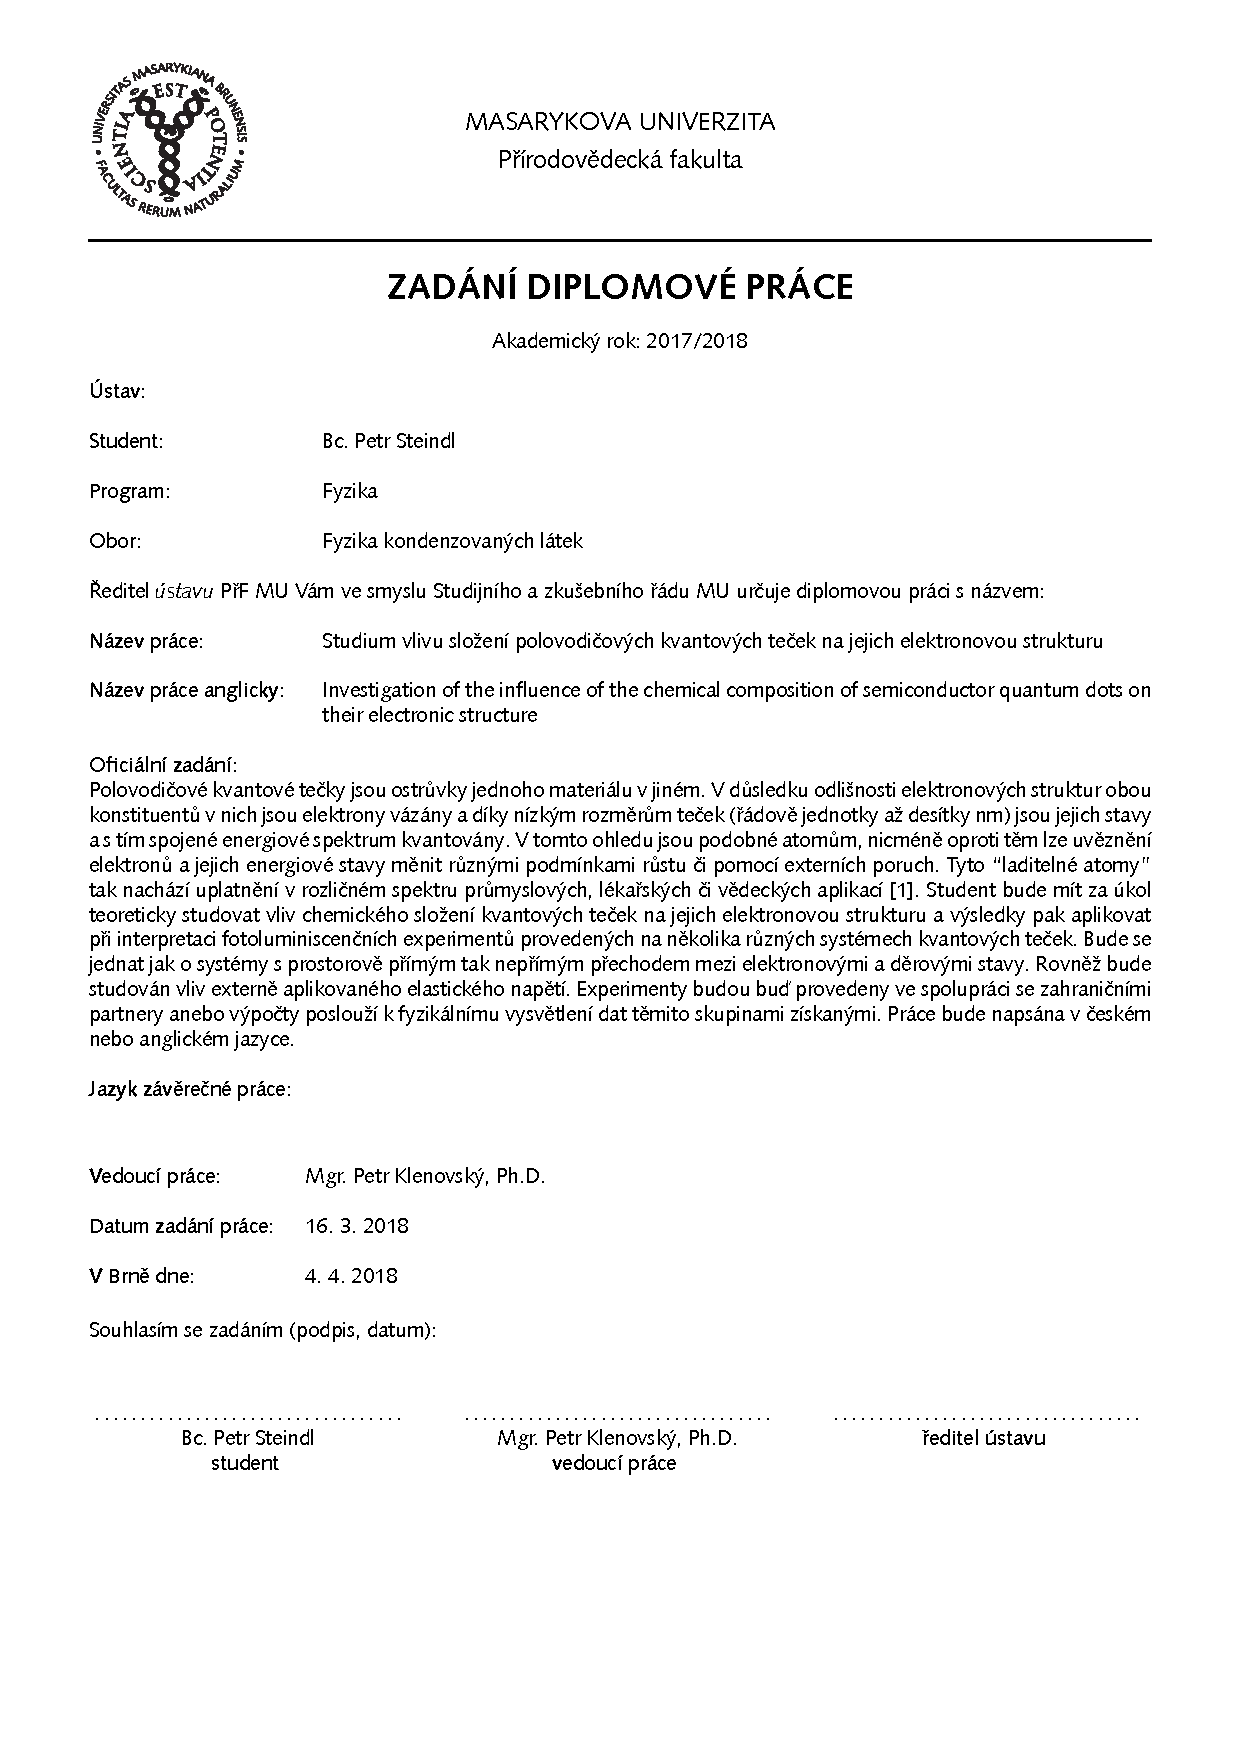
\includepdf[width=1.3\textwidth]{ofic_zadani_bezpodpisu.pdf}
\newpage

%\noindent\Large\textbf{Poděkování}\\ \normalsize

\noindent\Large\textbf{Acknowledgements}\\ \normalsize


\noindent I would like to express my sincere gratitude to my supervisor Dr. Petr Klenovský for the continuous support of my master study and related research, for his motivation, and guidance throughout this work. He also introduced me to the envelope function and configuration interaction methods. 

Besides my supervisor, many thanks belong to Prof. Thomas Fromherz for a kind welcome at Johannes Kepler University in Linz, for supporting me during my stay there and discussion around my theoretical results. I would like to thank also to Rinaldo's group, namely Johannes Aberl and Assoc. Prof. Rinaldo Trotta, from the same university for share their experimental results for theoretical description.

It is an honour for me to collaborate with Dr. Benito Millán Alen from Instituto de Micro~y~Nanotecnología of Spanish National Research Council. Under his leadership, I executed measurements on InGaAsSb/GaP quantum dots in his laboratory in Madrid.



This thesis would not have been possible unless there were samples, hence I am particularly grateful for their growing by Dr. Alice Hospodková from Institute of Physics of the Czech Academy of Science and by Dr. Elisa Maddalena Sala from Prof. Bimberg group in Technische Universität Berlin.

I thank Ing. Jan Michalička for assistance during TEM measurements at CEITEC Nano, all colleagues at Department of Condensed Matter Physics for mutual discussion of physics and Anna for language correction.


%\noindent I would like to express my sincere gratitude to my supervisor doc. Mgr. Norbert Werner, Ph.D. for his immense knowledge, encouragement, limitless patience, and guidance throughout this work. Besides my supervisor, many thanks belong to Mgr. Filip Hroch, Ph.D. for the priceless advice and support he has given me and to Kiran Lakhchaura for her valuable help with deprojection.\\
%\indent I am also very grateful for the possibility of participating in training lead by experts in X-ray astronomy and XMM-Newton issues in Netherlands Institute for Space Research SRON via funding of AHEAD Trans-National Access.

\vfill
\noindent\Large\textbf{Prohlášení}\\ \normalsize

\noindent Prohlašuji, že jsem svoji diplomovou práci vypracoval samostatně
s využitím informačních zdrojů, které jsou v práci citovány.
\vspace{1cm}
\begin{center}
	\centering
	\begin{tabular}{p{0.5\linewidth}p{0.15\linewidth}p{0.25\linewidth}}
		Brno 16.\,května\,2018 &  & \\\cmidrule[0.5pt]{3-3}
		&&\centering Podpis autora \\ 
	\end{tabular}
\end{center}

\newpage

%\begin{abstract}
%\lipsum[1-2]
%k tomuto textu je tu poznamka pod carou.\footnote{poznamka pod carou}
%\end{abstract}
%\clearpage


\pagestyle{standard}

\tableofcontents*


\clearpage




\chapter{Introduction}\label{chap:introduction}


Since 1980, when Russian physicist Ekimov first observed quantum dots on a glass crystal~\cite{Ekimov}, semiconductor research is expanding by studying quantum dots (QDs) which, due to the spatial limitation of electrons, exhibit properties depending on their shape and size. In 1984, the link between the size of the semiconductor nanoparticle and its forbidden band was derived by Luis Brus~\cite{Brus}, which triggered the QD decade ended with the successful synthesis of colloidal CDX (X = S, Se, Te) QD with a quantifiable absorbent edge~\cite{Murray}. Since the discovery, QDs have been mainly studied for a variety of optical applications. %In the 1990s, the QD study was mainly devoted to materials III-V, which are supposed to replace part of electrical circuits in the computer behind optical ones. %Historical details can be found eg in \cite{Bimberg}.

\section{Quantum confinement effect}
Semiconductor QDs are islands of semiconductor material of the size of nanometers or tens of nanometers in all three spatial directions embedded in the matrix of a different one. Because the size of these structures are comparable or smaller than the de Broglie wavelength of electron written as
\begin{equation}
\lambda=\frac{h}{\sqrt{(3m^*k_\mathrm{B}T)}},
\end{equation}
where $m^*$ is the effective mass, $h$ and $k_\mathrm{B}$ are the Planck and the Boltzmann constants, and $T$ is temperature, quantization effects begin to play an essential role of the QD properties. 


%
\begin{figure}
	\centering
	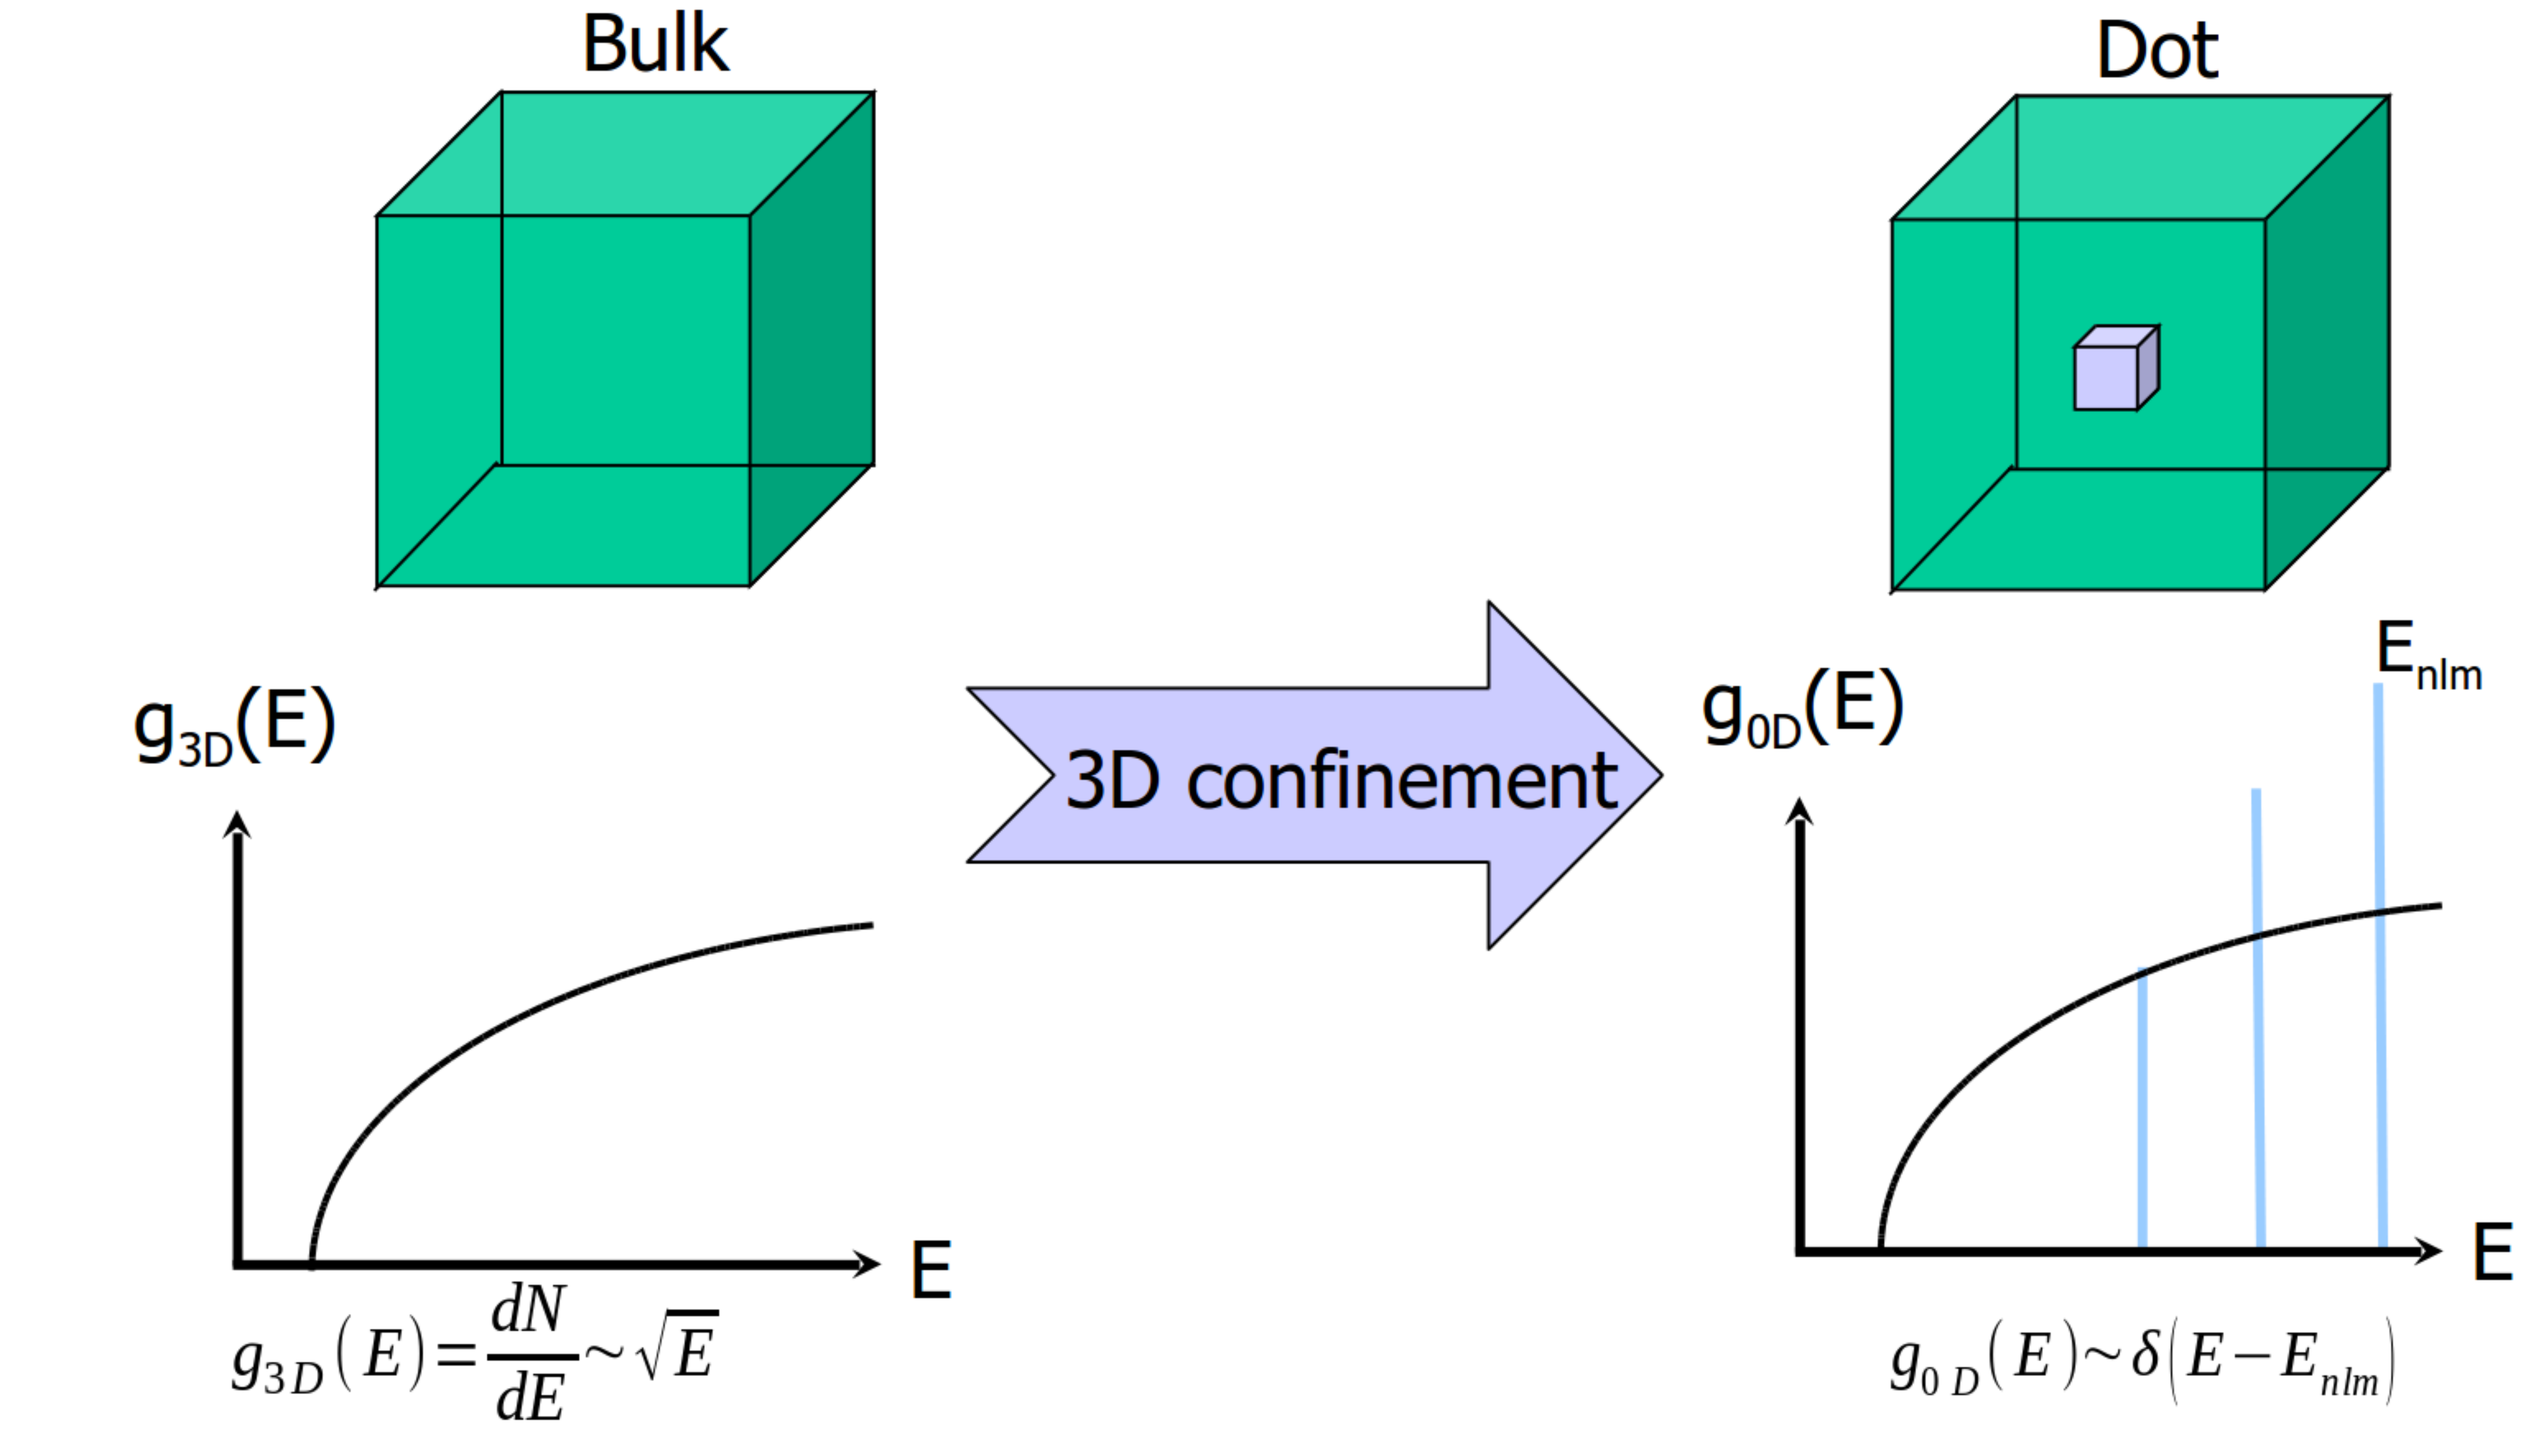
\includegraphics[width=0.8\linewidth]{/introduction/nizkodimense_dip2}
	\caption{Sketches of the bulk and QD structures (upper row) and the corresponding density of states (bottom row).}
	\label{fig:intr:nizkodimenze}
\end{figure}
%
While charge carriers in a bulk semiconductor are free to move in any spatial direction with density of states $g_{3D}$ proportional to $\sqrt{E}$ where $E$ is the energy of the carrier, QDs have the discrete energy spectrum due to 3D confinement and thus density of state of one QD $g_{0D}$ consists of a series of $\delta$-functions which is similar behaviour to that of individual atoms. However, unlike in atoms their energy spectrum can be tailored by the size, shape and composition of the QDs and of the surrounding material. Density of states of bulk and QD are shown in Fig.~\ref{fig:intr:nizkodimenze}.

\section{Preparation of QDs in heterostructures}
For a variety of applications are produced semiconductor heterostructures with contained QDs. These heterostructures formed by the alternation layers of different semiconductors can be fabricated with almost atomically-abrupt epitaxial layers due to the development of metalorganic vapour phase epitaxy (MOVPE)~\cite{Stringfellow,MOVPE_May} and molecular beam epitaxy (MBE)~\cite{Stringfellow,MOVPE_May}.

MOVPE uses organic precursors containing the chemical elements for the formation of the desired semiconductors. The precursors are injected in gaseous form into the reactor, where they deposit on the substrate which is kept at a high temperature to induce pyrolysis of the precursors. After pyrolysis, the required atoms form the epitaxial layer on the substrate whereas other products of pyrolytic reaction leave the reactor.



MBE technique yields crystals of higher purity and quality, but it is much slower than MOVPE. Constituents of the desired semiconductor are directly evaporated into an ultrahigh vacuum (UHV) chamber containing the substrate where are deposited an epitaxial layer from the molecular beams.

These techniques of epitaxial growth require in principle same lattice constant in the whole heterostructure. Because different semiconductor combined in the heterostructure present different lattice constant occurs during growth to compression or stretching of lattice constant of the material to match the one of the substrate which increase strain energy. % This strained growth produce a biaxial strain in the region near the interface which leads to a shift in the band edges~\cite{BirPik}. 
%If the thickness of epitaxial layer exceeds critical thickness, the energy stored into the strained bonds is relaxing into the material and creates dislocation which is undesirable in technological applications. 
%Relaxation does not usually occur in the whole epitaxial layer at once therefore accumulated strain can lead to a transition from two-dimensional to three-dimensional growth mode with the formation of islands where the strain is released.

 
If the epitaxial layer is thicker than the critical thickness, it is energetically favourable for structure to relax and increase the surface and thereby minimize its total energy, therefore, depending on the lattice mismatch % $f$ of materials defined by the unstrained lattice constants of substrate $a_0^\mathrm{sub}$ and the epitaxial layer $a_0^\mathrm{film}$ as
%\begin{equation}
%f=\frac{a_0^\mathrm{sub}-a_0^\mathrm{film}}{a_0^\mathrm{film}}
%\end{equation} 
can be differentiated three types of growth, see Fig.~\ref{fig:intr:growth}.
%
\begin{figure}
	\centering
	\includegraphics[width=0.8\linewidth]{/introduction/growth}
	\caption{Sketches of the three epitaxial growth modes: (a) Frank-von der Marwe, (b) Volmer-Weber, (c) Stranski-Krastanov. Taken from Ref.~\cite{t_bonato}.}
	\label{fig:intr:growth}
\end{figure}
%

For a structure with very little lattice mismatch is typical Frank-von der Marwe~\cite{Frank-Merwe}~[Fig.~\ref{fig:intr:growth}(a)] proceeds fully layer by layer atomically smooth growth with gradually relaxed strain and without formation of dislocations across the first few layers. On the other hand, the large mismatch causes that adatoms to prefer bonding with other adatoms before binding to the substrate resulting in the formation of non-contiguous islands in Volmer-Weber growth~\cite{Volmer-Weber}~[Fig.~\ref{fig:intr:growth}(b)]. Finally, Stranski-Krastanov growth~\cite{Stranski1937}~[Fig.~\ref{fig:intr:growth}(c)] represents mixture of the both previous modes. The adatoms first cover the substrate completely by wetting layer and then proceed to form three-dimensional islands of a size of nanometres, in other words, QDs. These QDs are self-organized, i.~e., without the need for further processing after growth is completed.


\section{Type-I vs type-II}
The band alignment of low-dimensional heterostructures is the key characteristic for designing electronic and optoelectronic devices. It was experimentally shown that there is no a priori relation between the band-edge energies of the semiconductors forming a heterojunction~\cite{Kroemer1985}. The problem is simplified if we need to clarify not the band offset values but only a type of confinement presented in the heterostructure, depending on used materials and interface structure, as: (i) type-I band alignment, where both electrons and holes are localized in the same layer and (ii) type-II, where are electrons and holes spatially separated and confined in neighbouring layers, see~Fig.~\ref{fig:intr:typeI_vs_typeII}.
%
\begin{figure}
	\centering
	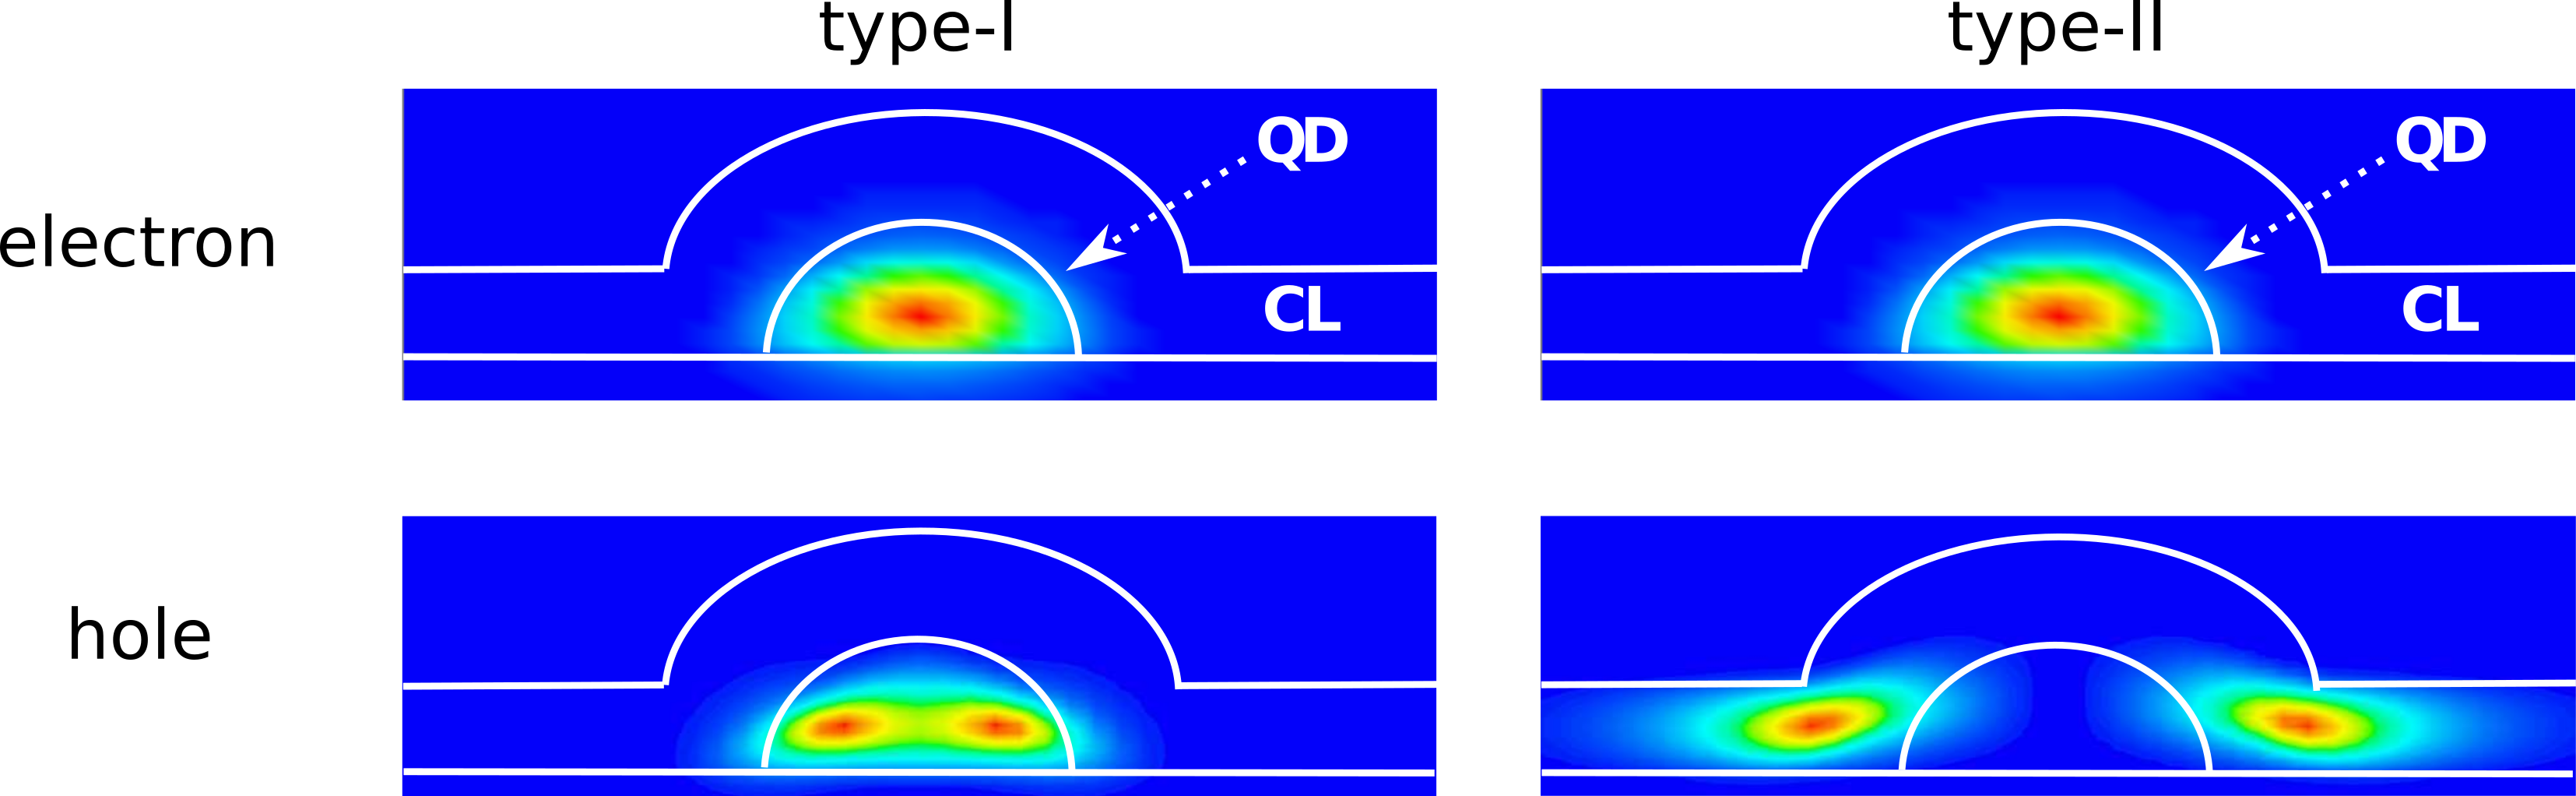
\includegraphics[width=0.8\linewidth]{/introduction/typeI-vs-typeII}
	\caption{Electrons and holes are depicted using probability density of their wavefunctions. The left column illustrates type-I confinement with both charge carriers localized in the body of QD and the right one shows case of type-II confinement with spatially separated charge carriers where electrons are confined in the QD body and holes in the CL.}
	\label{fig:intr:typeI_vs_typeII}
\end{figure}

For experimental ascertainment of the type of confinement in heterostructure can be used several experimental tools, such as X-ray photoemission spectroscopy~\cite{Lin2014}, internal photoemission~\cite{Zhang_2012}, or capacity-voltage technique~\cite{Brounkov_1996}. One of the most convenient methods is based on analysis of the emission energy shift $\Delta E$ of band with changing excitation density $P_\mathrm{ex}$ in photoluminescence spectra. %For both type of confinement can be observed blue-shift of emission energies but for type-II alignment is blue-shift more pronounced. \textit{Abrakin et al.} 


For heterostructures with type-II confinement, increasing the charge concentration with an increase in the excitation density leads to the distortion of the electrostatic potential of the charged layer, which is formed by spatially separated charge carriers (so-called the bend bending). The change of the electrostatic potential affects electron and hole quantum confinement energies and results in the blue-shift of the optical transition related to recombination of these charge carriers. The state filling, which occurs in both type-II and type-I band alignment, also leads to the blue-shift, thus the blue-shift can be observed in type-I. To distinguish these two effects in experimental data \textit{Abrakin et al.} have derived an analytical model~\cite{Abramkin_blueshift_analytical}
\begin{eqnarray}
\Delta E\left(P_\mathrm{ex}\right)=\left(U_e+U_h\right)\ln\left(P_\mathrm{ex}\right) + b\cdot P^{1/3},
\end{eqnarray}
where state filling effect is proportional to $\ln\left( P_\mathrm{ex} \right)$ and bend bending to $P_\mathrm{ex}^{1/3}$; $U_e$ ($U_h$) is the electron (hole) Urbach energy tail and $b$ is the bend bending parameter.




\section{Selected application}
The unique emission properties of QDs are used or planed to be used in a number of applications, some of which are chosen here and briefly presented.
\subsection*{Quantum dot laser}
Advantages of laser based on QD emitters in active region, compared to quantum well laser, are (i) very low threshold current, i.~e., the current needed to compensate for the power losses in the device; (ii) narrow spectral linewidth of their emission caused by the discrete density of states and (iii) high temperature stability. In general, there are two possibilities to create QDs laser.

In edge-emitting laser structures, QDs are sandwiched between two layers of material with a smaller refractive index, where the material with a lower index serves as a waveguide. During the growth are coating layer under and below QDs are doped for easy pumping electrically. In order to enhance the light output from the structure, multiple layers of QDs in active region are usually grown. Such lasers have been developed~\cite{Kirstaedter,SellinAPL,SellinEL,Kovsh,Ledentsov} and are currently used in the optical fiber communication, operating at communication wavelengths of 1.3 and 1.55~$\mathrm{\mu m}$~\cite{QDlaser}. 

The second possibility is surface-emitting QDs lasers, where active layer is thinner (smaller than 1~$\mu$m). This laser emits along the sample growth direction, i.~e., the cladding layers with smaller refractive index are not needed, however, there are bigger losses of light. An example of a device is described in detail in Ref.~\cite{Saito}.


\subsection*{Quantum dot memories}
QDs might be in the future efficiently used as substitution of nowadays broadly used computer memories, DRAM (Dynamic Random Access Memory) and Flash~\cite{Pavan,Sherwin}. DRAM has fast access time ($\sim$20~ns) and high endurance ($\sim10^{16}$ read/write cycles), but low storage time of tens of milliseconds, thus the data on the memory need to be permanently refreshed. Flash memory due to SiO$_2$ barrier around a metal oxide field effect transistor (MOSFET) gate, that serves as the storage unit in these memories, has high storage time, because the probability for electron of tunnel through SiO$_2$ barrier is small. However, it is also the reason for its low endurance ($\sim 10^{6}$ read/write cycles) because hot electrons need to be injected into it during writing of the data, slowly destroying the memory over time. 
%
\begin{figure}
	\centering
	\includegraphics[width=0.8\linewidth]{/introduction/QD-Flash}
	\caption{Summary of all storage times for holes at room temperature measured as of yet in self-organised QDs, plotted the respective localisation energies $E_\mathrm{loc}$. Each experimental point is marked with the material system. Parameter $\sigma$ is capture cross-section for self-organised QDs ($\sim10^{ -15} -10^ {-9}$~cm$^2$). The label \enquote{This work} indicate Bonato thesis from where the figure was taken from~Ref.~\cite{t_bonato}.}
	\label{fig:intr:QD-flash}
\end{figure}

QD-Flash is a concept of memory using a QD as a storage unit developed at Technische Universität Berlin by A.~Marent, M.P.~Geller and D. Bimberg~\cite{Marent_SST2011_QDFlash} which has been realized for several systems of QDs from III--V~materials, actual experimental results of storage time for holes are summarized in Fig.~\ref{fig:intr:QD-flash}~from Ref.~\cite{t_bonato}. The idea behind the memory cell is a QD surrounded by a barrier from other III--V~material with higher band gap and placed into a depletion layer of p-n or p-i-n diode. The write (erase) operation is realized by applying proper bias on the structure allowing tunnelling of electrons or holes into (out of) the structure. The reading is performed via a 2D~electron gas below the QDs. This type of memory is designed to have a read/write time comparable with DRAM memories (6~ns for InAs/GaAs QDs~\cite{GellerAPL}) and storage times similar to those of Flash memories (desired value is 10~years)~\cite{GellerAPL,GellerJOP}. Moreover, the carrier binding energies in QDs from III--V materials can be advantageously tuned. 

Because holes have a much larger effective mass than electrons~\cite{sze} leading to longer storage times for the same localisation energy $E_\mathrm{loc}$. For this reason, QD-Flash uses preferably type-II QDs which localise only holes, so that the entirety of the band gap mismatch can be exploited.

\subsection*{Quantum computing and cryptography}
Another application of QDs lies in the field of computers and cryptography~\cite{Feynman,Deutsch,Loss}. A number of implementations of quantum gates needed for quantum computing have been designed so far, see e.g.~\cite{Bennett}. For a realization of the qubit is frequently considered the spin of electrons for QDs~\cite{Loss} with which it is manipulated with optical methods~\cite{Hafenbrak} or magnetic field~\cite{Burkard}. 

In the present moment is a crucial step of realization of an entangled photon pair which was recently shown by tuning of the fine-structure splitting of an exciton emission from QD to zero by simultaneously applying external electric field and stress~\cite{Trotta}.

\vspace{0.2cm}
QDs are also used in other application such as the third generation of solar cells where QDs are added to increase absorption of light there leading to increase their efficiency up to 51.6~$\%$~\cite{Jiang_NonoEn2015_QDsolarcell}, to preparation of QD color filters for QD-liquid-crystal display (QD-LCD)~\cite{Chen_IEEE_2017_QLED}, or for biosensing and bioimaging~\cite{Li_JMaterChemB_2014_biosensing}.

\vspace{0.2cm}
In this work we study effects of the material composition of III--V semiconductor QDs on their electron structure. First of all in Chapter~\ref{chap:theory}, we demonstrate theoretical background of several approximations leading to the Envelope function theory usually used to simulate electronic structure of QDs and to the multiparticle states in the Configuration interaction method.

In Chapter~\ref{chap:2order_piezo} is investigated effect of second order piezoelectricity on electronic and excitonic structure of strain-tuned InGaAs/GaAs QDs by the eight-band $\mathbf{k \cdot p}$ and the Configuration interaction method.

Chapter~\ref{chap:SciRep} is focused to experimental study of excitonic structure of type-II InAs/GaAsSb/GaAs QDs by performing photoluminescence measurements and the blue-shift of emission energies of these structures is examined. Both excitonic structure and blue-shift is supported by multi-particle calculations.

Chapter~\ref{chap:TUB_QD} presents experimental study of electronic structure of InGaAsSb/GaAs/GaP QDs which is one of the promising candidate for long storage time and application in QD-Flash memories.   
\newpage 




\mainmatter

%%%%%%%%%%%%%%%%%%%%%%%%%%%%%%%%%%%%%%%%%%%%%%%%%%%%%%%%%%%%%%%%%%%%
%\input{introduction/introduction.tex}

\chapter{Theoretical calculations of electronic and excitonic structure of quantum dots}\label{chap:theory}

The Hamiltonian describing a perfect crystal can be written as 
\begin{eqnarray}
\mathcal{H}& =& \sum_{i}\frac{\mathbf{p}_i ^2}{2m_i} + \sum_{j}\frac{\mathbf{P}_j^2}{2M_j}+ \frac{1}{2}\sum_{j', j, j\neq j'}   \frac{Z_j Z_{j'}e^2}{4\pi \epsilon(\mathbf{R}_j, \mathbf{R}_{j'}) |\mathbf{R}_j-\mathbf{R}_{j'}|}  \nonumber \\
&+&\frac{1}{2}\sum_{i', i, i\neq i'} \frac{e^2}{4\pi \epsilon(\mathbf{r}_i, \mathbf{r}_{i'}) |\mathbf{r}_i-\mathbf{r}_{i'}|} - \sum_{j, i} \frac{Z_j e^2}{4\pi \epsilon(\mathbf{r}_i, \mathbf{R}_{j}) |\mathbf{r}_i-\mathbf{R}_{j}|}. \label{eq:HAM_idealni_krystal}
\end{eqnarray}
In the above expression the index $i$ ($j$) denotes summing over electrons (nuclei). The symbol $\mathbf{p}_i$ ($\mathbf{P}_j$) denotes momentum operator of the electrons (nuclei), $m_i$ ($M_j$) is the mass of electron (nucleus) $\mathbf{r}_i$ ($\mathbf{R}_j$) is the position of the $i$th electron ($j$th nucleus), $Z_j$ is the atomic number of the nucleus; $e$ and $\epsilon$ represent the elementary charge and the spatially dependent permittivity, respectively.

The many-particle Hamiltonian in (\ref{eq:HAM_idealni_krystal}) is currently unsolvable for realistic materials without approximations. In the following, we present necessary approximations usually made to describe quantum dots.

%%%%%%%%%%%%%%%%%%%%%%%%%%%%%%%%%%%%%%%%%%%%%%%%%%%%%%%%%
\section{Adiabatic approximation}
Ions are much heavier than electrons, thus, they move significantly more slowly. % than the electrons. 
Therefore, electrons can respond to nuclei movement almost immediately or, in other words, to the electrons ions seem as static background charges. On the other hand, nuclei cannot follow electrons' motion and they 'feel' only a time-averaged electronic potential. With the adiabatic approximation Hamiltonian Eq.~(\ref{eq:HAM_idealni_krystal}) can be simplified to

\begin{eqnarray}
\mathcal{H}=H_\mathrm{e}\left(\mathbf{r}_i,\mathbf{R}_{j0}\right)+H_{\mathrm{ions}}\left(\mathbf{R}_j\right)+H_{\mathrm{e-ion}}\left(\mathbf{r}_i,\delta\mathbf{R}_{j}\right),\label{eq:HAM_adiab}
\end{eqnarray}
%
where $H_\mathrm{e}\left(\mathbf{r}_i,\mathbf{R}_{j0}\right)$ is the Hamiltonian for electrons with frozen ions in their equilibrium positions $\mathbf{R}_{j0}$, $H_{\mathrm{ions}}\left(\mathbf{R}_j\right)$ represents ionic motion in potential of other ions plus average electronic potential. The third term in Eq.~(\ref{eq:HAM_adiab}) describes a change in the electronic energy as a result of displacement of ions by $\delta\mathbf{R}_{j}$ from their equilibrium position $\mathbf{R}_{j0}$. $H_{\mathrm{e-ion}}\left(\mathbf{r}_i,\delta\mathbf{R}_{j}\right)$ describes the so-called the electron-phonon interaction.

Therefore, in the adiabatic approximation we are looking for a solution of a wavefunction of the system of electrons and nuclei in the following form:
%
\begin{eqnarray}
\Psi\left(\mathbf{r}_i, \mathbf{R}_{j}\right)=\Psi_\mathrm{e}\left(\mathbf{r}_i,\mathbf{R}_{j0}\right)\Phi\left(\mathbf{R}_j\right),\label{eq:Psi_addiabatic}
\end{eqnarray}
%
where multi-particle wavefunction $\Psi\left(\mathbf{r}_i, \mathbf{R}_{j}\right)$ is a product of multi-particle electron wavefunction with ions in their lattice position $\Psi_\mathrm{e}\left(\mathbf{r}_i,\mathbf{R}_{j0}\right)$ and that of the static nuclei $\Phi\left(\mathbf{R}_j\right)$.

Equation~(\ref{eq:Psi_addiabatic}) allows us to solve the system of electrons described by $H_\mathrm{e}$ independently
\begin{equation}
H_\mathrm{e}\Psi_\mathrm{e}=E_\mathrm{e}\Psi_\mathrm{e},
\end{equation}
\begin{equation}
H_\mathrm{e}\left(\mathbf{r}_i,\mathbf{R}_{j0}\right)=\sum_{i} \frac{\mathbf{p}_i^2}{2m_i}- \sum_{j, i} \frac{Z_j e^2}{4\pi \epsilon(\mathbf{r}_i, \mathbf{R}_{j0}) |\mathbf{r}_i-\mathbf{R}_{j0}|} + \frac{1}{2}\sum_{i', i, i\neq i'} \frac{e^2}{4\pi \epsilon(\mathbf{r}_i, \mathbf{r}_{i'})  |\mathbf{r}_i-\mathbf{r}_{i'}|} .\label{eq: Ham_e}
\end{equation}
%
Because the ions are practically static, their effect on electrons can be described by a scalar potential $V_{\mathrm{e}-j0}\left(\mathbf{r}_i\right)$. With this simplification we can rewrite $H_\mathrm{e}$ in (\ref{eq: Ham_e}) as
\begin{equation}
H_\mathrm{e}=-\sum_{i} \frac{\hbar^2}{2m_i}\Delta_i+\sum_i V_{\mathrm{e}-j0}\left(\mathbf{r}_i\right) + \frac{1}{2}\sum_{i', i, i\neq i'} \frac{e^2}{4\pi \epsilon(\mathbf{r}_i, \mathbf{r}_{i'})  |\mathbf{r}_i-\mathbf{r}_{i'}|},\label{eq: Ham_e2}
\end{equation}
where we use the expression $\mathbf{p}_i=-\mathrm{i}\hbar\nabla_i$ and $\Delta_i$ is the Laplace operator operating on the $i$-th electron.



%%%%%%%%%%%%%%%%%%%%%%%%%%%%%%%%%%%%%%%%%%%%%%%%%%%%%%%%%
\section{Mean-field approximation}
Diagonalizing the hamiltonian $H_\mathrm{e}$ for $N$ electrons in the system (there are $>10^{23}$ electrons/cm$^3$ in a semiconductor) is currently an unsolvable task. To further simplify this problem we introduce the mean-field approximation, where we assume that each electron is influenced only by a mean electrostatic potential of the other electrons~$V\left(\mathbf{r}\right)$. Thus the Schrödinger equation describing the motion of each electron will be given by

\begin{eqnarray}
\left( -\frac{\hbar^2}{2m}\Delta +V\left( \mathbf{r}\right) \right) \psi_n\left(\mathbf{r}\right) = E_n \psi_n\left(\mathbf{r}\right), \label{eq:1el}
\end{eqnarray}
where $n$ labels eigenstates.


%%%%%%%%%%%%%%%%%%% 8-band kp
\section{8-band $\mathbf{k\cdot p}$ approximation}
\label{theor8kp}

The $\mathbf{k\cdot p}$ approximation was originally developed for calculations of the band structure of bulk semiconductors by Luttinger~\citep{Lutt} and Kane~\citep{Kane}. It is based on the fact that the most crucial properties of semiconductors come from the vicinity of the extrema of the valence and conduction band. Thus, the band structure can be reconstructed from the eigenstates at those extrema.

Now let us consider the solution of the Schrödinger equation (\ref{eq:1el}) for the crystalline solid with infinite periodic lattice. The potential acting on electrons is periodic with the periodicity of the lattice, i. e.

\begin{equation}
V(\mathbf{r}+\mathbf{R})=V(\mathbf{r}).
\end{equation}
The solution can then be searched for in accordance with the Bloch theorem as a product of plane wave and a function $u_{n\mathbf{k}}(\mathbf{r})$ with the periodicity of the crystalline lattice

\begin{eqnarray}
\psi_{n\mathbf{k}}\left( \mathbf{r} \right) = u_{n\mathbf{k}}\left(\mathbf{r}\right) \mathrm{e}^{\mathrm{i} \mathbf{k}\mathbf{r}}, \qquad u_{n\mathbf{k}}\left(\mathbf{r+R} \right) = u_{n\mathbf{k}}\left(\mathbf{r}\right).\label{eq:Bloch}
\end{eqnarray} 

If we insert (\ref{eq:Bloch}) into (\ref{eq:1el}) and act with the operator in round brackets on the Bloch function. We then arrive at the Schrödinger equation for the periodic part of wavefunction with the $\mathbf{k}\cdot\mathbf{p}$ term which gives name to the method

\begin{equation}
\left(-\frac{\hbar^2}{2m}\Delta+\frac{\hbar}{m}\mathbf{k}\cdot\mathbf{p}+\frac{\hbar^2 k^2}{2m}+V(\mathbf{r})\right)u_{n\mathbf{k}}(\mathbf{r})=E_nu_{n\mathbf{k}}(\mathbf{r}). \label{eq:kp}
\end{equation}

The solution of (\ref{eq:kp}) can be expanded as a superposition of all $u$-functions for any given $\mathbf{k}$ in the reciprocal space. For QDs fabricated from direct zinc-blende semiconductors, where the minimum of conductive and the maximum of valance band are situated at $\Gamma$ point of the Brillouin zone, usually $\mathbf{k}=0$ is selected and the expansion reads

\begin{equation}
\label{eqBlochSuper}
u_{n\mathbf{k}}(\mathbf{r})=\sum_i c_{ni}(\mathbf{k}) u_{i0}(\mathbf{r}).
\end{equation}

If we insert that into (\ref{eq:kp}), multiply both sides by $u_{j0}^*(\mathbf{r})$ and integrate over the unit cell, the equation reduces at $\Gamma$ point to 
\begin{equation}
\left(-\frac{\hbar}{2m}\Delta+V(\mathbf{r})\right)u_{n0}(\mathbf{r})=E_nu_{n0}(\mathbf{r}),
\end{equation}
and coefficients $c_{ni}$ are given by the equation

\begin{equation}
\sum_j\left[\left(E_i+\frac{\hbar k^2}{2m}\right) \delta_{ji}+\frac{\hbar}{m}\mathbf{k}\left<u_{j0}|\mathbf{p}|u_{i0}\right> +V(\mathbf{r}) \right]c_{nj}=E_nc_{ni}, \label{eq:koeficienty_schr}
\end{equation}
where also the orthogonality of the $u$-functions at $\Gamma$, i.e.~$\int u_{i0}(\mathbf{r})u_{j0}^*(\mathbf{r})\mathrm{d}\mathbf{r}=\delta_{ij}$ was used.

Using the full set of $u$-functions, the equation (\ref{eq:koeficienty_schr}) would provide an accurate description of the band structure in the whole Brillouin zone. However, in reality, the basis is contracted to a rather small size -- usually, the uppermost valance and the lowermost conduction bands at $\Gamma$ are chosen, other bands can be included as a perturbation. A very common choice to describe band structure is eight-band $\mathbf{k\cdot p}$ approximation. In this thesis, we use this approximation too.

For the eight-band $\mathbf{k\cdot p}$ approximation the $u$-functions are formed from antisymmetric combination of the $s$-type conduction band and three $p$-orbitals originating from three topmost valence bands. Motivated by Kane~\citep{Kane} we use the following ordering of the basis eigenfunctions with respect to spin (spin is represented by $\uparrow$ or $\downarrow$): $\{|s\uparrow\rangle, |x\uparrow\rangle, |y\uparrow\rangle, |z\uparrow\rangle, |s\downarrow\rangle, |x\downarrow\rangle, |y\downarrow\rangle, |z\downarrow\rangle\}$, where $p$-orbitals are indicated by their symmetry, i. e. $p_x$ we mark as $|x\rangle$. In this basis the hamiltonian is defined as 

\begin{equation}
H_{\mathrm{kp8}}=H_\mathrm{B}+H_\mathrm{D}+H_\mathrm{SO},\label{eq:ham8kp}%+H_{st},
\end{equation}
where $H_{\mathrm{B}}$ describes kinetic and potential energy connected with the basis Bloch states, $H_{\mathrm{D}}$ describes the same for the distant bands which are added as a perturbation and $H_{\mathrm{SO}}$ introduces the spin-orbit coupling. The individual Hamiltonians, taken from Ref.~\citep{t_stier}, only as upper triangular Hermitian matrices are written in the following expressions.

\begin{equation}
H_\mathrm{B}=
\begin{pmatrix}
E_\mathrm{c}& \mathrm{i}Pk_x& \mathrm{i}Pk_y& \mathrm{i}Pk_z& 0& 0& 0& 0\\
& E_\mathrm{v}& 0& 0& 0& 0& 0& 0\\
& & E_\mathrm{v}& 0& 0& 0& 0& 0\\
& & & E_\mathrm{v}& 0& 0& 0& 0\\
& & & & E_\mathrm{c}& \mathrm{i}Pk_x& \mathrm{i}Pk_y& \mathrm{i}Pk_z\\
& & & & & E_\mathrm{v}& 0& 0\\
& & & & & & E_\mathrm{v}& 0\\
& & & & & & & E_\mathrm{v}\\
\end{pmatrix},
\end{equation}
where $E_\mathrm{c}$ and $E_\mathrm{v}$ represent conduction and valence band energies at $\Gamma$ point, respectively, and $P$ symbolizes the optical matrix element, $P=\langle s|p_x|x\rangle=\langle s|p_y|y\rangle=\langle s|p_z|z\rangle$.

The distant bands are described by
%
\begin{equation}
H_\mathrm{D}=
\begin{pmatrix}
A'\mathbf{k}^2& Bk_yk_z& Bk_xk_z& Bk_xk_y& 0& 0& 0& 0\\
& K_x& N'k_xk_y& N'k_xk_z& 0& 0& 0& 0\\
& & K_y& N'k_yk_z& 0& 0& 0& 0\\
& & & K_z& 0& 0& 0& 0\\
& & & & A'\mathbf{k}^2& Bk_yk_z& Bk_xk_z& Bk_xk_y\\
& & & & & K_x& N'k_xk_y& N'k_xk_z\\
& & & & & & K_y& N'k_yk_z\\
& & & & & & & K_z\\
\end{pmatrix},
\end{equation}
where e.~g., $K_x$ is defined by equation
\begin{eqnarray*}
	K_x=L'k_x^2+M(k_y^2+k_z^2),\nonumber\\
\end{eqnarray*}
the equations for $K_y$ and $K_z$ are identical except for cyclic index permutation; $A'$ and $B$ are the Kane parameters~\citep{Kane} and $N'$, $L'$, $M$ are the Dresselhaus parameters~\citep{Dress}.

The spin-orbit Hamiltonian has form
\begin{equation}
H_\mathrm{SO}=
\begin{pmatrix}
0& 0& 0& 0& 0& 0& 0& 0\\
& 0& -\mathrm{i}\frac{\Delta_0}{3}& 0& 0& 0& 0& \frac{\Delta_0}{3}\\
& & 0& 0& 0& 0& 0& -\mathrm{i}\frac{\Delta_0}{3}\\
& & & 0& 0& -\frac{\Delta_0}{3}& \mathrm{i}\frac{\Delta_0}{3}& 0\\
& & & & 0& 0& 0& 0\\
& & & & & 0& -\mathrm{i}\frac{\Delta_0}{3}& 0\\
& & & & & & 0& 0\\
& & & & & & & 0\\
\end{pmatrix},
\end{equation}
where $\Delta_0$ is the spin-orbit split-off energy. The other parameters present in the Hamiltonian $H_{kp8}$ are assigned to the material parameters used as input values in our calculations by the following equations

\begin{eqnarray}
E_c&=&E_0+E_v,\nonumber\\
P&=&\sqrt{\frac{\hbar^2}{2m}E_p},\nonumber\\
A'=\frac{\hbar^2}{2m}S&=&\frac{\hbar^2}{2m}\left(\frac{1}{m}-E_p\frac{E_0+\frac{2}{3}\Delta_0}{E_0(E_0+\Delta_0)}\right).\nonumber\\
\end{eqnarray}
{\noindent The summary of all input parameters is listed in Tab.~\ref{tDesc} in Sec.~\ref{Secsumparam}.}
 

%%%%%%%%%%%%%%%%%%%%%%%%%%%%%%%%%%%%%%%%%%%%%%%%%%%%%%%%%


\section{Envelope function theory}
\label{secTheorEnvelope}
% do sem to kontrolovala Anicka

In the previous part, we described the calculation of infinitely large and absolutely periodic crystal. However, the real heterostructures have neither of these properties. Their dimensions typically vary from a few to hundreds of nanometres and they are composed of several various materials, which breaks the assumption of periodicity, so the Bloch theorem cannot be used for these systems. To describe these structures we rather use the envelope function approximation.

The method was originally developed to describe the effect of a weak smooth external field $V_{\rm ext}$ acting on the bulk semiconductor, where $V_{\rm ext}$ can be viewed as a departure from periodicity, or a perturbation of the infinitely large and absolutely periodic crystal described by  $H_\mathrm{8kp}$ in (\ref{eq:ham8kp}). We search for the solution of the following Schr\"{o}dinger equation

\begin{equation}
(H_\mathrm{8kp}+V_{\rm ext})\Psi(\mathbf{r})=E\Psi(\mathbf{r}), \label{eq:H_envelope}
\end{equation}
where $\Psi(\mathbf{r})$ is chosen in the basis set composed from Bloch functions $\psi_{n0}(\mathbf{r})$ at the $\Gamma$ point. The solution of Eq.~(\ref{eq:H_envelope}) can be then expanded in the form
 
 \begin{equation}
 \label{eqEnvelope}
 \Psi(\mathbf{r})=\sum_{n=1}^8 F_n(\mathbf{r})\psi_{n0}(\mathbf{r}),
 \end{equation}
where Bloch functions are modulated by slowly varying (in comparison to the Bloch function) coefficients $F_n(\mathbf{r})$ called the envelope functions. After expansion of the external potential $V_\mathrm{ext}$ and the envelope functions $F_n(\mathbf{r})$ into terms of Fourier series and transformation of the Hamiltonian into the real space we arrive at a formally similar Hamiltonian as (\ref{eq:ham8kp}), except for $\mathbf{k}$-vector replaced by $-\mathrm{i}\nabla$. For derivation we refer to Refs.~\citep{Bastard1,Bastard2}. If we introduce the substitution $\mathbf{k}\rightarrow -\mathrm{i}\nabla$, the resulting Hamiltonian is not Hermitian because of spatially dependent material parameters. Eppenga~\citep{Eppenga} suggested the following symmetrization to overcome this problem
\begin{eqnarray}
Qk_i&\rightarrow&-\mathrm{i}\left(\frac{Q\partial_i+Q\partial_j}{2}\right),\nonumber\\
Qk_ik_j&\rightarrow&-\mathrm{i}\left(\frac{\partial_iQ\partial_j+\partial_jQ\partial_i}{2}\right),\nonumber\\
i,j&=&x,y,z,\nonumber
\end{eqnarray}
where $Q$ substitutes the spatially dependent material parameters. 

For completeness, we add the following note. The effective potential for electrons and holes in the heterostructures is formed by the band offsets and it is rather step-like at the interfaces of different materials than smooth as presumed by the above-described envelope function theory. There have been efforts to solve this problem by a number of authors (e.g.~Ref.~\citep{MlinarEnvelope}) though we rely on the extended use of the presented conventional envelope function approach and adopt it in this work. 
%%%%%%%%%%%%%%%%%%%%%%%%%%%%%%%%%%%%%%%%%%%%%%%%%%%%%%%%%

\subsection{Inclusion of the elastic strain}

The quantum dots prepared by self-organization are essentially strained due to the lattice mismatch between the constituents of the heterostructure. The strain shifts energies of the bands in QDs, mixes heavy and light hole states and contributes to the anisotropy of electron and hole wavefunctions. On the other hand, the wavefunctions and their energies can be tuned by externally applied strain. Thus induced elastic strains must be introduced to the calculations, e.~g., by adding the Pikus-Bir Hamiltonian~\citep{BirPik} to the envelope function Hamiltonian. The strain Hamiltonian $H_\mathrm{st}$ then reads
%Another effect on the electron structure in heterostructures is caused by lattice mismatch between the constituent materials. Thus induced elastic strain, especially for QDs, has a notable role in this structures. Strain effect enters the calculations via adding the Pikus-Bir Hamiltonian~\citep{BirPik} to the envelope function Hamiltonian. The strain Hamiltonian $H_\mathrm{st}$ reads

\begin{equation}
H_\mathrm{st}=
\begin{pmatrix}
D_s& ND_{sx}& ND_{sy}& ND_{sz}& 0& 0& 0& 0\\
& D_x& n\eta_{xy}& n\eta_{xz}& 0& 0& 0& 0\\
& & D_y& n\eta_{yz}& 0& 0& 0& 0\\
& & & D_z& 0& 0& 0& 0\\
& & & & D_s& ND_{sx}& ND_{sy}& ND_{sz}\\
& & & & & D_x& n\eta_{xy}& n\eta_{xz}\\
& & & & & & D_y& n\eta_{yz}\\
& & & & & & & D_z\\\end{pmatrix}.
\end{equation}
The symbols $\eta_{ij}$ ($i,j=x,y,z$) are the elements of elastic strain tensor and the other parameters are

\begin{eqnarray*}
	D_s=a_c(\eta_{xx}+\eta_{yy}+\eta_{zz}),\nonumber\\
	D_i=l\eta_{ii}+m(\eta_{jj}+\eta_{kk}),\nonumber\\
	ND_{si}=b'\eta_{jk}-\mathrm{i}P\sum_\alpha\eta_{i\alpha}k_\alpha,\nonumber\\
\end{eqnarray*}
where $i,j,k=x,y,z$; $a_c$ and $b'$ are the absolute and uniaxial shear deformation potentials of the conduction band, respectively. The absolute deformation potential for valence band $a_v$ and the shear deformation potential of valence band in the $[100]$ and $[111]$ crystallographic direction are expressed in the following relations

\begin{eqnarray*}
	&l=2a_{ub}+a_v,\nonumber\\
	&m=a_v-a_{ub},\nonumber\\
	&n=\sqrt{3}a_{ud}.\nonumber\\
\end{eqnarray*}





%%%%%%%%%%%%%%%%%%%%%%%%%%%%%%%%%%%%%%%%%%%%%%%%%%%%%%%%%
\subsection{Inclusion of the piezoelectricity}
\label{subPiezo}

%Piezoelectricity is an ability of a material without the inversion symmetry, which is specific in zinc-blende {III-V}~semiconductors~\citep{Hubner,Zeller,Gironcoli,KingSmith} like InAs, GaAs and GaSb, to generate electric charge if it is under mechanical stress.


Piezoelectricity is an ability of a material to generate an electric charge under mechanical stress. In zinc-blende {III-V}~semiconductors~\citep{Hubner,Zeller,Gironcoli,KingSmith} like InAs, GaAs and GaSb, it is induced by both spontaneous polarization caused by breaking the inversion crystal symmetry and piezoelectric polarization resulting from mutual displacement of the positively and negatively charged atoms. Therefore, including the piezoelectric effect improves the results of the $\mathbf{k}\cdot\mathbf{p}$ calculations.

The electric polarization $\mathbf{P}_{{\rm piezo}}$ can be expanded in the Taylor series of a strain tensor $\eta$ as
\begin{equation}
\mathbf{P}_{{\rm piezo},\mu}(\mathbf{r})=%\sum_{j} e_{\eta j}(\mathbf{r})\epsilon_{j}(\mathbf{r}),
\sum_je_{\mu j}\eta_j+\frac{1}{2}\sum_{jk}B_{\mu jk}\eta_j\eta_k+\dots ,\label{eq:second_order}
\end{equation}
where $e_{\mu j}$ represents linear and $B_{\mu jk}$ quadratic piezoelectric coefficients, $\eta$-s are indexed according to the Voigt notation (i.e. $\eta_1=\eta_{xx}$, $\eta_2=\eta_{yy}$, $\eta_3=\eta_{zz}$, $\eta_4=2\eta_{yz}$, $\eta_5=2\eta_{xz}$, $\eta_6=2\eta_{xy}$)~\citep{voigt_notation, Beya-Wakata2011}. 
Usually, for description of the effect of piezoelectricity only the first term in the previous expansion (\ref{eq:second_order}) is chosen, where the linear piezoelectric coefficient $e_{\mu j}$ for zinc-blende materials is reduced to one component $e_{14}$ and we, thus, have
\begin{equation}
\mathbf{P}_{{\rm piezo},1}(\mathbf{r})=%\sum_{j} e_{\eta j}(\mathbf{r})\epsilon_{j}(\mathbf{r}),
e_{14 }\eta_4 \label{eq:first_order}.
\end{equation}
%
Thereafter, according to the Coulomb law, the piezoelectric charge $\rho_{\rm piezo}(\bf{r})$ can be written using the divergence of displacement field $\bf{ D}$ in case if the external electric field is not affected ($\mathbf{D}=\mathbf{P}_\mathrm{piezo}$) leading to the Poisson equation

\begin{eqnarray}
\rho_{\rm piezo}(\mathbf{r})&=&\nabla\times\mathbf{P}_{\rm piezo}(\mathbf{r})=\epsilon_0\nabla\left[\epsilon_r(\mathbf{r})\nabla V_{\rm piezo}(\mathbf{r})\right],\\
\Delta V_{\rm piezo}(\mathbf{r})&=&\frac{\rho_{\rm piezo}(\mathbf{r})}{\epsilon_0\epsilon_r(\mathbf{r})}-\frac{1}{\epsilon_r(\mathbf{r})}\nabla V_{\rm piezo}(\mathbf{r})\cdot\nabla\epsilon_r(\mathbf{r}),
\end{eqnarray}
%
where $\epsilon_r(\bf{r})$ is the spatially dependent static dielectric function and $V_{\rm piezo}(\bf{r})$ is the piezoelectric potential. The most considerable effect of the piezoelectric potential to one-particle eigenstates is their elongation in $[110]$ or $[1\overline{1}0]$ directions~\citep{Stier1999} which has consequences such as the fine structure splitting (FSS) of the bright excitonic states. FSS is an undesirable phenomenon preventing a creation of entangled photon pairs from single QDs required to realize, e.~g., a single photon source. To reduce FSS, several experimental methods have been tried including InAs QDs growth on $[111]$~substrates~\citep{StockFSS}, fabrication of strain-free GaAs/AlGaAs~\citep{Abbarchi_2008} QDs with zero piezoelectric field or tuning FSS to zero by external fields: electric~\citep{Gerardot_2007, Vogel_2007}, magnetic~\citep{Stevenson_2006} or strain~\citep{kleDresden}. 

There are several works devoted to the influence of the quadratic or higher contributions of the dependence of $\mathbf{P}_{{\rm piezo}}$ on the strain tensor. They have found that these terms might be dominating compared to the first order-ones in III-V~semiconductors~\citep{Bester,Bester:06,Beya-Wakata2011}. We will study the effect of the second order piezoelectricity on electric dipole in strain-tuned InGaAs/GaAs QDs in section~\ref{sec:2order_piezo}.



%%%%%%%%%%%%%%%%%%%%%%%%%%%%%%%%%%%%%%%%%%%%%%%%%%%%%%%%%




%%%%%%%%%%%%%%%%%%%%%%%%%%%%%%%%%%%%%%%%%%%%%%%%%%%%%%%%%







\section{Summary of all input parameters for single-particle calculations}
\label{Secsumparam}

All material parameters entering the calculations of the single-particle states in this thesis are listed in the following table.

\begin{table}[!ht]
	\begin{tabular}{lc}
		\hline \hline
		Parameter & Description\\
		\hline
		$a$& lattice constant\\
		$a_{\rm exp}$& lattice thermal expansion coefficient\\
		$C_{11}$& elastic constant\\
		$C_{12}$& elastic constant\\
		$C_{44}$& elastic constant\\
		$e_{14}$& linear piezoelectric constant\\
		$B_{114}$& quadratic piezoelectric constant\\
		$B_{124}$& quadratic piezoelectric constant\\
		$B_{156}$& quadratic piezoelectric constant\\
		$\varepsilon_{r}$& static dielectric constant\\
		$E_0$& bandgap\\
		$\alpha$& Varshni parameter~\citep{Varshni}\\
		$\beta$& Varshni parameter~\citep{Varshni}\\
		$E_v$& valence band offset\\
		$\Delta_0$& spin-orbit split-off energy\\
		$a_c$& absolute deformation potential for conduction band\\
		$a_v$& absolute deformation potential for valence band\\
		$b'$& uniaxial shear deformation potential of the conduction band\\
		$a_{ub}$& uniaxial shear deformation potential of the valence bands  in the $[100]$ direction\\
		$a_{ud}$& uniaxial shear deformation potential of the valence bands in the $[111]$ direction\\
		$S$& electron effective mass parameter\\
		$E_p$& Kane's momentum matrix element\\
		$L$& Dresselhaus parameter~\citep{Dress}; $L=-\gamma_1-4\gamma_2-1$\\
		$L'$& reduced Dresselhaus parameter~\citep{Dress}; $L'=- \gamma_1 - 4\gamma_2 - 1 + \frac{E_p}{E_0+\frac{\Delta_0}{3}}$\\
		$M$& Dresselhaus parameter~\citep{Dress}; $M=2\gamma_2 - \gamma_1  - 1$\\
		$N$& Dresselhaus parameter~\citep{Dress}; $N=-6\gamma_3$\\
		$N'$& reduced Dresselhaus parameter~\citep{Dress}; $N'=-6\gamma_3 + \frac{E_p}{E_0+\frac{\Delta_0}{3}}$\\
		\hline \hline
	\end{tabular}
	\caption{Description of the material parameters used in the calculations; $\gamma_1$, $\gamma_2$ and $\gamma_3$ are the Luttinger parameters~\citep{Lutt}. Note that all parameters are spatially dependent. The table is taken from the thesis~\citep{t_klenovsky}. \label{tDesc}}
\end{table}


%%%%%%%%%%%%%%%%%%%%%%%%%%%%%%%%%%%%%%%%%%%%%%%%%%%%%%%%%
\section{Multiparticle states}
%
Until this point, we have restricted ourselves only to a single particle description. However, excited QDs are commonly occupied not by single but several charge carriers that interact with each other and form so-called multiparticle states. The most notable of these multiparticle excitations are excitons (bound electron-hole pair), charged excitons (trions) and biexcitons which significantly influence QD emission properties and understanding of them is essential. To produce these multiparticle complexes single-particle basis states might be used, like those obtained by the eight-band~$\bf{k\cdot p}$ method. The way to create the multiparticle states from this basis depends on the method used. In the following we outline a few of them.

\subsection{Hartree method}
The simplest approximation for setting-up of the multiparticle wavefunctions is based on the expansion into a direct product of the single-particle states and the multiparticle wavefunction $\Psi_\mathrm{H}$ in this so-called Hartree approximation~\citep{Ashcroft, Hartree_1928} with single-particle electron $\psi_{\rm{e}}$ and hole $\psi_{\rm{h}}$ wavefunctions is 


\begin{equation}
\label{hartree}
\Psi_\mathrm{H}=\psi_{\rm{e}}(\mathbf{r}_{\rm{e}})\psi_{\rm{h}}(\mathbf{r}_{\rm{h}}).
\end{equation}
%
Solution of the stationary Schrödinger equation with $\Psi_\mathrm{H}$ describes the excitonic structure respecting the direct Coulomb interaction between the charged particles. This approximation fails to describe the exchange interaction and correlation, and violates Pauli exclusion principle. The reasons were firstly pointed out by Slater and Fock: $\Psi_\mathrm{H}$ is not antisymmetric, hence it cannot describe the exchange.


\subsection{Hartree-Fock method}
To overcome the lack of antisymmetry in Hartree method the Hartree wavefunction was improved by Fock into Hartree-Fock approximation where the multi-particle function is constructed as a so-called Slater determinant (SD). The electron-hole pair in this approach reads 
%
\begin{equation}
\Psi_\mathrm{HF}=\frac{1}{\sqrt{2}}\begin{vmatrix}
\psi_{\rm{e}}(\mathbf{r}_{\rm{e}})&\psi_{\rm{h}}(\mathbf{r}_{\rm{e}})\\
\psi_{\rm{e}}(\mathbf{r}_{\rm{h}})&\psi_{\rm{h}}(\mathbf{r}_{\rm{h}})\\
\end{vmatrix}=\frac{1}{\sqrt{2}}\Big[\psi_{\rm{e}}(\mathbf{r}_{\rm{e}})\psi_{\rm{h}}(\mathbf{r}_{\rm{h}})-\psi_{\rm{e}}(\mathbf{r}_{\rm{h}})\psi_{\rm{h}}(\mathbf{r}_{\rm{e}})\Big].
\end{equation}
%
By applying this approximation, we correctly describe not only the direct Coulomb interaction caused by the influence of one charge carrier on the effective Coulomb potential from the remaining particle but also via so-called exchange term $\psi_{\rm{e}}(\mathbf{r}_{\rm{h}}) \psi_{\rm{h}}(\mathbf{r}_{\rm{e}})$. This approach still does not describe the correlation effects originated from the interaction of two equally charged particles with the same spin. To include those effects, the multi-particle wavefunction can be expanded into the series of the Slater determinants which is a fundamental principle of the configuration interaction (CI) method~\citep{t_stier}.

\subsection{Configuration interaction method}\label{Sec:CI}
In this method multiparticle wavefunction is expanded into SD base and consequently the stationary Schrödinger equation is solved in the form
\begin{equation}
\label{eq:CISchroedinger}
\hat{H}^M\left|M\right>=E^M\left|M\right>,\,\,M\equiv X^0, X^+, X^-, XX^0\dots,
\end{equation}
%
where $E^M$ is the eigenenergy of the (multi-)excitonic state $\left|M\right>$ describing the multi-particle complex with $N_{\rm{e}}$ electrons and $N_{\rm{h}}$ holes. In the following, examples of the wave functions for selected complexes, that are explored in this thesis, are listed. For the neutral exciton $X^0$ ($N_{\rm{e}}=1$, $N_{\rm{h}}=1$), we have
%
\begin{equation}
\label{eq:suppl:CIWavefunctionX}
\left|X^0\right>=\sum^{n_{\rm{e}}}_{i=1}\sum^{n_{\rm{h}}}_{j=1}\zeta_{ij}
\begin{vmatrix}
\psi_{{\rm{e}}i}(\mathbf{r}_{\rm{e}})&\psi_{{\rm{h}}i}(\mathbf{r}_{\rm{e}})\\
\psi_{{\rm{e}}j}(\mathbf{r}_{\rm{h}})&\psi_{{\rm{h}}j}(\mathbf{r}_{\rm{h}})\\
\end{vmatrix},
\end{equation}
%
for the positive trion $X^+$ ($N_{\rm{e}}=1$, $N_{\rm{h}}=2$)
%
\begin{equation}
\label{eq:suppl:CIWavefunctionX+}
\left|X^+\right>=
\sum^{n_{\rm{e}}}_{i=1}\,\sum^{n_{\rm{h}}}_{\substack{j,k=1\\k>j}}\zeta^+_{ijk}
\begin{vmatrix}
\psi_{{\rm{e}}i}(\mathbf{r}_{\rm{e}})&\psi_{{\rm{h}}j}(\mathbf{r}_{{\rm{e}}})&\psi_{{\rm{h}}k}(\mathbf{r}_{{\rm{e}}})\\
\psi_{{\rm{e}}i}(\mathbf{r}_{{\rm{h}}1})&\psi_{{\rm{h}}j}(\mathbf{r}_{{\rm{h}}1})&\psi_{{\rm{h}}k}(\mathbf{r}_{{\rm{h}}1})\\
\psi_{{\rm{e}}i}(\mathbf{r}_{{\rm{h}}2})&\psi_{{\rm{h}}j}(\mathbf{r}_{{\rm{h}}2})&\psi_{{\rm{h}}k}(\mathbf{r}_{{\rm{h}}2})\\
\end{vmatrix},
\end{equation}
%
for the negative trion $X^-$ ($N_{\rm{e}}=2$, $N_{\rm{h}}=1$)
%
\begin{equation}
\label{eq:suppl:CIWavefunctionX-}
\left|X^-\right>=
\sum^{n_{\rm{e}}}_{\substack{i,j=1\\j>i}}\,\sum^{n_{\rm{h}}}_{k=1}\zeta^-_{ijk}
\begin{vmatrix}
\psi_{{\rm{e}}i}(\mathbf{r}_{{\rm{e}}1})&\psi_{{\rm{e}}j}(\mathbf{r}_{{\rm{e}}1})&\psi_{{\rm{h}}k}(\mathbf{r}_{{\rm{e}}1})\\
\psi_{{\rm{e}}i}(\mathbf{r}_{{\rm{e}}2})&\psi_{{\rm{e}}j}(\mathbf{r}_{{\rm{e}}2})&\psi_{{\rm{h}}k}(\mathbf{r}_{{\rm{e}}2})\\
\psi_{{\rm{e}}i}(\mathbf{r}_{{\rm{h}}})&\psi_{{\rm{e}}j}(\mathbf{r}_{{\rm{h}}})&\psi_{{\rm{h}}k}(\mathbf{r}_{{\rm{h}}})\\
\end{vmatrix},
\end{equation}
%
and for the neutral biexciton $XX^0$ ($N_{\rm{e}}=2$, $N_{\rm{h}}=2$)
%
\begin{equation}
\label{eq:suppl:CIWavefunctionXX}
\left|XX^0\right>=
\sum^{n_{\rm{e}}}_{\substack{i,j=1\\j>i}}\,\sum^{n_{\rm{h}}}_{\substack{k,l=1\\k>l}}\zeta^{XX}_{ijkl}
\begin{vmatrix}
\psi_{{\rm{e}}i}(\mathbf{r}_{{\rm{e}}1})&\psi_{{\rm{e}}j}(\mathbf{r}_{{\rm{e}}1})&\psi_{{\rm{h}}k}(\mathbf{r}_{{\rm{e}}1})&\psi_{{\rm{h}}l}(\mathbf{r}_{{\rm{e}}1})\\
\psi_{{\rm{e}}i}(\mathbf{r}_{{\rm{e}}2})&\psi_{{\rm{e}}j}(\mathbf{r}_{{\rm{e}}2})&\psi_{{\rm{h}}k}(\mathbf{r}_{{\rm{e}}2})&\psi_{{\rm{h}}l}(\mathbf{r}_{{\rm{e}}2})\\
\psi_{{\rm{e}}i}(\mathbf{r}_{{\rm{h}}1})&\psi_{{\rm{e}}j}(\mathbf{r}_{{\rm{h}}1})&\psi_{{\rm{h}}k}(\mathbf{r}_{{\rm{h}}1})&\psi_{{\rm{h}}l}(\mathbf{r}_{{\rm{h}}1})\\
\psi_{{\rm{e}}i}(\mathbf{r}_{{\rm{h}}2})&\psi_{{\rm{e}}j}(\mathbf{r}_{{\rm{h}}2})&\psi_{{\rm{h}}k}(\mathbf{r}_{{\rm{h}}2})&\psi_{{\rm{h}}l}(\mathbf{r}_{{\rm{h}}2})\\
\end{vmatrix},
\end{equation}
%
where $\psi(\mathbf{r}_{{\rm{e}}})$ and $\psi(\mathbf{r}_{{\rm{h}}})$ are single-particle wavefunctions for electron and hole, respectively. Note that the set of (multi-)excitonic wavefunctions defined in Eqs.~(\ref{eq:suppl:CIWavefunctionX}-\ref{eq:suppl:CIWavefunctionXX}) is not normalized.

The Hamiltonian $H^M$ in Schrödinger equation~(\ref{eq:CISchroedinger}) may be written as sum of non-interacting Hamiltonian $\hat{H}_0^M$ and interacting term $\hat{V}^M$
%
\begin{equation}
\hat{H} ^M= \hat{H}_0^M + \hat{V}^M = \hat{H} _0^M + \sum_{\substack{s, t \in \{1 \ldots N_{{\rm{e}}}+N_{{\rm{h}}} \}\\t>s} } \hat{V}(\mathbf{r}_s,\mathbf{r}_t), 
\end{equation}
%
where interacting part of $H^M$ is composed of the contributions of the mutual Coulomb interaction between each pair of particles. The interaction is described by potential $\hat{V}(\mathbf{r}_s,\mathbf{r}_t)=\dfrac{q_sq_t}{4\pi \epsilon_0\epsilon_r |\mathbf{r}_s - \mathbf{r}_t|}$, where $\varepsilon_\mathrm{r}$~and~$\varepsilon_0$ are the relative and the vacuum permittivities, respectively, and $q_s,q_t\in\{-e,+e\}$ where $e$ is the elementary charge.

For more details about that method we refer to Ref.~\citep{Klenovsky2017}.
%\cite{helgaker2008molecular,Schliwa2009,Stier2001,Zielinski2010}
%%%%%%%%%%%%%%%%%%%%%%%%%%%%%%%%%%%%%%%%%%%%%%%%%%%%%%%%%


\newpage

\newpage 

\chapter{Effect of second order piezoelectricity on electric dipole in stress-tuned InGaAs/GaAs quantum dots}\label{chap:2order_piezo}

Due to the zero-dimensional quantum confinement, the electronic structure of semiconductor QDs is very sensitive to tiny variations of QD shape, size, composition, and built-in strain fields.
% %Moreover, their electronic and optical properties can be reversibly tuned by external fields: electric~\cite{Gerardot_2007, Vogel_2007} and magnetic~\cite{Stevenson_2006} or strain~\citep{kleDresden}. This tunability of properties makes QDs suitable candidates to create single-photon sources for optical fibre communication~\cite{Huffaker1998} or produce entangled photon pairs~\cite{Trotta:16}
%
%
Moreover, their electronic and optical properties can be tuned by externally applied fields: electric~\cite{Gerardot_2007, Vogel_2007}, magnetic~\cite{Stevenson_2006}, or stress~\citep{kleDresden}. This tunability of properties makes QDs suitable candidates to create controllable single-photon sources for optical fibre communication~\cite{Huffaker1998} or for generation of entangled photon pairs~\cite{Trotta:16}.

Bester et al.~\citep{Bester:06, Bester:06_2} has for the first time shown the importance of nonlinear terms in the expansion of electrical polarization $\mathbf{P}$ as a function of strain $\eta$ in III--V semiconductor. They have found that for large $\eta$, which is usually present in self-assembled QDs obtained by the Stranski-Krastanov growth~\cite{Grundmann}, the second order term in the expansion might dominate compared to the first order.

In Ref.~\cite{Aberl:17} it has been shown recently that the vertical electron-hole dipole moment $p$ in InGaAs/GaAs QDs can be tuned by externally-applied, anisotropic in-plane stress~\cite{Trotta:12,Trotta:13} and even inversion of $p$ can be achieved. Furthermore, it was found that the pronounced tuning of $p$ can only be described by nonlinear terms in the expansion of the piezoelectric tensor. 

In this chapter, we provide more details about the effects of the second-order piezoelectric terms on $p$ in stress-tuned InGaAs QDs. Moreover, we discuss the role of other parameters of QDs such as size, In composition, or pre-stress caused by bonding of QD sample onto a piezoelectric actuator in order to tune the emission energy and $p$. 

%The importance of a nonlinear piezoelectric terms in expansion of effect was firstly mentioned by Cibert et al.~\cite{Cibert_PRB1996_Nonlinear_piezoII_VI,cibert_JCG_1992_CdTe_piezo}
\label{sec:2order_piezo}

%ts including cryogenic temperatures and magnetic fields. The exploitation of the quantum nature of light has triggered an intensive research activity in the field of quantum computation and telecommunications. One major issue that an ideal source of non-classical light should fulfilled is the emission of single photons at a time. Besides single photon emitters like single molecules [30] or nitrogen vacancy centers in diamond [31], self-assembled quantum dots (QDs) embedded in a semiconductor matrix have emerged as promising candidates for solid-state applications [32] since they can be electrically addressed upon their deterministic integration in p–i–n diode and/or photonic nanomembrane structures [18]. However, unavoidable structural asymmetries arising from compositional fluctuations in the confining potential barriers for the carriers in the QDs and their shape, as well as the stochastic process in QDs formation, lead to fluctuations in their optical properties which humpers their applicability for advanced quantum optics. Hence, post-processing through the application of external perturbations, i.e. magnetic, electric and/or strain fields, to compensate the inherent asymmetries in self-assembled QDs are mandatory [19, 33, 34]


%Contrary to the case of nanowire waveguides that allow broadband wavelength operation, in optical micro-cavity structures there are two stringent requirements for an efficient light extraction: spectral and spatial matching of the QD with the cavity mode. The latter can be performed deterministically by in situ lithography or QD location followed by lithography after growth [96–99]. In these approaches, the position of the QD is known before the fabrication of the cavity structure. 
%Other approaches based on the definition of the QD nucleation sites by ex situ lithography/patterning techniques with nanometer resolution [100, 101], followed by regrowth procedures have also been reported [101]. The spectral tuning of the QD emission with the cavity modes is conventionally realized reversibly by applying magnetic fields [102], electric fields [103] or varying the temperature [104]. However, electric fields lead to PL quenching due to an increased electron and hole wavefunctions separation [105] and temperature tuning is detrimental for the emission efficiency and induce dephasing due to the interaction of the excitons with phonons. Strain-tuning to frequency-match the QD photons with the cavities modes by employing piezoelectric actuators has been demonstrated as a suitable strategy to overcome these problems in an elegant manner. The key ingredient is related to the fact that the QD and the cavity mode shift at a different rate when stress is applied.



%\begin{figure}
%	\centering
%	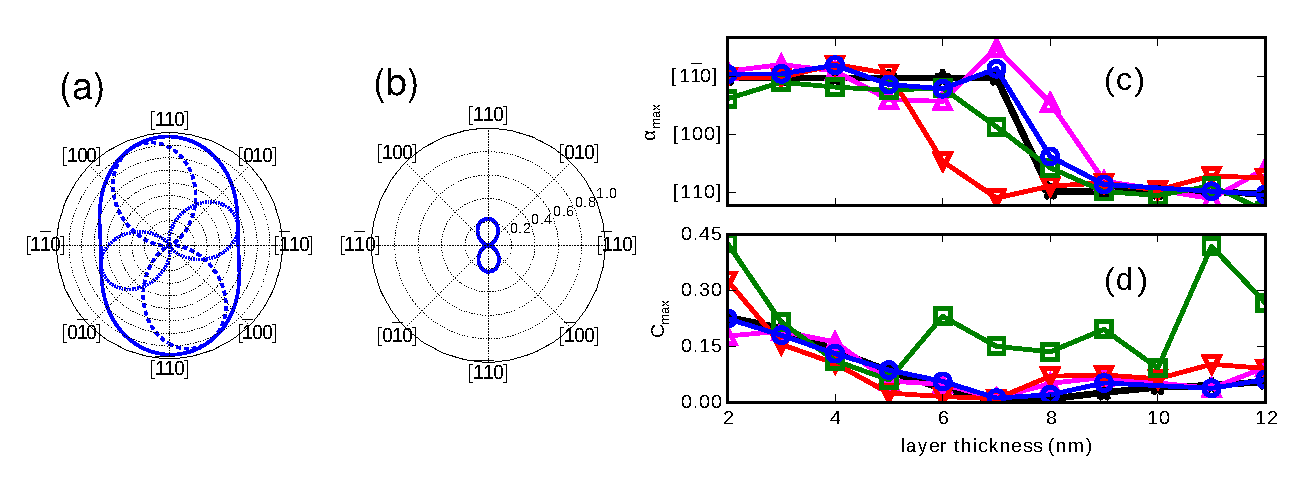
\includegraphics[width=1\linewidth]{/Sci_rep/test/a}
%	\caption{test}
%	\label{fig:kt_sectext}
%\end{figure}

%\newpage 





\section{Theory}

The Taylor expansion of ${\bf P}$ in terms of $\eta$ is obtained as
%
\begin{equation}
\label{eq:2ndPiezGeneral}
P_{\mu}=\sum_je_{\mu j}\eta_j+\frac{1}{2}\sum_{jk}B_{\mu jk}\eta_j\eta_k+\dots,
\end{equation}
%
where $e_{\mu j}$ is the linear and $B_{\mu jk}$ are the quadratic piezoelectric coefficients. In $\mathrm{III-V}$ zincblende semiconductors most of $e$ and $B$ coefficients are equal to each other and only one linear ($e_{14}$) and three non-linear ($B_{114}$, $B_{124}$, $B_{156}$) terms remain independent in Eq.~(\ref{eq:2ndPiezGeneral})~\cite{Beya-Wakata2011}. It is then convenient to rewrite Eq.~(\ref{eq:2ndPiezGeneral}) as ${\bf P}={\bf P}_{l}+{\bf P}_{nl}$, where ${\bf P}_{l}$ is the linear term:
%
%
\begin{equation}
\label{eq:1stPiez}
{\bf P}_{l}=e_{14}\begin{pmatrix}\eta_4\\\eta_5\\\eta_6\end{pmatrix},
\end{equation}
%
and ${\bf P}_{nl}$ the nonlinear one:
%
\begin{equation}
\label{eq:2ndPiez}
{\bf P}_{nl}=B_{114}\begin{pmatrix}\eta_1\eta_4\\\eta_2\eta_5\\\eta_3\eta_6\end{pmatrix}+
B_{124}\begin{pmatrix}\eta_4(\eta_2+\eta_3)\\\eta_5(\eta_3+\eta_1)\\\eta_6(\eta_1+\eta_2)\end{pmatrix}+
B_{156}\begin{pmatrix}\eta_5\eta_6\\\eta_4\eta_6\\\eta_4\eta_5\end{pmatrix}.
\end{equation}
%
%
Here $\eta$-s are indexed according to the Voigt notation,~i.~e.,~ $\eta_1=\eta_{xx}$, $\eta_2=\eta_{yy}$, $\eta_3=\eta_{zz}$, $\eta_4=2\eta_{yz}$, $\eta_5=2\eta_{xz}$, $\eta_6=2\eta_{xy}$~\cite{Beya-Wakata2011} where $x,y,z$ denote the crystallographic axes of the conventional cubic unit cell of the zincblende lattice.
%
%$1=xx,2=yy,3=zz,4=yz,5=xz,6=xy$~\cite{Beya-Wakata2011}.
%
Note that even though the coefficients of the expansion into cubic
%higher order 
terms were provided by Tse and colleagues~\cite{Tse2013}, we restrict ourselves to second-order ones here because of the small magnitude of the externally applied stress of only 0.1$\,$\%~\cite{Aberl:17} and, thus, we can describe experimental results obtained by Aberl~et~al.~\cite{Aberl:17} accurately within this restriction. 


\section{Single-particle calculations based on 8-band $\bf{k \cdot p}$ method}




%Before we present the results of full electronic structure calculations for the InGaAs QDs obtained by the nextnano$^3$ simulation suite~\cite{Birner:07}, we analyze the additional piezoelectric polarization established by the externally applied stress. In particular, we show that despite the small strains in the InGaAs layer occurring as a consequence of deformation of the piezo actuator bonded to the sample, the established piezo-polarization is dominated by the second order constants $B_{\mu,j,k}$. For simplicity, in this section we treat the InGaAs QD as two-dimensional layer with tetragonal symmetry.  
%


%For comparison to our simplified model, 
%
We have used the envelope function approximation based on 8-band ${\bf k}\cdot{\bf p}$ perturbation method using the nextnano$^3$ simulation suite~\cite{Birner:07}. The simulations can be divided into 4~following~steps:
%
\begin{itemize}
	\item [1.] definition of the simulation structure (shape, material parameters),
	\item[2.] calculations of the strain in the structure by minimization of the elastic energy,
	\item[3.] calculations of the electric field in the structure by solving the Poisson equation and calculation of the piezoelectric field,
	\item[4.] solving the single-electron Schrödinger equation using the envelope function approximation.
\end{itemize}
%
%We have calculated the electronic structure of InGaAs/GaAs QDs with the shape of truncated cones as shown in Fig.~\ref{fig:2order:QDStruct} using the envelope function approximation based on 8-band ${\bf k}\cdot{\bf p}$ perturbation method using the nextnano$^3$ simulation suite~\cite{Birner:07}. 
The calculations include full treatment of the elastic strain field employing the Bir-Pikus hamiltonian~\cite{BirPik}. Piezoelectric fields up to the second order in the strain are included self-consistently. Material parameters used in our simulations are listed in Appendix~\ref{app:material_params}. 





We have simulated two structures of InGaAs/GaAs QDs with the shapes of truncated cones that we call QD$_1$ and QD$_2$ differing in size and In alloy distribution.
%
\begin{figure}[!ht]
	\renewcommand{\tabcolsep}{2pt}
	\begin{center}
		\begin{tabular}{c}
			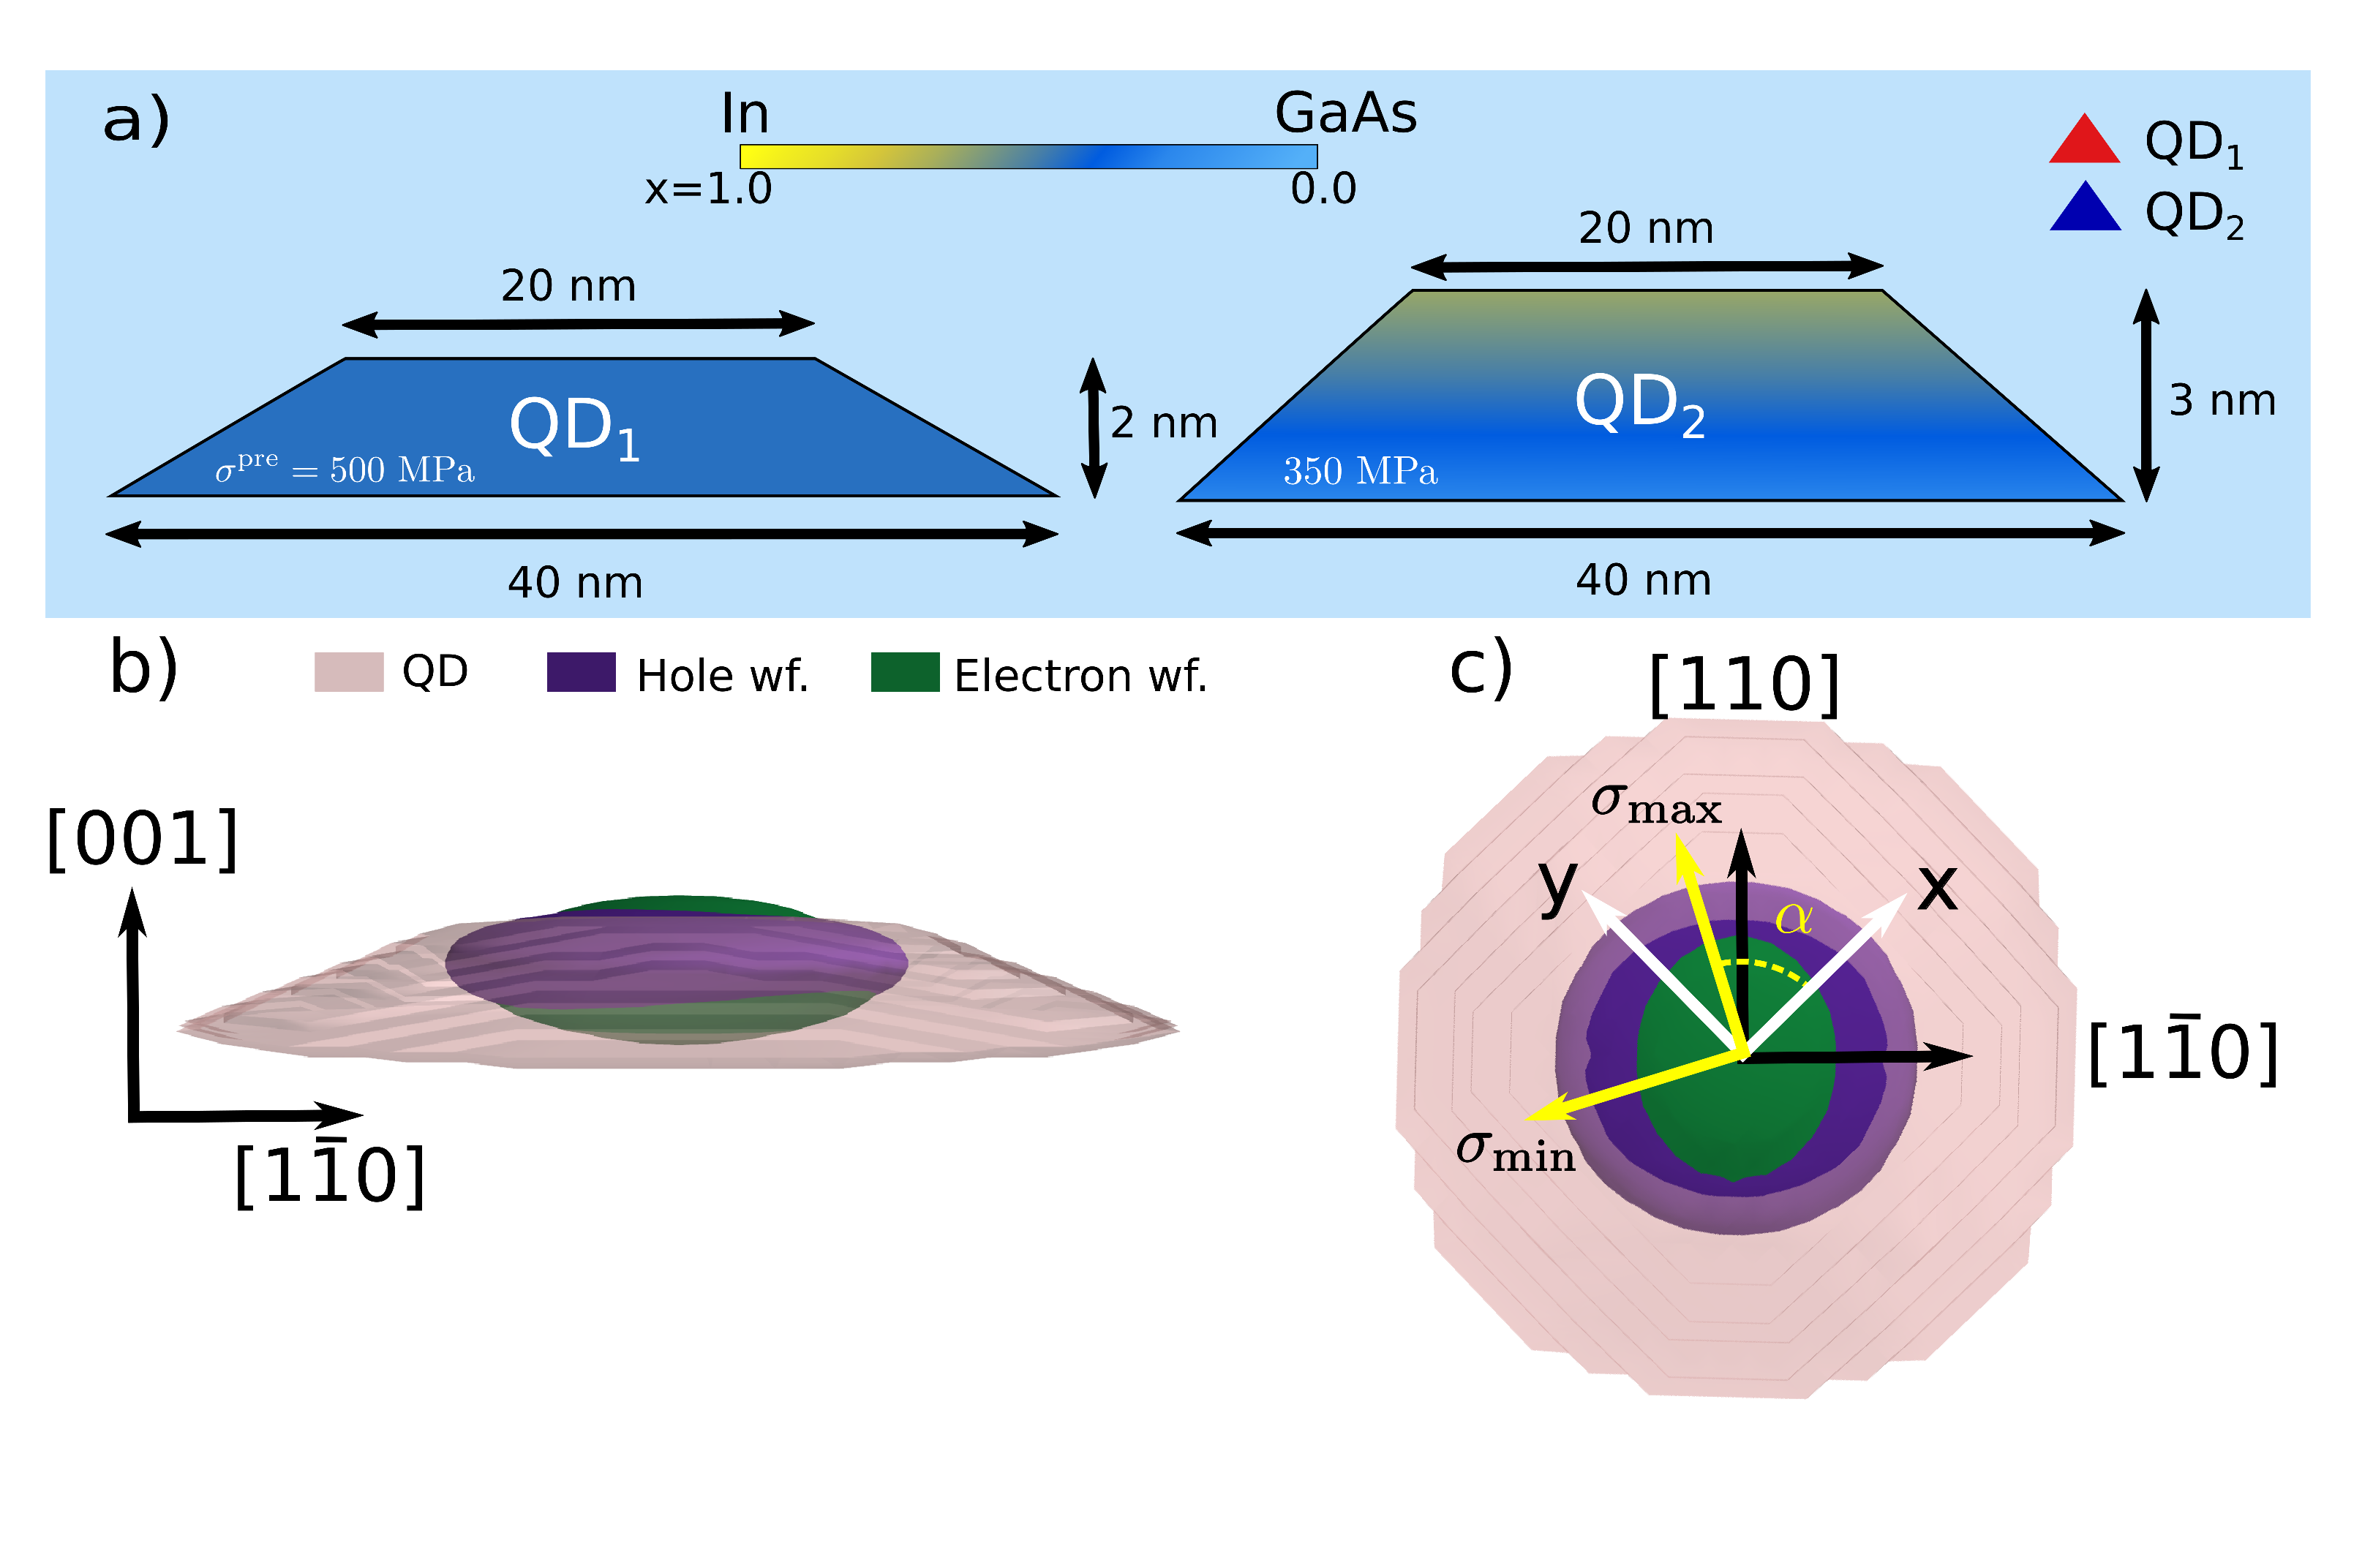
\includegraphics[width=0.8\textwidth]{2_order/180204_structura_wo-gradient_w_triangles_and_wfuncions_vs5} \\ 
		\end{tabular}
	\end{center}
	\caption{In panel a) we show the side view of the calculated In$_{{x}}$Ga$_{1-x}$As/GaAs QD$_1$ and QD$_2$ structures. Both QDs have the shape of truncated cones with base and top diameters of 40$\,$nm and 20$\,$nm, respectively, the height is 2$\,$nm~(3$\,$nm), In composition is constant of 0.45 (linearly increasing from 0.25 at the bottom to 0.65 at the apex), and $\sigma^\text{pre}=500$$\,$MPa ($\sigma^\text{pre}=350$$\,$MPa) for QD$_1$ (QD$_2$). Panels b) and c) show the side and top view, respectively, of the typical simulated dot (pink), and calculated electron (green) and hole (blue) probability densities. The wavefunctions are given as isosurfaces encircling 70\% of the total probability.
		\label{fig:2order:QDStruct}}
\end{figure}

Side views of QD$_1$ and QD$_2$ are shown in Fig.~\ref{fig:2order:QDStruct}~a) and their parameters were deliberately chosen so that the calculated dependencies of the emission energy $E_0$ and of the dipole moment $p$ on the hydrostatic part of the applied anisotropic stress $\sigma_{\mathrm{max}}+\sigma_{\mathrm{min}}$ match the experimental results taken from Ref.~\cite{Aberl:17}, see Fig.~\ref{fig:TheorVsExp}. The variables $\sigma_{\mathrm{max}}$ and $\sigma_{\mathrm{min}}$ denote the principal stresses~\cite{Trotta:15} applied externally by the two-dimensional piezo actuator. In  Ref.~\citep{Aberl:17} it was shown that $\sigma_{\mathrm{max}}$ was applied at an angle of $\alpha=55\,^{\circ}$ with respect to the crystal axis [100], resulting in the principal axis system of the externally applied stress as shown in Fig. \ref{fig:2order:QDStruct}. The various coordinate systems used in our model as well as the single-particle wavefunctions of electrons and holes are indicated in Fig. \ref{fig:2order:QDStruct} b) and c). The connection between the Cartesian and the principal stresses is derived in~Appendix~\ref{app:principal_stress}.

As discussed in Ref.~\cite{Aberl:17}, in course of bonding the sample onto the piezo actuator, a~shear prestess $\sigma^\text{pre}$ independent on the voltage applied to the piezo is exerted on the sample. Consequently, in order to match the measured values of $p$ with results of our calculations we needed to allow for different magnitude of $\sigma^\text{pre}$ of 500 and 350$\,$MPa that acted on QD$_1$ and QD$_2$, respectively.

Experimentally acquired dependencies of $p/e$ on $\sigma_{\mathrm{max}}+\sigma_{\mathrm{min}}$ shown in Fig.~\ref{fig:TheorVsExp} follow a linear behavior, therefore, we have fitted the (gray) data by linear model derived by {Kle\-no\-vský~et~al.}~\cite{Klenovsky_2018_InGaAs_straintuned}
%
\begin{eqnarray}
p/e\approx A^{\mathrm{QD}}\left(\sigma_\mathrm{max}+\sigma_\mathrm{min}\right)+b, \label{eq:strain_model}
\end{eqnarray}
%
which allows us to describe the evolution of $p/e$ by two constants $A^{\mathrm{QD}}$ and $b$. Results of the fit by model~(\ref{eq:strain_model}) are listed in Tab.~\ref{tab:exp_slopes} in Appendix~\ref{app:slopes_of_dipole}.

%


\begin{figure}[!ht]
	\centering
	\renewcommand{\tabcolsep}{2pt}
	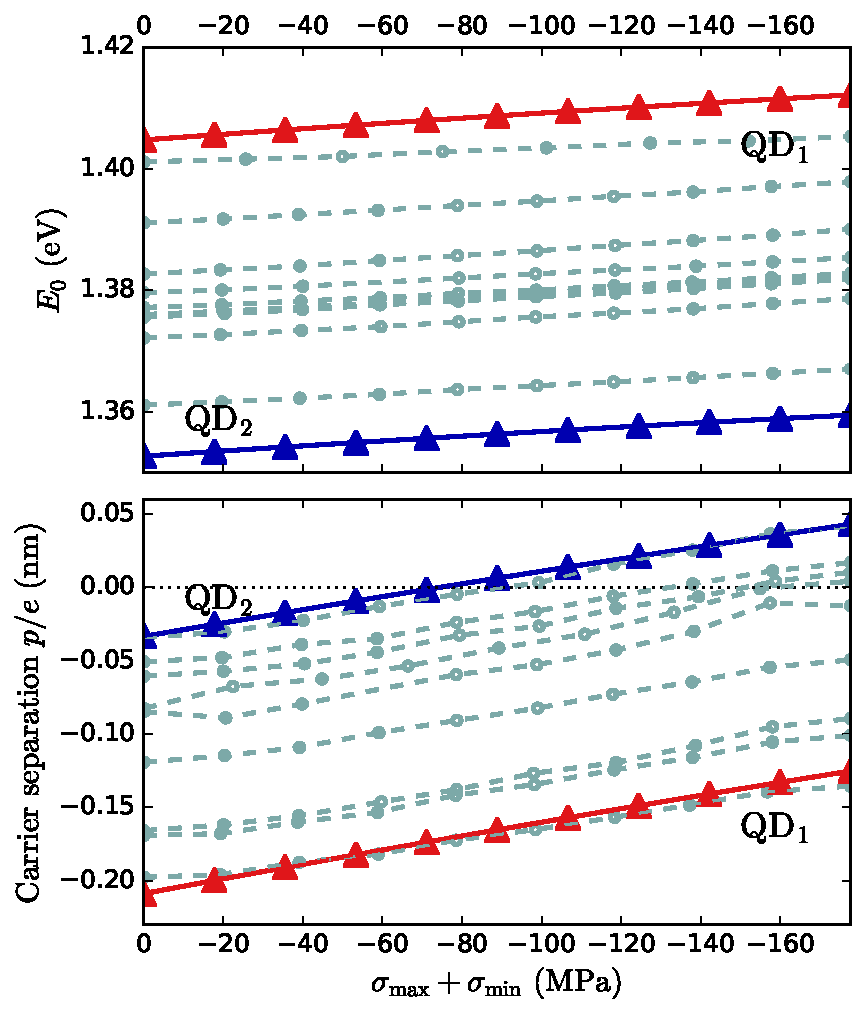
\includegraphics[width=0.5\textwidth]{/2_order/Energy/2018-04-25__171219_8x8_neotocena_++_nn+_35deg_pres500___theoryVSexperiment} 
	\caption{
		Dependencies of $E_0$ (top panel) and $p/e$ (bottom panel) on $\sigma_{\mathrm{max}}+\sigma_{\mathrm{min}}$ experimentally obtained from $\mu$PL measurements of nine InGaAs QDs~\cite{Aberl:17} (dashed curves) and that calculated for QD$_1$ (full red curve) and QD$_2$ (full blue curve). The letter $e$ denotes the elementary charge.}
	%
	%two different QDs, i.e. first with base and top diameter of 30~nm and 15~nm, respectively and height of 3~nm. 
	\label{fig:TheorVsExp}
\end{figure}

\newpage

\section{Effect of second order of piezoelectricity}
%
\begin{figure}[h]
	%\renewcommand{\tabcolsep}{2pt}
	\begin{center}
		\begin{tabular}{cc}
			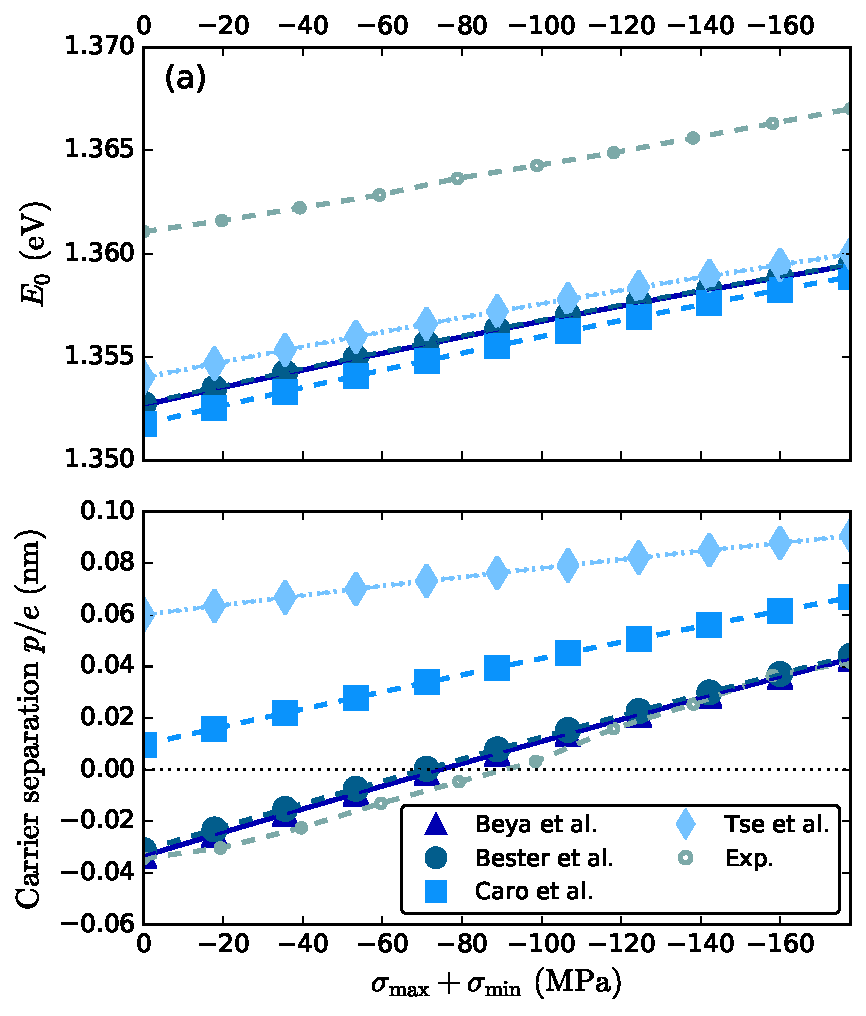
\includegraphics[width=0.5\textwidth]{/2_order/Energy/FINAL_a__171219_8x8_neotocena_++_nn+_35deg_pres350___40x20x3-25-65_350_piezo2ndorder} & 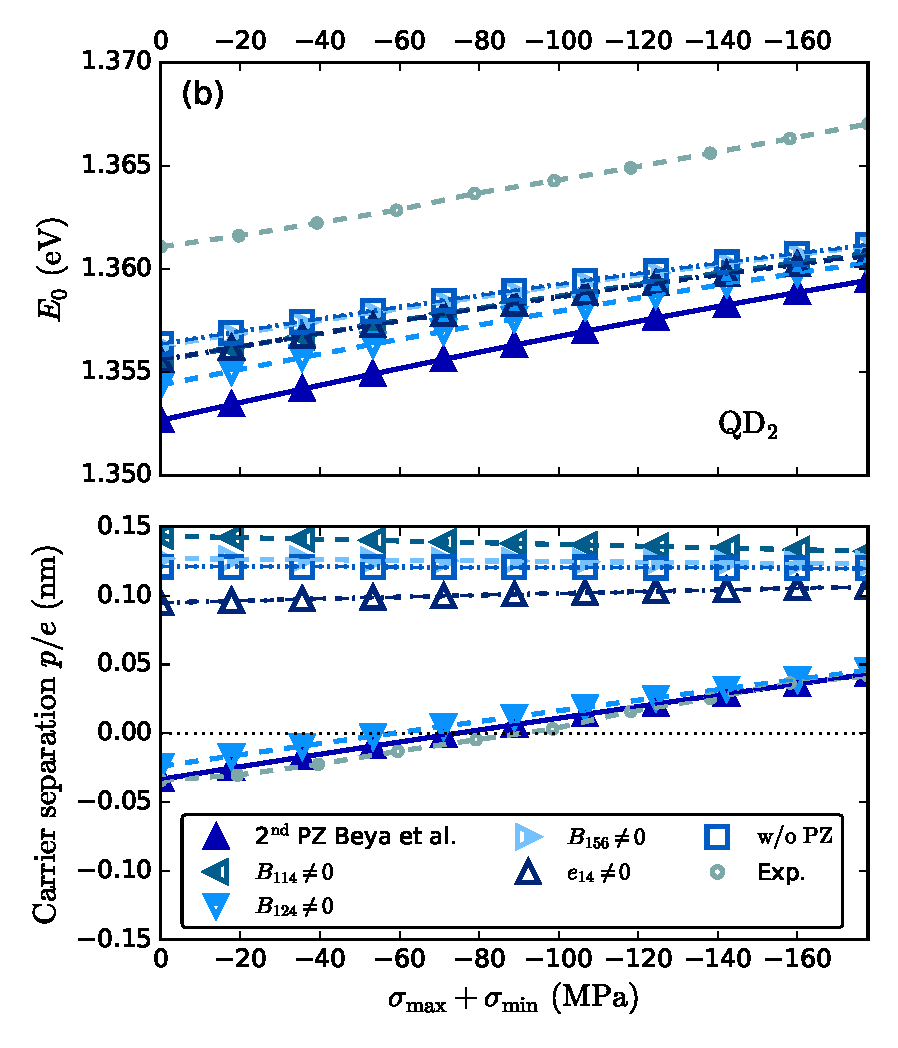
\includegraphics[width=0.5\textwidth]{/2_order/Energy/FINAL_b__171219_8x8_neotocena_++_nn+_35deg_pres350___40x20x3d0_piezo2ndorder_jednotlive_cleny}\\
		\end{tabular}
	\end{center}
	\caption{
		(a) Comparison of calculated results based on four published sets of parameters of second order piezoelectric coefficients, i.~e., Refs.~\cite{Beya-Wakata2011,Bester:06,Caro2015,Tse2013} for QD$_2$. (b) Comparison of dependencies of $E_0$ and $p/e$ on $\sigma_{\mathrm{max}}+\sigma_{\mathrm{min}}$ for all piezoelectric parameters equal to zero except for $e_{14}$, $B_{114}$, $B_{124}$, and $B_{156}$ sequentially retaining their values for QD$_2$. In both (a) and (b) we show the dependencies of $E_0$ on applied stress $\sigma_{\mathrm{max}}+\sigma_{\mathrm{min}}$ in the upper panels and that for $p/e$ in lower ones. 
		The experimental data from Ref.~\cite{Aberl:17} are shown by the grey dashed curves in all panels. 
		\label{fig:DiffPiezo}}
\end{figure}


In Ref.~\cite{Aberl:17} it was discussed that the experimentally obtained values of the dependence of $p/e$ on $\sigma_{\mathrm{max}}+\sigma_{\mathrm{min}}$ can be explained only by including the second-order contribution to the piezoelectric field.
%
Motivated by that, we proceed with the analysis of the evolution of $p/e$ on $\sigma_{\mathrm{max}}+\sigma_{\mathrm{min}}$ for all published second-order piezoelectric parameters listed in Tab.~\ref{tab:second_piez_param}. 
%
%
\begin{table*}[!ht]
	\begin{center}
		\caption{Values for the linear and quadratic piezoelectric coefficients $e_{14}$, $B_{114}$, $B_{124}$ and $B_{156}$. The references from which the parameters were taken are identified in the first column. The units of presented piezoelectric constants are $C/m^2$. For In$_x$Ga$_{1-x}$As, the constants were obtained by linear interpolation.
		\label{tab:second_piez_param}	
		}
		\begin{tabular}{c|ccccc}
			\hline \hline
			%Ref. & compound & $e_{14}$ $(C/m^2)$& $B_{114}$ $(C/m^2)$ & $B_{124}$ $(C/m^2)$&$B_{156}$ $(C/m^2)$\\
			Ref. & compound & $e_{14}$ & $B_{114}$  & $B_{124}$ &$B_{156}$\\
			\hline
			\multirow{2}{*}{Beya-Wakata et al.~\cite{Beya-Wakata2011}} & GaAs & $-0.238$ & $-0.4$  & $-3.8$& $-0.7$\\
			& InAs& $-0.115$ & $-0.6$  & $-4.1$& $0.2$\\
			% 
			\hline
			\multirow{2}{*}{Bester et al.~\cite{Bester:06} }& GaAs & $-0.23$ & $-0.439$  & $-3.765$& $-0.492$\\
			& InAs& $-0.115$ & $-0.531$  & $-4.076$& $-0.12$\\
			%
			\hline
			\multirow{2}{*}{Caro et al.~\cite{Caro2015}} & GaAs & $-0.205$ & $-0.99$  & $-3.21$& $-1.28$\\
			& InAs& $-0.111$ & $-1.17$  & $-4.31$& $-0.46$\\
			%		
			\hline
			\multirow{2}{*}{Tse et al.~\cite{Tse2013}} & GaAs & $-0.16$ & $-0.666$  & $-1.646$& $-$\\
			& InAs& $-0.045$ & $-0.653$  & $-1.617$& $-$\\
			\hline \hline
		\end{tabular}
	\end{center}
\end{table*}
%
%
The results for QD$_2$ are shown in Fig.~\ref{fig:DiffPiezo}~(a) and demonstrate that both the evolution of $p/e$ with $\sigma_{\mathrm{max}}+\sigma_{\mathrm{min}}$ as well as the slopes $\frac{1}{e}\partial p/\partial(\sigma_{\mathrm{max}}+\sigma_{\mathrm{min}})$ and $\partial E_0/\partial(\sigma_{\mathrm{max}}+\sigma_{\mathrm{min}})$ remain remarkably similar among various parameter sets in the literature even though the coefficients differ considerably among them.
For example, the parameter $B_{156}$ has even a different sign between Refs.~\cite{Bester:06} and~\cite{Beya-Wakata2011} or is omitted in Ref.~\cite{Tse2013}.
%


%
%\begin{figure}
%	\begin{center}
	%	\includegraphics[width=0.42\textwidth]{/2_order/FINAL__171219_8x8_neotocena_++_nn+_35deg_pres350___40x20x3d0_piezo2ndorder_jednotlive_cleny}
	%\end{center}
	%\caption{
	%	Comparison of dependencies of $E_0$ and $p/e$ on $\sigma_{\mathrm{max}}+\sigma_{\mathrm{min}}$ for all piezoelectric parameters equal to zero except for $e_{14}$, $B_{114}$, $B_{124}$, and $B_{156}$ sequentially retaining their values for QD$_2$. For comparison, one set of the experimental data from Ref.~\cite{Aberl:17} is given by the grey dashed curve. Otherwise the outline of the figure is the same as that in Fig.~\ref{fig:DiffPiezo}.
	%	\label{fig:DiffPiezoCoeff}}
%\end{figure}


To investigate the origin of that apparent similarity we have performed calculations, in which we have set all piezoelectric parameters equal to zero except for $e_{14}$, $B_{114}$, $B_{124}$, and $B_{156}$ sequentially retaining their values, see Fig.~\ref{fig:DiffPiezo}~(b) for those results for QD$_2$. 


Firstly, we note that the dependencies for $E_0$ are very similar irrespective of which piezoelectric parameter is not set to zero. This is connected with the fact that a change of the emission energy from QDs with stress is dominated by the hydrostatic components.

Secondly, the most important piezoelectric parameter is noticeably $B_{124}$. Evidently, the second term in Eq.~(\ref{eq:2ndPiez}) dominates the dependencies of $E_0$ and $p/e$ on $\sigma_{\mathrm{max}}+\sigma_{\mathrm{min}}$. This is not surprising since the magnitude of $B_{124}$ is several times larger than that of $e_{14}$, $B_{114}$, or $B_{156}$~\cite{Beya-Wakata2011}, see Tab.~\ref{tab:second_piez_param}. 


\section{Effect of indium distribution}

\begin{figure}[!ht]
	\renewcommand{\tabcolsep}{2pt}
	\begin{center}
		\begin{tabular}{c}
			%\includegraphics[width=0.4\textwidth]{2017-12-15__170921_35deg_pres200___30x15x3_concentration.eps} \\
			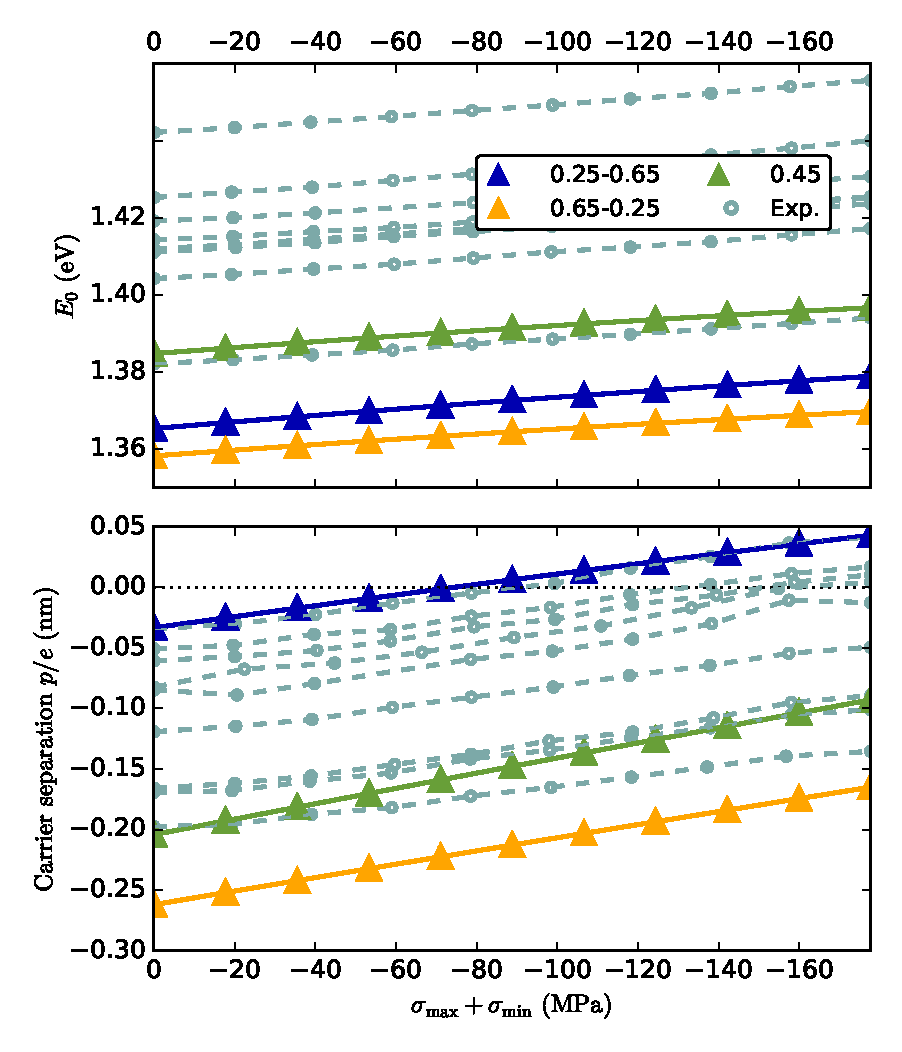
\includegraphics[width=0.5\textwidth]{/2_order/Energy/FINAL__171219_8x8_neotocena_++_nn+_35deg_pres350___40x20x3_concentration} \\
		\end{tabular}
	\end{center}
	\caption{
		Dependencies of $E_0$ (top panel) and $p/e$ (bottom panel) on $\sigma_{\mathrm{max}}+\sigma_{\mathrm{min}}$ experimentally obtained from $\mu$PL measurements of nine InGaAs QDs~\cite{Aberl:17} (dashed curves) and that calculated for different In contents inside QD. The data for In content linearly varying as a function of vertical dimension from 0.25~(0.65) at QD base to 0.65~(0.25) at QD apex are shown as blue~(orange) curves. Those for constant In content of 0.45 are given as green curves. The data calculated assuming second-(first-)order piezoelectricity taken from Ref.~\citep{Beya-Wakata2011} are given as full (open) symbols. All other properties of the dots were the same as for QD$_2$. The letter $e$ denotes the elementary charge.
		\label{fig:TuningByConc}}
\end{figure}
%

Motivated by Refs.~\cite{Grundmann, Fry:00} discussing the influence of indium distribution inside {InGaAs/GaAs} QDs on $p$ we have also studied the effect of that in our stress-tuned dots. In Fig.~\ref{fig:TuningByConc} we show $E_0$ and $p$ as a function of $\sigma_{\mathrm{max}}+\sigma_{\mathrm{min}}$ for In contents (i) linearly increasing from 0.25 at the QD base to 0.65 at its apex, (ii) the same but for reverted concentration profile and (iii) for constant In composition of 0.45. Clearly, we find that $p/e$ where $e$ is the elementary charge at $\sigma_{\mathrm{max}}+\sigma_{\mathrm{min}}=0$ can be varied considerably by changing the slope of In content from $-0.03$$\,$nm for (i) to $-0.26$$\,$nm for (ii). The case (iii) is found in between at $-0.20$$\,$nm. Note that previous values were obtained assuming the second-order piezoelectricity. The data calculated with only first-order piezoelectricity show similar trends in agreement with the results of Refs.~\cite{Grundmann, Fry:00}. Noticeably, both $E_0$ and $\partial E_0/\partial(\sigma_{\mathrm{max}}+\sigma_{\mathrm{min}})$ do not depend appreciably on In distribution and only the mean value of In concentration is important.

However, the slopes $\frac{1}{e}\partial p/\partial(\sigma_{\mathrm{max}}+\sigma_{\mathrm{min}})$ differ considerably in case of first- and second-order piezoelectricity. We find the values of the fitted slopes in the former case in the range from 0.074 to 0.1$\,$nm/GPa while for the latter they are between 0.42 and 0.55$\,$nm/GPa. Slopes of the experimental data are between 0.42 and 0.5$\,$nm/GPa. The relative error of all fitted slopes is $\approx 5$$\,$\%, see also Tab.~\ref{tab:conc_slopes} in Appendix~\ref{app:slopes_of_dipole} for the list of all fitted values and their errors. Thus, very good agreement is found between calculations assuming second-order piezoelectricity and experiment rather than for the first-order. % We will return to this point in the following.


\section{Effect of bonding prestress}
\begin{figure}[!ht]
	\renewcommand{\tabcolsep}{2pt}
	\begin{center}
		\begin{tabular}{c}
			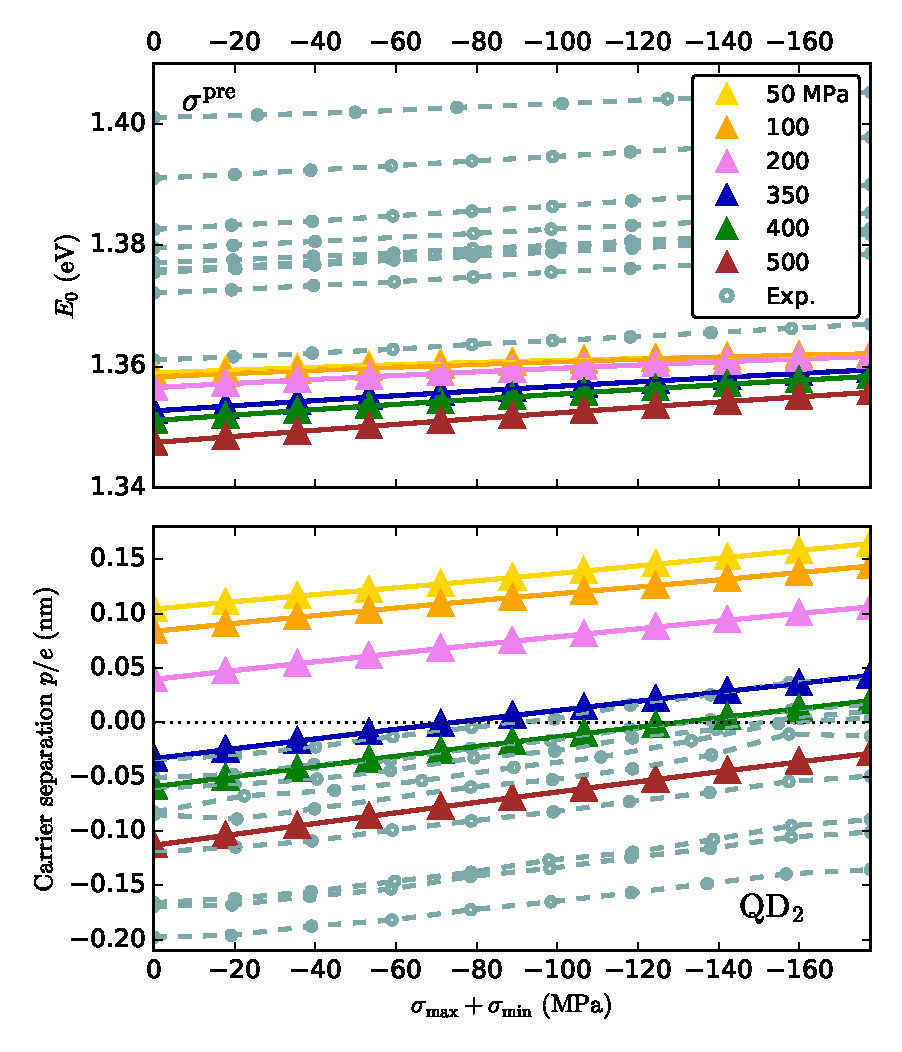
\includegraphics[width=0.5\textwidth]{/2_order/Energy/FINAL__171219_8x8_neotocena_++_nn+_35deg_pres500___prestress} \\
		\end{tabular}
	\end{center}
	\caption{
		Dependencies of $E_0$ (top panel) and $p/e$ (bottom panel) on $\sigma_{\mathrm{max}}+\sigma_{\mathrm{min}}$ experimentally obtained from $\mu$PL measurements of nine InGaAs QDs~\cite{Aberl:17} (dashed curves) and that calculated for different values of $\sigma^{\mathrm{pre}}$. Except for $\sigma^{\mathrm{pre}}$ the simulated QDs had the same properties as QD$_2$. The letter $e$ denotes the elementary charge.
		\label{fig:TuningByPrestress}}
\end{figure}
%
Noticeably, the work in Ref.~\cite{Klenovsky_2018_InGaAs_straintuned} pointed to the importance of prestress $\sigma^\mathrm{pre}$ caused by bonding of the sample onto the piezo actuator. The bonding quality was shown to significantly affect FSS measured during stress-tuning.
%
%, which can be reproduces reas with increasing $\sigma^\mathrm{pre}$. 
%The minimal value 1.15~$\mu$eV of FSS was reached for $\sigma^{\mathrm{pre}}=50$~MPa.




In bottom panel of Fig.~\ref{fig:TuningByPrestress} we show $p/e$ for different values of $\sigma^{\mathrm{pre}}$ acting on QD$_2$. The values of $b$ taken from the fit of dependence of $p/e$ on ${\sigma_{\mathrm{max}}+\sigma_{\mathrm{min}}}$ by linear model~(\ref{eq:strain_model}) decrease with increasing $\sigma^\text{pre}$. Interestingly, $p/e$ attains positive values for  $\sigma^\text{pre}\lesssim 200$$\,$MPa. However, larger values of $\sigma^\text{pre}$ lead to negative values of $p/e$ for $\sigma_{\mathrm{max}}+\sigma_{\mathrm{min}}=0$. 

While $\sigma^{\mathrm{pre}}$ considerably influences the overall magnitude of $p$ it only mildly affects the slope $A^{\mathrm{QD}}$ or the values of $E_0$.
%
%
%

\begin{figure}[!ht]
	\renewcommand{\tabcolsep}{2pt}
	\begin{center}
		\begin{tabular}{c}
			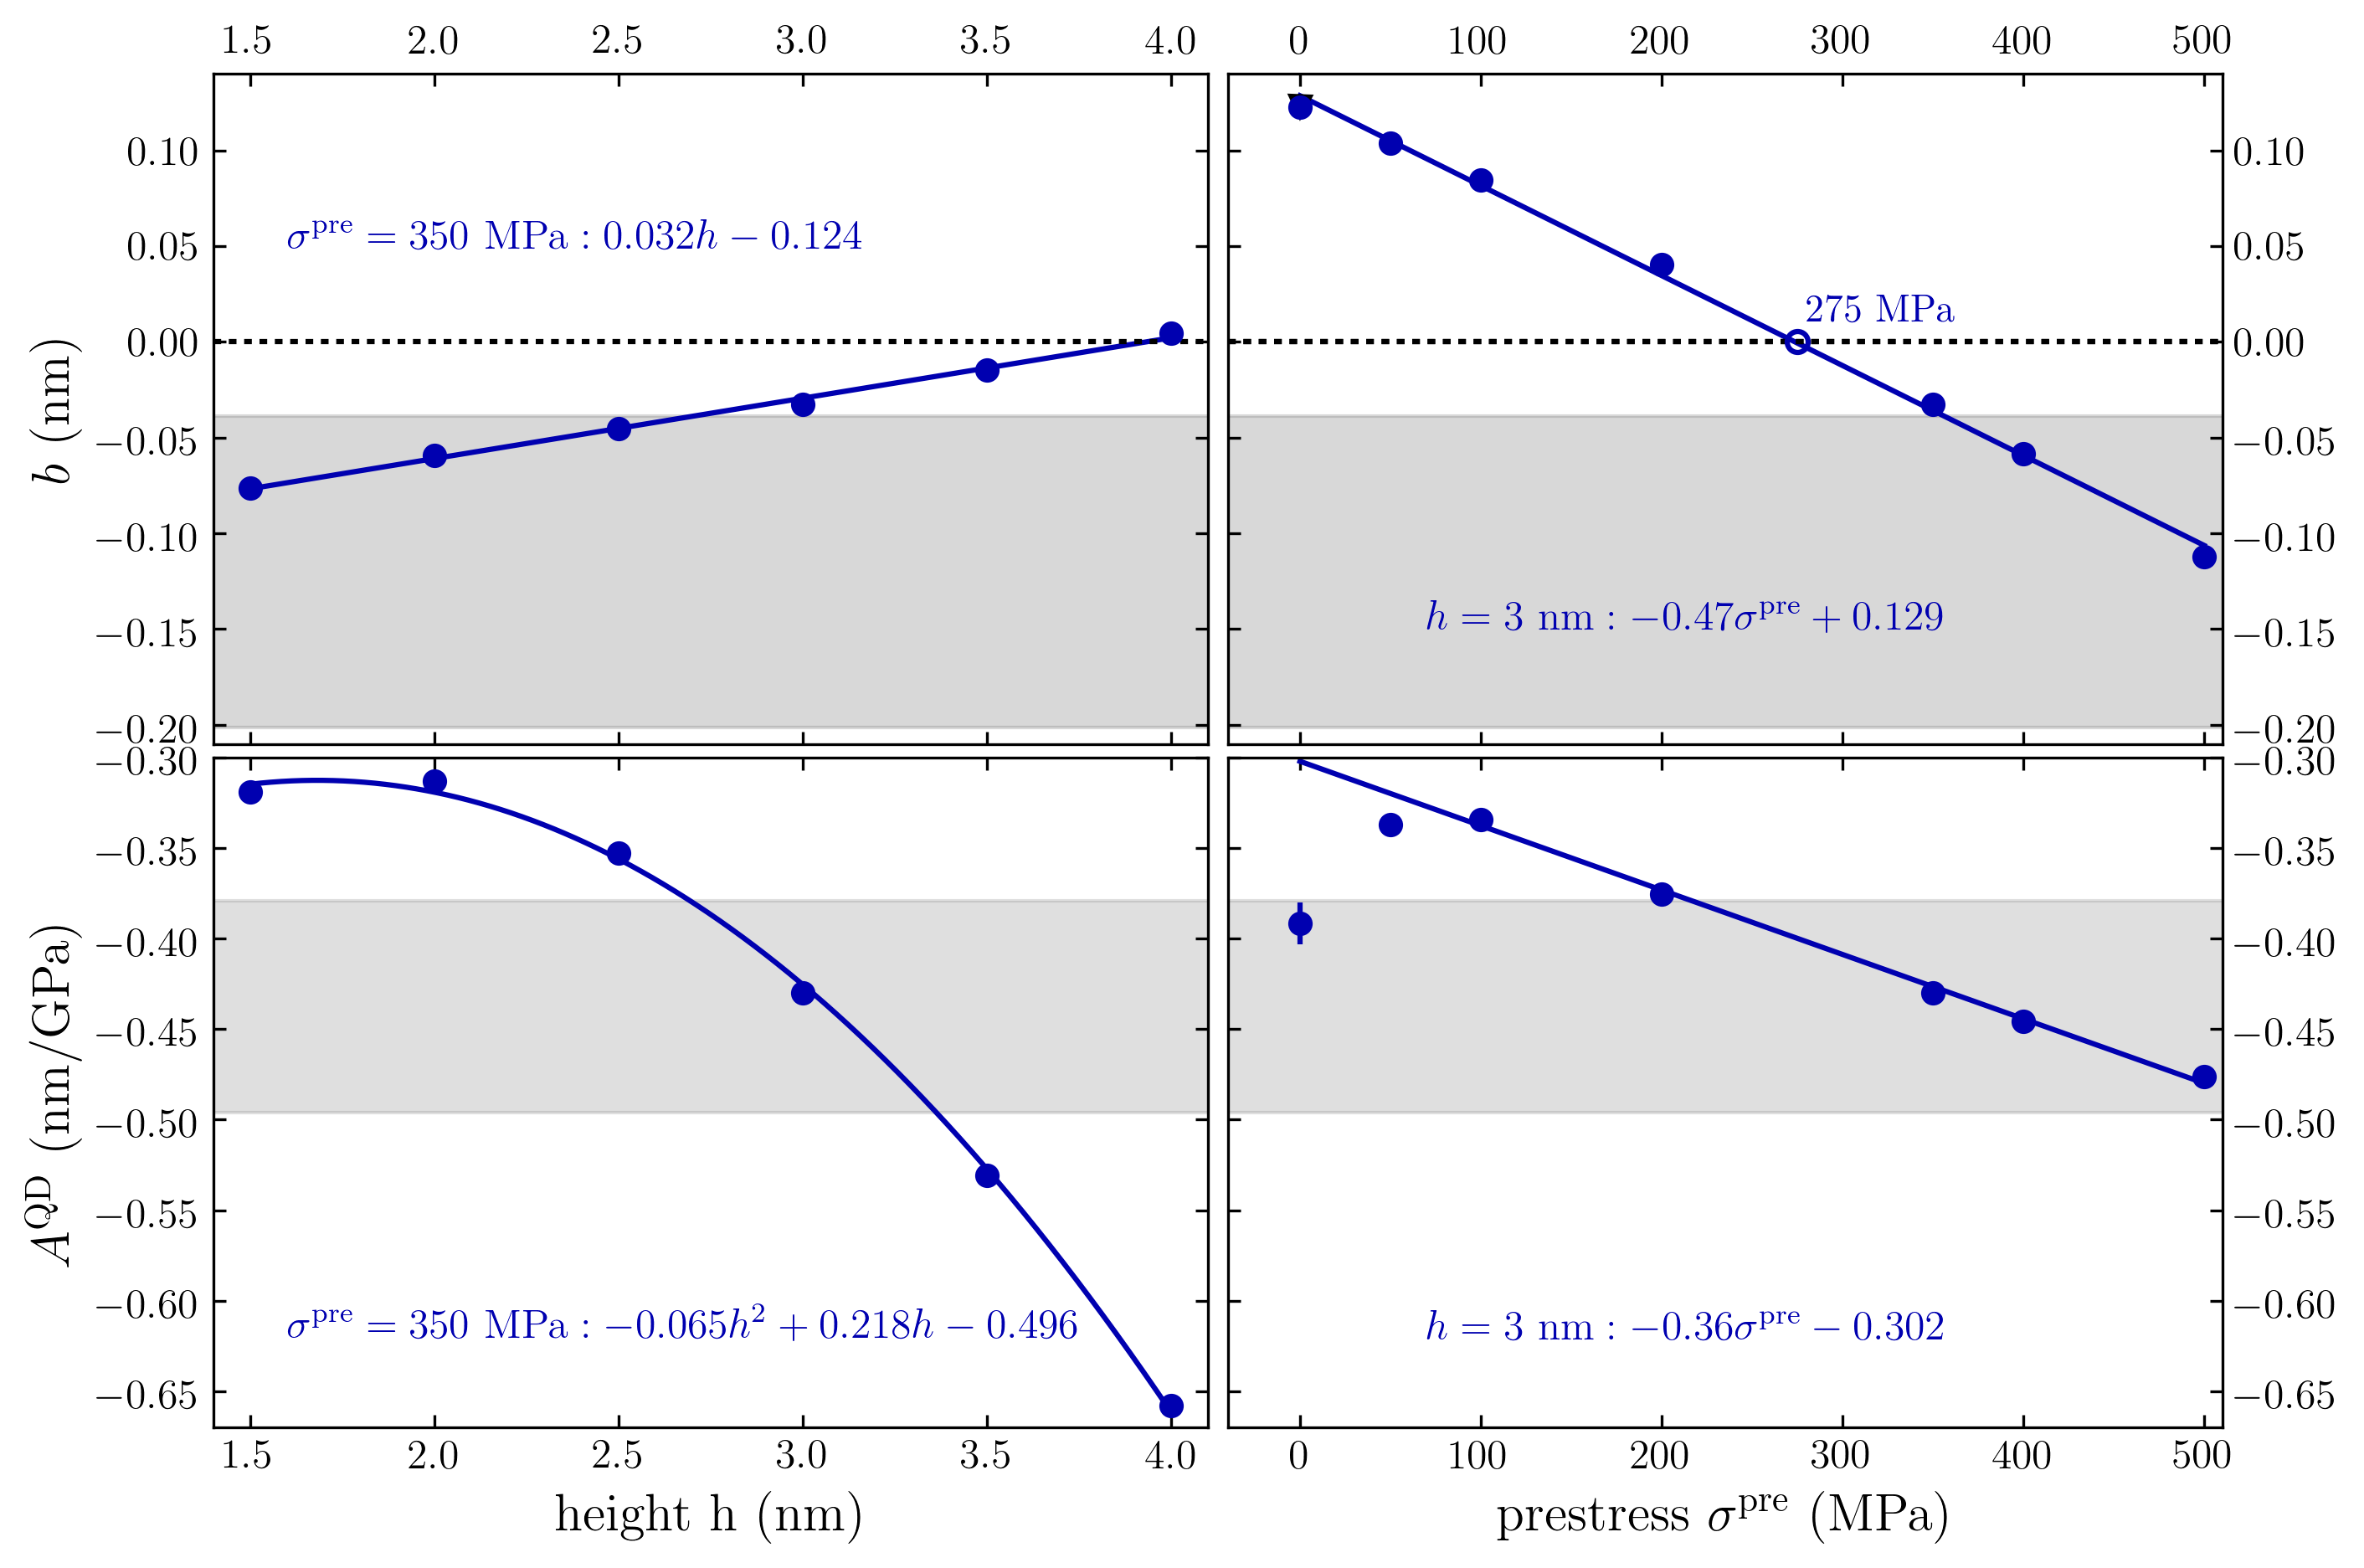
\includegraphics[width=0.9\textwidth]{/2_order/Height_Prestres_fit_pars_3} \\
		\end{tabular}
	\end{center}
	\caption{Evolution of parameters $A^{\mathrm{QD}}$ and $b$ obtained using linear fit $p/e$ on $\sigma_{\mathrm{max}}+\sigma_{\mathrm{min}}$ for varying height of QD (left column) and applied $\sigma^{\mathrm{pre}}$ (right column). Full marks represent values obtained from $\mathbf{k\cdot p}$ calculations, solid lines are fits of the values, and empty symbols point to the values $\sigma^\mathrm{pre}_\mathrm{0}$ where the inversion of $p$ occurs. The grey (yellow) shaded area indicates interval of values observed in $\mu$PL measurements (interval of saturated values of $A^{\mathrm{QD}}$). 
		\label{fig:FitHeightPrestress}}
\end{figure}
%
For a more detailed analysis of the parameters $A^{\mathrm{QD}}$ and $b$ we plot those as a function of $\sigma^{\mathrm{pre}}$ and dot height $h$ and fit them by the linearly decreasing function~(\ref{eq:strain_model}), see resulting parameters in Fig.~\ref{fig:FitHeightPrestress}. The fitted values of the linear model are added in Appendix~\ref{app:empirical_model} in Tab.~\ref{tab:prestress_fit}.

The parameter $b$ can be expressed as a sum of two contributions
\begin{eqnarray}
b =\frac{1}{e} \left(p^\mathrm{pre} + p^\mathrm{QD}\right)=b_1\sigma^\mathrm{pre} +b_0,
\end{eqnarray} 
%
%
where $p^\mathrm{QD}$ is QD dipole without bonding and applied stress, $p^\mathrm{pre}$ is the effect on $p$ of QD created by adding the sample onto the piezo actuator which we assume to be independent on the applied voltage on the piezo~\cite{Aberl:17}. Because $\sigma^{\mathrm{pre}}$ acts against the applied stress $\sigma_{\mathrm{max}}+\sigma_{\mathrm{min}}$ this results in a decrease of $b$ with increasing $\sigma^\mathrm{pre}$. On the other hand, increasing QD height enables the charge carriers to relax more in vertical direction in QD body causing an increase of $b_0=\frac{1}{e}\times p^\mathrm{QD}$. Interestingly, dependencies of $b$ on $\sigma^\mathrm{pre}$ for several QD heights intersect for $\sigma^\mathrm{pre}=500$$\,$MPa.

%
%
Moreover, using the above described approach we can estimate more precisely $\sigma^\mathrm{pre}_\mathrm{0}$ for which the inversion of $p$ occurs. For example, for QD$_2$ we have found $\sigma^\mathrm{pre}_\mathrm{0}=275$$\,$MPa. 
%Interestingly, 
Noticeably, for all dependencies of parameter $A^{\mathrm{QD}}$ on $\sigma^\mathrm{pre}_\mathrm{0}$ we observe an increase in $A^{\mathrm{QD}}$ saturating for some value $\sigma^\mathrm{pre}_\mathrm{c}$, followed again by a linear decrease of $A^{\mathrm{QD}}$, similarly as for the dependencies of $b$. This is a result of using a quadratic dependence of ${\bf P}$ and, thus, $p$ on applied anisotropic stress, see Eq.~(\ref{eq:2ndPiez}).
%
%Unfortunately, so far we have no satisfying physical model of that behavior.

%Similar linear decrease we observe also for $A^{\mathrm{QD}}$ for , .











%








\section{Effect of quantum dot size}

%The emission and dipole moment $p$ of QDs are very sensitive to change not only material composition but also geometrical parameters.
In this section we will focus on tuning of $p$ and $E_0$ by QD height, aspect ratio, or diameter.
%
Firstly, we show the calculations for a set of heights of QD$_2$ in Fig.~\ref{fig:TuningByHeight}. We note that emission energies $E_0$ are smaller for larger heights similarly as in Ref.~\cite{t_schliwa} and can reproduce experimentally obtained $E_0$ in the whole measured range of $\sigma_{\mathrm{max}}+\sigma_{\mathrm{min}}$. Note that the decrease of $E_0$ with increasing QD height is expected since an increase of the latter with other QD parameters set fixed leads effectively to \enquote{widening} of the effective quantum well for quasiparticles in vertical direction.
%
%
\begin{figure}[ht!]
	\renewcommand{\tabcolsep}{2pt}
	\begin{center}
		\begin{tabular}{c}
			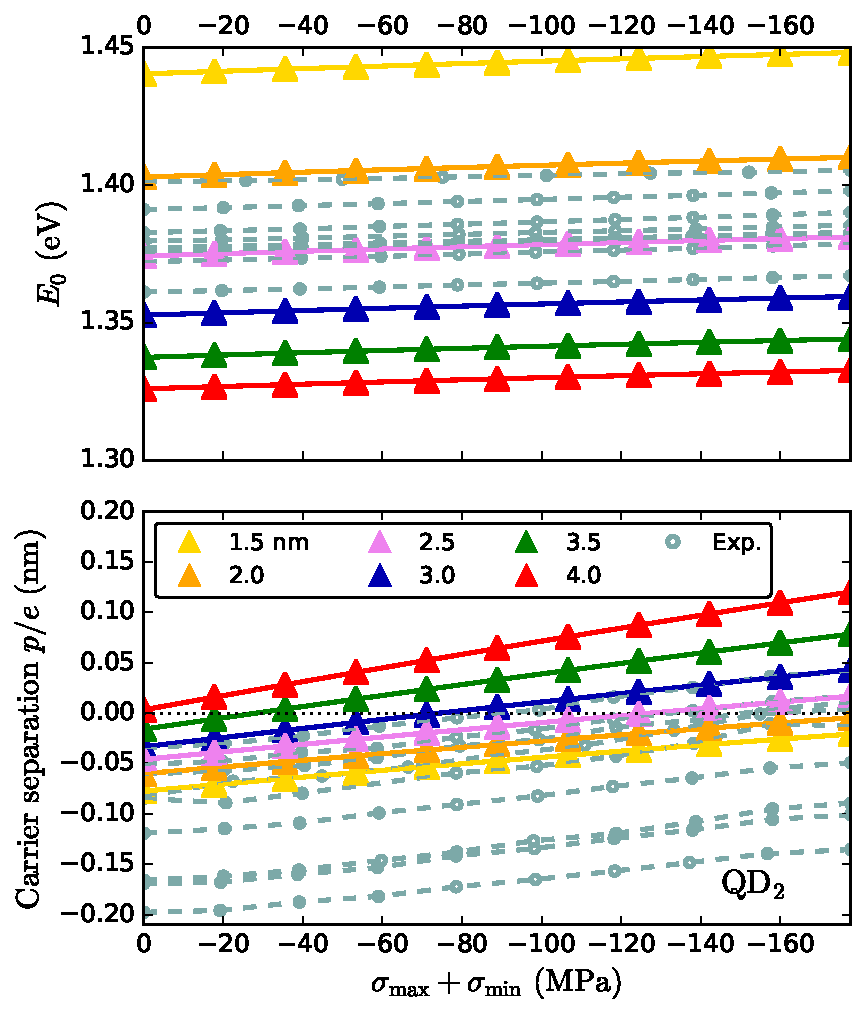
\includegraphics[width=0.5\textwidth]{/2_order/Energy/FINAL__171219_8x8_neotocena_++_nn+_35deg_pres350___40x20_height} \\
		\end{tabular}
	\end{center}
	\caption{
		Dependencies of $E_0$ (top panel) and $p/e$ (bottom panel) on $\sigma_{\mathrm{max}}+\sigma_{\mathrm{min}}$ experimentally obtained from $\mu$PL measurements of nine InGaAs QDs~\cite{Aberl:17} (dashed curves) and that calculated for different values of dot height. Except for height the simulated QDs had the same properties as QD$_2$ including the value of $\sigma^{\mathrm{pre}}=350$$\,$MPa. The letter $e$ denotes the elementary charge.
		\label{fig:TuningByHeight}}
\end{figure}

However, the dot height influences both $A^{\mathrm{QD}}$ and $b$ parameters in the dependency of $p/e$ on $\sigma_{\mathrm{max}}+\sigma_{\mathrm{min}}$. While $b$ is modified only slightly from $-0.076$ to $0.005$$\,$nm when changing $\sigma_{\mathrm{max}}+\sigma_{\mathrm{min}}$ from $-177$ to $0$$\,$MPa, at the same time $A^{\mathrm{QD}}$ increases dramatically from $-0.66$ to $-0.32$.




%
%

%

Finally, in Fig.~\ref{fig:TuningByLateral} we show the effect of variations in the lateral dimensions of QDs. In panel~(a) we change both the diameter of upper and lower plane for a fixed ratio of those, and in panel~(b) we vary the ratio of dimensions of upper and lower plane for fixed diameter of the latter.


%changes of the base top diameters of the QD truncated cone lead to absolute shifts of $E_0$ and $p/e$ but neither lateral dimension nor aspect (ratio between top and base radius) of QD entail variation in slopes of both quantity which is demonstrated in Fig.~\ref{fig:TuningByLateral}.

\begin{figure}[!ht]
	\renewcommand{\tabcolsep}{2pt}
	\begin{center}
		\begin{tabular}{cc}
			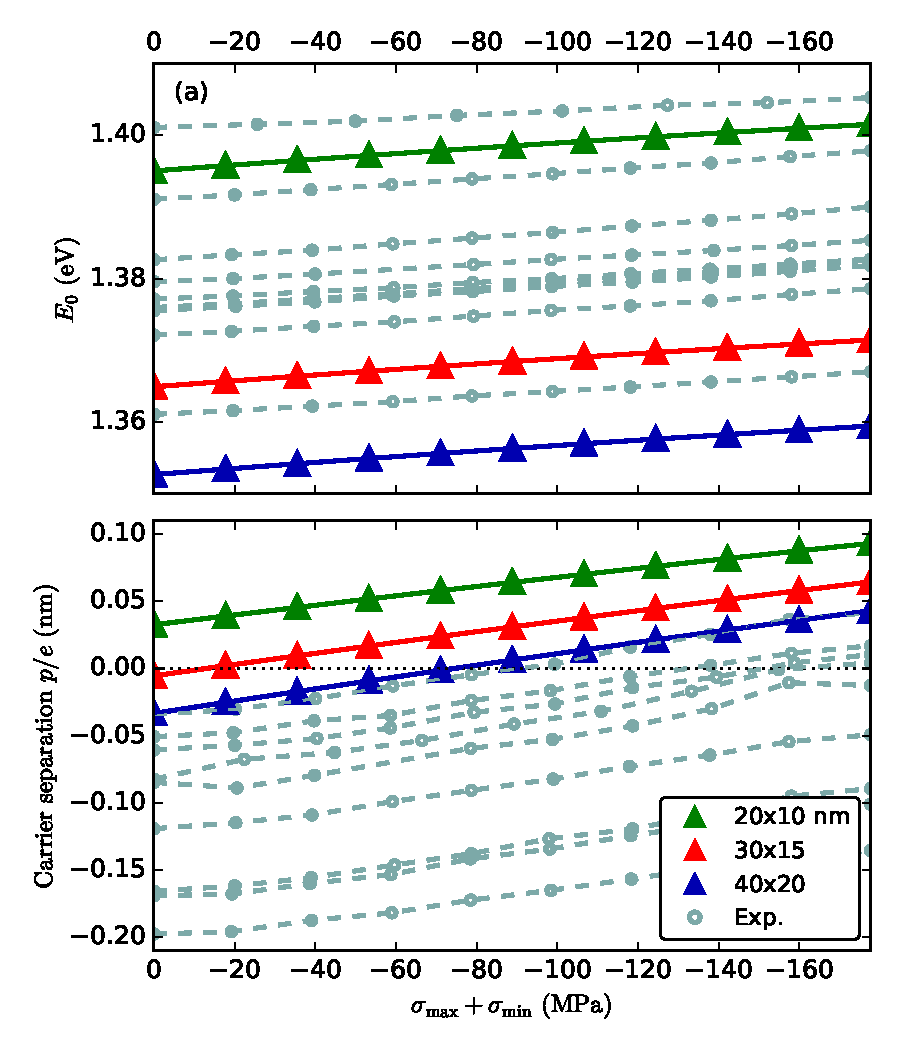
\includegraphics[width=0.5\textwidth]{/2_order/Energy/FINAL__171219_8x8_neotocena_++_nn+_35deg_pres350_h3___lateral} &
			%
			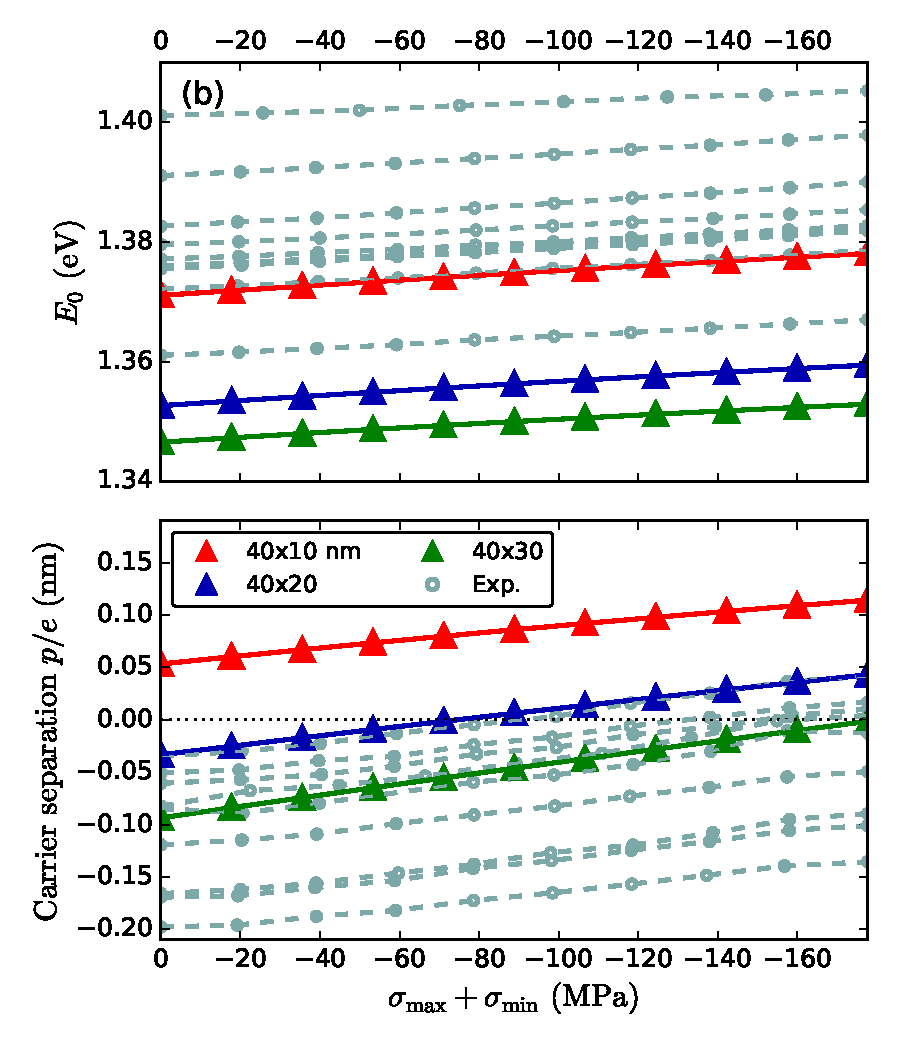
\includegraphics[width=0.5\textwidth]{/2_order/Energy/FINAL__171219_8x8_neotocena_++_nn+_35deg_pres350_h3___aspect} \\
		\end{tabular}
	\end{center}
	\caption{
		Dependencies of $E_0$ (top panels) and $p/e$ (bottom panels) on $\sigma_{\mathrm{max}}+\sigma_{\mathrm{min}}$ experimentally obtained from $\mu$PL measurements of nine InGaAs QDs~\cite{Aberl:17} (dashed curves) and that calculated for different values of (a) dot base diameter with fixed aspect ratio of 1/2 to the diameter of the the upper plane and (b) aspect with fixed base diameter of 40$\,$nm. Except for varied quantities the simulated QDs had the same properties as QD$_2$ including the value of $\sigma^{\mathrm{pre}}=350$$\,$MPa. The letter $e$ denotes the elementary charge.
		\label{fig:TuningByLateral}}
\end{figure}

Because previous analysis has led us to realize that only $\sigma^\mathrm{pre}$ and height are mostly important for tuning of $p$, we repeat similar evaluation as before,~i.~e., plot $A^\mathrm{QD}$ and $b$ as a function of QD height.
%
We can see in left column of Fig.~\ref{fig:FitHeightPrestress} that both $A^\mathrm{QD}$ and $b$ quadratically evolve with dot height. While $A^\mathrm{QD}$ shows similar dependence on height for all studied $\sigma^\mathrm{pre}$, dependence of $b$ on height is changing from convex for small $\sigma^\mathrm{pre}$ 
%(smaller than 500~MPa for QD$_2$) 
to concave for large values of $\sigma^\mathrm{pre}$. 

The latter behavior, in turn, provides comparison of the importance of dot structural properties particularly In alloy profile and $\sigma^{\mathrm{pre}}$ on $p$ for $\sigma_{\mathrm{max}}+\sigma_{\mathrm{min}}=0$. Smaller values of $\sigma^{\mathrm{pre}}$ are insufficient to overcome the effect of In alloy on dipole and, furthermore, for fixed value of $\sigma^{\mathrm{pre}}$ the influence of In alloy on dipole increases even more with QD height, leading to convex dependence. On the other hand, large values of $\sigma^{\mathrm{pre}}$ (in our structure $\sigma^{\mathrm{pre}}>500$$\,$MPa) rather easily overcome the effect of dot composition on dipole which is then mostly controlled only by $\sigma^{\mathrm{pre}}$.

%












\section*{Conclusions}
We have studied the effects of non-linear piezoelectricity on emission energy and electric dipole moment in stress tuned InGaAs/GaAs quantum dots and pinpointed the importance of that for studies of those systems as compared to using first-order terms only. 
%and pinpointed the dominant piezoelectric term. 
Also, we have shown the necessity of the presence of a large built-in in-plane strain due to the lattice mismatch in order for the pronounced changes of the electron-hole dipole to occur as a result of an externally applied stress. 

Furthermore, we have illustrated the use of an effective linear model to find the electric dipole moment in quantum dots as a function of quantum dot height and its build-in prestress. For these quantities we have shown the evolution of parameters from linear fits of the dipole on applied stress. 

Finally in Tab.~\ref{tab:conclusion_straintuned}, we summarize effects of selected parameters on emission energy and electric dipole.

\begin{table*}[ht!]
	\begin{center}
		\caption{Summary of different parameters that we used to tune the emission energy $E_0$ and electric dipole $p$ on the hydrostatic applied stress $\sigma^{\rm{app}}=\sigma_{\mathrm{max}}+\sigma_{\mathrm{min}}$ in stress-tuned InGaAs QDs assuming second-order piezoelectricity. Meaning of symbols is the following: symbol $\textcolor{ps_green}{\boldsymbol{+}}$ ($\textcolor{red}{\boldsymbol{-}}$) indicates increase (decrease) of $E_0$ or $p$ with increasing parameter in the leftmost column.  \label{tab:conclusion_straintuned} 
		}
		\begin{tabular}{c|cc|cc}
			\hline \hline
			\multirow{2}{*}{Dependency on} &  \multicolumn{2}{c|}{Energy} & \multicolumn{2}{c}{Dipole}\\ \cline{2-5}
			 &   $E_0$ & $\partial E_0/\partial\sigma_\mathrm{app}$  & $b$ & $A^{\mathrm{QD}}$\\  \hline
			 %
			 %
			 %2$^\mathrm{nd}$ piezo&   o & $\textcolor{ps_green}{\boldsymbol{+}}$  & o&$\textcolor{red}{\boldsymbol{-}}$\\ \hline
			 %
			  In contribution &  mean & o  & mean &o\\ \hline
			 %
			 $\sigma^\mathrm{pre}$ &  o &  $\textcolor{ps_green}{\boldsymbol{+}}$  & $\textcolor{red}{\boldsymbol{--}}$ &$\textcolor{red}{\boldsymbol{-}}$\\ \hline
			 %
			 Height&  $\textcolor{ps_green}{\boldsymbol{++}}$&  o  & $\textcolor{ps_green}{\boldsymbol{+}}$ &$\textcolor{ps_green}{\boldsymbol{++}}$\\ \hline
			 %
			 Base &  $\textcolor{ps_green}{\boldsymbol{++}}$&  o   &$\textcolor{ps_green}{\boldsymbol{++}}$ & o\\ \hline
			 %
			 Aspect &  $\textcolor{ps_green}{\boldsymbol{++}}$&  o   &$\textcolor{ps_green}{\boldsymbol{++}}$ & o\\ \hline
			 %
			 %
			 %
			 \multicolumn{5}{c}{o no effect \qquad $\textcolor{ps_green}{\boldsymbol{+}}$ increase \qquad $\textcolor{red}{\boldsymbol{-}}$ decrease }\\
			\hline \hline
		\end{tabular}
	\end{center}
\end{table*}



%https://books.google.cz/books?id=DiFMPmXSsLUC&pg=SA6-PA15&lpg=SA6-PA15&dq=Varshni+1967&source=bl&ots=hBJXnBqrHH&sig=WuCbtLj6FUIWMr09BP1LkBR-2cc&hl=cs&sa=X&ved=0ahUKEwi5mPz5lL_ZAhUGEVAKHRiaAOIQ6AEIXDAH#v=onepage&q=Varshni%201967&f=false

\chapter{Excitonic structure and pumping power dependent emission blue-shift of type-II quantum dots}
\label{chap:SciRep}


Semiconductor quantum dots (QDs) are one of the most promising candidate systems for the realization of quantum cryptography protocols~\citep{Muller2014,Strauf2007} or quantum gates~\citep{Stevenson2006,Rodt} in the information technologies. Most of the interest in the literature is focused on type-I QDs with both electron and hole states confined in the QD body. 
However, the spatial separation of the quasiparticle wavefunctions in so-called type-II QDs leads to smaller overlap of the wavefunctions resulting in reduced emission intensity and recombination rate~\citep{Klenovsky10,KleJOPCS,Hsu,Nishikawa2012}. Moreover, a large blue-shift of emission energy with increasing laser pumping has been observed~\citep{Jin,UlloaHomogSRL}. The carrier separation in type-II confined systems has several advantages compared to those of type-I nature. In particular, a naturally small fine-structure splitting (FSS)~\citep{Krapek2015} and molecular-like states~\citep{Klenovsky10,KleJOPCS,KrapekNottingham} were predicted. As a result, type-II QDs might be used in quantum information technology without the need for post-processing of the quantum states. 

There has been only a small number of studies of the excitonic structure of type-II QDs~\citep{Matsuda2007,Miloszewski2014} so far due to their inhomogeneous broadening of the spectral bands. Hence, in this chapter we investigate the multi-particle states by experimental observation of the recombination using intensity and polarization resolved photoluminiscence (PL) measurements of InAs/GaAsSb/GaAs QDs. Our experiment is supported by theoretical description by a Full Configuration Interaction method (CI) developed by the supervisor~\citep{Klenovsky2017}. Finally, we have simulated the experimentally observed blue-shift of the emission of these QDs using a semi-self-consistent CI algorithm~\citep{Klenovsky2017}.

\medskip
For the theoretical description and the experimental testing we have chosen GaAsSb capped InAs QDs in GaAs matrix. This system is favored because it allows continuous change of type confinement by varying Sb content in GaAsSb capping layer (CL)~\citep{Klenovsky10}.

\medskip
In this chapter we present results of theoretical calculations of the multi-particle structure of our system performed by the supervisor, followed by experimental verification of that done by the author of this thesis. Note, that we show here the former mainly as a guide to the experiments.
\newpage 




\section{Multi-excitonic structure calculation} \label{sec:scirep_theory}
The multi-excitonic structure of studied QDs was calculated by the CI method. The single-particle basis states were obtained by the Nextnano++ simulation package~\citep{next} using the envelope function approximation based on the eight-band $\mathbf{k \cdot p}$ method. In distribution in a simulated lens shape InAs QD with height of 4~nm and basis diameter of 16~nm was either constant at 0.6, or trumpet-like. The thickness $d$ and Sb composition of the CL were varied during calculations. 
%
\begin{figure}
	\centering
	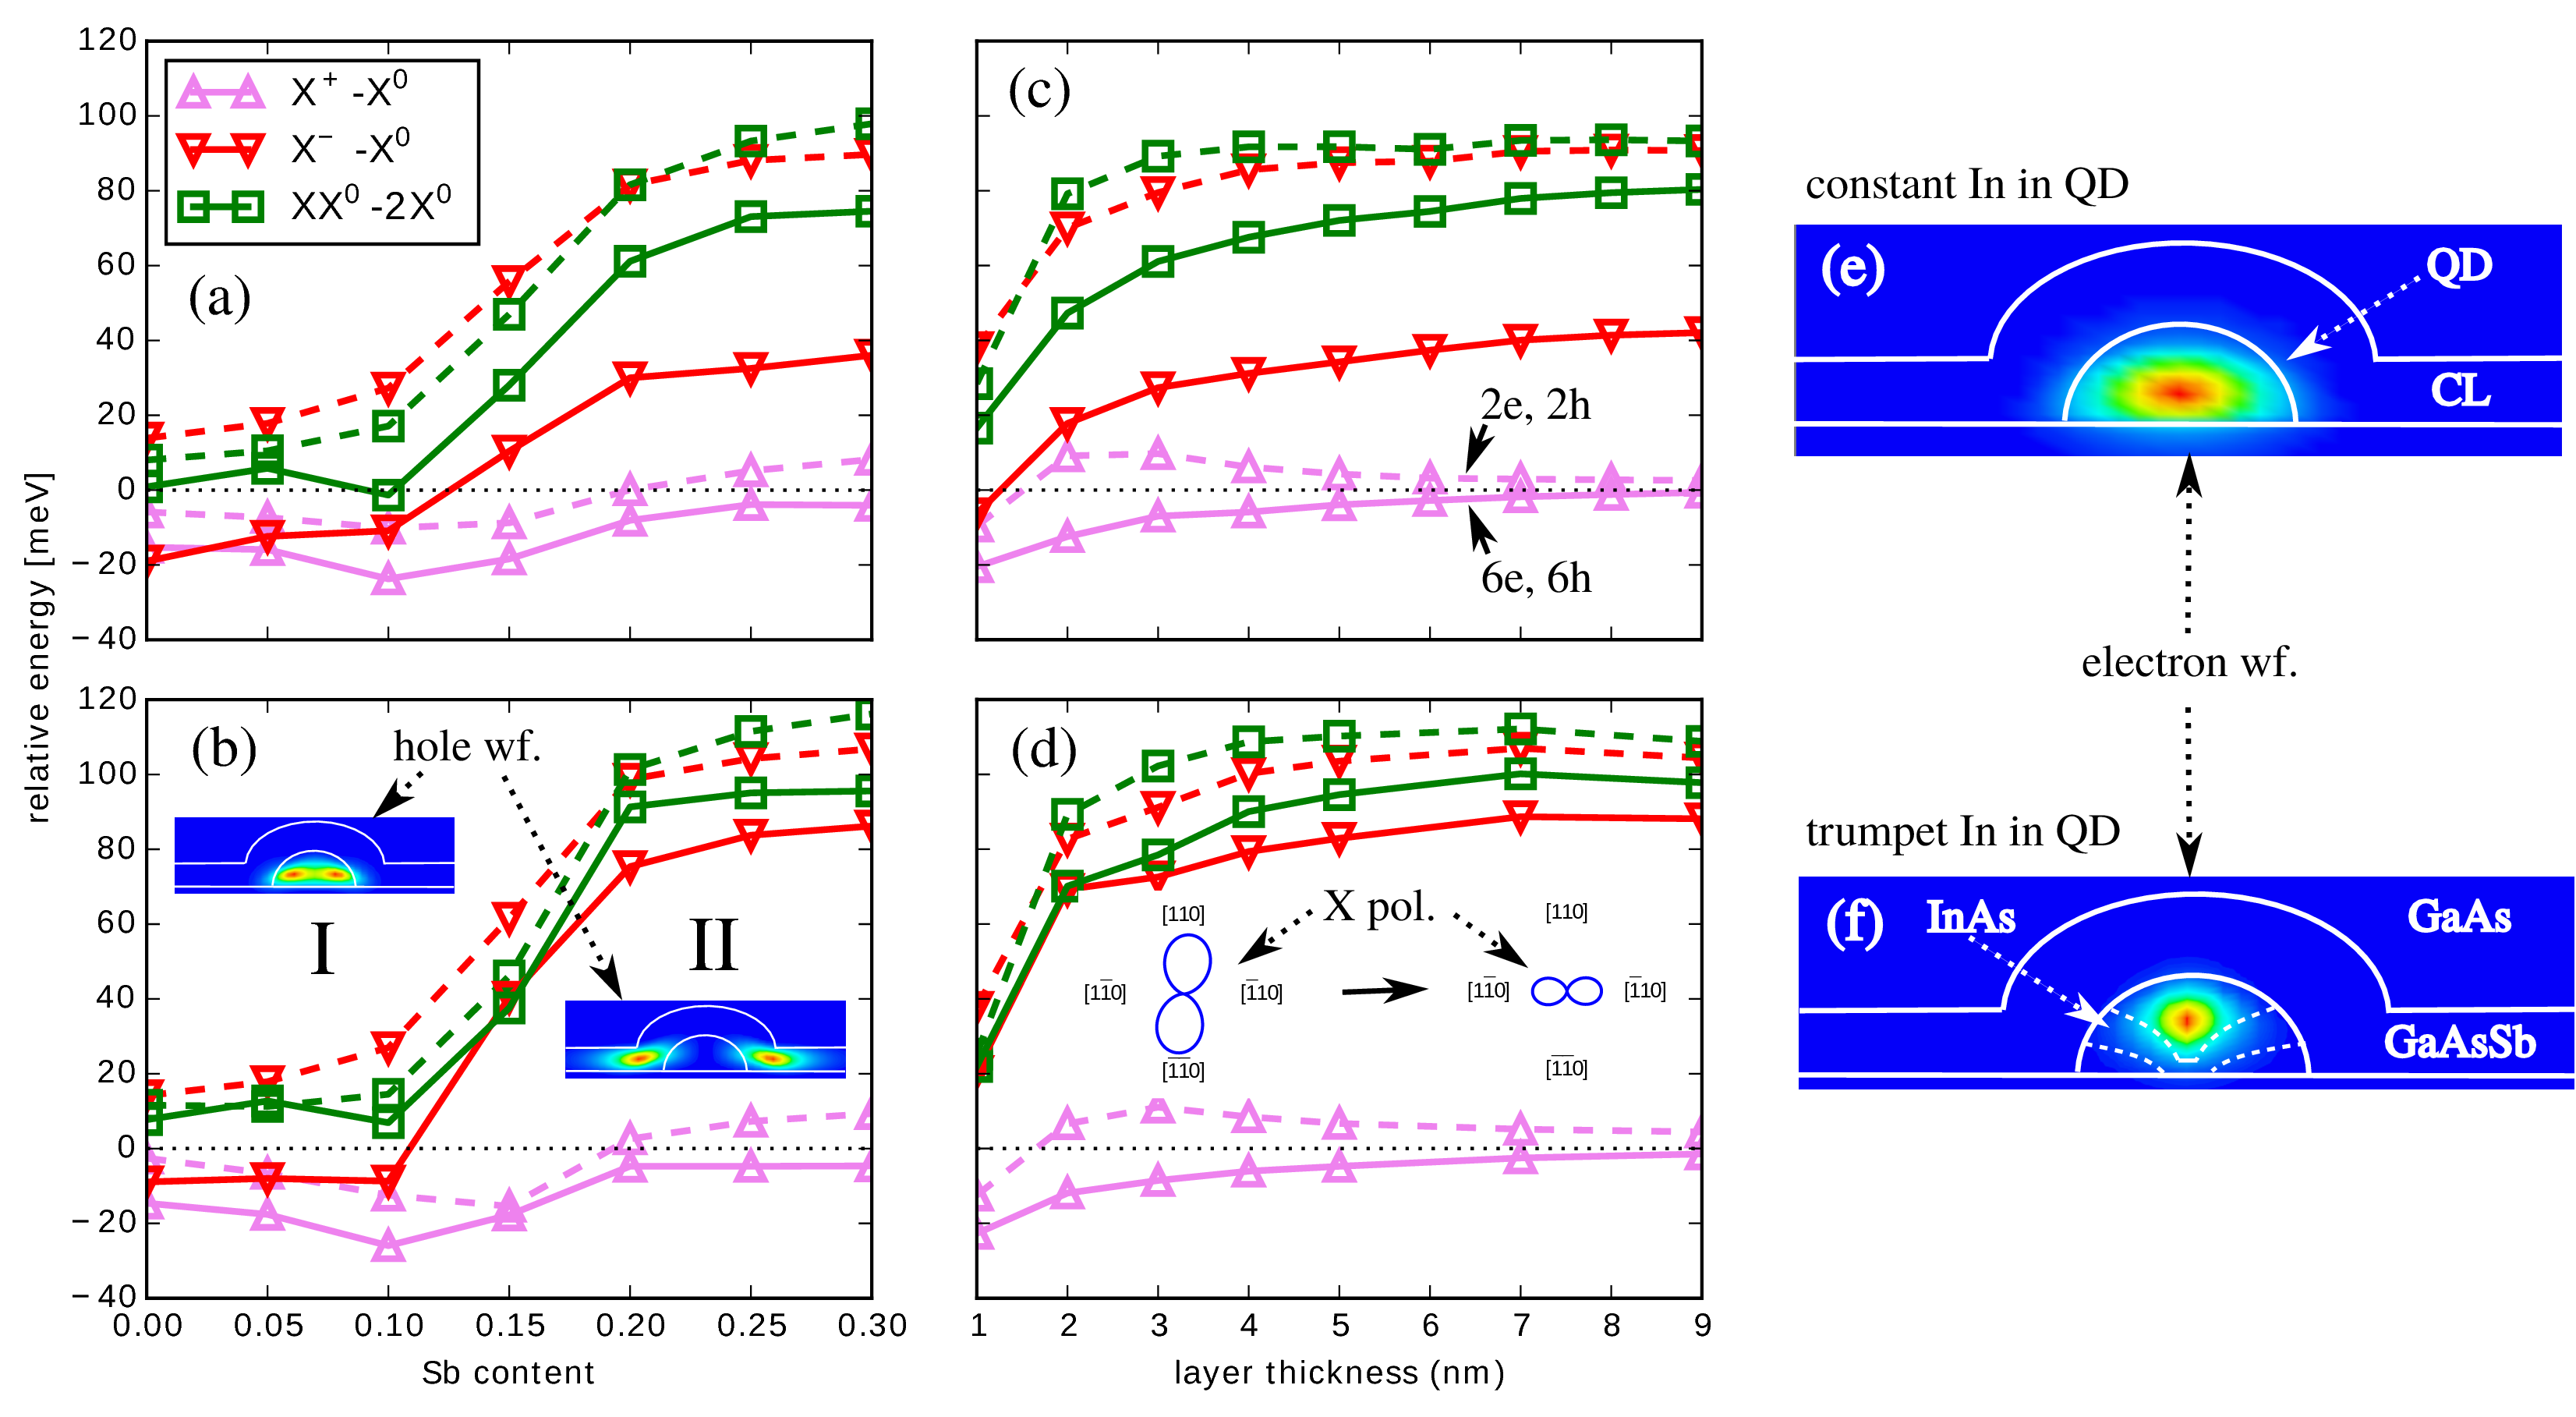
\includegraphics[width=1\linewidth]{/Sci_rep/article/theory}
	\caption{Energies of the complexes $X^+$, $X^-$, and $XX^0$ with respect to that of $X^0$ as functions of (a, b) Sb content for a constant and trumpet In composition in QD with CL thickness $d=5~\mathrm{nm}$, respectively, and (c, d) $d$ for fixed Sb content of 0.24 in the same QDs. The dashed lines show calculations with 2 electron and 2 hole single-particle basis states while the full lines that for 6~by~6 basis. In insets of panel~(b) are $(1\overline{1}0)$~plane cuts of the hole probability densities, and labels I and II represent the type of confinement, respectively. The inset of (d) illustrates the polarization of the emission of $X^0$ for thin and thick CL. Panels (e) and (f) show simulated structures and probability density of the electron wavefunction in QD for constant In content of 0.6 and trumpet In distribution, respectively.}
	\label{fig:Sci_rep_theory}
\end{figure}
%

In Fig.~\ref{fig:Sci_rep_theory}~(a) and (b) we show the calculated Sb content dependencies of the energy differences of $X^+$, $X^-$, and $XX^0$ from $X^0$ for QD with constant In content [panel (a)] and trumpet In composition~\cite{Migliorato} [panel (b)], respectively. It can be seen that transition associated with $X^-$ and $XX^0$ becomes significantly anti-binding in type-II confined structures where holes are located in CL whereas electrons in QD body (see the inset of Fig.~\ref{fig:Sci_rep_theory}~(b) for the hole, and panels (e) and (f) for the electron wavefunctions). However, if CL is too thin the energy of holes is too large for localization of the hole ground state in CL and the type of confinement the system becomes of type-I nature marked by increased value of binding energy of complexes demonstrated for heterostructure with varying $d$ of CL for a fixed Sb content of 0.24 in Fig.~\ref{fig:Sci_rep_theory}~(c) and (d). Moreover, the increase of $d$ leads to a change in the vertical position of the hole wavefunction from the base of QD to above its apex. This is connected with a change in the orientation of the emission polarization and allows the determination of the vertical position of the hole from polarization resolved PL measurements, see Ref.~\citep{Klenovsky2016}. 

The binding energies of $XX^0$ and $X^-$ in type-II are, depending on the calculated dependencies and In distribution, in the range of 60--120~meV and 20--90~meV. On the other hand, in all our simulations $X^+$ remains rather anti-binding, more precisely its binding energy is between -20 and 5~meV. Detailed information about CI method and more detailed analysis of the results can be found in Ref.~\citep{Klenovsky2017}.


\section{InAs/GaAsSb/GaAs QD samples}
%For the theoretical description and the experimental testing have chosen GaAsSb capped InAs QDs in GaAs matrix. This system is favoured because it allows continuous change of type confinement by varying Sb content in GaAsSb capping layer~\citep{Klenovsky10} as can be seen in Fig.~\ref{fig:Sci_rep_theory}(a) and (b), where are the Sb content dependencies of the energy differences of $X^+$, $X^-$ and $XX^0$ from $X^0$ calculated by the supervisor using CI method, for details see Ref.~\citep{Klenovsky2017} or Sec.~\ref{Sec:CI}.

Structures for PL measurements were prepared by AIXTRON~200 with a non-rotating graphite susceptor on GaAs(100) substrate using a low pressure (7~kPa) metal-organic vapour phase epitaxy (MOVPE) in Stranski-Krastanov growth mode at the Institute of Physics of the Czech Academy of Sciences (FZU). First, the temperature was set to 650~$^\circ$C for the growth of the first GaAs buffer layer, then that was reduced to 510~$^\circ$C for the growth of the rest of the structure: (i) 10~nm thick GaAs buffer layer, (ii) 2 monolayers (MLs) of InAs for the growth of QDs, (iii) 5~nm of GaAsSb capping layer (CL) and (iv) 100~nm GaAs finishing layer. Information about used precursors and growth rate can be found in Ref.~\citep{Klenovsky2016}.

For comparison with the measured phenomena of type-II QDs, we examined also type-I InAs/GaAs(001) QDs with a stack of 3 layers of InAs dots grown above each other by MOVPE in Stranski-Krastanov mode. For more information see Ref.~\citep{HumPhysE}.

\section{Photoluminescence setup}
%
\begin{figure}
	\centering
	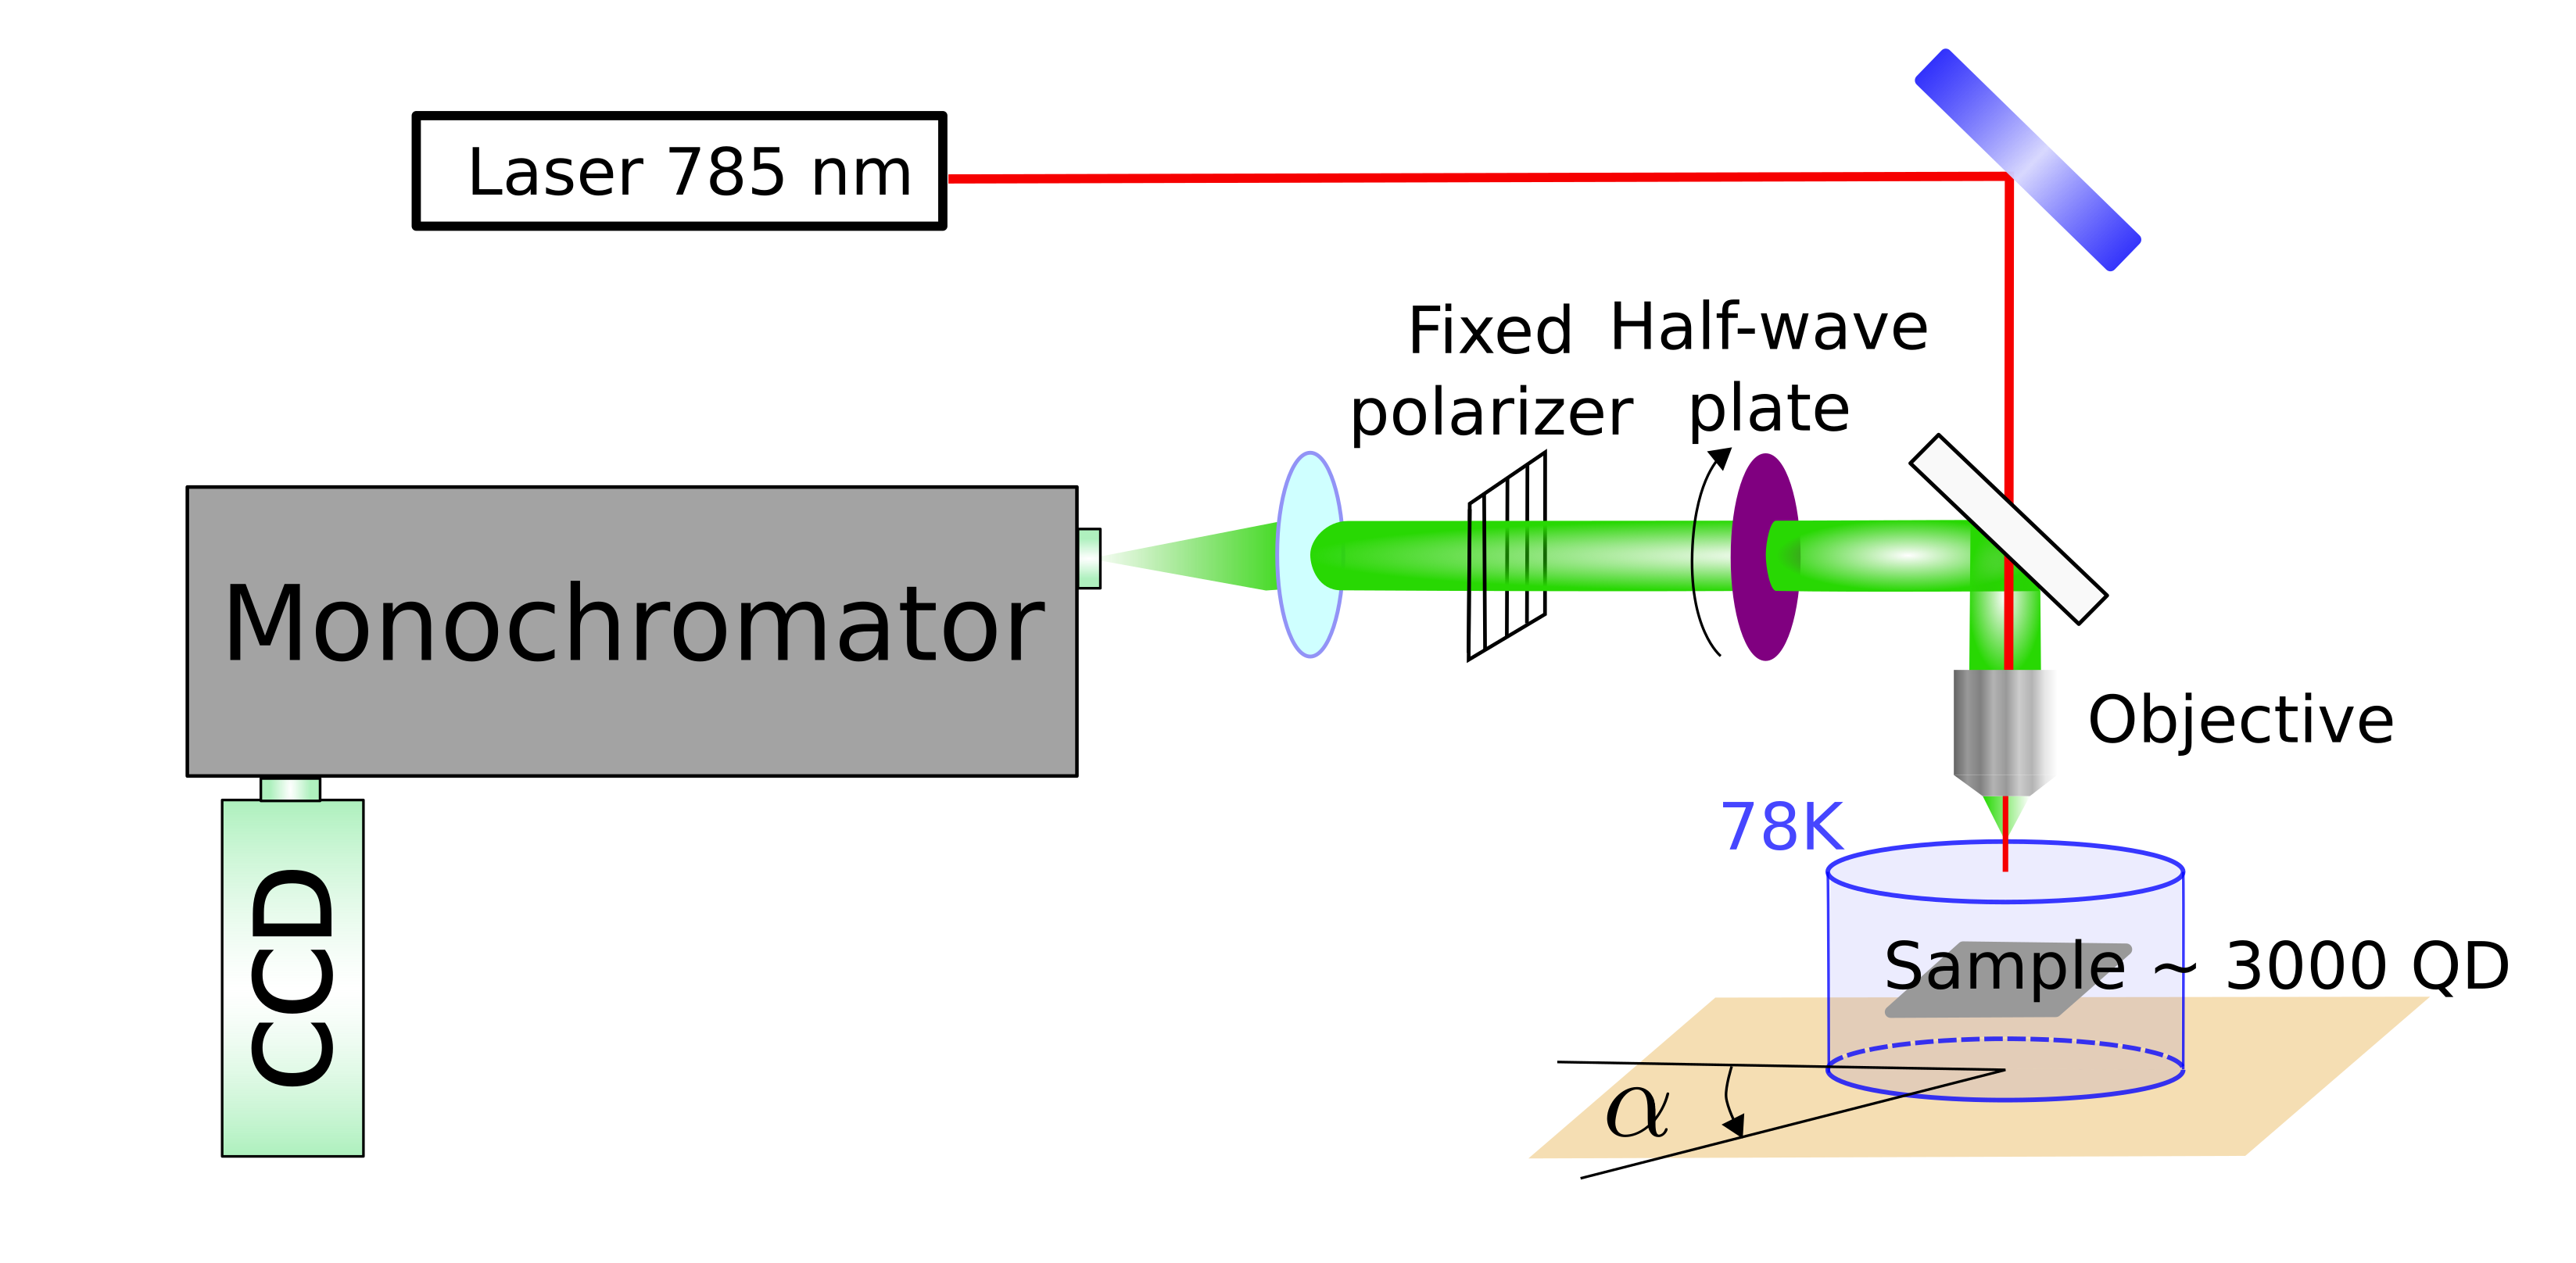
\includegraphics[width=0.9\linewidth]{/Sci_rep/article/setup_scirep}
	\caption{A sketch of the PL setup.}
	\label{fig:}
\end{figure}
The PL measurements were performed using the NT-MDT Ntegra-Spectra spectrometer. The samples were cooled to liquid nitrogen temperature and pumped by a solid-state laser with the emission wavelength of 785~nm. The maximum laser power on the surface was 5~mW focused by lens on 150~$\mu\mathrm{m}^2$ area and laser intensity was varied using a neutral density (ND) filter. 

%
The polarization of the emission spectrum was analyzed by a rotating achromatic half-wave retarder with the maximal transmission at 1300~nm followed by a fixed Glan-Taylor linear polarizer. The PL signal was dispersed by a 150~grooves/mm ruled grating and detected by the InGaAs line-CCD camera, cooled to minus 90~$^\circ$C to reduce thermal noise. In every experiment, PL signal was collected from a large number of QDs ($\sim$3000). Because the transmission of the setup depends on the photon energy, we have eliminated this effect by calibration to blackbody emission. 


The efficiency of the InGaAs CCD camera and emission spectrum of calibration source are depicted in Fig.~\ref{fig:calib_scirep}.
\begin{figure}
	\centering
	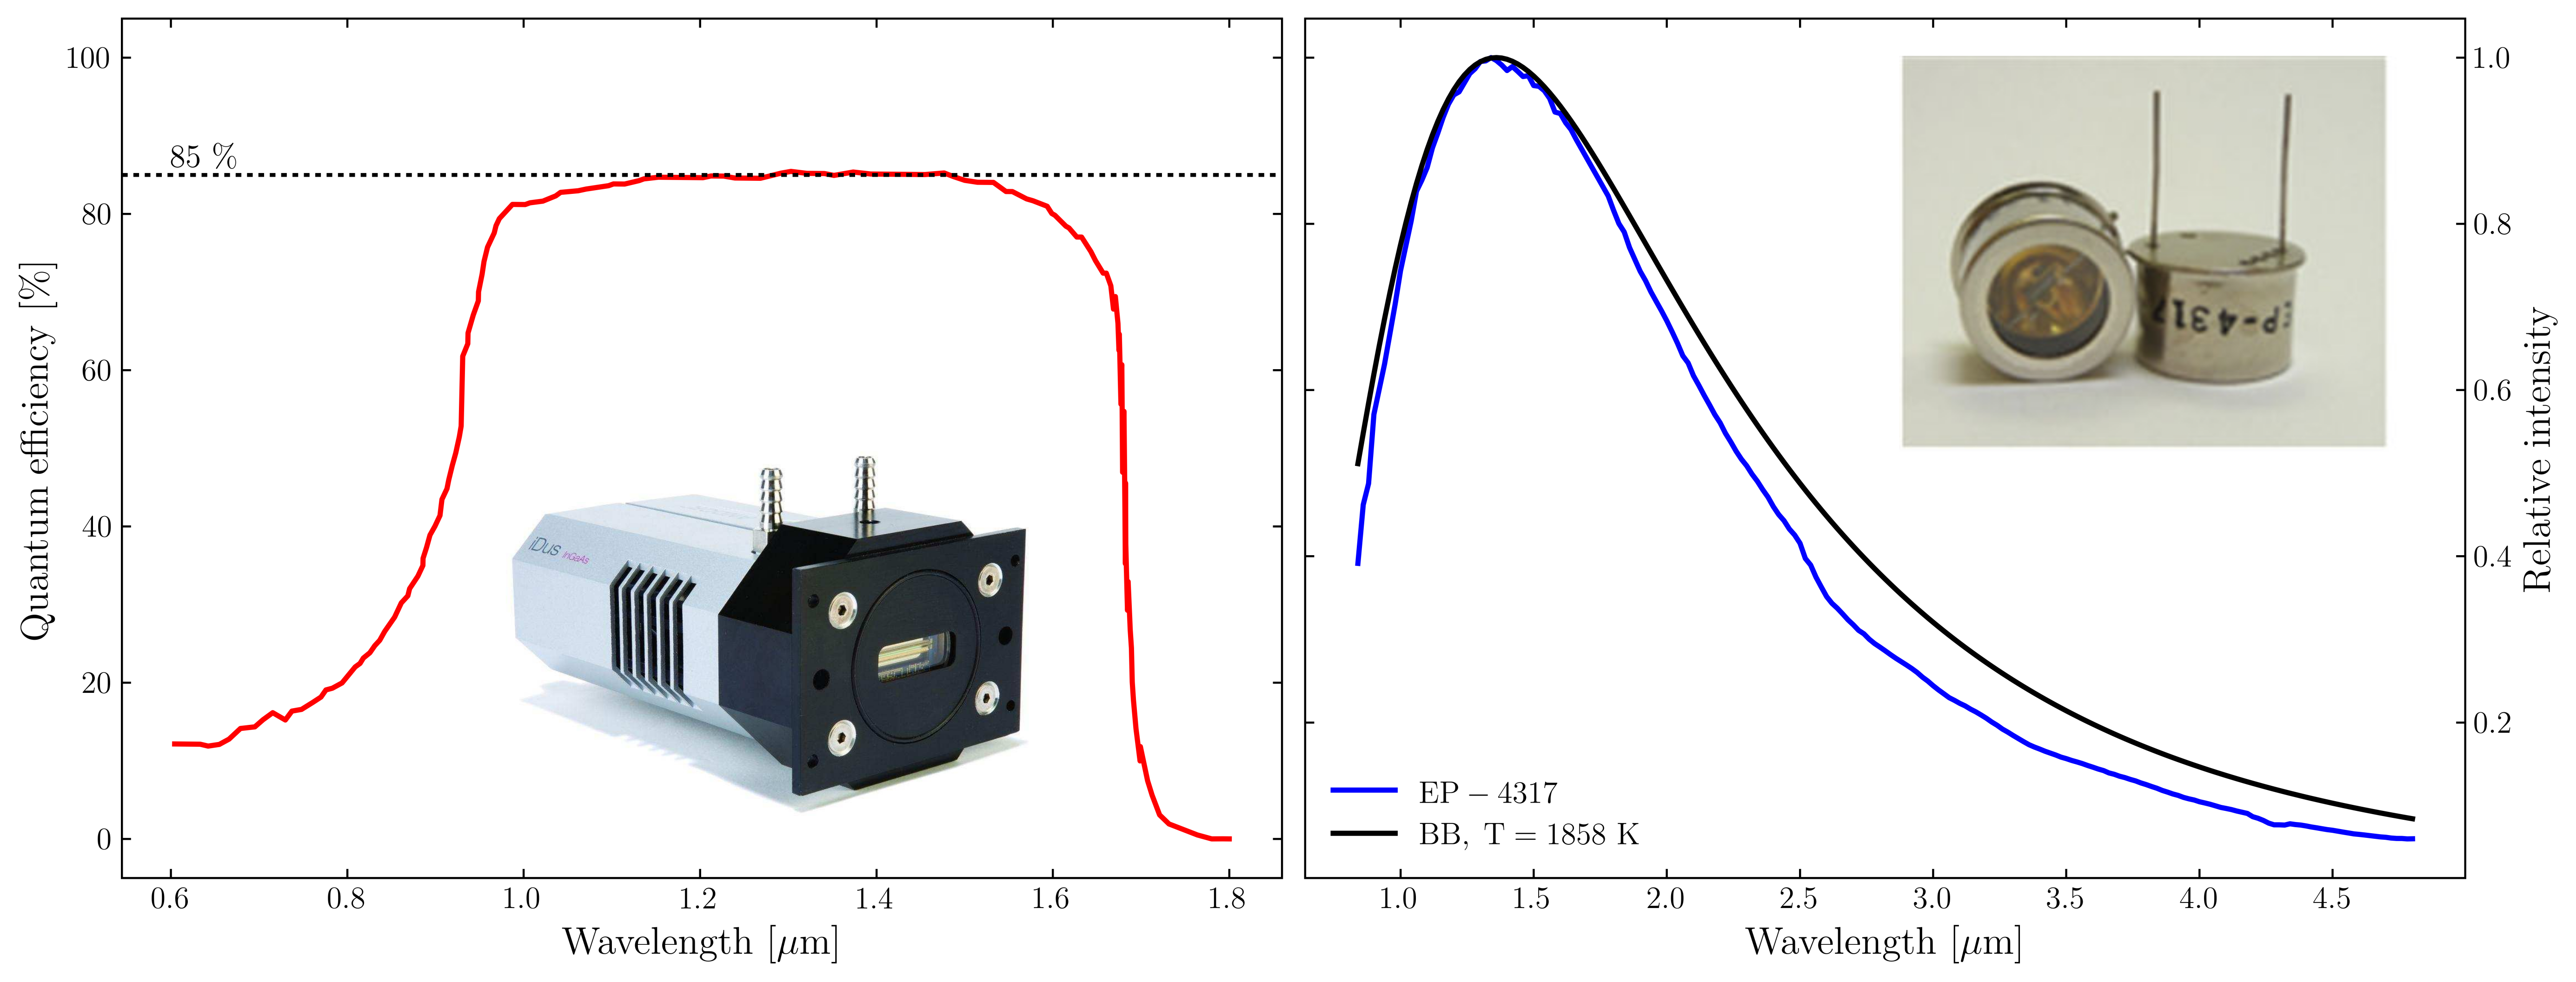
\includegraphics[width=0.9\linewidth]{/Sci_rep/article/ANDOR}
	\caption{Quantum efficiency of used \textit{ANDOR DU490A} camera at $T=20~^\circ$C, taken from Ref.~\citep{manual_andor}, and emission spectrum of a calibration source \textit{EP-4317} from Ref.~\citep{manual_BB} with its emission described by the Planck's law~\citep{Planck_law} characterized by temperature $T=1858~^\circ$C.}
	\label{fig:calib_scirep}
\end{figure}

\section{Photoluminescence measurements}
%
We show our experimental results for one sample with type-II QDs in Fig.~\ref{fig:sci_rep_typeII}. We measured PL spectra for a set of laser pumping powers $P$ and for each of those also the polarization anisotropy defined by a degree of polarization $C(\alpha)$
\begin{equation}
C(\alpha)=\frac{F(\alpha)-F_\mathrm{min}}{F_\mathrm{max}+F_\mathrm{min}},
\end{equation}
where $\alpha$ is the angle corresponding to the crystallographic direction in the plane of the sample, $F_\mathrm{mix}$ and $F_\mathrm{max}$ are extremal values of the oscillator strength of the interband optical transition~$F$. The maximum of the degree of polarization $C_\mathrm{max}$ occurs in a direction given by the angle $\alpha_\mathrm{max}$. The spectra were fitted by a sum of 4~Gaussian functions and appropriate recombination channels were assigned, see Fig.~\ref{fig:sci_rep_typeII}~(a). The assignment was based on (i) the exponent $a$ of $F\propto P^a$, see Fig.~\ref{fig:sci_rep_typeII}~(b), (ii) the azimuth $\alpha_\mathrm{max}$, see the polar graphs at the bottom of Fig.~\ref{fig:sci_rep_typeII}, and (iii) comparison with the theoretical calculations summarized in Sec.~\ref{sec:scirep_theory}. The type of the confinement was determined by the observation of the blue-shift of the normalized PL spectra with increasing $P$ for type-II, or its absence for type-I, see panel~(a).

We clearly identified the recombination of $X^0$ with emission energy of 980~meV, $X^-$ and $XX^0$ in our PL spectra. The measured energy separation of the latter complexes from $X^0$ are $X^- - X^0=76$~meV and $XX^0-2X^0=162$~meV, i.~e. considerably shifted to higher energies as predicted by the theory, see Fig.~\ref{fig:Sci_rep_theory}. As expected, the band $X^+$ cannot be distinguished from $X^0$ in our PL measurements since the energy separation $X^+-X^0$ is much smaller than the inhomogeneous spectral broadening of the emission bands from GaAsSb capped InAs QDs.
%
\begin{figure}
	\centering
	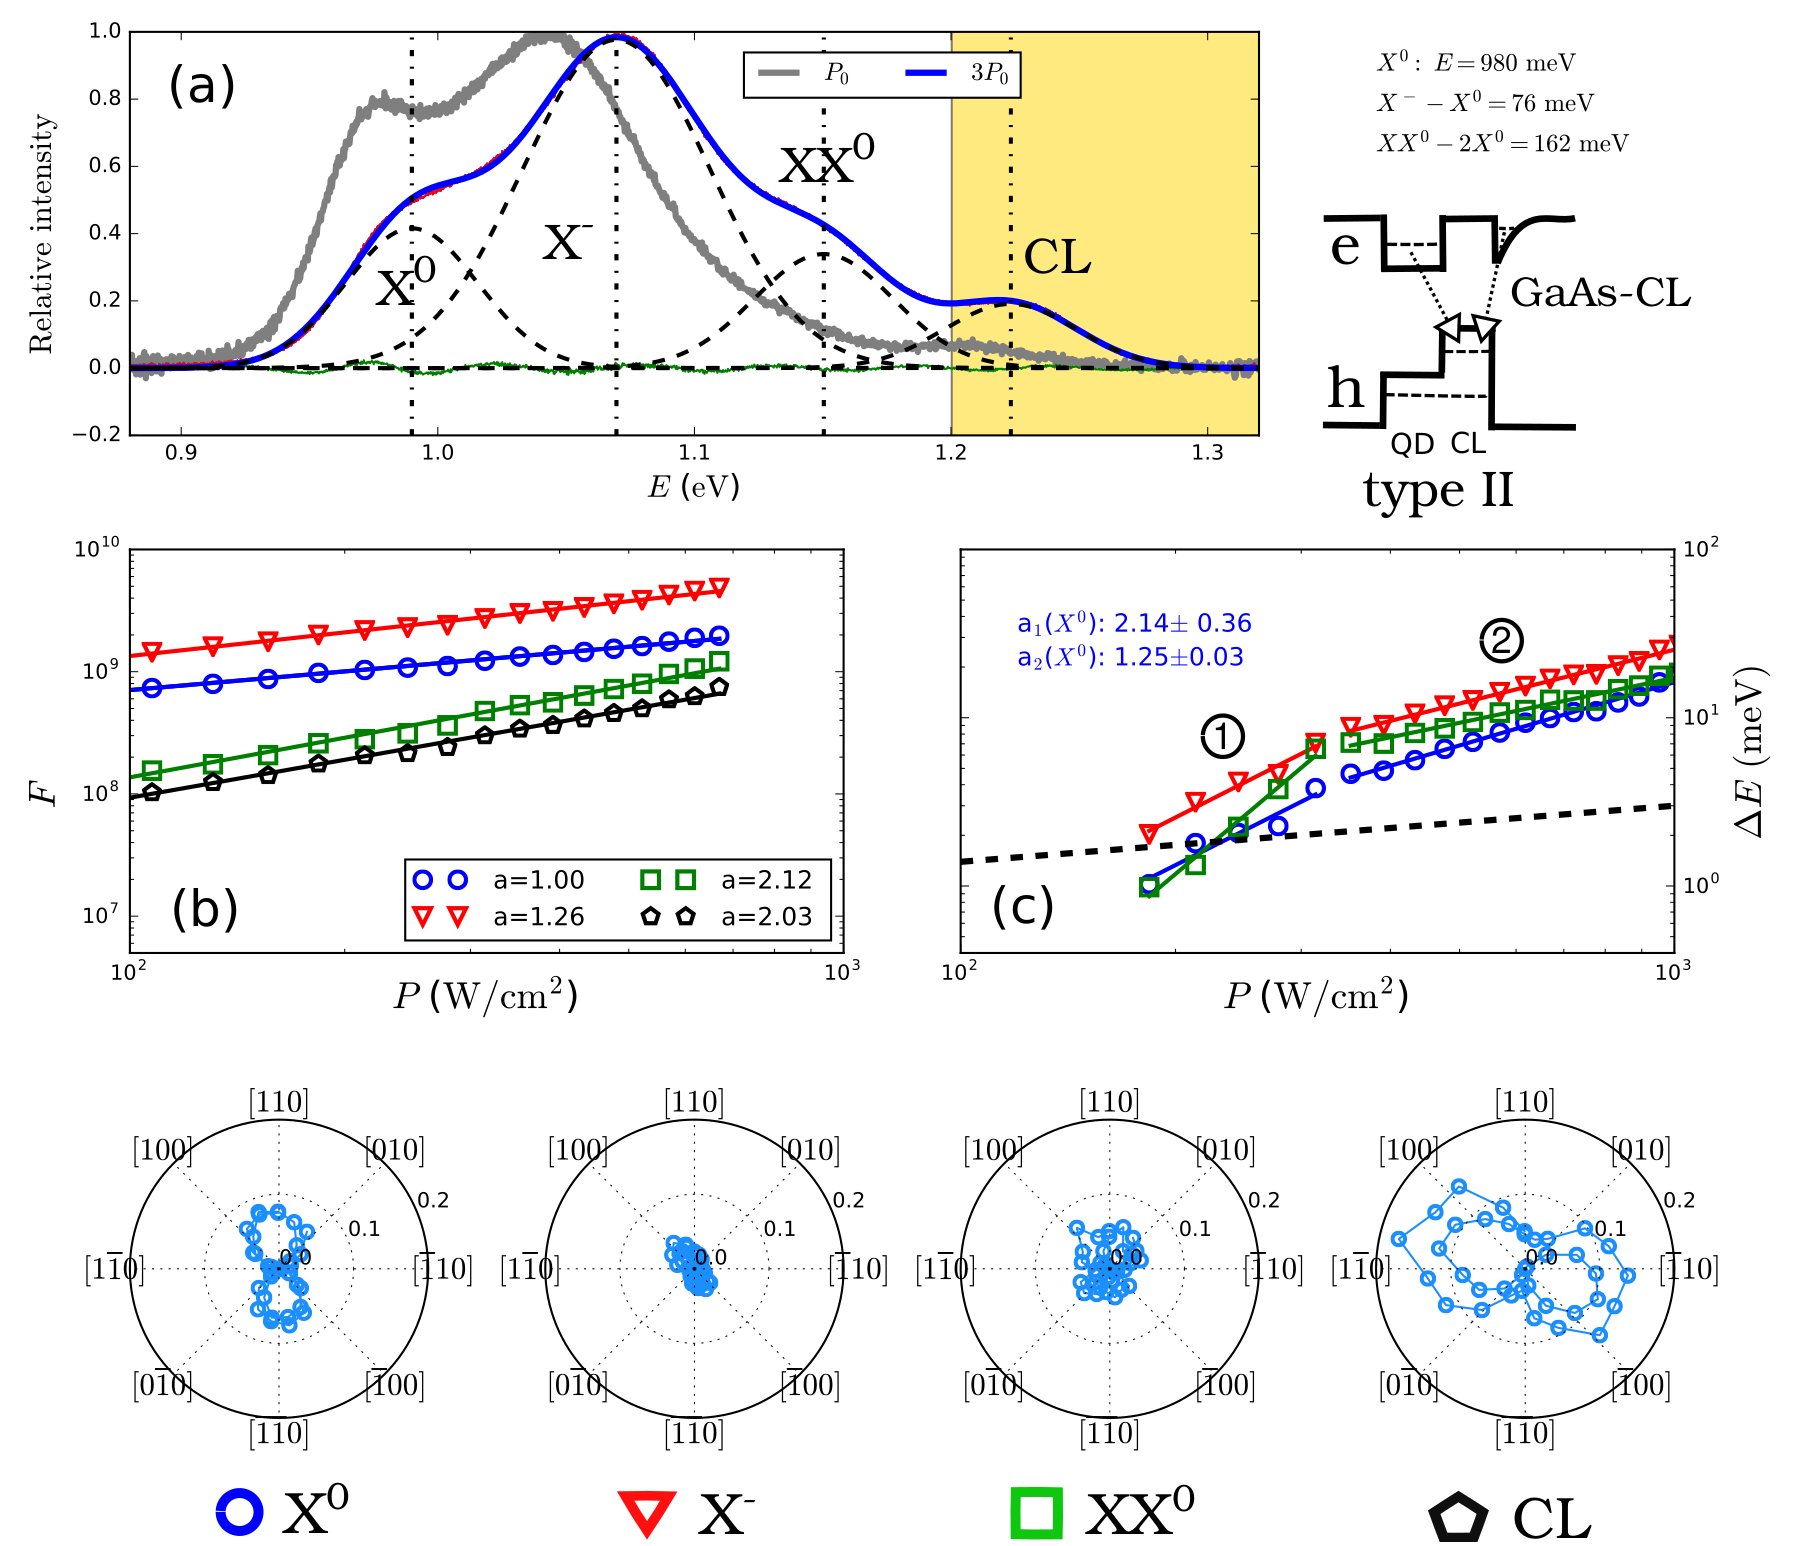
\includegraphics[width=0.9\linewidth]{/Sci_rep/article/type2}
	\caption{(a) PL spectra of GaAsSb capped InAs type-II QDs measured for two pumping powers $P$ (grey for $P_0=1.7$~mW and blue curve for $3P_0=5.1$~mW). The fit by a sum of 4~Gaussian profiles is shown for the PL spectrum obtained under 5.1~mW excitation power and the individual bands corresponding to different multi-excitonic transitions are shown by dashed lines. The difference between measured data and their fits is represented by the green line. The vertical dotted lines indicate the energies of the bands for $3P_0$. The yellow shaded part of the graph corresponds to the recombination between bulk GaAs and CL. The inset near to the panel~(a) gives the spectral position of the complexes from QDs and schematic band diagram of the recombination processes (not in scale). In (b) we show $P$-dependence of the oscillator strength $F$ of the identified bands in log-log scale and their fits by linear lines for $X^0$ (blue circles), $X^-$ (red triangles), $XX^0$ (green squares), and that for the transition between bulk GaAs and CL (black pentagons). The slopes $a$ (i.e. exponents in the linear plots) of the fitted lines are given in the inset of panel (b), for clarity they were normalized so that $a=1$ for $X^0$. Panel (c) depicts the change of the emission energy $\Delta E$ with $P$ in log-log scale. Except for GaAs-CL transition which was omitted, the labels are the same as in (b) and the data were fitted by two linear functions in segments 1 and 2 (see text). The fitted slopes (i.~e. exponents of the dependencies) $a_1$ and $a_2$ for $X^0$ are given in the inset. The $\Delta E\sim P^{1/3}$ dependence of Ref.~\citep{Hatami1998} is shown by the dashed line. The polar graphs at the bottom show $C(\alpha)$ of individually identified bands.}
	\label{fig:sci_rep_typeII}
\end{figure}

The band with the largest emission energy $E$ of 1.21~eV [shaded part of Fig.~\ref{fig:sci_rep_typeII}(a)] is attributed to the recombination between electrons confined due to strain at the interface between bulk GaAs and the GaAsSb CL, and holes within the GaAsSb CL, see also inset Fig.~\ref{fig:sci_rep_typeII}. This transition is purely of type-II nature and exhibits a very large blue-shift with increasing $P$. A~similar recombination pattern has been observed previously for InAsSb QDs~\cite{Mazur2012} and is also responsible for the no-phonon emission from SiGe/Si QDs~\cite{SiGeKlenovsky}. 

To identify the bands also the exponent $a$ of $F\propto P^a$ was used, see log-log scale Fig.~\ref{fig:sci_rep_typeII}~(b). The value of $a$ corresponds to the probability $\mathcal{P}(M)$ that complex $M$ would be excited. The oscillator strength of $X^0$ is, thus, proportional to probability $\mathcal{P}(X^0)$, therefore $F(X^0)\sim \mathcal{P}$. Since the biexciton $XX^0$ can be viewed as a system of two excitons one can expect $\mathcal{P}(XX^0)=\mathcal{P}(X^0)\cdot \mathcal{P}(X^0)\sim \mathcal{P}^2$ behaviour. The trion state $X^-$ (the complex consists of two electrons and one hole) is more probable than $XX^0$ but less than $X^0$ because in order to excite $X^-$ we need to generate $X^0$ and an extra electron, hence we expected $1<a(X^-)<2$. Note, that we have normalized the values of $a$ to that of the lowest band in emission energy which we attribute to $X^0$, hence $a=1.0$ for $X^0$. The other $a$'s are $1.26$ for $X^-$, 2.12 for $XX^0$ and 2.02 for the transition between bulk GaAs and CL, respectively.


In Fig.~\ref{fig:sci_rep_typeII}~(c) in log-log scale the energy shift $\Delta E$ of the PL bands with increasing $P$ defined by
\begin{equation}
\Delta E(P)= E(P) - E(P_\mathrm{min}),
\end{equation}
is shown, where $P_\mathrm{min}$ is the lowest value of $P$ used in the corresponding experiment. In addition to a considerable blue-shift of the bands, which is as large as 30~meV for our values of $P$, it can be seen that (i) $\Delta E$ is different for different $M$ and (ii) there is an edge in the power dependencies meaning that $\Delta E(P)$ 
does not follow the simple form of $\Delta E\sim P^a$ for all values of $P$ but that for each of the two segments 1 and 2 different exponents $a_1=2.14\pm0.36$ and $a_2=1.25\pm0.03$, respectively, seem more appropriate. That effect, observed also elsewhere~\citep{Muller-Kirsch2001}, is significantly different from the $\Delta E\sim P^{1/3}$ dependency predicted in Ref.~\citep{Hatami1998}, which is displayed as a dashed line for comparison.
Moreover, there are differences between the values of the exponents for different complexes. We postpone the explanation of the pumping dependent blue-shift to Sec.~\ref{sec:scirep_pumpingmodel}.

The polar graphs at the bottom of Fig.~\ref{fig:sci_rep_typeII} show that radiation of the recombination of complexes $M$ from the dots is polarized along [110]~crystallographic direction, which means that holes are located in the CL close to the QD base~\citep{Klenovsky2015}. Sharing the same $\alpha_\mathrm{max}$ for all $M$s confirms the prediction that all complexes due of the studied ensemble PL are polarized along the same direction, see Ref.~\citep{Klenovsky2017}. Moreover, the measurement of $\alpha_\mathrm{max}$ allows us to clearly distinguish the GaAs-CL band from the recombinations originating from QD states owing to their perpendicular polarization~\citep{Alonso-Alvarez2011a}.

In Fig.~\ref{fig:scirep_typeIq} we present PL measurements of QDs with type-I confinement in the same manner as in Fig.~\ref{fig:sci_rep_typeII}. We again identify $X^0$, $X^-$, $XX^0$ and the GaAs-CL transition, respectively, with the similar positions of $M$s to type-II QDs. Exciton $X^0$ is positioned at 982~meV, and $X^-$ and $XX^0$ are shifted to higher energies of about 80~meV and 173~meV, respectively. Similarly, considerable increase of $X^--X^0$ and $XX^0-2X^0$ occurs due to the fact that even a rather small increase in CL thickness results in a large increase of binding energies, as can be seen in Fig.~\ref{fig:Sci_rep_theory}. 
%
\begin{figure}
	\centering
	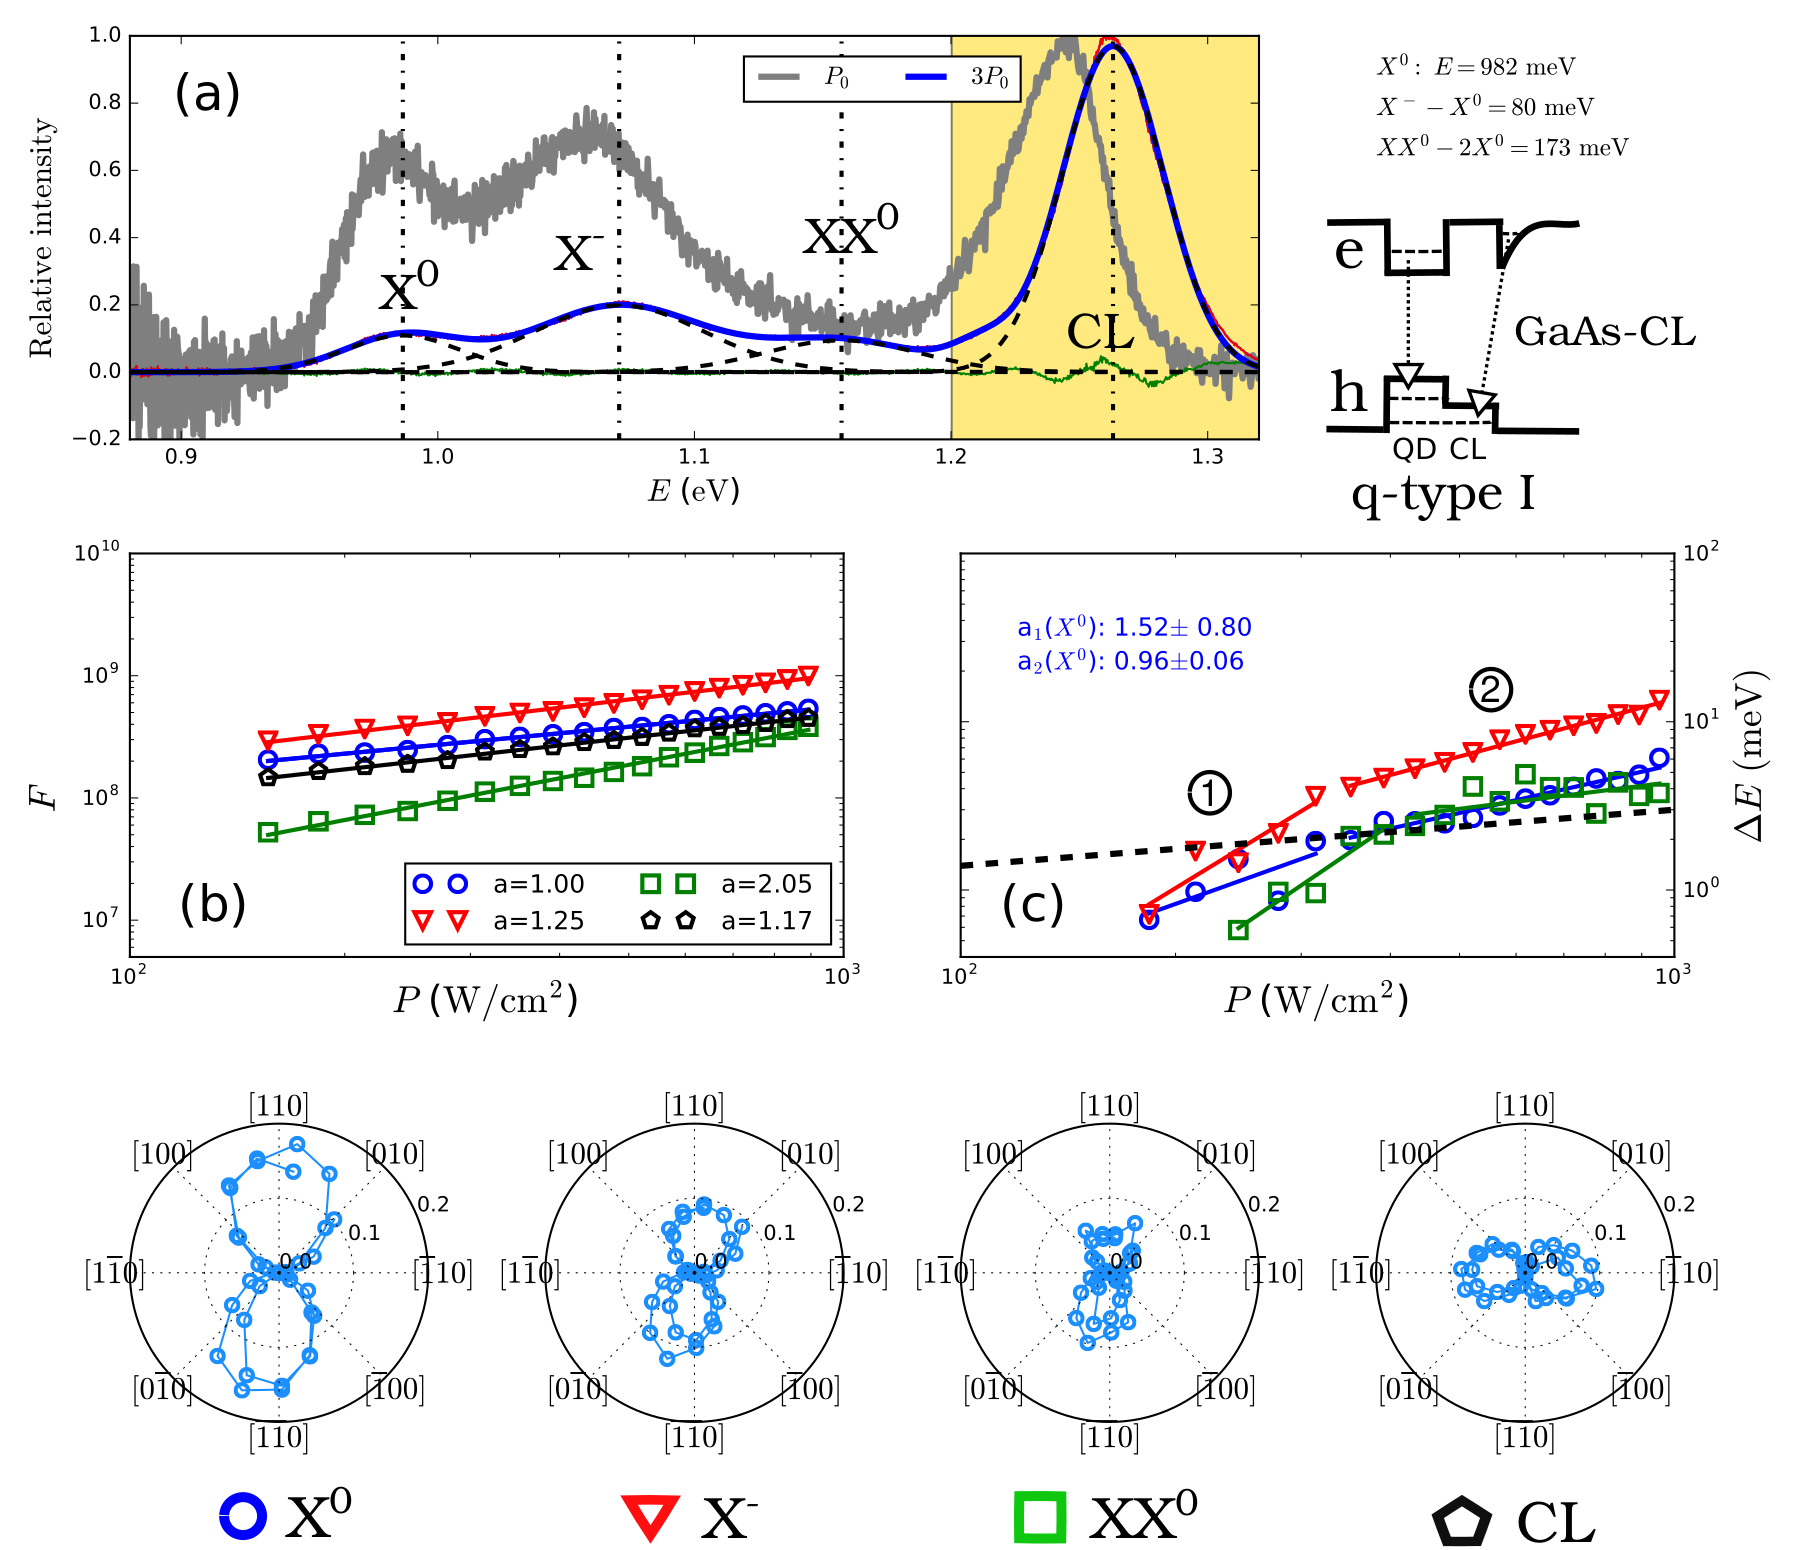
\includegraphics[width=0.9\linewidth]{/Sci_rep/article/typeI}
	\caption{PL spectra of GaAsSb capped InAs q-type-I QDs. The results are similarly commented as in Fig.~\ref{fig:sci_rep_typeII}.}
	\label{fig:scirep_typeIq}
\end{figure}
%
In fact, the type of confinement is not purely of type-I in GaAsSb capped InAs QDs for Sb contents different from zero, since even a slight increase of that lowers the confinement for holes in CL with respect to GaAs~\cite{Klenovsky10}, see inset of Fig.~\ref{fig:scirep_typeIq}. Thus, the excited single-particle states tend to be partly localized in the CL which results in a slight blue-shift of $X^0$ with increasing $P$ and also $a_1=1.52\pm0.80$ and $a_2=0.96\pm0.06$ are not equal to zero, see Fig.~\ref{fig:scirep_typeIq}~(c). We call this type of confinement \enquote{quasi-type-I} (q-type-I). For results of the true type-I confinement represented by InAs/GaAs QDs for which no blue-shift of $X^0$ with $P$ is observed and $a\approx0$, see Fig.~\ref{fig:671C}. We note that slightly larger values of $X^--X^0$ and $XX^0-2X^0$ for type-II and q-type-I in Figs.~\ref{fig:sci_rep_typeII} and~\ref{fig:scirep_typeIq}, respectively, compared to Fig.~\ref{fig:Sci_rep_theory} are probably due to the spatial inhomogeneity of the In distribution in the QDs, and of Sb in the CL, which were not considered in our theory. 

The polarization anisotropy of q-type-I QDs is again oriented along [110], see the bottom of Fig.~\ref{fig:scirep_typeIq}, and its degree is larger than for type-II in agreement with the trend for very thin CL discussed in Ref.~\citep{Klenovsky2017}. The GaAs-CL transition is again perpendicularly polarized compared to the emission of QD bands. Since the confinement for holes in the CL is larger for type I than for type II, the emission energy of GaAs-CL band is larger in type I. The energy of the GaAs-CL band also blue-shifts with pumping by a much larger amount than for the q-type-I QD bands and, thus, this structure represents a coexistence of type-I and type-II confinement~\cite{Ji2015}.


The pumping power dependence of PL from type-I InAs/GaAs QDs is shown in Fig.~\ref{fig:671C}. Using oscillator strength dependencies on $P$ we identify  $X^0$ and $XX^0$ optical transitions with appropriate slopes $a=1$ and $a=2.13$, respectively, with emission anisotropy along [110] crystallographic direction observed previously in, e.~g.,~\citep{HumPhysE}. Note particularly, that the energy of $X^0$ does not change with $P$, i.~e. $\Delta E\approx 0$. On the other hand, large blue-shift of $XX^0$ with $P$ is due to the structure of the sample. It is a stack of 3 layers of InAs QDs grown above each other. Due to that $XX^0$ in Fig.~\ref{fig:671C} originates in transitions when the quasi-particles are located in different QDs of the multilayer and are thus of type-II displaying considerable blue-shift with $P$. We note that biexcitons originating in transitions from one QD cannot be resolved by our PL measurements.
%
\begin{figure}
	\centering
	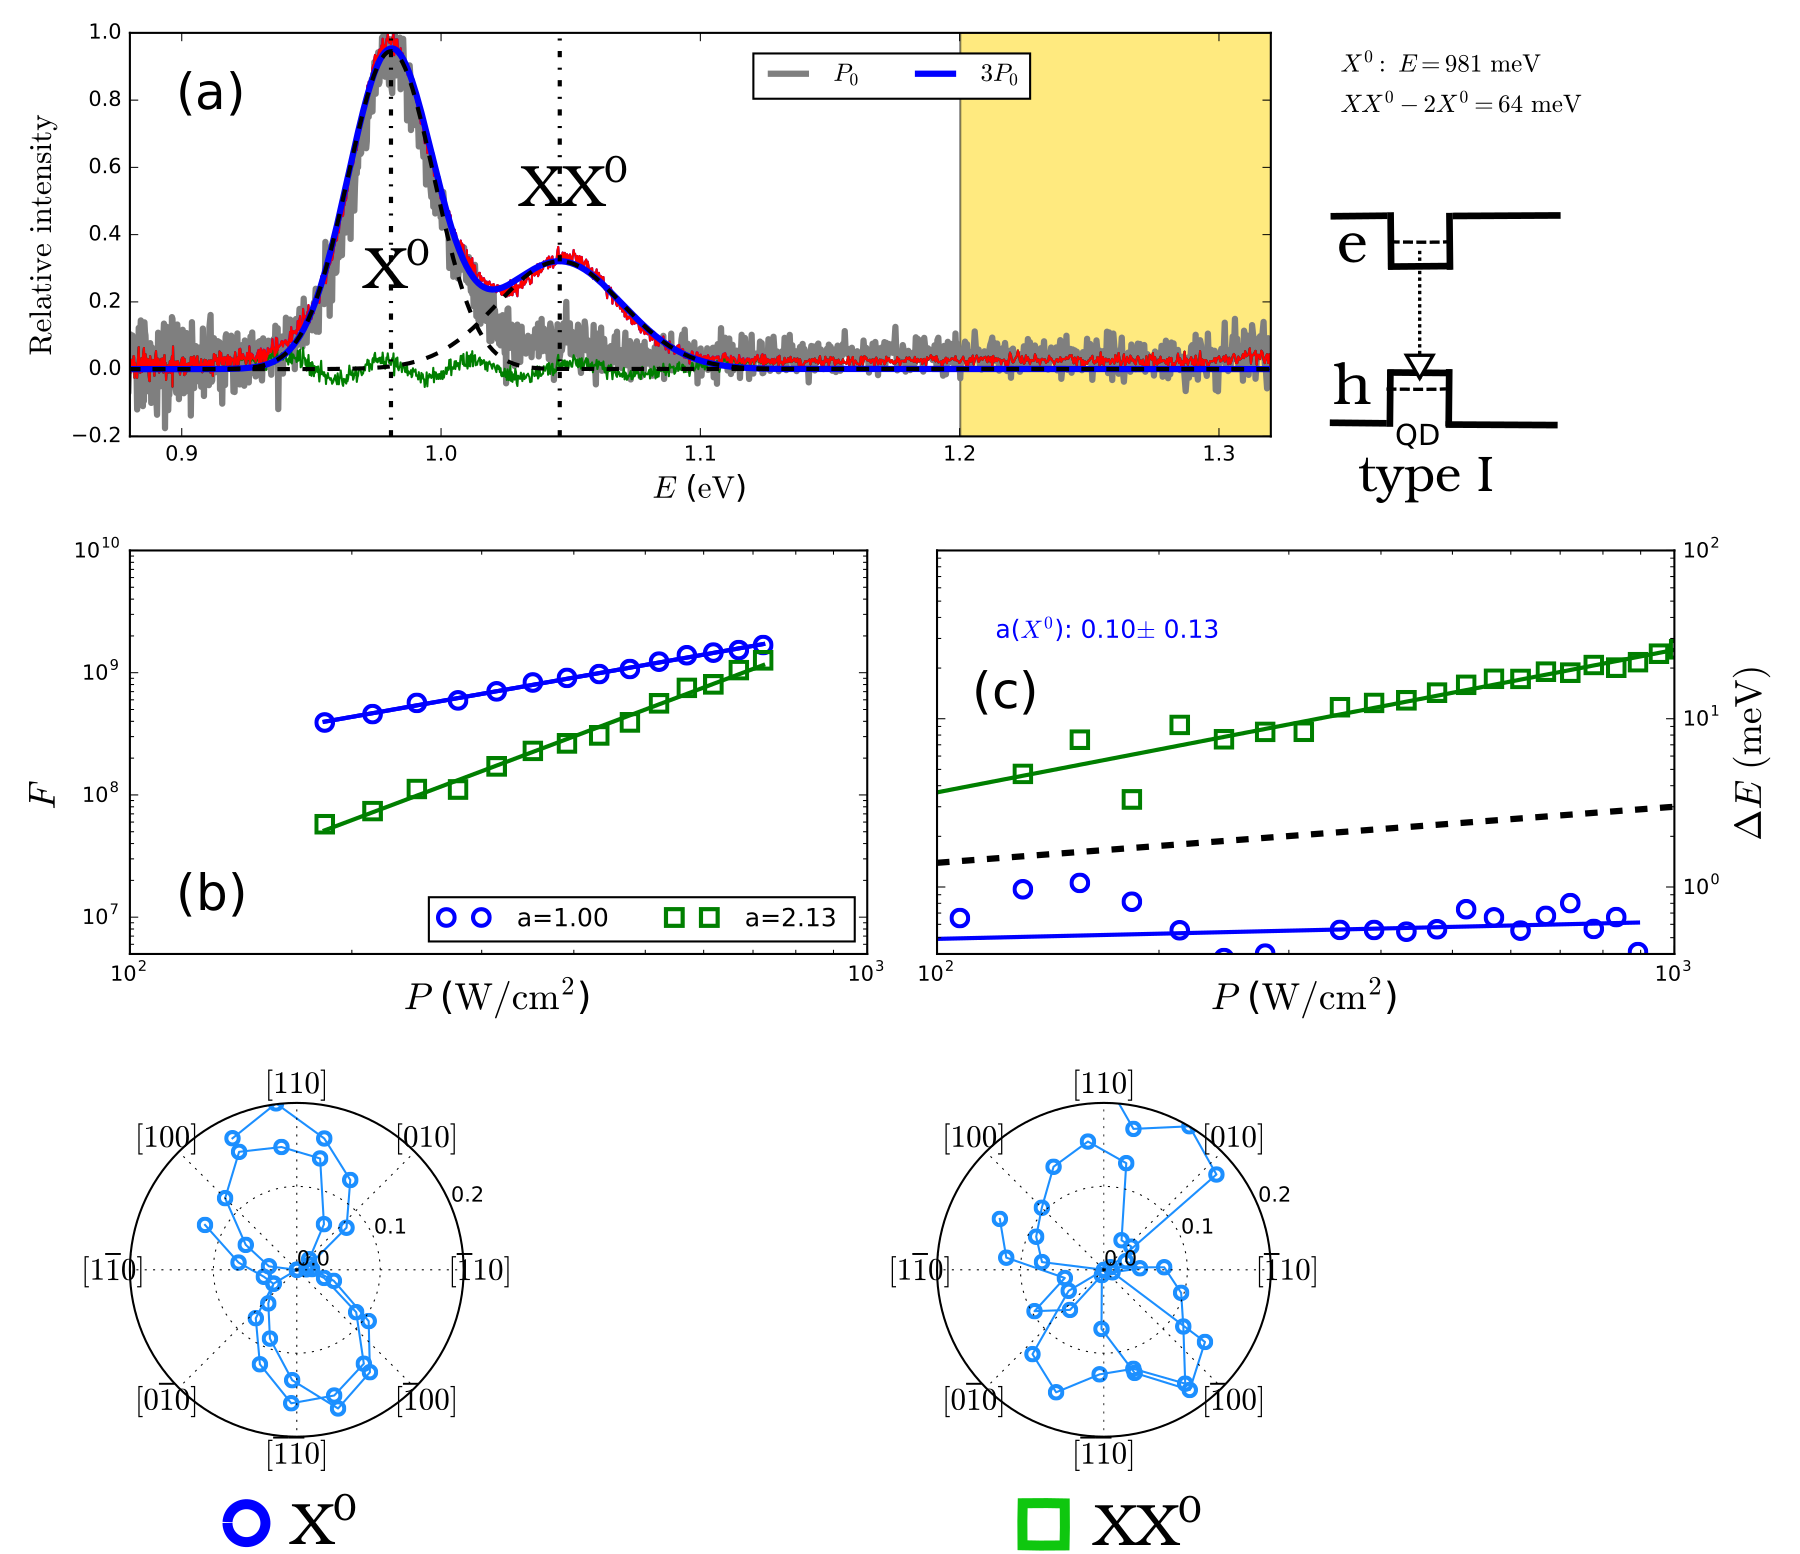
\includegraphics[width=0.9\linewidth]{/Sci_rep/article/671C}
	\caption{Results for type-I InAs/GaAs QDs. The outline of the figure is similar as in Fig.~\ref{fig:sci_rep_typeII}.}
	\label{fig:671C}
\end{figure}

In order to make our results more general we repeated the aforementioned measurements on 16~different QD samples. The results of those are given in the Appendix~\ref{chapter:appendix_SciRep} in Figs.~\ref{fig:sup:osc_slope} for the exponent in $F\propto P^a$, Fig.~\ref{fig:sup:mean_blueshift} for the mean emission energy shift, Fig.~\ref{fig:sup:mean_a_blueshift} for the mean $a$ in $\Delta E \propto P^a$, and Fig.~\ref{fig:sup:pol} for $\alpha_{\mathrm{max}}$, and $C_{\mathrm{max}}$, respectively.
\newpage 





\section{Model of blue-shift}\label{sec:scirep_pumpingmodel}
In PL experiments the blue-shift of the emission energy $\Delta E$ with increasing $P$ in type-II confined QDs is usually observed, however, the physical nature of this phenomenon is still discussed. Currently, two competing hypotheses are put forward in this respect.

The \textbf{state-filling} model stemming from the observation of large radiative lifetime of the emission from type-II QDs~\citep{Liao2009,Nishikawa2012,Sato2012,Pavarelli2012,Young2014}. In this model, the blue-shift is caused by a larger proportion of the radiative transitions between electronic levels higher in energy than the ground state if the pumping rate exceeds the emission rate of the ground state transition which is often the case for type-II QDs~\citep{Gradkowski2012}. In addition to this energetic aspect, the spatial localization of the wave functions associated with the states involved in the state-filling induces a capacitive charging effect~\citep{Muller-Kirsch2001}, also contributing to the overall blue-shift of the emission.


The second hypothesis dubbed \textbf{band-bending} explains blue-shift as a change of the confinement potential for holes close to QD~\citep{LiuSteer,Jin,Hatami1998,Jo2012}. In the specific framework of infinite triangular quantum wells, it was speculated that this mechanism induces a $\Delta E \propto P^{1/3}$ dependence~\cite{Ledentsov1995,Kuokstis2002,Jo2012}. While the validity of this power law for different systems is arguable, it was often used in the literature for discussing the properties of GaSb/GaAs QDs~\cite{HATAMI1995,Hatami1998}.

Our experimental results presented in Figs.~\ref{fig:sci_rep_typeII} and \ref{fig:scirep_typeIq} are not consistent with the power law usually associated with band-bending, and require a specific interpretation. Therefore, we follow an approach similar to that of Gradkowski{~et~al}., see Ref.~\citep{Gradkowski2012}. Because electronic states in QDs are multi-particle in nature, we employed so-called semi-self-consistent CI (SSCCI) approach developed by the supervisor to characterize the energy shift with $P$.

We now proceed with overview of SSCCI method. Firstly, a certain concentration of background electrons $c_\mathrm{e}$ in QD body and holes $c_\mathrm{h}$ in CL were defined, reflecting the spatially indirect nature of charges in the type-II system, to produce a background electric potential in QD and CL. Because we investigate system in a steady-state pumping regime, $c_\mathrm{h}-c_\mathrm{e}=0$. In other parts of the simulation space (GaAs matrix) we set $c_\mathrm{h}=c_\mathrm{e}=0$. Then, the single particle Schrödinger and Poisson equations for the system with these background potentials are solved self-consistently with all diagonal matrix elements of $J_\mathrm{eh}$ resulting from the CI calculation set to zero since we assume those to be already included in the single-particle energies obtained from the preceding self-consistent cycle.

The correspondence of concentration used in simulations with experimental values of $P$ is obtained by~\cite{Kuokstis2002}
%
\begin{equation}
\label{eq:conc_to_P_recalc}
P=\frac{10^6\gamma E_{l}}{\alpha}c_\mathrm{q}^2,
\end{equation}
where $c_\mathrm{q}=c_\mathrm{e}=c_\mathrm{h}$ is the number of electron-hole pairs generated by a laser light with the emission energy $E_l$ (in our case 1.58~eV), $\alpha$ is the absorption coefficient of the sample material ($2.0\times 10^4$~cm$^{-1}$ for GaAs~\cite{landoltbornstein}), and $\gamma$ is the radiative recombination coefficient ($7.0\times 10^{-10}$~cm$^3$s$^{-1}$ in the case of GaAs~\cite{landoltbornstein}).

The results of the blue-shift of multi-excitonic energies with $P$ calculated by SSCCI are presented in Fig.~\ref{fig:scirep_pumpmodel} for CL thicknesses of 3~and~8~nm. Our model correctly predicts the \enquote{bending} of $\Delta E$ in panels~(c) of Figs.~\ref{fig:sci_rep_typeII} and \ref{fig:scirep_typeIq}, and the presence of different slopes in the log-log graphs [indicated by marks 1 and 2 in Fig.~\ref{fig:scirep_pumpmodel}~(a)].  The fitted exponents (slopes in log-log graphs) are $a_1=0.87\pm0.02$ and $a_2=0.07\pm0.02$ for $d=$3~nm, and $a_1=0.54\pm0.02$ for 8~nm, respectively. For type II the exponent in sector 1 decreases while that in sector 2 increases with increasing $d$, up to an approximate $\Delta E\sim P^{1/3}$ dependence reached for thick CLs. The blue-shift is accompanied by a change of the spatial distribution of the hole wavefunction~\cite{Gradkowski2012}, see insets of Fig.~\ref{fig:scirep_pumpmodel}~(b): holes are \enquote{squeezed} towards the QD body and, thus, towards the electrons~\cite{Gradkowski2012,Llorens2015}. 
%
\begin{figure}
	\centering
	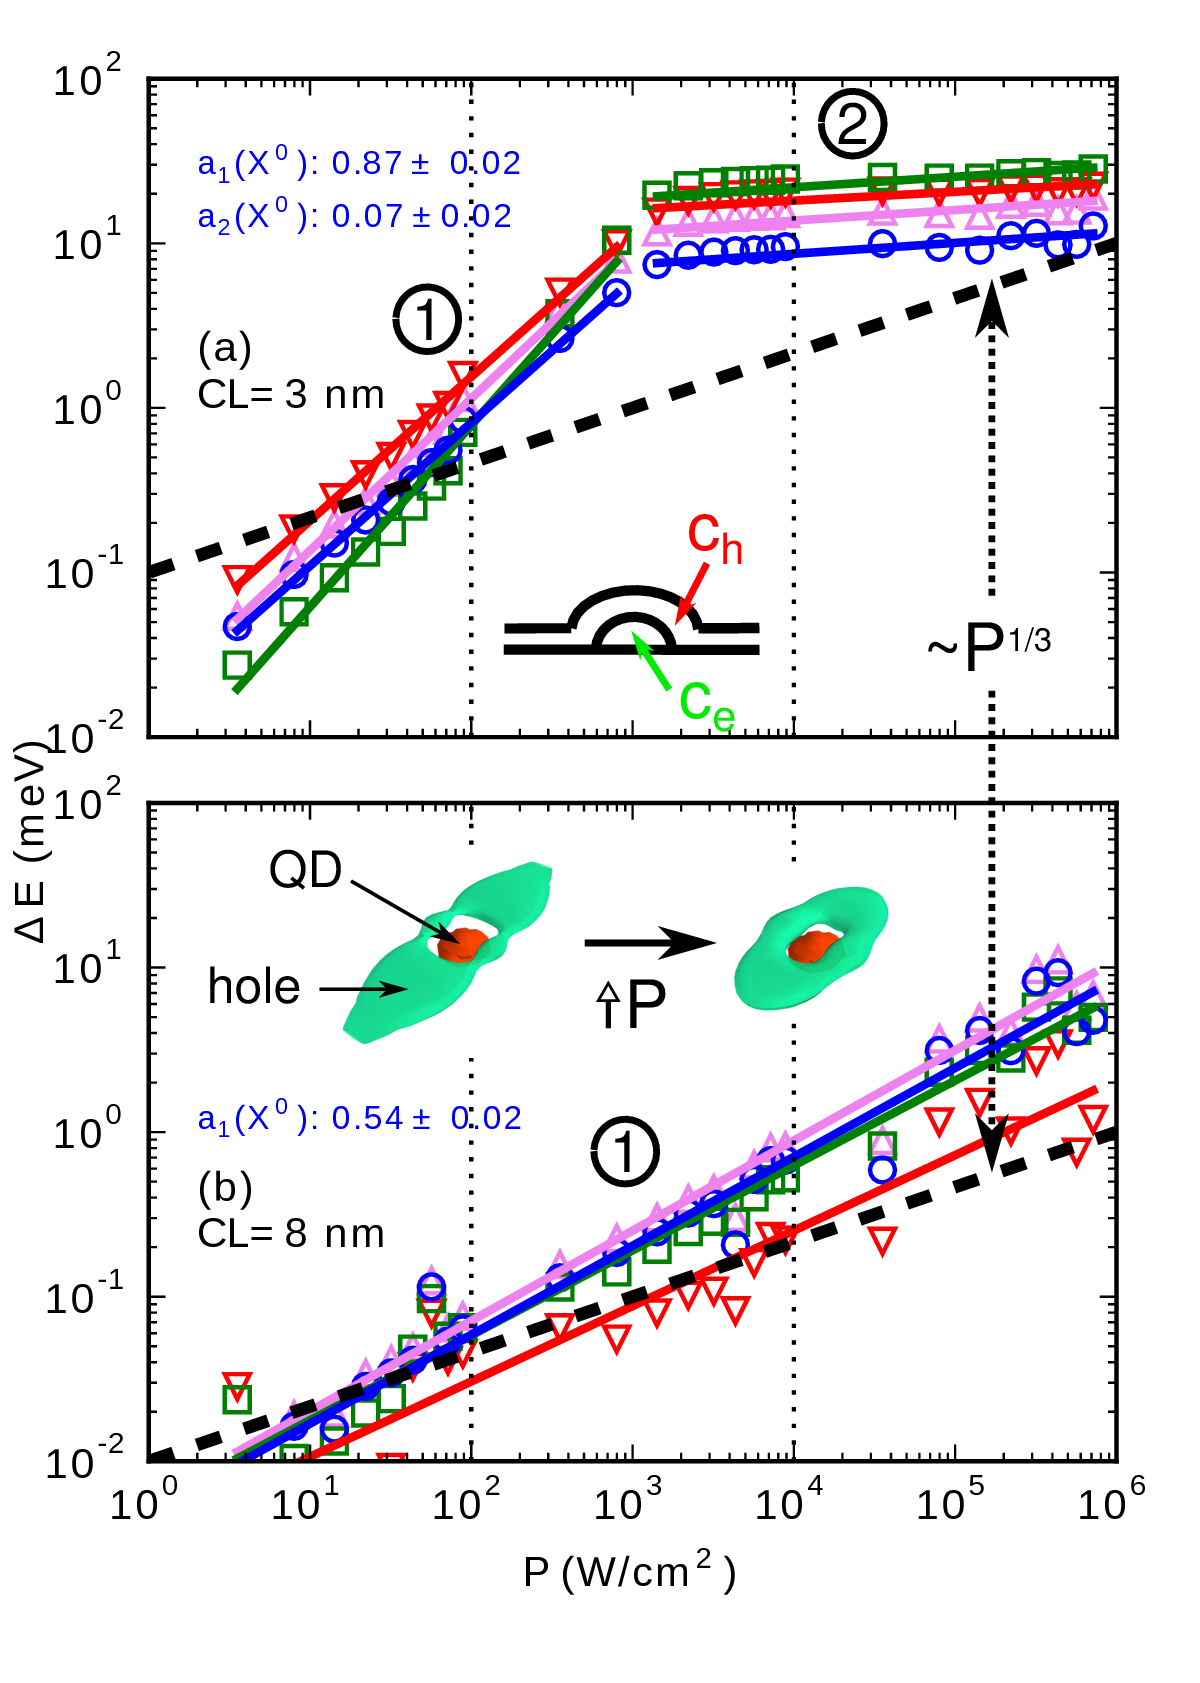
\includegraphics[width=0.68\linewidth]{/Sci_rep/article/pump_model}
	\caption{Energy shift $\Delta E$ as a function of $P$ for CL thickness $d$ of (a) 3~nm and (b) 8~nm for $X^0$ (blue circles), $X^+$ (magenta upward triangles), $X^-$ (red downward triangles), and $XX^0$ (green squares). The inset in (a) shows the background electron ($c_\mathrm{e}$) concentration in QD and hole ($c_\mathrm{h}$) in CL. The inset in (b) gives the hole probability density of 50~\% (green isosurfaces) for $d=8$~nm and two values of $P$; the dot is marked as a red lens in the middle of the hole wavefunction. The numbers 1 and 2 mark different segments of the dependency similarly to Figs.~\ref{fig:sci_rep_typeII} and \ref{fig:scirep_typeIq}. The fitted exponents $a_1$ and $a_2$ of $X^0$ are given in the insets of both panels. The dotted vertical lines in both panels roughly border the intervals where we have obtained in the measurements in Figs.~\ref{fig:sci_rep_typeII}  and~\ref{fig:scirep_typeIq}.}
	\label{fig:scirep_pumpmodel}
\end{figure}

The difference in $a_1$ between thinner and thicker CL can be qualitatively understood by inspecting the change in the lateral electron-hole dipole moment $p_{xy}$ with $P$. The total lateral potential for holes in type-II QDs might be written as $V_{xy}^\mathrm{total}=V_{xy}^\mathrm{bulk}-V^{\mathrm{piez}}_{xy}$, where $V^{\mathrm{bulk}}_{xy}$ is the energy of the holes in the bulk semiconductor. With increasing $P$ the hole wavefunction is shifted towards that of the electrons, thus $V^{\mathrm{piez}}_{xy}$ is reduced, so that both $V^{\mathrm{total}}_{xy}$ and the single-particle transition energies increase. Because $p_{xy}$ is larger in the QDs with thin CL than in those with a thick CL, we can infer that the rate of blue-shift of single-particle transition energies with $P$ should be larger for QDs with thinner CLs.

The meaning of $c_\mathrm{e}$ and $c_\mathrm{h}$ in our calculations is that of an average occupation of charge traps~\cite{Reimer2016} in QD and CL, respectively, thus, there is probably an important contribution of trap-state filing effect. 

Finally, our model of blue-shift is more consistent with the \enquote{band-bending} hypothesis presented above if the changes of the confinement potential of quasiparticles are due to filling of charge traps.

\section*{Conclusions}
We have experimentally studied the excitonic structure of type-II InAs/GaAsSb/GaAs quantum dots by intensity and polarization resolved photoluminescence spectroscopy. Based on intensity resolved photoluminescence we identify multiparticle optical transitions of neutral exciton, biexciton, and negative trion, respectively. Our identification is supported by full configuration interaction calculations where the similar binding energies of these complexes have been predicted. 

The polarization-resolved photoluminescence allows us to distinguish optical transitions originating from quantum dots, where emission anisotropy of the complexes is oriented along [110]~crystallographic direction, and the transition between bulk GaAs-GaAsSb capping layer interface states and quantum dots having perpendicular orientation of polarization.

The blue-shift of emission energy with increasing excitation laser power is observed for InAs/GaAsSb/GaAs quantum dot samples. This blue-shift is simulated by semi-self-consistent configuration interaction method with added background potential in quantum dot area.

The blue-shift model for thicker capping layer gives similar behaviour as usually used $\Delta E\propto P^{1/3}$ approximation, for thick capping layer, a stronger blue-shift is predicted up to a~critical excitation power followed by slighter increase for thin layer. Finally, this two segment behaviour is also observed experimentally.
\newpage
%https://books.google.cz/books?id=DiFMPmXSsLUC&pg=SA6-PA15&lpg=SA6-PA15&dq=Varshni+1967&source=bl&ots=hBJXnBqrHH&sig=WuCbtLj6FUIWMr09BP1LkBR-2cc&hl=cs&sa=X&ved=0ahUKEwi5mPz5lL_ZAhUGEVAKHRiaAOIQ6AEIXDAH#v=onepage&q=Varshni%201967&f=false

\chapter{InGaAsSb/GaAs/GaP QDs for Flash memories}\label{chap:TUB_QD}

%The direct-band gap semiconductor InGaAs represents the basic of the active area of a multitude of commercial photonic devices
%Optical emitters are one of the key components of optoelectronics and photonics. Despite the considerable progress in light emitting technology in visible spectral range during the last decades, the implementation of efficient light emitters on silicon remains a challenge. 
Today's market of computer memories is divided mainly between two kinds of memories, i.~e., the dynamical random access memory (DRAM)~\citep{waser_2003} and the flash memory~\citep{Pavan_1997}. The DRAM is fast but volatile, which means that the information must be refreshed within every tens milliseconds. On the other hand flash memory is a non-volatile memory with a storage time of more than ten years without any power consumption, however, it suffers from a slow write time of several microseconds. Semiconductor memory community is seeking for a memory based on the advantages of both previous types, which would combine the fast write/read speed with long storage time. Different approaches toward that goal are studied at the moment, such as FeRAM, MRAM or PCRAM, etc.~\citep{Burr_IBM2008}.

One of the promising options to combine fast write speed and long storage time is the use of QD-Flash~\citep{Geller_APL2008_QDFlash}, a memory based on self-organized quantum dots (QDs) fabricated from III-V materials. These nano-objects can be prepared by Stranski-Krastanov growth mode and due to a variety of material band structure engineering its band-offsets and barriers can be tuned in contrast to the fixed SiO$_2$ barriers in the current Flash memories.\\
%
\indent Storage of information is always a non-equilibrium situation, which is lost after a certain time. In the QD-based memory this process is limited by certain time of thermal emission only. The storage time for various materials based on either electron~\citep{Anand_apl1995_elflash,Nowozin_2013_sum} or hole~\citep{GellerPRB, stracke_apl2012_qdflash_GaP,Nowozin_2013_sum} storages were studied. The energy levels of confined holes in a QD are much more favourably confined than those of electrons owing to their larger effective mass, therefore, at least one order of magnitude more holes can be stored in a given volume than electrons. \\
%
\indent One of the suitable systems for realization of long storage time QD-Flash are heterostructures grown on GaP substrate. For In$_{0.25}$Ga$_{0.75}$As/GaAs/GaP the storage time of 3~$\mu$s was measured at room temperature~\citep{stracke_apl2012_qdflash_GaP}, which is insufficient for memory usage, however, it is already three orders higher than the time for a typical representative of III-V QDs from InGa/GaAs~\citep{GellerPRB}. Longer storage time can be expected in the GaSb/GaP system, due to higher localization energy. Several pioneering studies have been reported for GaSb/GaP system, where the storage time is predicted in a range 1 and $10^5$ years with 8-band $\mathbf{k\cdot p}$ calculations~\citep{Bimberg_proceedingSPIE}, however the experimentally observed times were not larger than 3.9~days~\citep{Bonato_pssolidi_GaSbonGaP}.\\%  Moreover, the storage time for GaSb/GaP heterostructure was predicted in a range 1 and $10^5$ years with 8-band $\mathbf{k\cdot p}$ calculations~\citep{Bimberg_proceedingSPIE}.\\
%
\indent The use of structures grown on GaP substrate has another benefit besides other III-V semiconductors, where crystalline defects are generated during the III-V/Si heteroepitaxy. It was proposed to use pseudomorphic GaP/Si substrate benefiting from the low lattice mismatch between GaP and Si (0.37~\% at 300~K) to avert the formation of these defects~\citep{Beyer_jap2013,Grassman_apl2013, Lin_jcg2013}. Hence, the GaP-based heterostructures can be implemented in defect-free quality on Si chips.

In this chapter, we follow several previous experimental works which investigated {(In,Ga)As/GaP} QDs. InAs/GaP QDs have first been reported in Refs.~\citep{Leon_apl1998, guo_solidi2009}, but efficient PL was not achieved because of the plastic relaxation due to the large lattice mismatch (11.2\%). Then Futchi et al.~\citep{Fuchi_physicaE2004} measured PL up to 77~K on InGaAs/GaP QDs and pointed to the issue of In composition and dominant role of In amount was demonstrated via calculations~\citep{Fukami_solodi2011}. Rivoire et al.~\citep{Rivoire_prb2012} claimed a single dot emission of type-I In$_{0.5}$Ga$_{0.5}$As/GaP QDs, subsequently, the structural and emission properties were studied~\cite{Stracke_apl2014, Sala_apl2016}. To initiate the Stranski-Krastanov growth mode of In$_x$Ga$_{1-x}$As QDs on GaP, the GaP surfaces need to be covered by thin layer of GaAs prior to In$_x$Ga$_{1-x}$As deposition~\citep{stracke_apl2012_qdflash_GaP}.
%
%
% konec korekci PK
%
%
We investigate a set of samples with In$_{1-x}$Ga$_{x}$As$_y$Sb$_{1-y}$/GaAs/GaP QDs with GaAs thickness of 5~ML by centered around the energy of 1.8~eV, where emission from QDs is expected. We study PL of these samples as function of excitation power and temperature. The dynamics of optical transitions in the studied ensemble is examined by time-resolved PL (TRPL).


\section{In$_{1-x}$Ga$_{x}$As$_y$Sb$_{1-y}$/GaAs/GaP QDs samples}
The samples were grown on GaP(001) substrate by metalorganic vapor phase epitaxy (MOVPE) in Stranski-Krastanov mode in a horizontal Aixton 200 reactor using H$_2$ as carrier gas at Technische Universität Berlin~\citep{Sala_apl2016}. \\
%
\indent The growth starts with 250~nm GaP buffer layer followed by 20~nm AlGaP barrier and 150~nm GaP at the temperature of 750~$^\circ$C. Subsequently the temperature is reduced to 500~$^\circ$C for the following steps: (i) growth of a thin GaAs interlayer (5~ML) for all studied samples, (ii) for samples which we call S$_\mathrm{with}$ and S$_\mathrm{cap}$ a short Sb-flush is applied by supplying the triethyl-antimony for two and one second, respectively, at input flux of $2.6~\mu\mathrm{mol/min}$, (iii) In$_{1-x}$Ga$_{x}$As$_y$Sb$_{1-y}$ QDs growth, (iv) GaSb cap in case of sample S$_\mathrm{cap}$ (v) growth interruptions (GRI) for 1~s, and finishing the structure by GaP capping layer of 6~nm thickness. Finally, samples are heated to 620~$^\circ$C to grow 50~nm thick GaP layer. The samples are depicted in Fig.~\ref{fig:TUstructure} and their differences and labels are summarized in Tab.~\ref{tab:samples}.
\begin{figure}
	\centering
	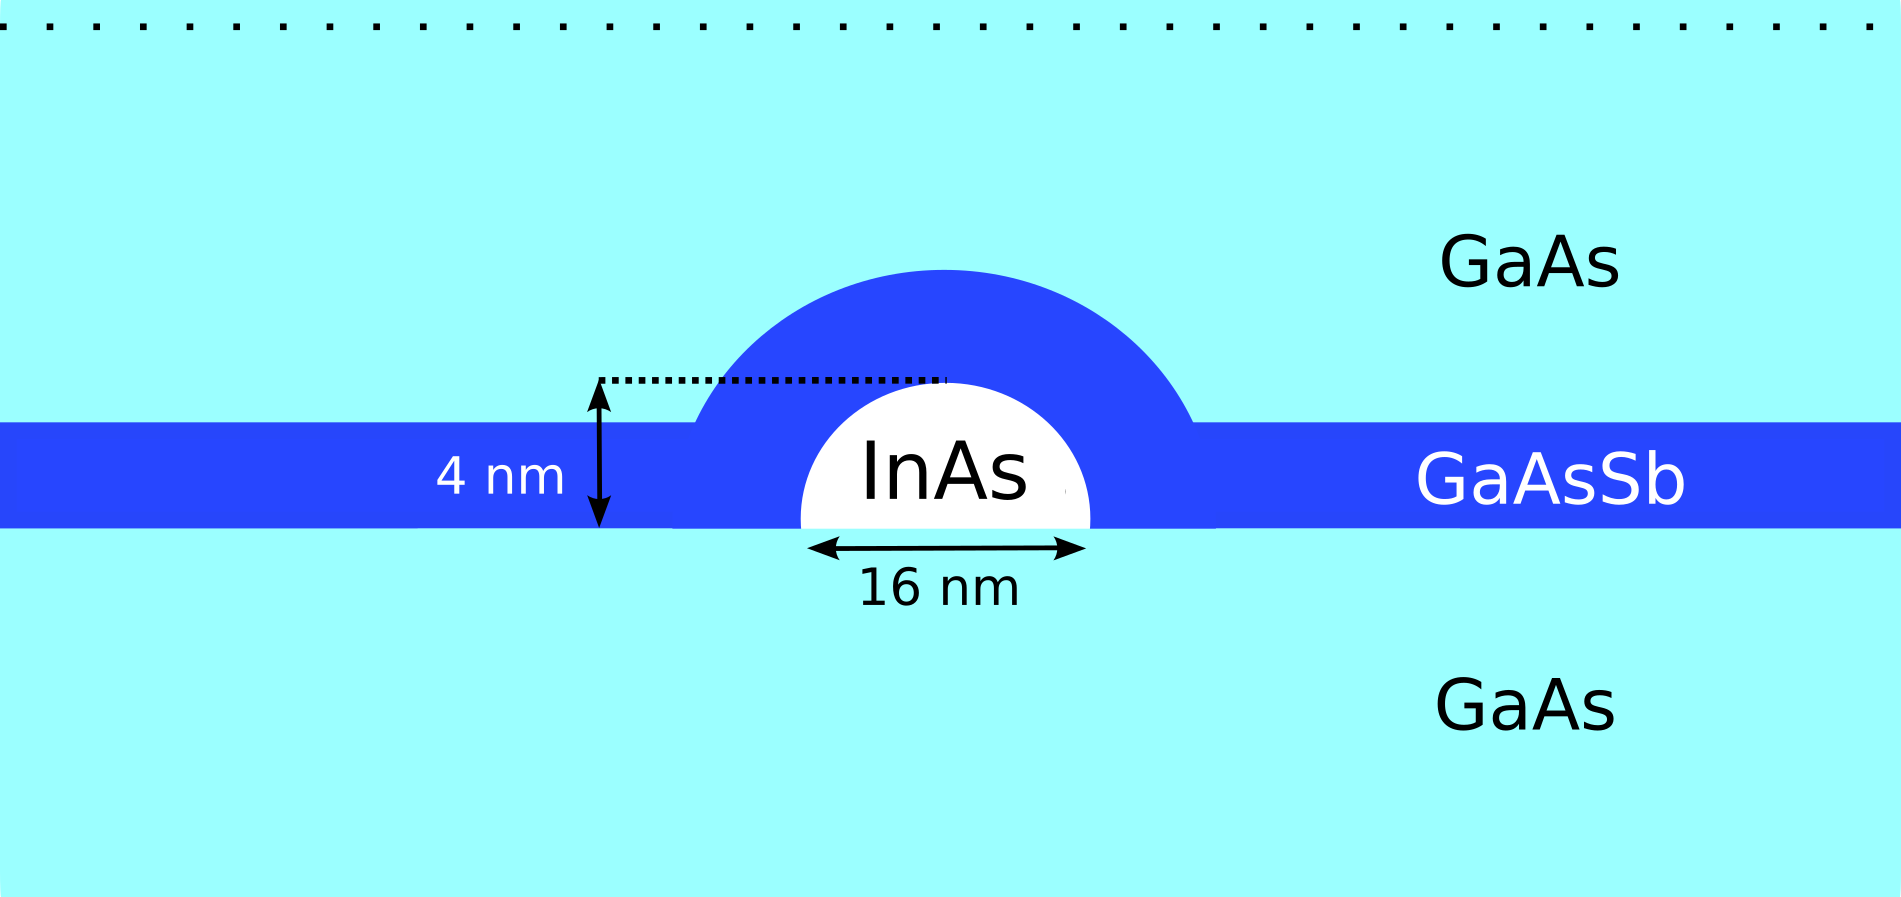
\includegraphics[width=1\linewidth]{/TEM/structure}
	\caption{Studied set of samples, $S_\mathrm{w/o}$ represents structure without QDs, $S_\mathrm{with}$ and $S_\mathrm{cap}$ are samples with In$_{1-x}$Ga$_{x}$As$_y$Sb$_{1-y}$ QDs, $S_\mathrm{cap}$ is, moreover, GaSb capped. }
	\label{fig:TUstructure}
\end{figure}

\begin{table}
	\centering
	\caption{Labels and studied sample differences.}
	%\begin{tabularx}{0.9\textwidth}{ccccc}
	\begin{tabularx}{0.95\textwidth}{ccl}
		\toprule

		%growing name & our marking& \multicolumn{3}{c}{specification}\\ 
		sample name & label& \multicolumn{1}{c}{specification}\\ 		
		\midrule
		\midrule
		%TU 12027& $S_\mathrm{w/o}$ & 5ML GaAs& &\\
		TU 12027& S$_\mathrm{w/o}$ & 5ML GaAs\\
		%TU 12040& $S_\mathrm{with}$ & 5ML GaAs,& 0.51ML In$_{1-x}$Ga$_{x}$As$_y$Sb$_{1-y}$&\\
		TU 12040& S$_\mathrm{with}$ & 5ML GaAs, 0.51~ML In$_{1-x}$Ga$_{x}$As$_y$Sb$_{1-y}$ QDs\\
		%TU 12021 & $S_\mathrm{cap}$ & 5ML GaAs,& 0.51ML In$_{1-x}$Ga$_{x}$As$_y$Sb$_{1-y}$,& GaSb cap\\
		TU 12021 & S$_\mathrm{cap}$ & 5ML GaAs, 0.51~ML In$_{1-x}$Ga$_{x}$As$_y$Sb$_{1-y}$ QDs, GaSb cap\\
		\bottomrule
	\end{tabularx}\label{tab:samples}
\end{table}

% http://nano.ceitec.cz/high-resolution-scanning-transmission-electron-microscope-fei-titan-themis-60-300-cubed/

We have studied the material composition of the sample S$_\mathrm{cap}$ by transmission electronic microscopy (TEM) with an add-on energy-dispersive X-ray (EDX) detector (SUPER-X EDX detector was used). These measurements were performed at the high resolution TEM FEI Titan Themis at CEITEC Brno. The TEM image of the whole sample and EDX emission spectrum are attached in appendix~\ref{chapter:appendix_TEM}.

In Fig.~\ref{fig:TEM}, cross-sectional TEM micrograph and graphs from parallel measured EDX for sample S$_\mathrm{cap}$ are presented. EDX spectrum is collected along the orange dashed line and averaged in the yellow boundary area. In the atomic fraction graph we show material composition in the sample as a function of horizontal position for all constituents (Ga, P, As, In, Sb). In the range between 30 and 40~nm in the cut In, As and Sb composition (elements, which are expected only in QDs area) dramatically in comparison with the concentration of 0.8~\% seen in the remainder of the sample. In the same range, we can see a decrease in phosphorus concentration at the expense of GaP. The layer where In concentration is higher than 0.8~\% we regard as QD area and its thickness is found to be of 5.8~nm with truncated-pyramid shape QDs with a base length of about 15~nm and a height of 2.5~nm. 
\begin{figure}
	\centering
	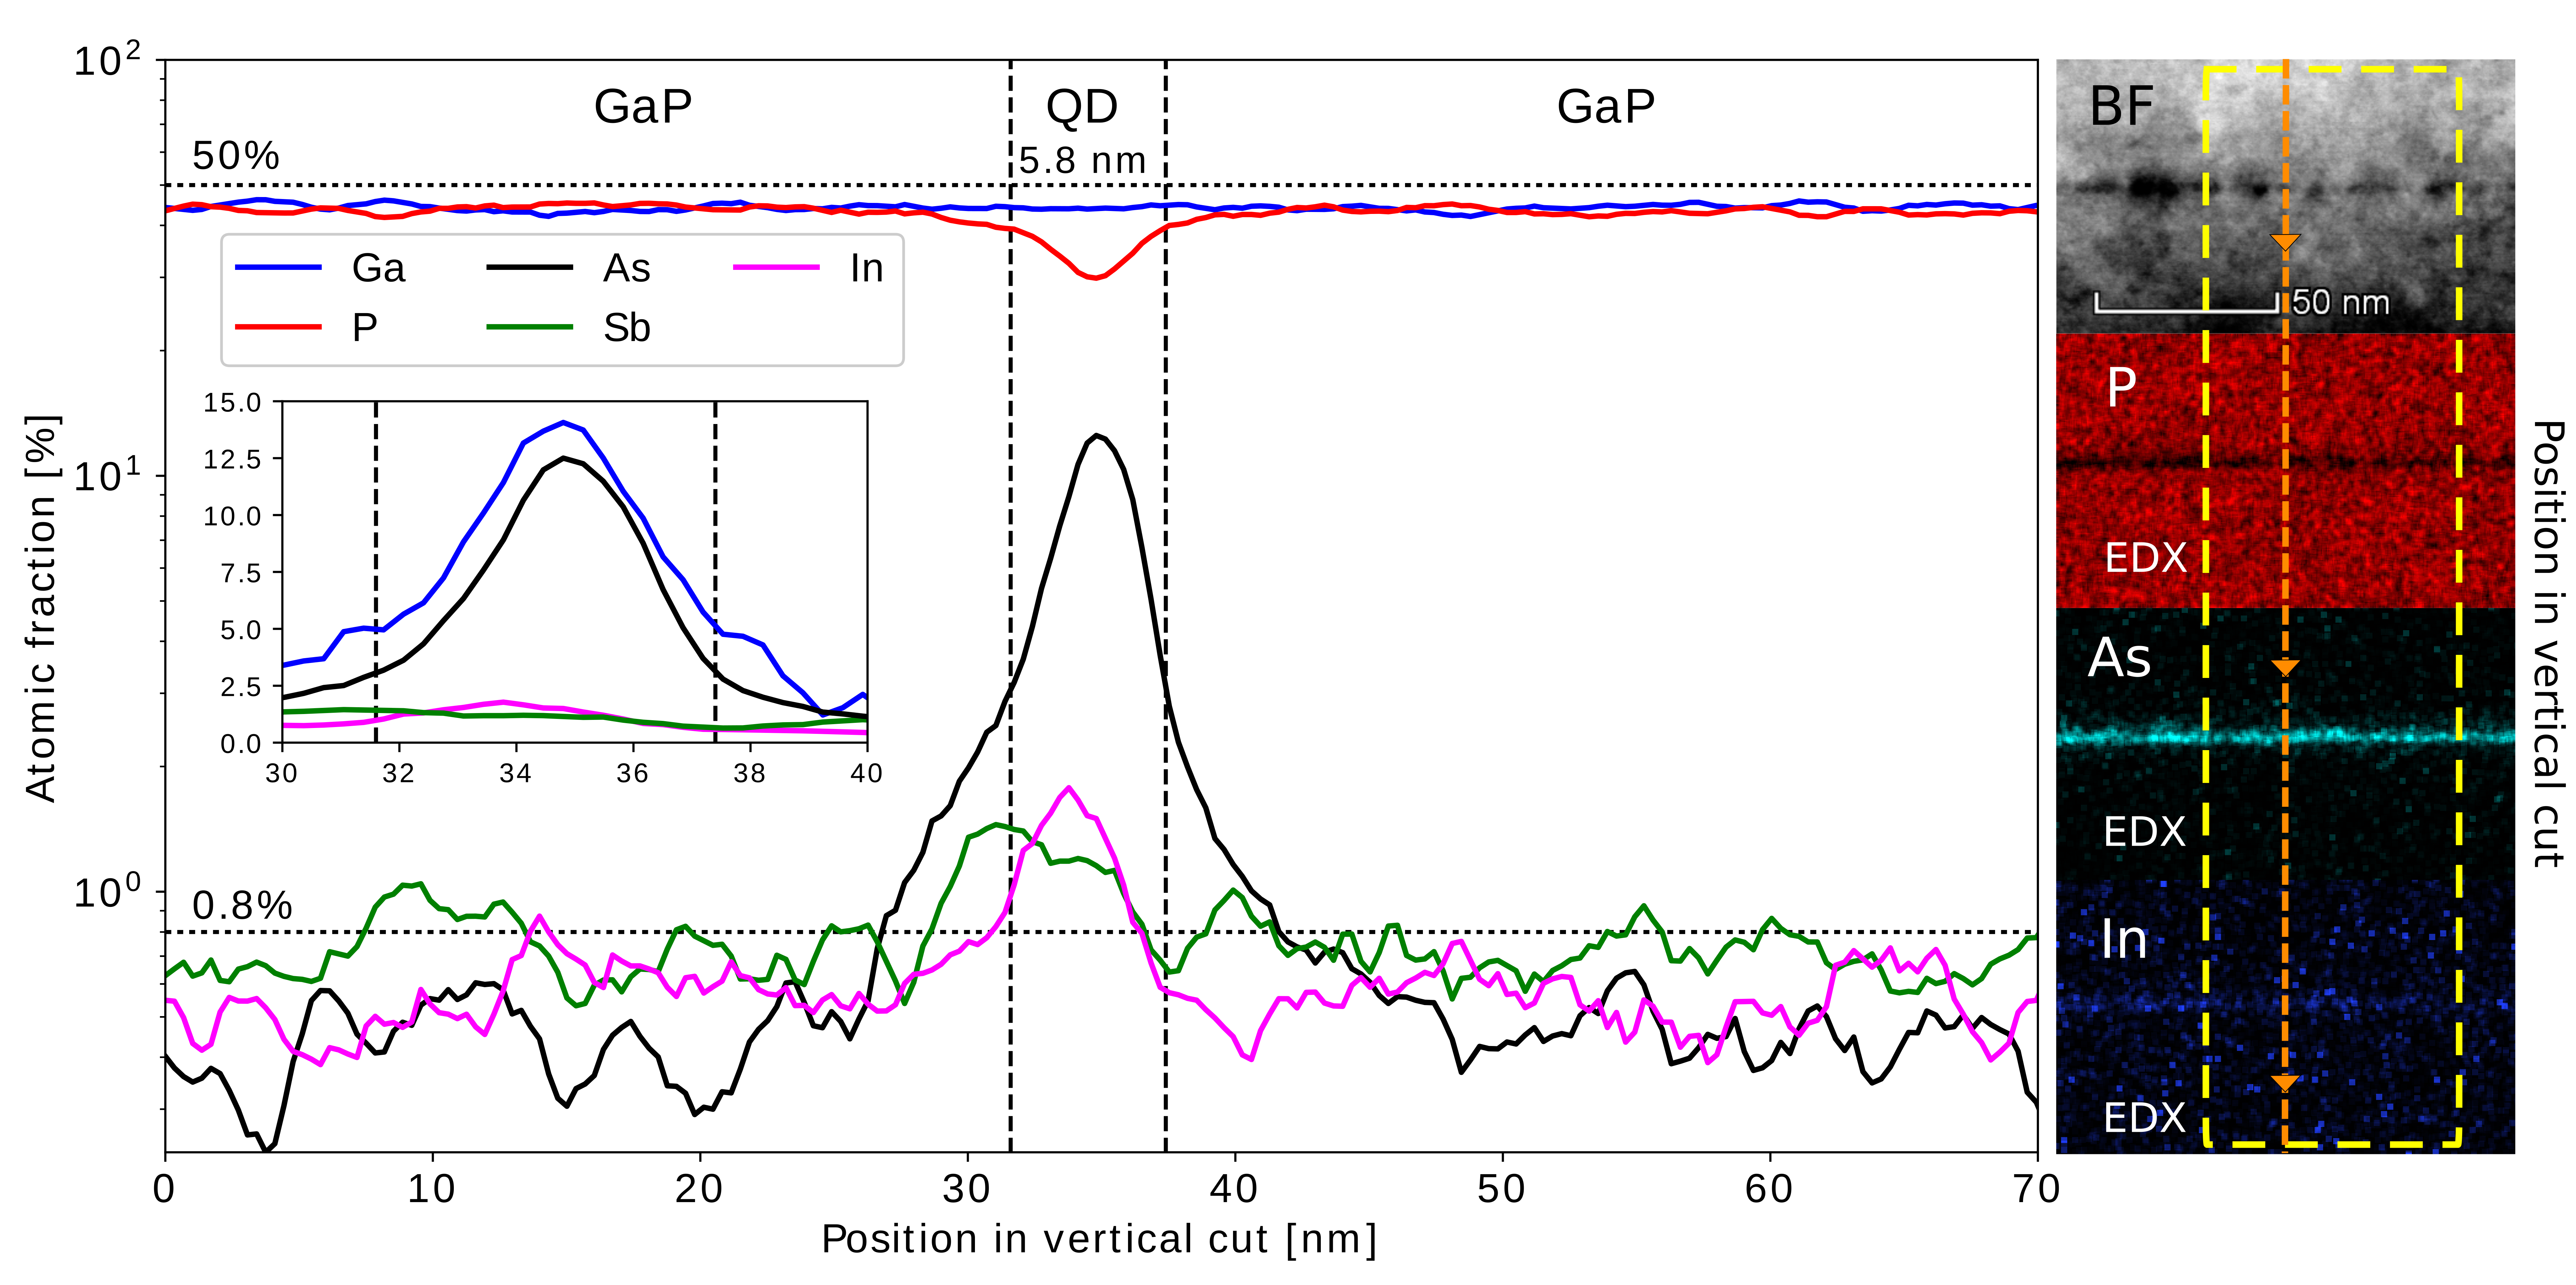
\includegraphics[width=1\linewidth]{/TEM/koncentrace_final_mapa2_QDinset}
	\caption{The atomic fraction vs. position in the vertical cut for all elements present in sample S$_\mathrm{cap}$ measured by EDX detector along the orange line in the right panel and averaged in the area circumferenced by the yellow broken curve. In QD area, i.~e., between the vertical positions of 30 and 40~nm in the cut, a substantial increase of In, As, Sb (compounds only in QD structures) and decrease of P (P is out of the QD structures) are observed. The inset shows the composition solely in the QD region. The column on right-hand side represents from top to bottom: cross-section TEM image of S$_\mathrm{cap}$ taken under strong-beam bright field condition using the (200) reflection perpendicular to the growth direction; and three EDX images measured at the same time as TEM measurements -- red one for P, white in As and purple in In.}
	\label{fig:TEM}
\end{figure}

We use the EDX data to estimate the concentration of individual elements in quaternary QD structure. Assuming that all phosphorus is bound in GaP, the concentration of Ga can be deconvoluted into Ga concentration in GaP $C_\mathrm{GaP}$ and in QD area $C_\mathrm{Ga}^\mathrm{QD}$ as
%
\begin{eqnarray}
C_\mathrm{Ga}=C_\mathrm{GaP}+C_\mathrm{Ga}^\mathrm{QD}=C_\mathrm{P}+C_\mathrm{Ga}^\mathrm{QD},
\end{eqnarray}
%
where $C_\mathrm{i}$ for $i \in \{\mathrm{Ga}, \mathrm{P}\}$ is the measured concentration of Ga and P. We assume the composition of our QDs in the form of In$_{1-x}$Ga$_{x}$As$_y$Sb$_{1-y}$, thus, we can calculate effective concetration in QD area as
%
\begin{eqnarray}
x=\frac{C_\mathrm{Ga}^\mathrm{QD}}{C_\mathrm{Ga}^\mathrm{QD}+C_\mathrm{In}^\mathrm{QD}},\qquad
y=\frac{C_\mathrm{As}^\mathrm{QD}}{C_\mathrm{As}^\mathrm{QD}+C_\mathrm{Sb}^\mathrm{QD}}.
\end{eqnarray}
%
Given the assumption that In, Ga and Sb are only in QD area, we can replace the concentration in this region with directly measured concentration by EDX. Finally, we give the estimation of $x$ and $y$ which we use in 8-band $\mathbf{k\cdot p}$ calculations of $x=84-93.5~\%$ and $y=68-91.5~\%$, see Fig.~\ref{fig:concentration_estimation}.


\begin{figure}
	\centering
	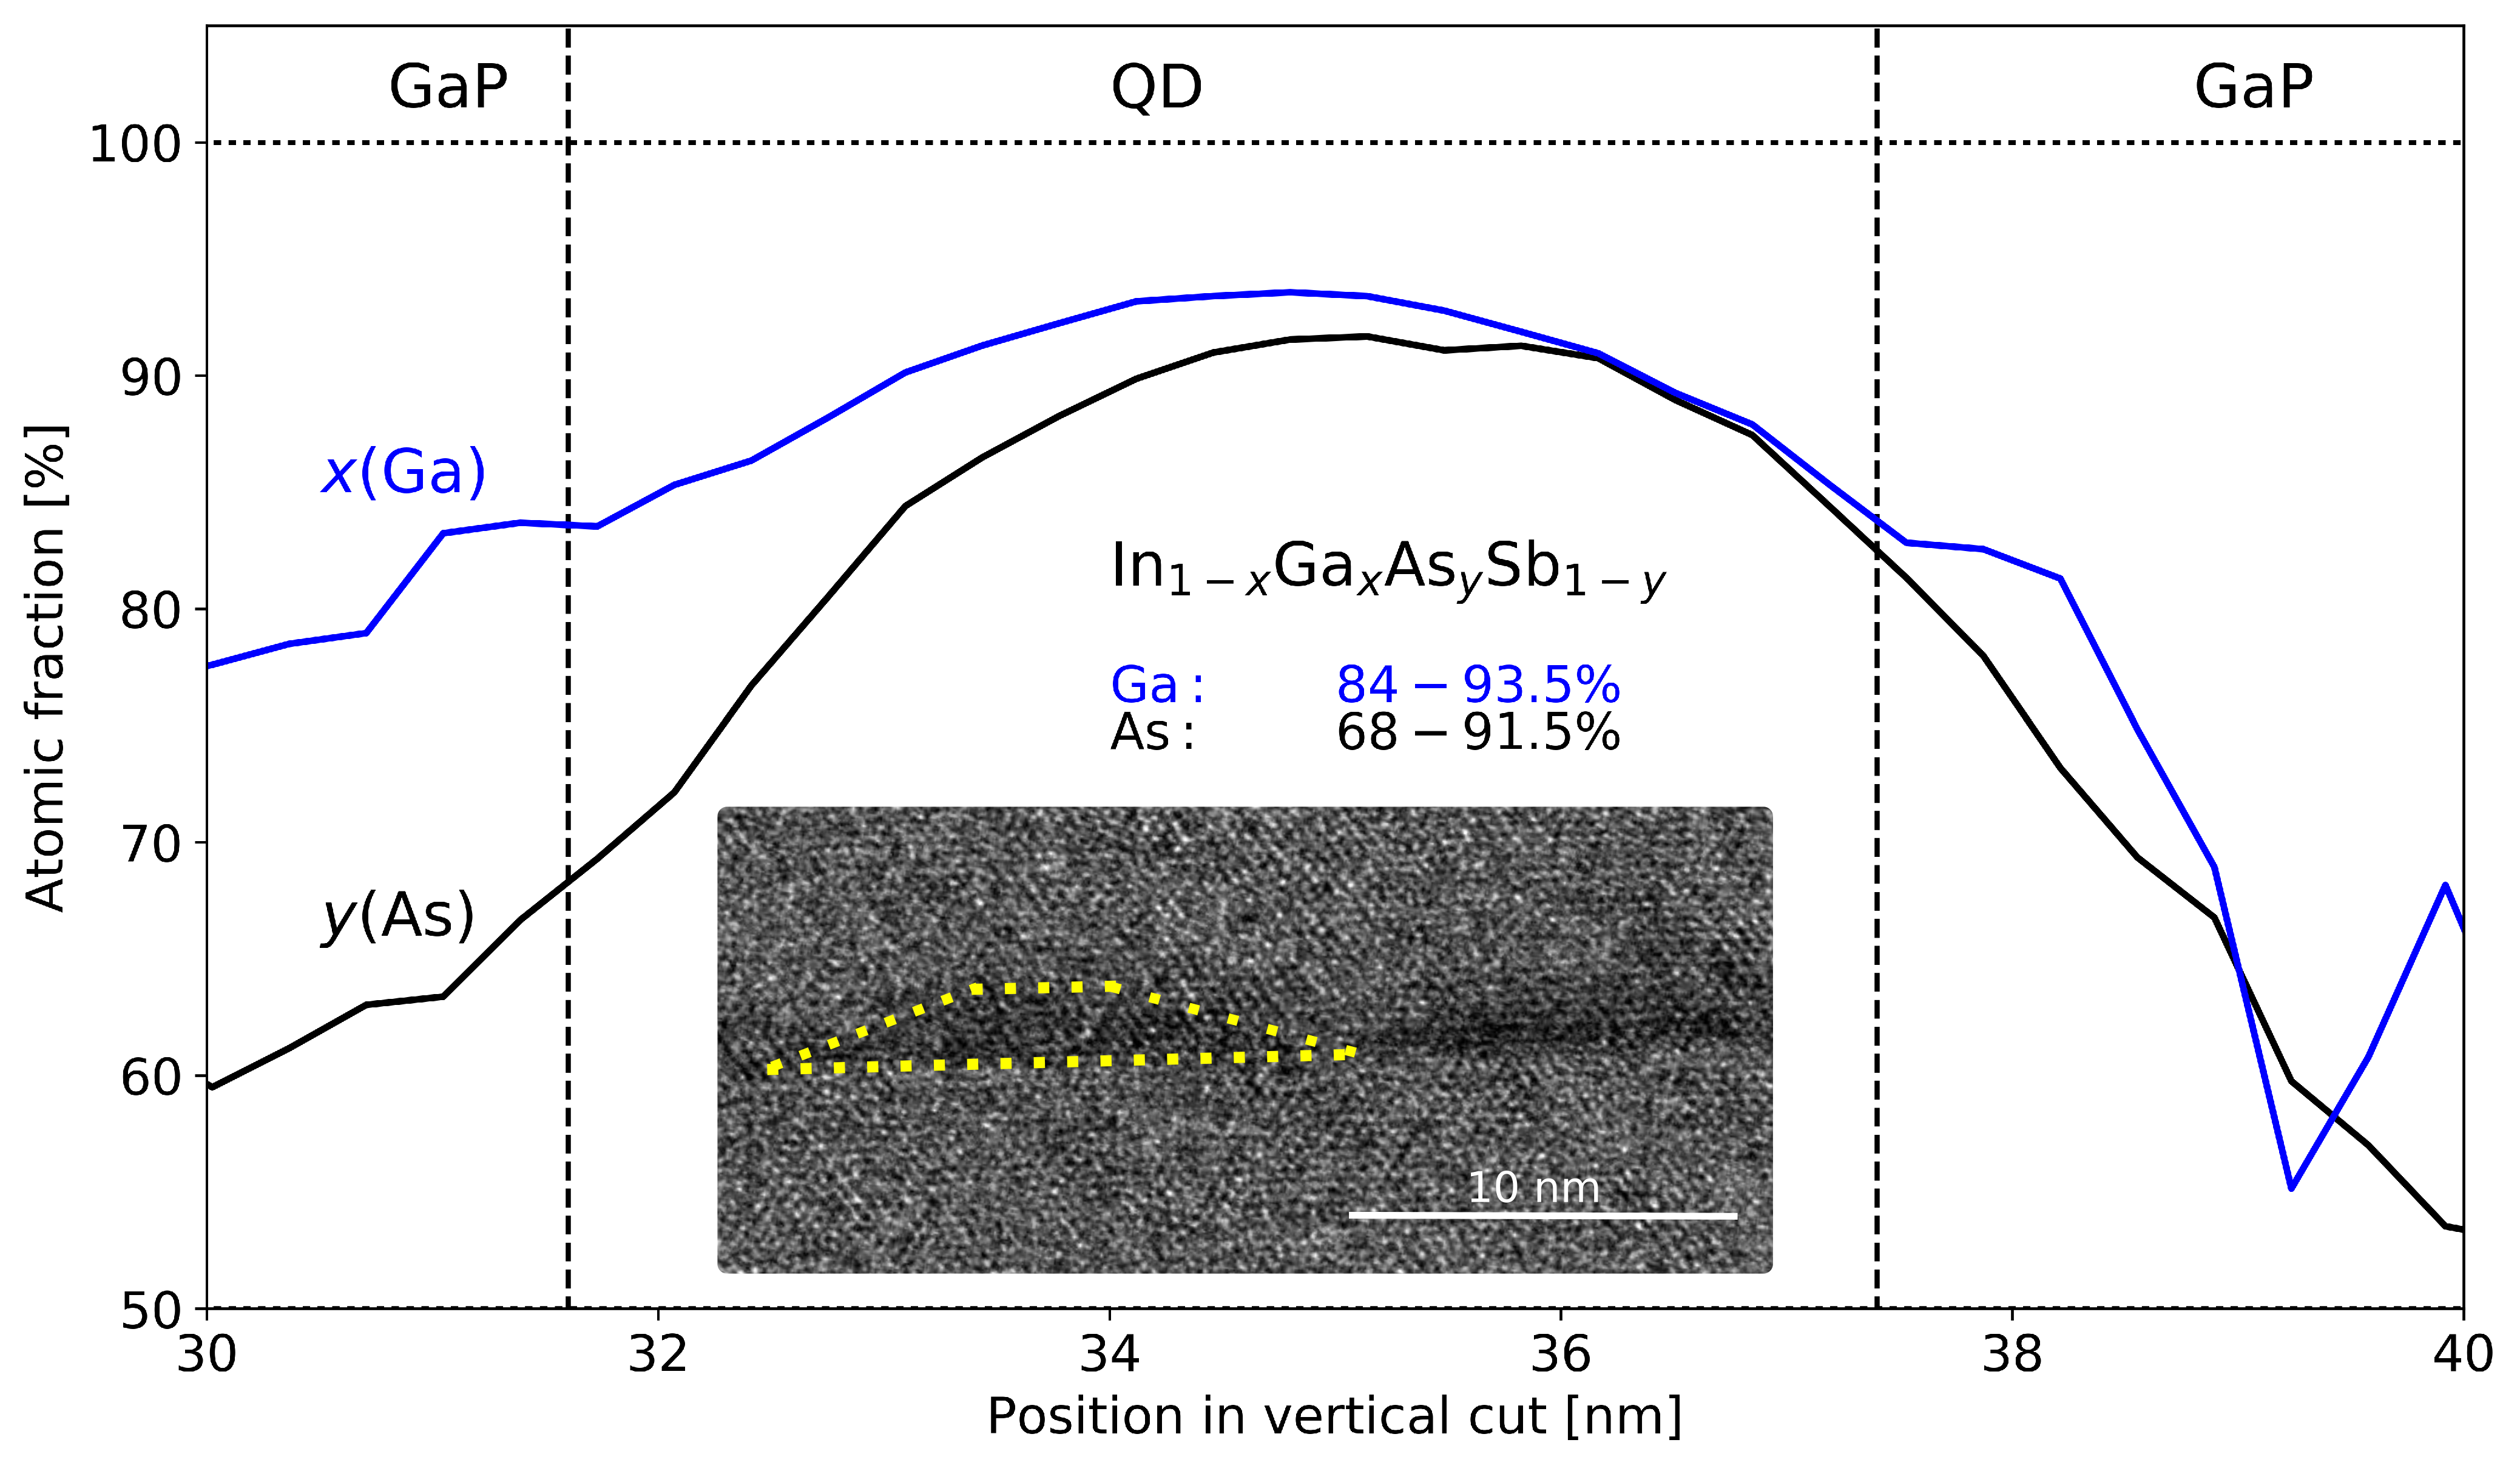
\includegraphics[width=0.85\linewidth]{/TEM/koncentrace_pro_nn} %rez_QD_konc_xy_bez}
	\caption{The estimated composition of QD area for sample S$_\mathrm{cap}$. We assume Ga and As concentration to be in the ranges of 84-93.5~\% and 68-91.5~\%, respectively. In inset we show the HRTEM image of a truncated-pyramid QD.}
	\label{fig:concentration_estimation}
\end{figure}

\clearpage

\section{Estimation of hydrostatic strain in GaAs layer}
For estimation of a hydrostatic component of the strain was performed room temperature Raman measurements of our samples. These measurements were obtained using NT-MDT spectrometer with a 100$\times$/0.7~NA long working length objective and the 532~nm laser. The scattered light was dispersed using a 1800~groove/mm grating and detected by a thermoelectrically cooled Si CCD camera. The spectra were recorded in $z(xy)z$ backscattering geometry.

Measured signals were fitted by the sum of 3 Lorentzian curves.
Let we focus to Raman signal around 290~cm$^{-1}$ where the TO phonon of strained GaAs QWs for our QDs samples is expected. Fig.~\ref{fig:raman} reports about $\sim$19~cm$^{-1}$ shift of TO phonon for our QDs samples compared to bulk material. Using a model~\cite{Montazeri_Nano2010}, we can use the shift to estimate the value of hydrostatic strain $\epsilon_{xx}$ 
\begin{equation}
k_\mathrm{TO}^2 = k_\mathrm{TO,B}^2 + (p+2q)\epsilon_{xx},
\end{equation}
where $k_\mathrm{TO}$ and $k_\mathrm{TO,B}$ are the Raman shifts of TO GaAs mode of strained and bulk GaAs, and $p$ and $q$ are phonon deformation potentials taken from Ref.~\cite{Cerdeira_PRB1972}.

The measured shifts of TO mode of $S_\mathrm{w/o}$ correspond to $\epsilon_{xx}=-0.032$, of $S_\mathrm{with}$ to $\epsilon_{xx}=-0.026$,  and for $S_\mathrm{cap}$ is $\epsilon_{xx}=-0.030$, which is in good agreement with the predicted hydrostatic strain component $\epsilon_{xx}=-0.034$ by the $\mathbf{k \cdot p}$ calculations, see Fig.~\ref{fig:raman_theory_wo}. %approximately three times less than predicted hydrostatic strain component by the $\mathbf{k \cdot p}$ calculations, see Fig.~\ref{fig:raman_theory_wo}.
\begin{figure}
	\centering
	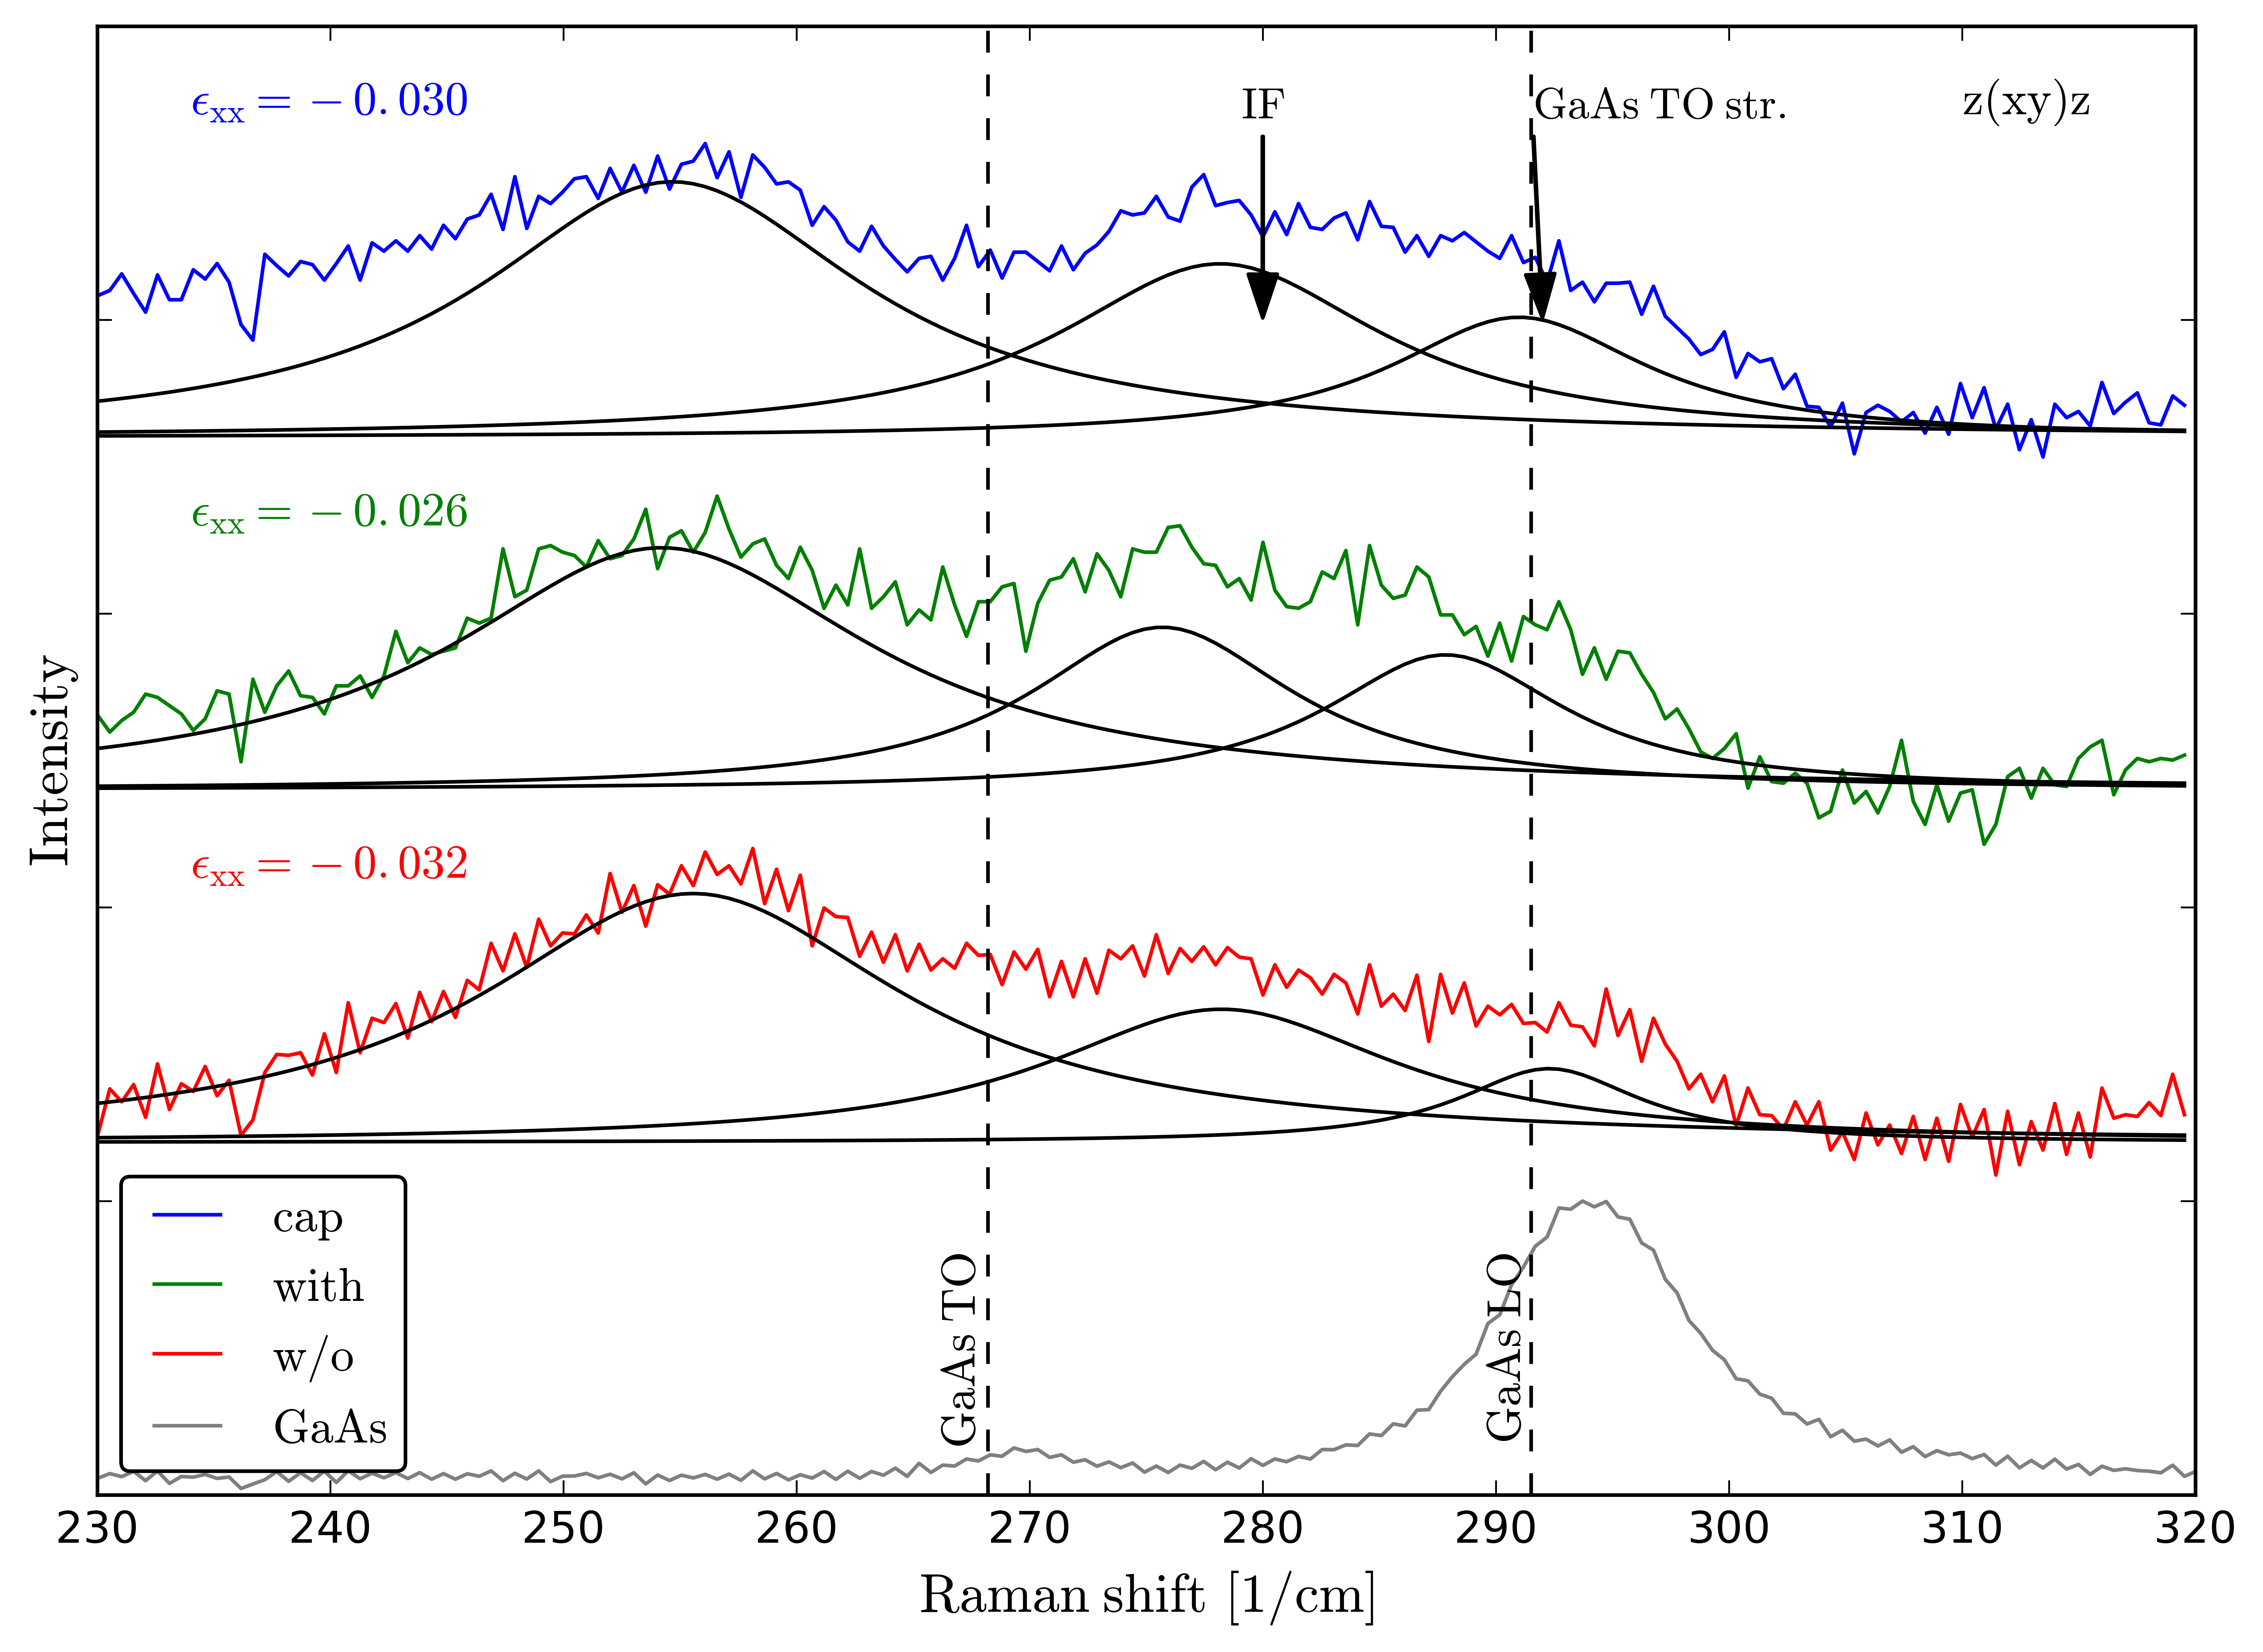
\includegraphics[width=0.85\linewidth]{/raman/Raman_TUB_and_GaAs_enlg_230_to_320_fit}
	\caption{Raman spectra of samples w/o QDs $S_\mathrm{w/o}$ (red), with QDs $S_\mathrm{with}$ (green) and capped QDs $S_\mathrm{cap}$ and bulk GaAs (grey). The dashed lines show reference GaAs TO and LO modes~\citep{Esther_Nanotech2013}. Calculated hydrostatic strain components $\epsilon_{xx}$ are presented in inset of the figure. A label IF corresponds to interface Raman band.}
	\label{fig:raman}
\end{figure}

\begin{figure}
	\centering
	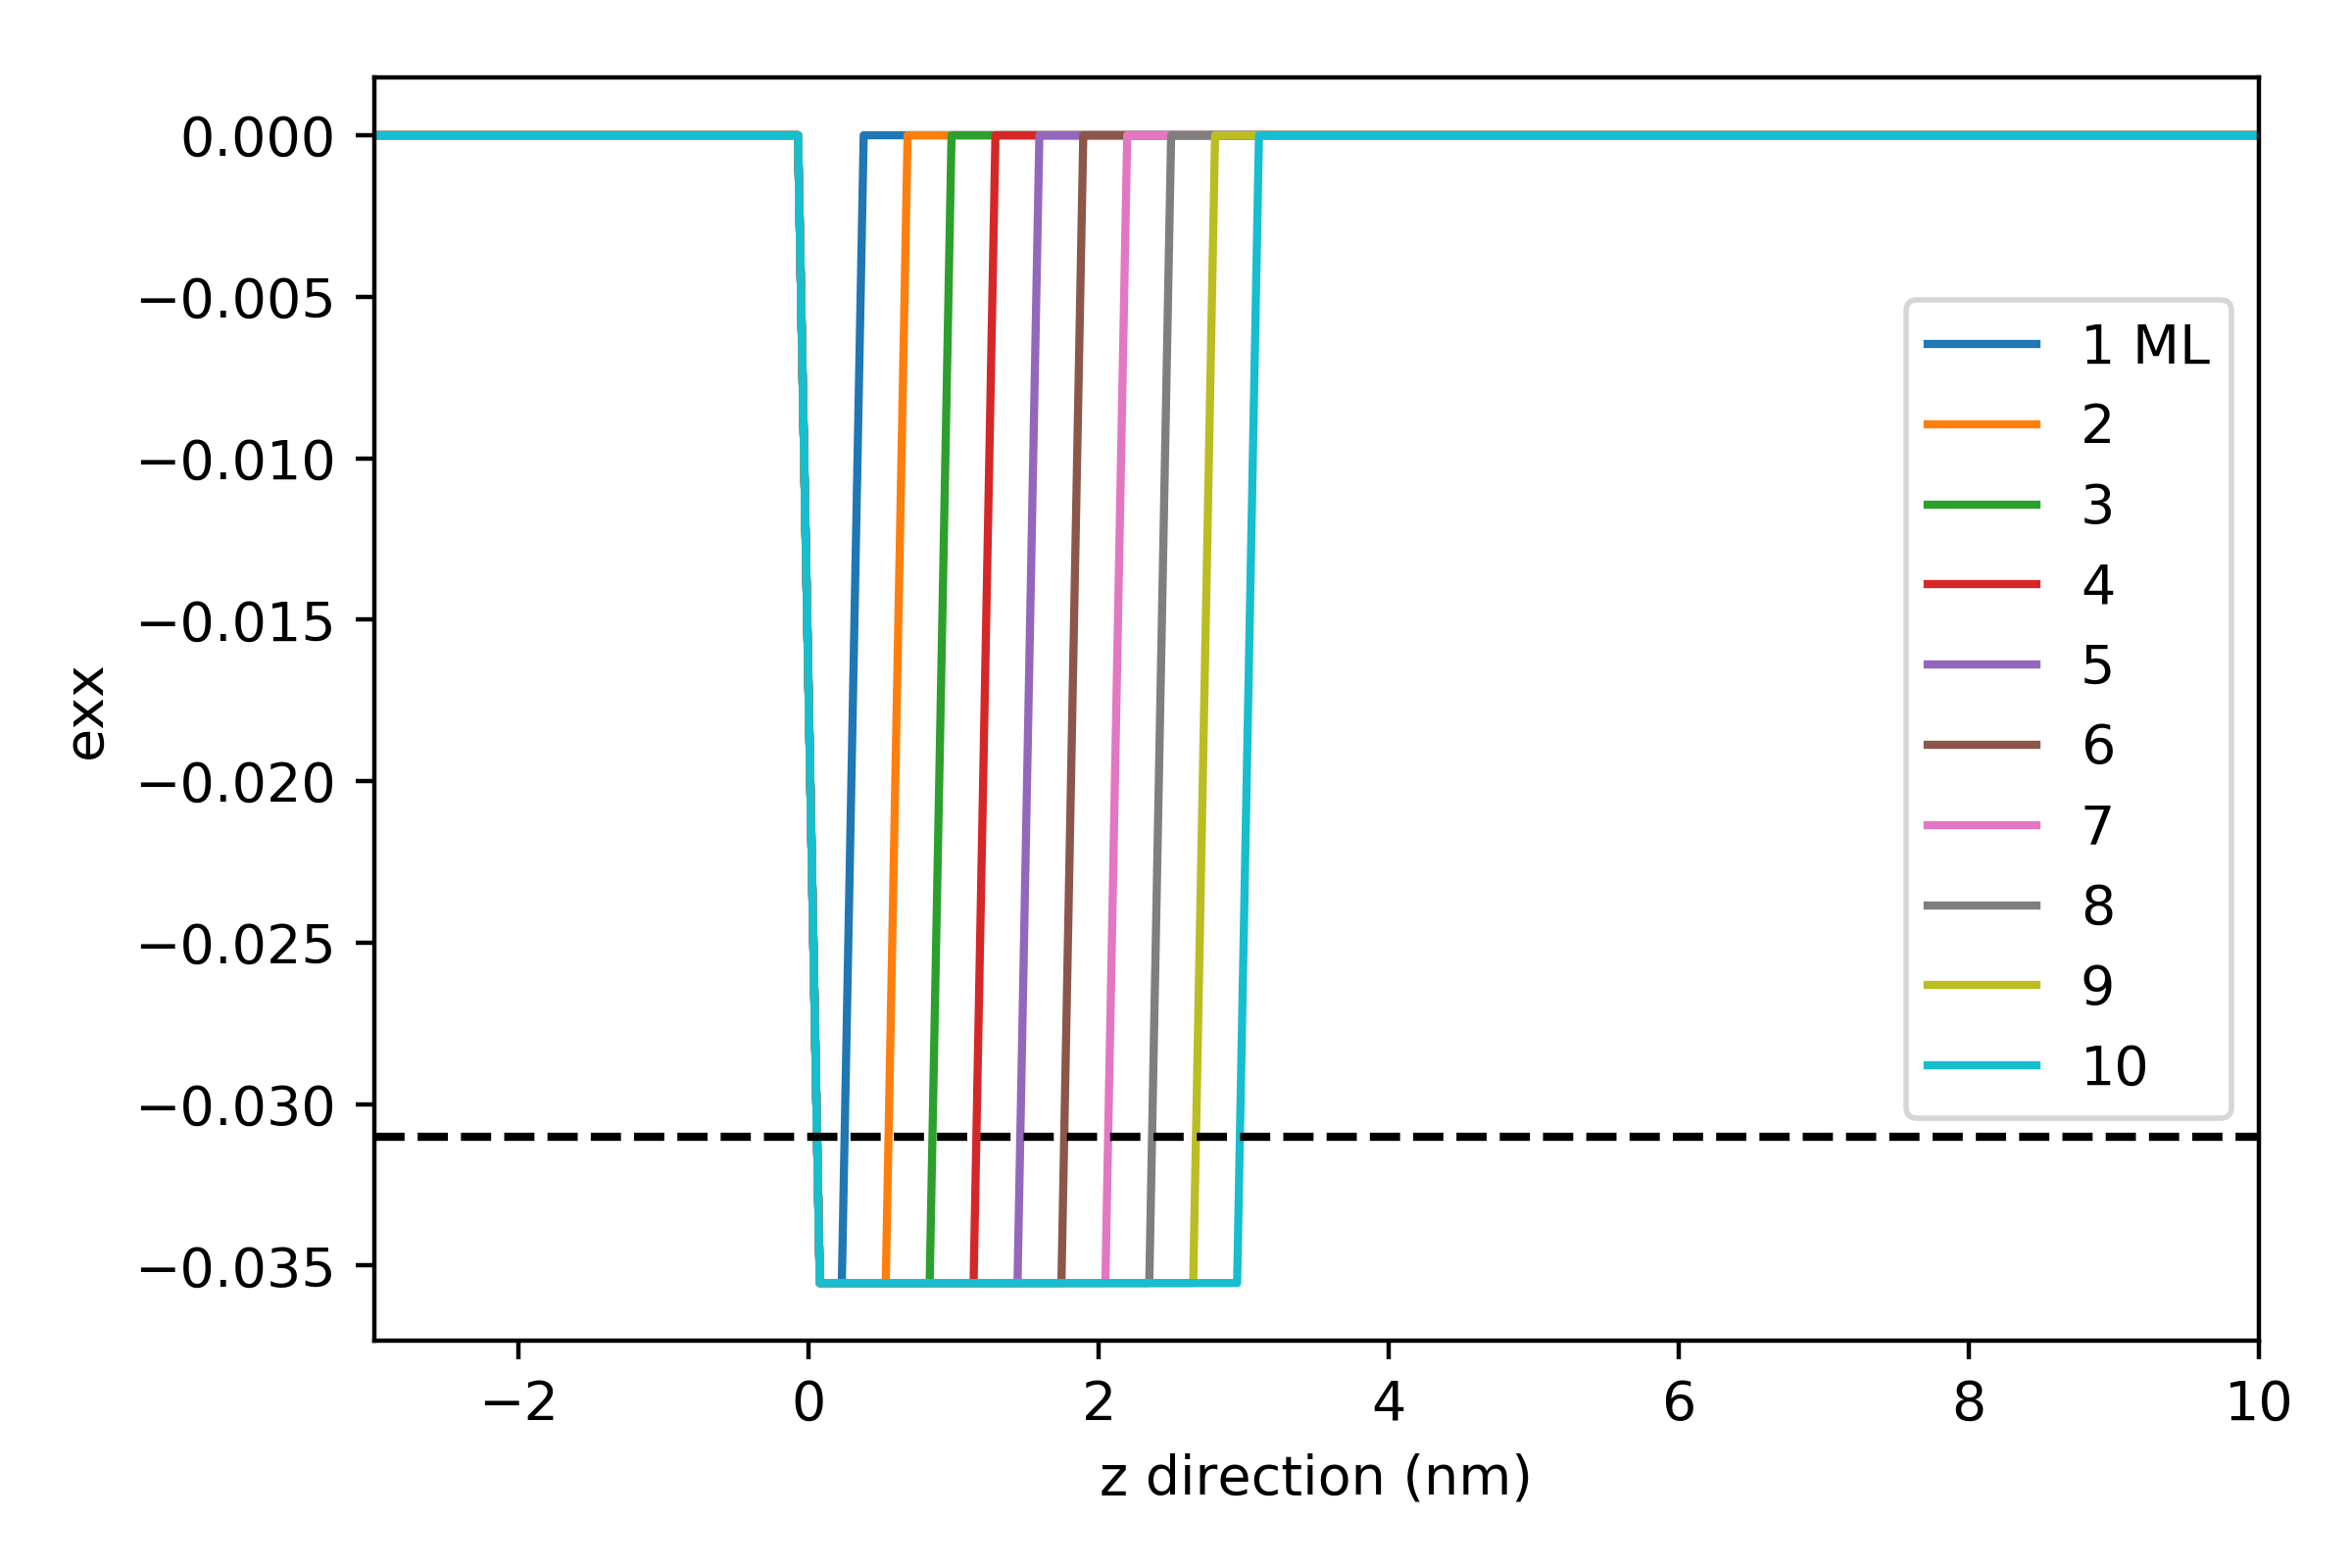
\includegraphics[width=0.85\linewidth]{/raman/eyy_vs_ML}
	\caption{Hydrostatic strain $\epsilon_{xx}$ calculated as a function of GaAs layer thickness in the sample $S_\mathrm{w/o}$. The experimental value is represented by a dashed curve. The calculations were made by the supervisor.}
	\label{fig:raman_theory_wo}
\end{figure}


\clearpage
\section{Experimental setup for photoluminescence measurements}
The PL measurements were performed using standard PL setup. The samples were positioned in the cryostat, cooled to 15~K and pumped by a laser diode with the wavelength of 405~nm with 0.05~mm$^2$ large spot size. The emitted emission signal was dispersed by a 1200~grooves/mm ruled grating designed to the wavelength of 750~nm and synchronously detected by a Si-avalanche photodiode (APD). We have performed the following PL experiments: (i) in intensity dependent measurements the laser power was varied by a neutral density (ND) filter over more than 4 orders of magnitude, (ii) in the temperature resolved PL temperature was changed from 15~K to room temperature, but for our samples and given integration time (0.3~s per one wavelength) we have not detected any PL signal at 300~K, (iii) the polarization of the PL was analyzed by a rotating achromatic half-wave retarder followed by a fixed linear polarizer.

In time-resolved experiments we have used laser with wavelength of 405~nm focused on 0.06~mm$^2$ area with pulse-width of 60~ps; emitted PL spectrum was dispersed again by 1200~grooves/mm ruled grating and detected by a Si-APD. We have performed the following TRPL experiments: (i) intensity resolved TRPL was measured at 15~K in 200~ns temporal window with resolution around 800~ps; the pumping power density was tuned by a ND filter in a range of 0.1--0.7~W/cm$^2$. The repetition rate of the laser was 5~MHz. (ii) In temperature resolved TRPL a temperature was changed on a range 15--150~K, the temporal window was modified to maximize the resolution from 200~ns for lower temperature to 25~ns for higher temperature. Tuning the temporal window is connected with changes in repetition rate, which was varied between 5 (for the temporal window 200~ns) and 80~MHz (for 25~ns).

Both experimental setups are schematically depicted in~\ref{fig:Madrid_setup}.
\begin{figure}
	\centering
	\includegraphics[width=1\linewidth]{/PL/setup}
	\caption{Schematic of the (a) PL and (b) TRPL measurement setup. The picture of the TRPL setup is motivated by Ref.~\citep{TRPL_setup}.}
	\label{fig:Madrid_setup}
\end{figure}


\newpage
\section{Photoluminescence measurements}

The homogeneity of samples was tested by performing PL measurements on different areas of them. The results of those for different samples spots (distinguished by the type of the curve) and samples (different color) are depicted in the Fig.~\ref{fig:PL_homogenity}. We can see that samples are rather spatially homogeneous, hence our measurements might be considered as reproducible on the samples. %it is not necessary measured PL and TRPL in the same time. 

Let look at the emission structures around 1.8~eV. Firstly, we compare substrate emission in this spectral range with signal from our samples. We clearly see a broader band which is around 70~times smaller than emission from our samples so that we neglect this band. For $S_\mathrm{w/o}$ are shown PL with two maxima located at 1.83 and 1.86~eV, respectively. The PL signal of samples with QDs are shifted to smaller energies: the maxima are located at 1.78~eV for $S_\mathrm{with}$ and 1.74~eV for $S_\mathrm{cap}$. Finally, let us notice that the PL from $S_\mathrm{with}$ is twice stronger compared to other samples.
\begin{figure}
	\centering
	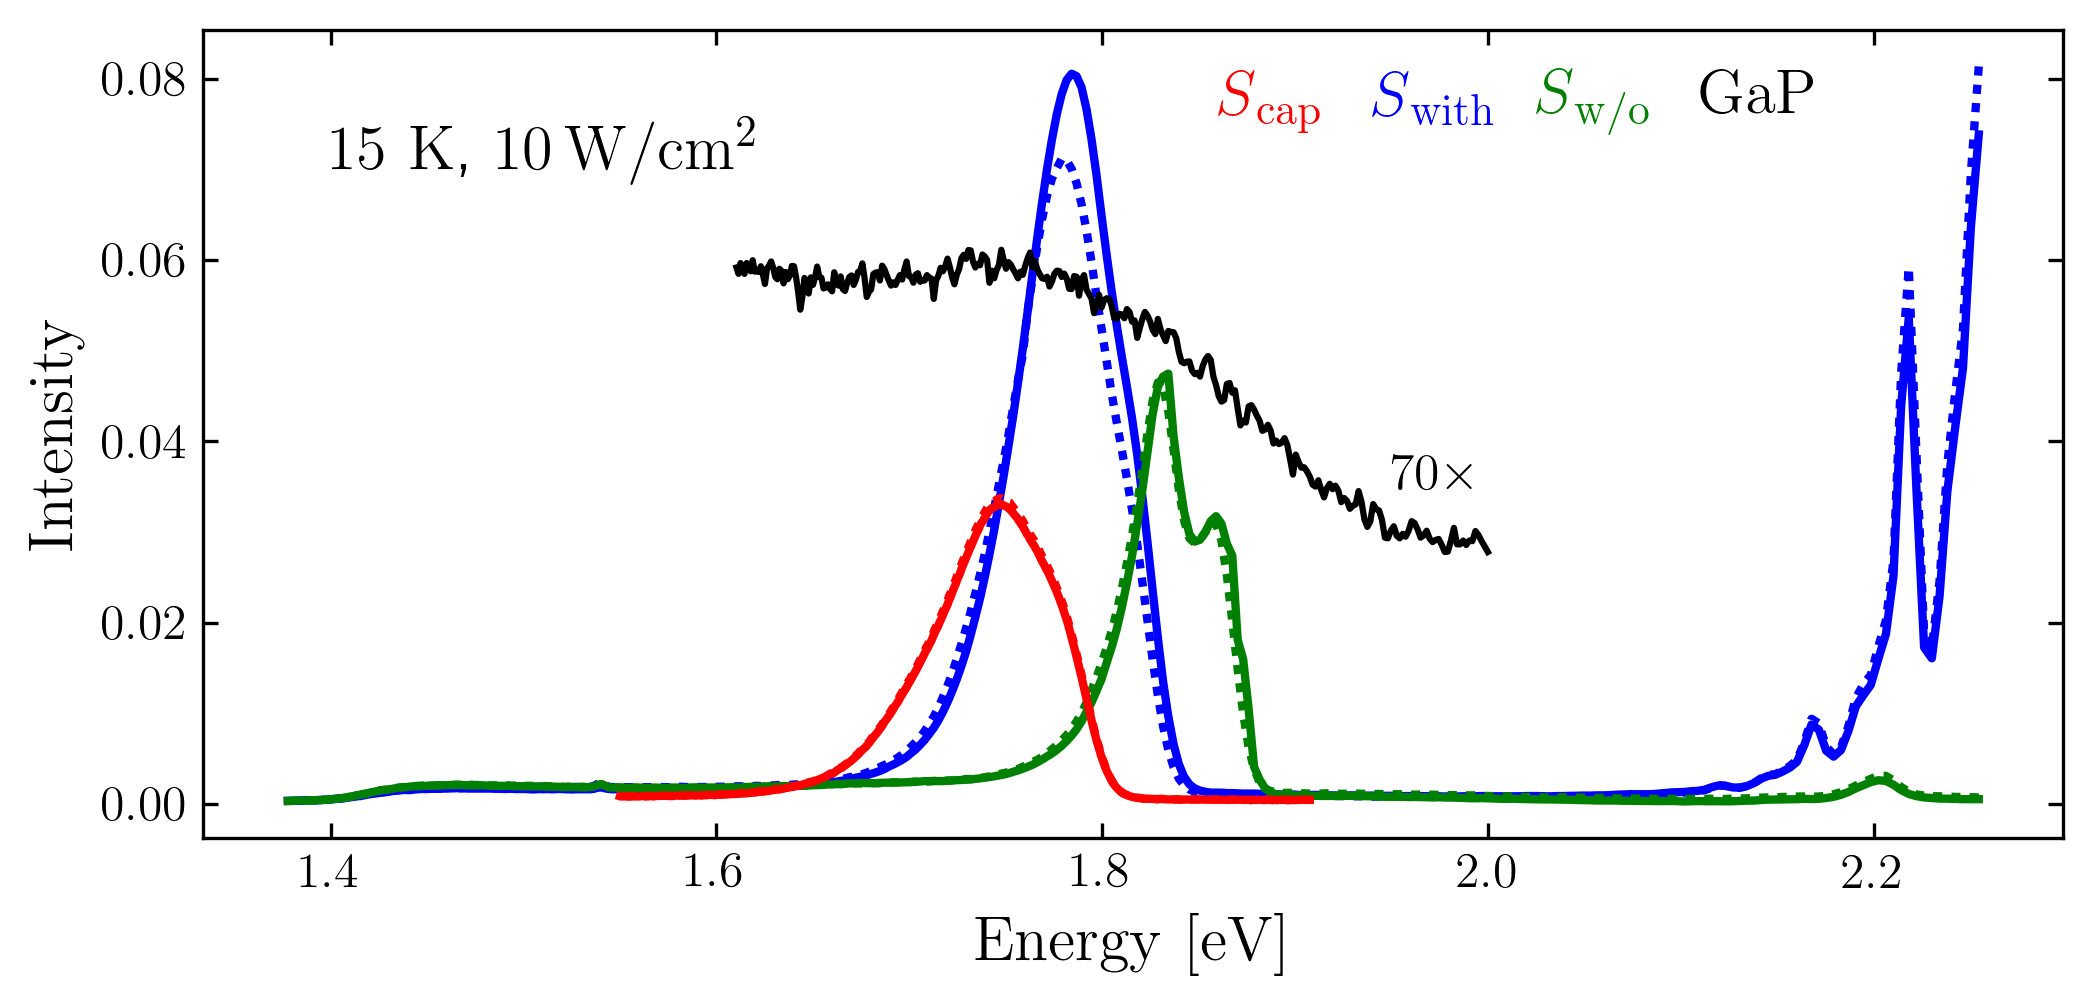
\includegraphics[width=1\linewidth]{/PL/all__IntensityVSen_GaP}
	\caption{PL for samples $S_\mathrm{w/o}$ (green lines), $S_\mathrm{with}$ (blue) and $S_\mathrm{cap}$ (red) measured at 15~K and 10~W/cm$^2$ on several places on samples (different curve types). PL from our samples is compared with emission from GaP substrate (black).}
	\label{fig:PL_homogenity}
\end{figure}

\subsection{Excitation intensity dependent PL}
\label{sec:intensity_PL_TU}
PL for each sample and excitation density $D$ was fitted by sum of three Gaussian curves and the individual bands corresponding to different optical transitions was studied. 

\subsubsection*{Sample without QDs $\mathbf{S_\mathrm{w/o}}$}

\begin{figure}
	\centering
	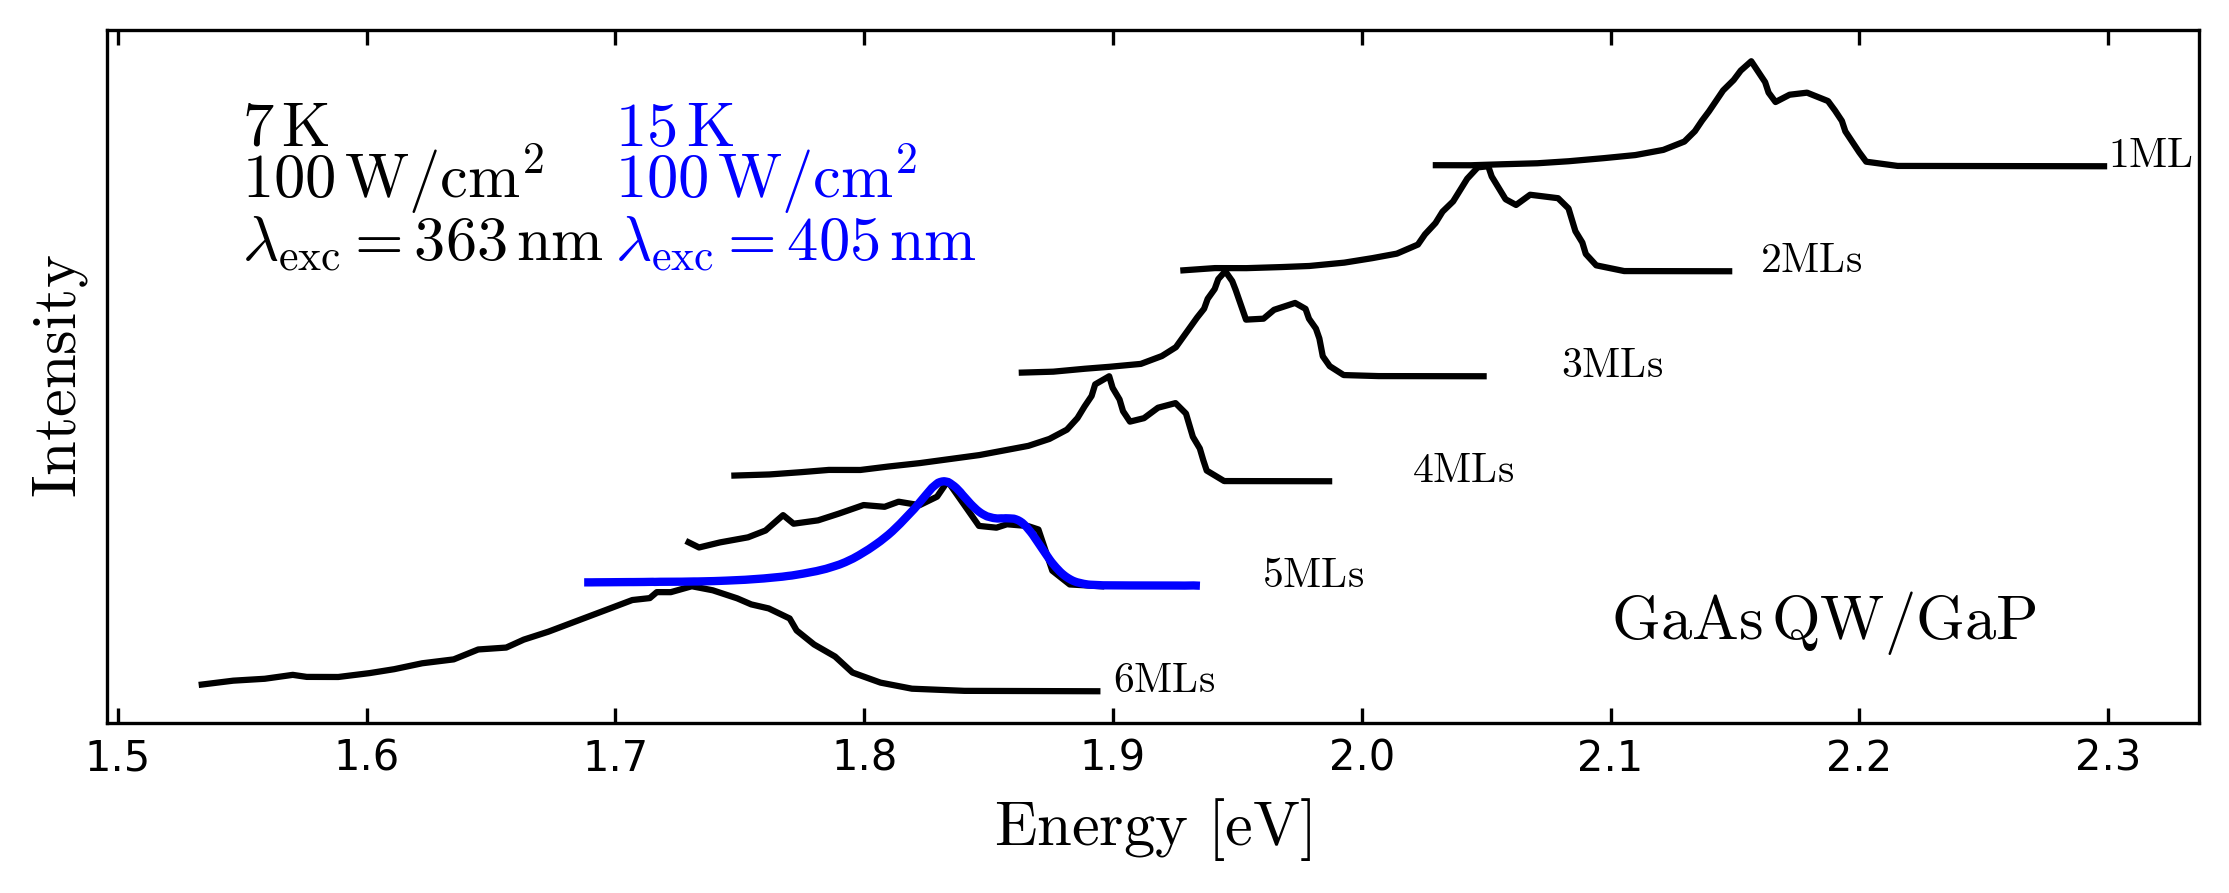
\includegraphics[width=0.9\linewidth]{/PL/12027_ref_GaAs_5ML_new}
	\caption{The comparison of the spectrum of $S_\mathrm{w/o}$ (blue) with set of samples with variable thickness taken from~Ref.~\citep{Prieto_APL1997} (black). The measurement temperature of 15~K (7~K), excitation wavelength of 405~nm (363~nm) in our (in ref.~\citep{Prieto_APL1997}) were used. Excitation density in both experiments was 100~W/cm$^2$. We can see a good match of sample $S_\mathrm{w/o}$ with 5ML thick GaAs QW from Ref.~\citep{Prieto_APL1997}.}
	\label{fig:12027_ref}
\end{figure}


\begin{figure}
	\centering
	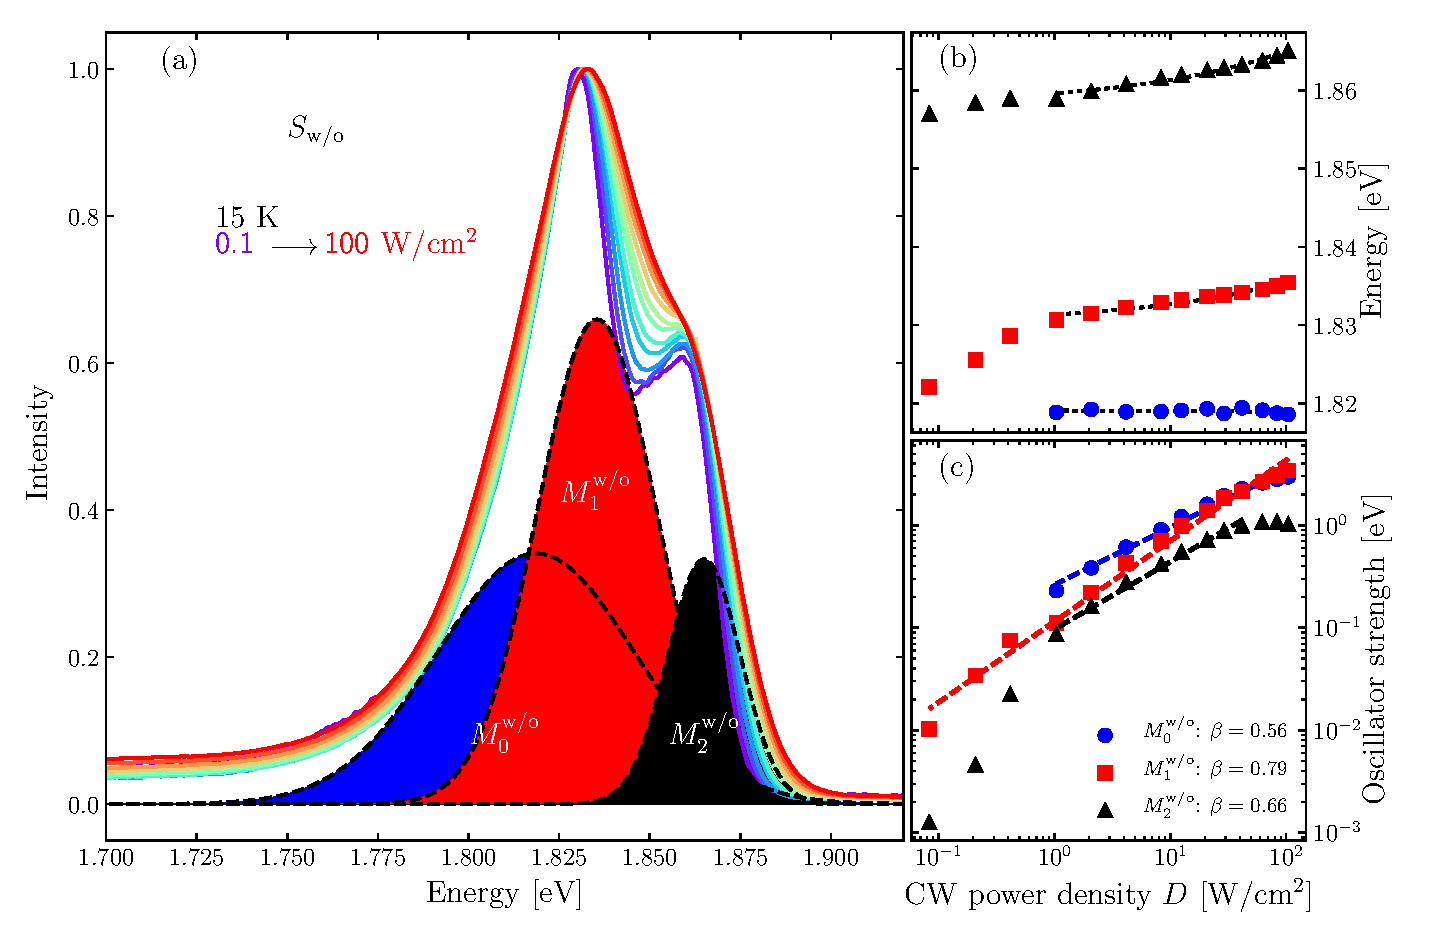
\includegraphics[width=0.9\linewidth]{/PL/intensity/12027_11011_norm_PL_int}
	\caption{(a) PL spectra of $S_\mathrm{w/o}$ measured for several excitation density in the range 0.1 and 100~W/cm$^2$. The fit by the sum of three Gaussian curves is shown for 100~W/cm$^2$ and the individual bands are presented by shaded area: $M_0^\mathrm{w/o}$ (blue), $M_1^\mathrm{w/o}$ (red) and $M_2^\mathrm{w/o}$ (black). In (b) we show power dependence of the energy of individual bands and their fits by Eq.~\ref{eq:PL_intmodel} (dotted curves). Panel (c) depicts the oscillators strength of the bands in log-log scale and their fits by linear lines (broken lines), respectively. The slopes of the linear fit $\beta$ (exponent in linear scale) are presented in the legend of panel (c). Individual transitions in panels (b) and (c) are represented by: $M_0^\mathrm{w/o}$ (blue circles), $M_1^\mathrm{w/o}$ (red squares) and $M_2^\mathrm{w/o}$ (black triangles).}
	\label{fig:QD_wo_int}
\end{figure}
Three emission bands of sample $S_\mathrm{w/o}$ labelled from smaller to greater localization energy $M_0^\mathrm{w/o}$, $M_1^\mathrm{w/o}$ and $M_2^\mathrm{w/o}$, respectively, are related to electrons in the $X_{xy}$ (the $X$ bands for GaAs strained to GaP are split into $X_z$ and $X_{xy}$ where $z$ indicates growth direction) GaAs minima recombination with heavy holes in the $\Gamma$ band in GaAs layer. Ref.~\citep{Prieto_APL1997} discusses the effect of GaAs layer thickness on emission spectra where they observed overally an energy shift, with the thickness of the layer, but the energy separations between corresponding bands stayed nearly independent of layer thickness. Similarly as in Ref.~\citep{Prieto_APL1997}, where those were 12 and 32~meV, we detect similar ones and depending on the excitation density we have found them to be between 12--17~meV and 40--46~meV. Hence, the peaks cannot be attributed to thickness fluctuations, but instead they can be connected with phonon-assisted transitions. The energies of the phonons closely correspond to TA and LA phonon energies in GaP~\citep{Prieto_APL1997}. In Fig.~\ref{fig:12027_ref} PL of $S_\mathrm{w/o}$ is compared with studied set taken from Ref.~\citep{Prieto_APL1997}.



In Fig.~\ref{fig:QD_wo_int}(a) we show PL spectra of the sample with increasing $D$ and their deconvolution into individual band by Gaussian fits. The energy-shift is visualized in Fig.~\ref{fig:QD_wo_int}(b), where PL peak energies as a function $D$ for individual bands are plotted and fitted with usually used formula~\citep{Hatami_apl1995_intmodel,Glaser_apl1996_intmodel,Ledentsov_prb1995_intmodel} derived for spatially indirect optical transition in quantum wells (QWs) and QDs
%
\begin{equation}
E(D)=E_\mathrm{I}+\gamma D^{1/3}, \label{eq:PL_intmodel}
\end{equation}
%
where $E_\mathrm{I}$ is extrapolation energy to $D=0$~W/cm$^2$ and $\gamma$ is proportional constant which describes the gradient of the energy-shift. The energy evolutions of the bands are well characterized with~Eq.~(\ref{eq:PL_intmodel}). The bands $M_1^\mathrm{w/o}$ and $M_2^\mathrm{w/o}$ are slightly shifted to blue with increasing $D$, these blue-shifts are described by almost identical $\gamma$, whereas $M_0^\mathrm{w/o}$ is rather independent on $D$ or slightly red-shifted.






The oscillator strengths in Fig.~\ref{fig:QD_wo_int}(c) of $M_0^\mathrm{w/o}$, $M_1^\mathrm{w/o}$ follow a linear dependence in log-log graph with the excitation power in the whole measured range, indicating that there is neither saturation of electronic states nor the activation of the non-radiative events. The emission of $M_2^\mathrm{w/o}$ is linear only in the power density range 1 and 30~W/cm$^2$, under the range PL is saturated.

%%%%%%%%%%%%%%%%%%%%%%%%%%%%%%%%%%%%%%%%%%%%%%%
\subsubsection*{Sample with QDs $\mathbf{S_\mathrm{with}}$}
\begin{figure}
	\centering
	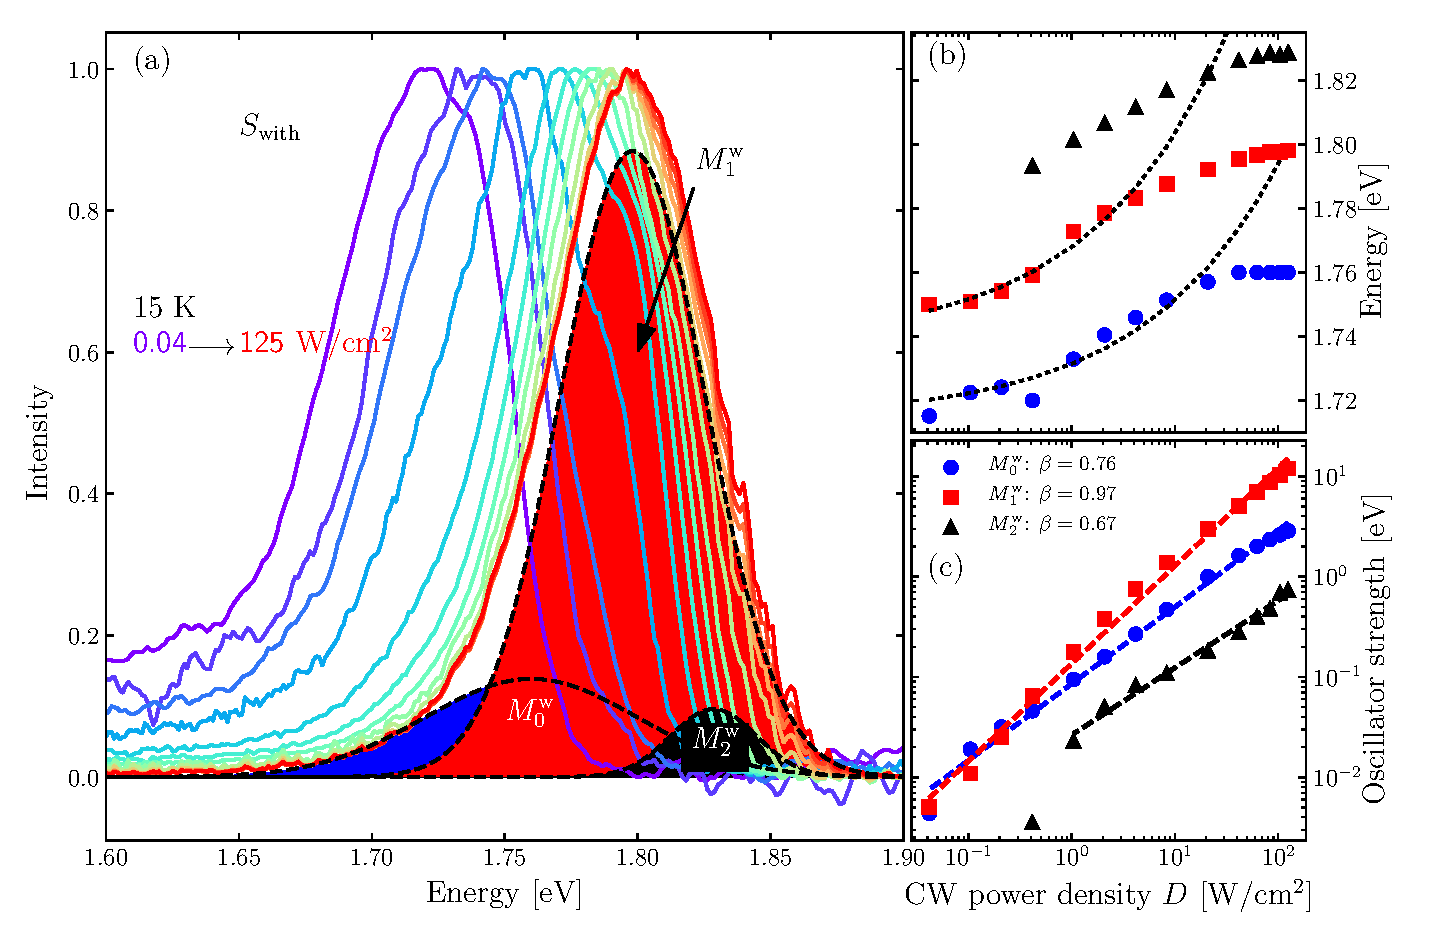
\includegraphics[width=0.9\linewidth]{/PL/intensity/12040_1113_norm_PL_int}
	\caption{(a) PL spectra of $S_\mathrm{with}$ as a function of excitation density were measured from 0.04 to 125~W/cm$^2$ and deconvolved by three Gaussian profiles ($M_0^\mathrm{w}$ blue, $M_1^\mathrm{w}$ red and $M_2^\mathrm{w}$ black shaded area). Fitted parameters - energy and oscillator strength are depicted in panels (b) and (c), respectively. Energies are fitted by Eg.~\ref{eq:PL_intmodel} (dotted curves in (b)), oscillator strengths by linear curve (dashed lines in (c)).}
	\label{fig:QD_w_int}
\end{figure}

Three Gaussian profiles ($M_0^\mathrm{w}$, $M_1^\mathrm{w}$ and $M_2^\mathrm{w}$) in PL spectra were fitted and studied as a function of excitation density $D$ in the range between 0.04 and 125~W/cm$^2$, see Fig.~\ref{fig:QD_w_int}. In Fig.~\ref{fig:QD_w_int}(b) and (c) we show the emission energy and oscillator strength of individual bands as a function of $D$, respectively. The energies of $M_0^\mathrm{w}$ and $M_1^\mathrm{w}$ are fitted by Eq.~\ref{eq:PL_intmodel}, but we can see the third root behaviour only in the beginning of the dependence, then the energies start to be saturated. The whole evolution of energy versus pumping power is much better characterized using the self-consistent multi-particle calculations as in Ref.~\citep{Klenovsky2017}.

The dependencies for oscillator strengths were fairly well fitted by the linear function in the whole range.




\subsubsection*{Sample with capped QDs $\mathbf{S_\mathrm{cap}}$}
\begin{figure}
	\centering
	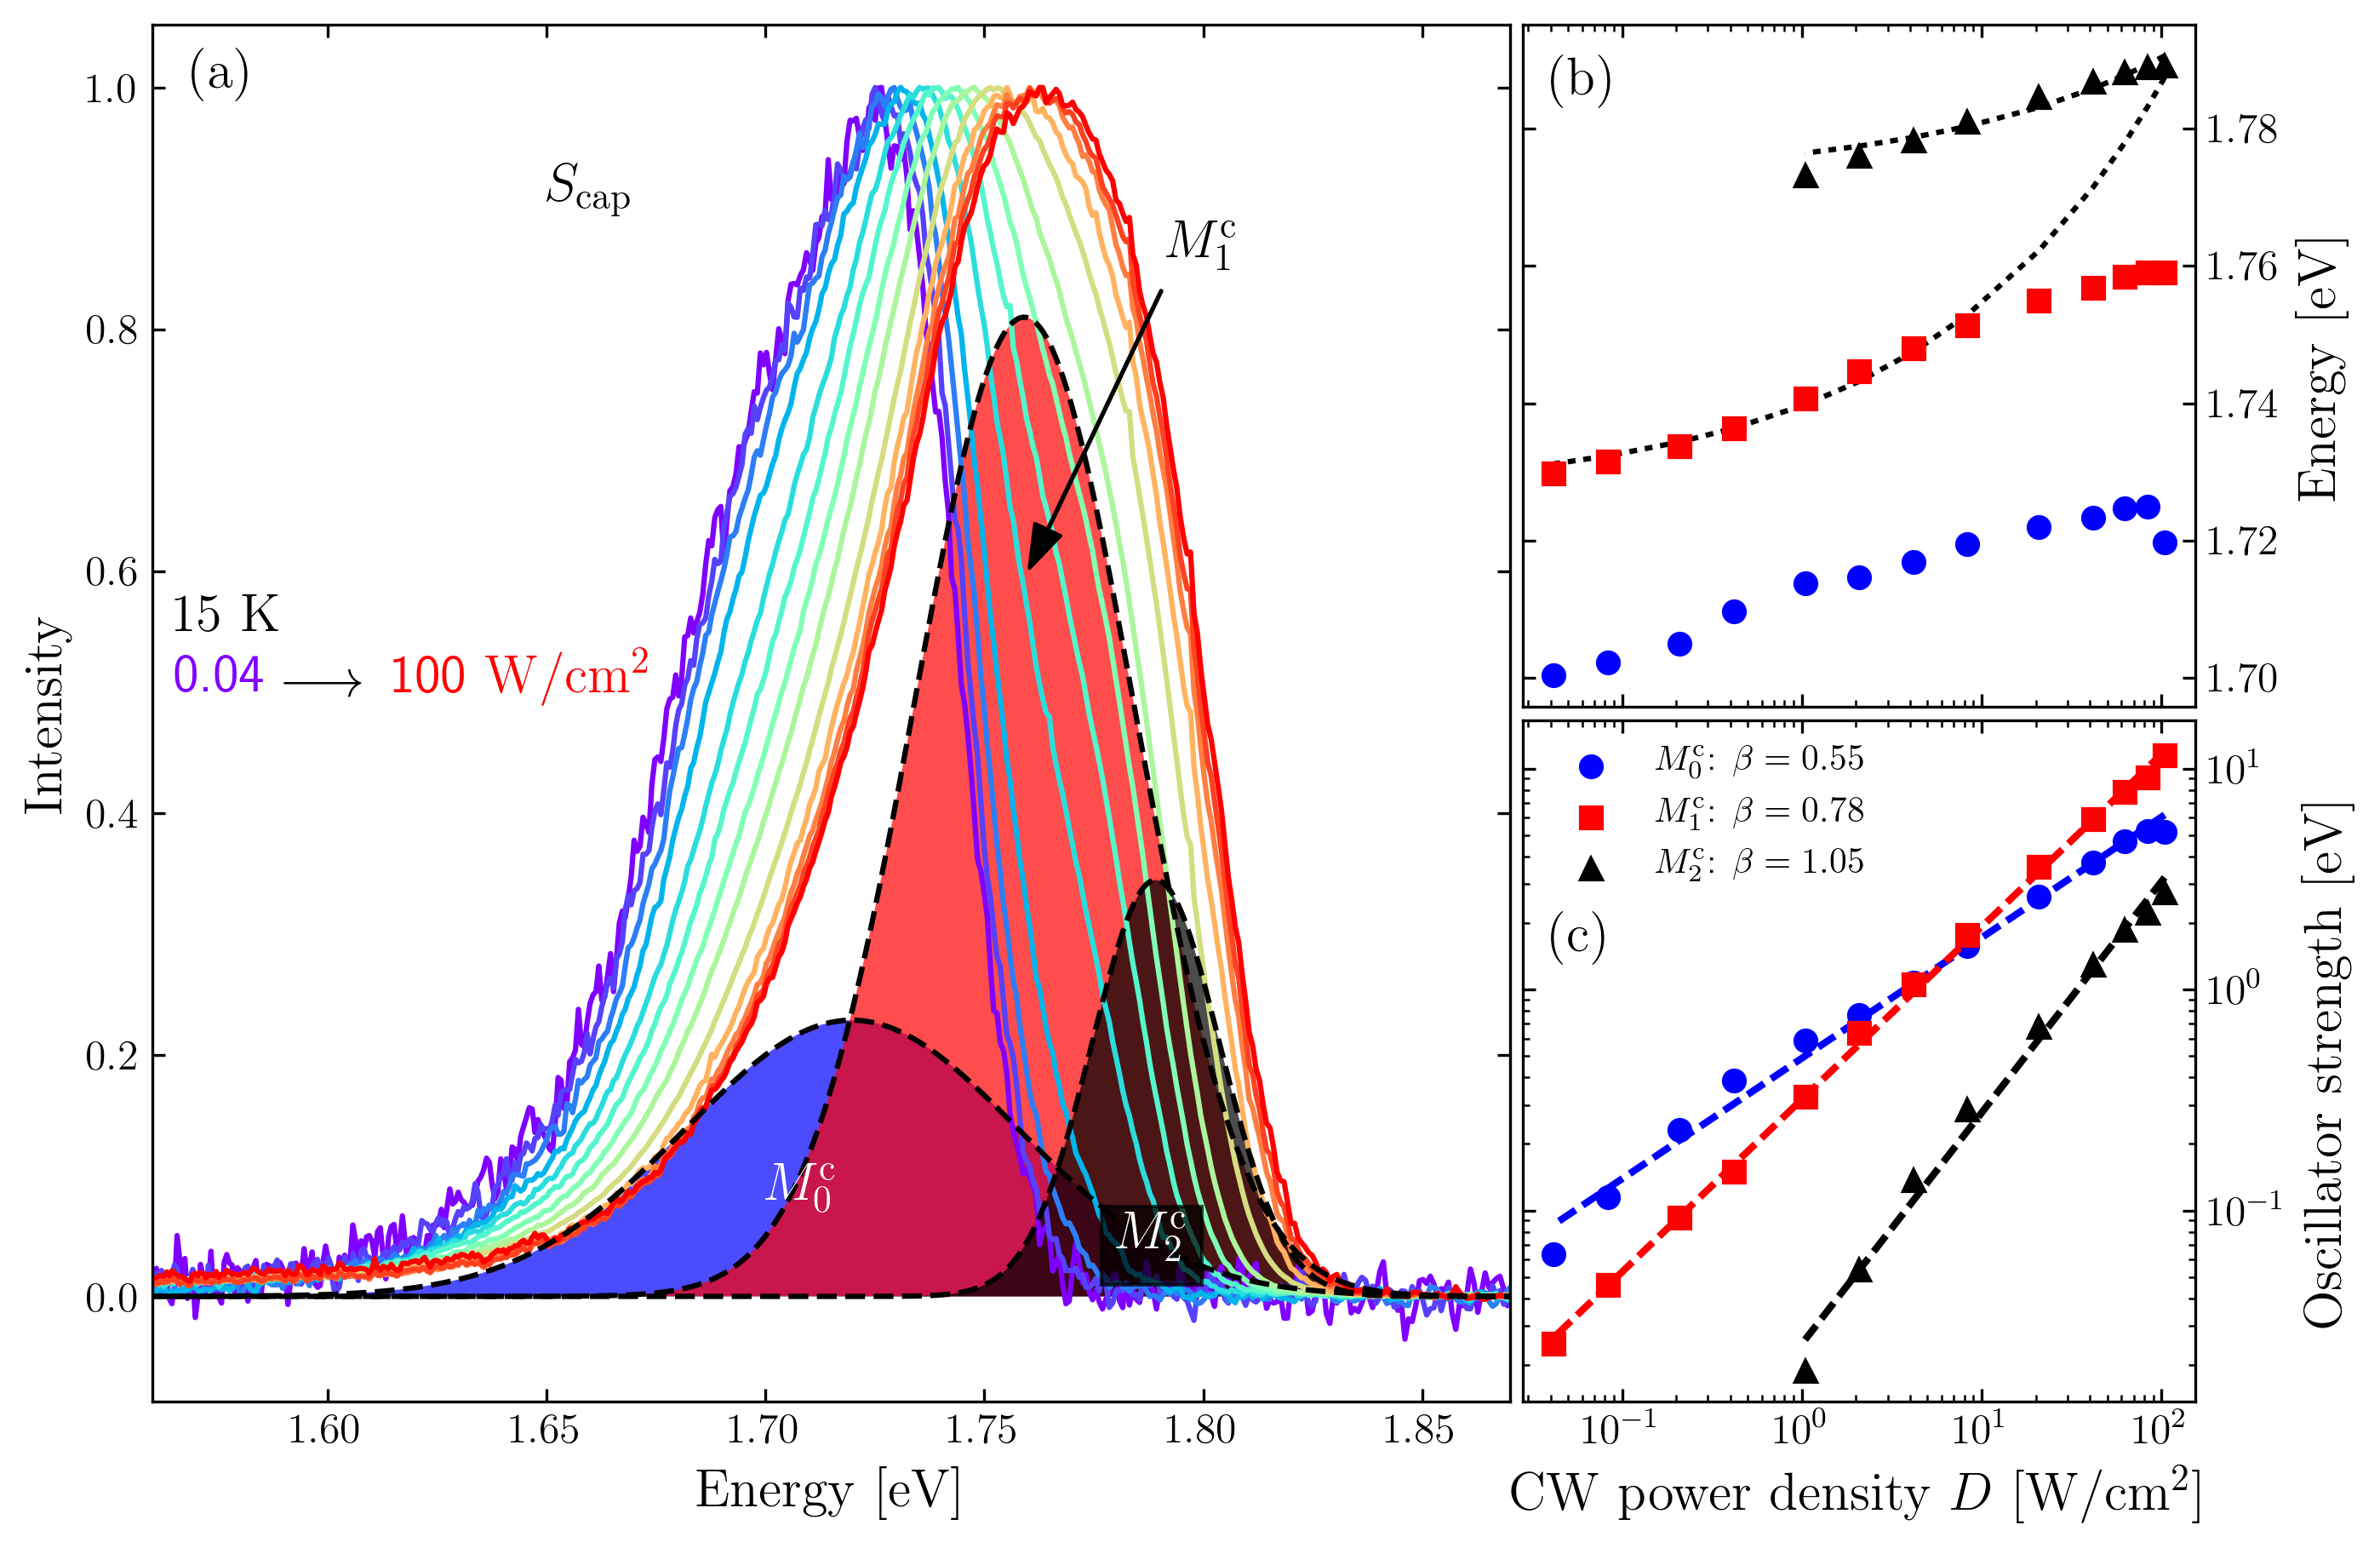
\includegraphics[width=0.9\linewidth]{/PL/intensity/12021_1108_norm_PL_int}
	\caption{The results are given in the same nomenclature as in Fig.~\ref{fig:QD_w_int}.}
	\label{fig:QD_cap_int}
\end{figure}

Intensity-resolved PL spectra of ${S_\mathrm{cap}}$ were treated similarly as for sample ${S_\mathrm{with}}$ and can be seen in Fig.~\ref{fig:QD_cap_int}. All fitted parameters are summarized in Tab.~\ref{tab:int_params}.
\begin{table}
	\centering
	\caption{Summary of the fitting parameters of power density dependent PL for all samples.}
	\begin{tabularx}{0.75\textwidth}{cCCc}
		\toprule
		
		transition & $E_\mathrm{I}$ [meV]& $\gamma$ [$10^{-5}$]& $\beta$ [$\mathrm{W^{2/3}cm^{2/3}s^{-2/3}}$]\\ 	
		\midrule
		\midrule
		$M_0^\mathrm{w/o}$& $1819\pm1$ & $-5\pm6$& $0.55\pm0.02$\\
		$M_1^\mathrm{w/o}$& $1830\pm1$ & $114\pm9$& $0.79\pm0.02$\\
		$M_2^\mathrm{w/o}$ & $1858\pm1$ & $148\pm9$& $0.66\pm0.03$\\ 
		
		\midrule
		$M_0^\mathrm{w}$& $1714\pm3$ & $1700\pm200$& $0.76\pm0.06$\\
		$M_1^\mathrm{w}$& $1737\pm3$ & $3100\pm300$& $0.97\pm0.02$\\
		$M_2^\mathrm{w}$ & -& -& $0.67\pm0.03$\\ 
		
		\midrule
		$M_0^\mathrm{c}$& - & -& $0.54\pm0.02$\\
		$M_1^\mathrm{c}$& $1727\pm1$ & $1290\pm80$& $0.78\pm0.01$\\
		$M_2^\mathrm{c}$ & $1772\pm1$ & $380\pm30$& $1.05\pm0.04$\\
		
		\bottomrule
	\end{tabularx}\label{tab:int_params}
\end{table}

The evolution of the emission bands of sample $S_\mathrm{cap}$ with excitation intensity is compared with predictions obtained within the semi-self-consistent CI (SSCCI) presented in Ref.~\citep{Klenovsky2017} %and described in chapter~\ref{chap:SciRep} 
for 2.5~nm height In$_{0.15}$Ga$_{0.85}$As$_{0.85}$Sb$_{0.15}$/GaAs/GaP QD by the supervisor. The band $M_1^\mathrm{c}$ is reasonably well reproduced by SSCCI with basis formed from single-particle wavefunctions calculated by $1\times8~\mathbf{k \cdot p}$ method with electrons originating from $L$ and holes form $\Gamma$-point. On the other hand, SSCCI with $8\times8~\mathbf{k \cdot p}$ basis for electrons coming from $\Gamma$-point can desbribe the band $M_2^\mathrm{c}$.
\begin{figure}
	\centering
	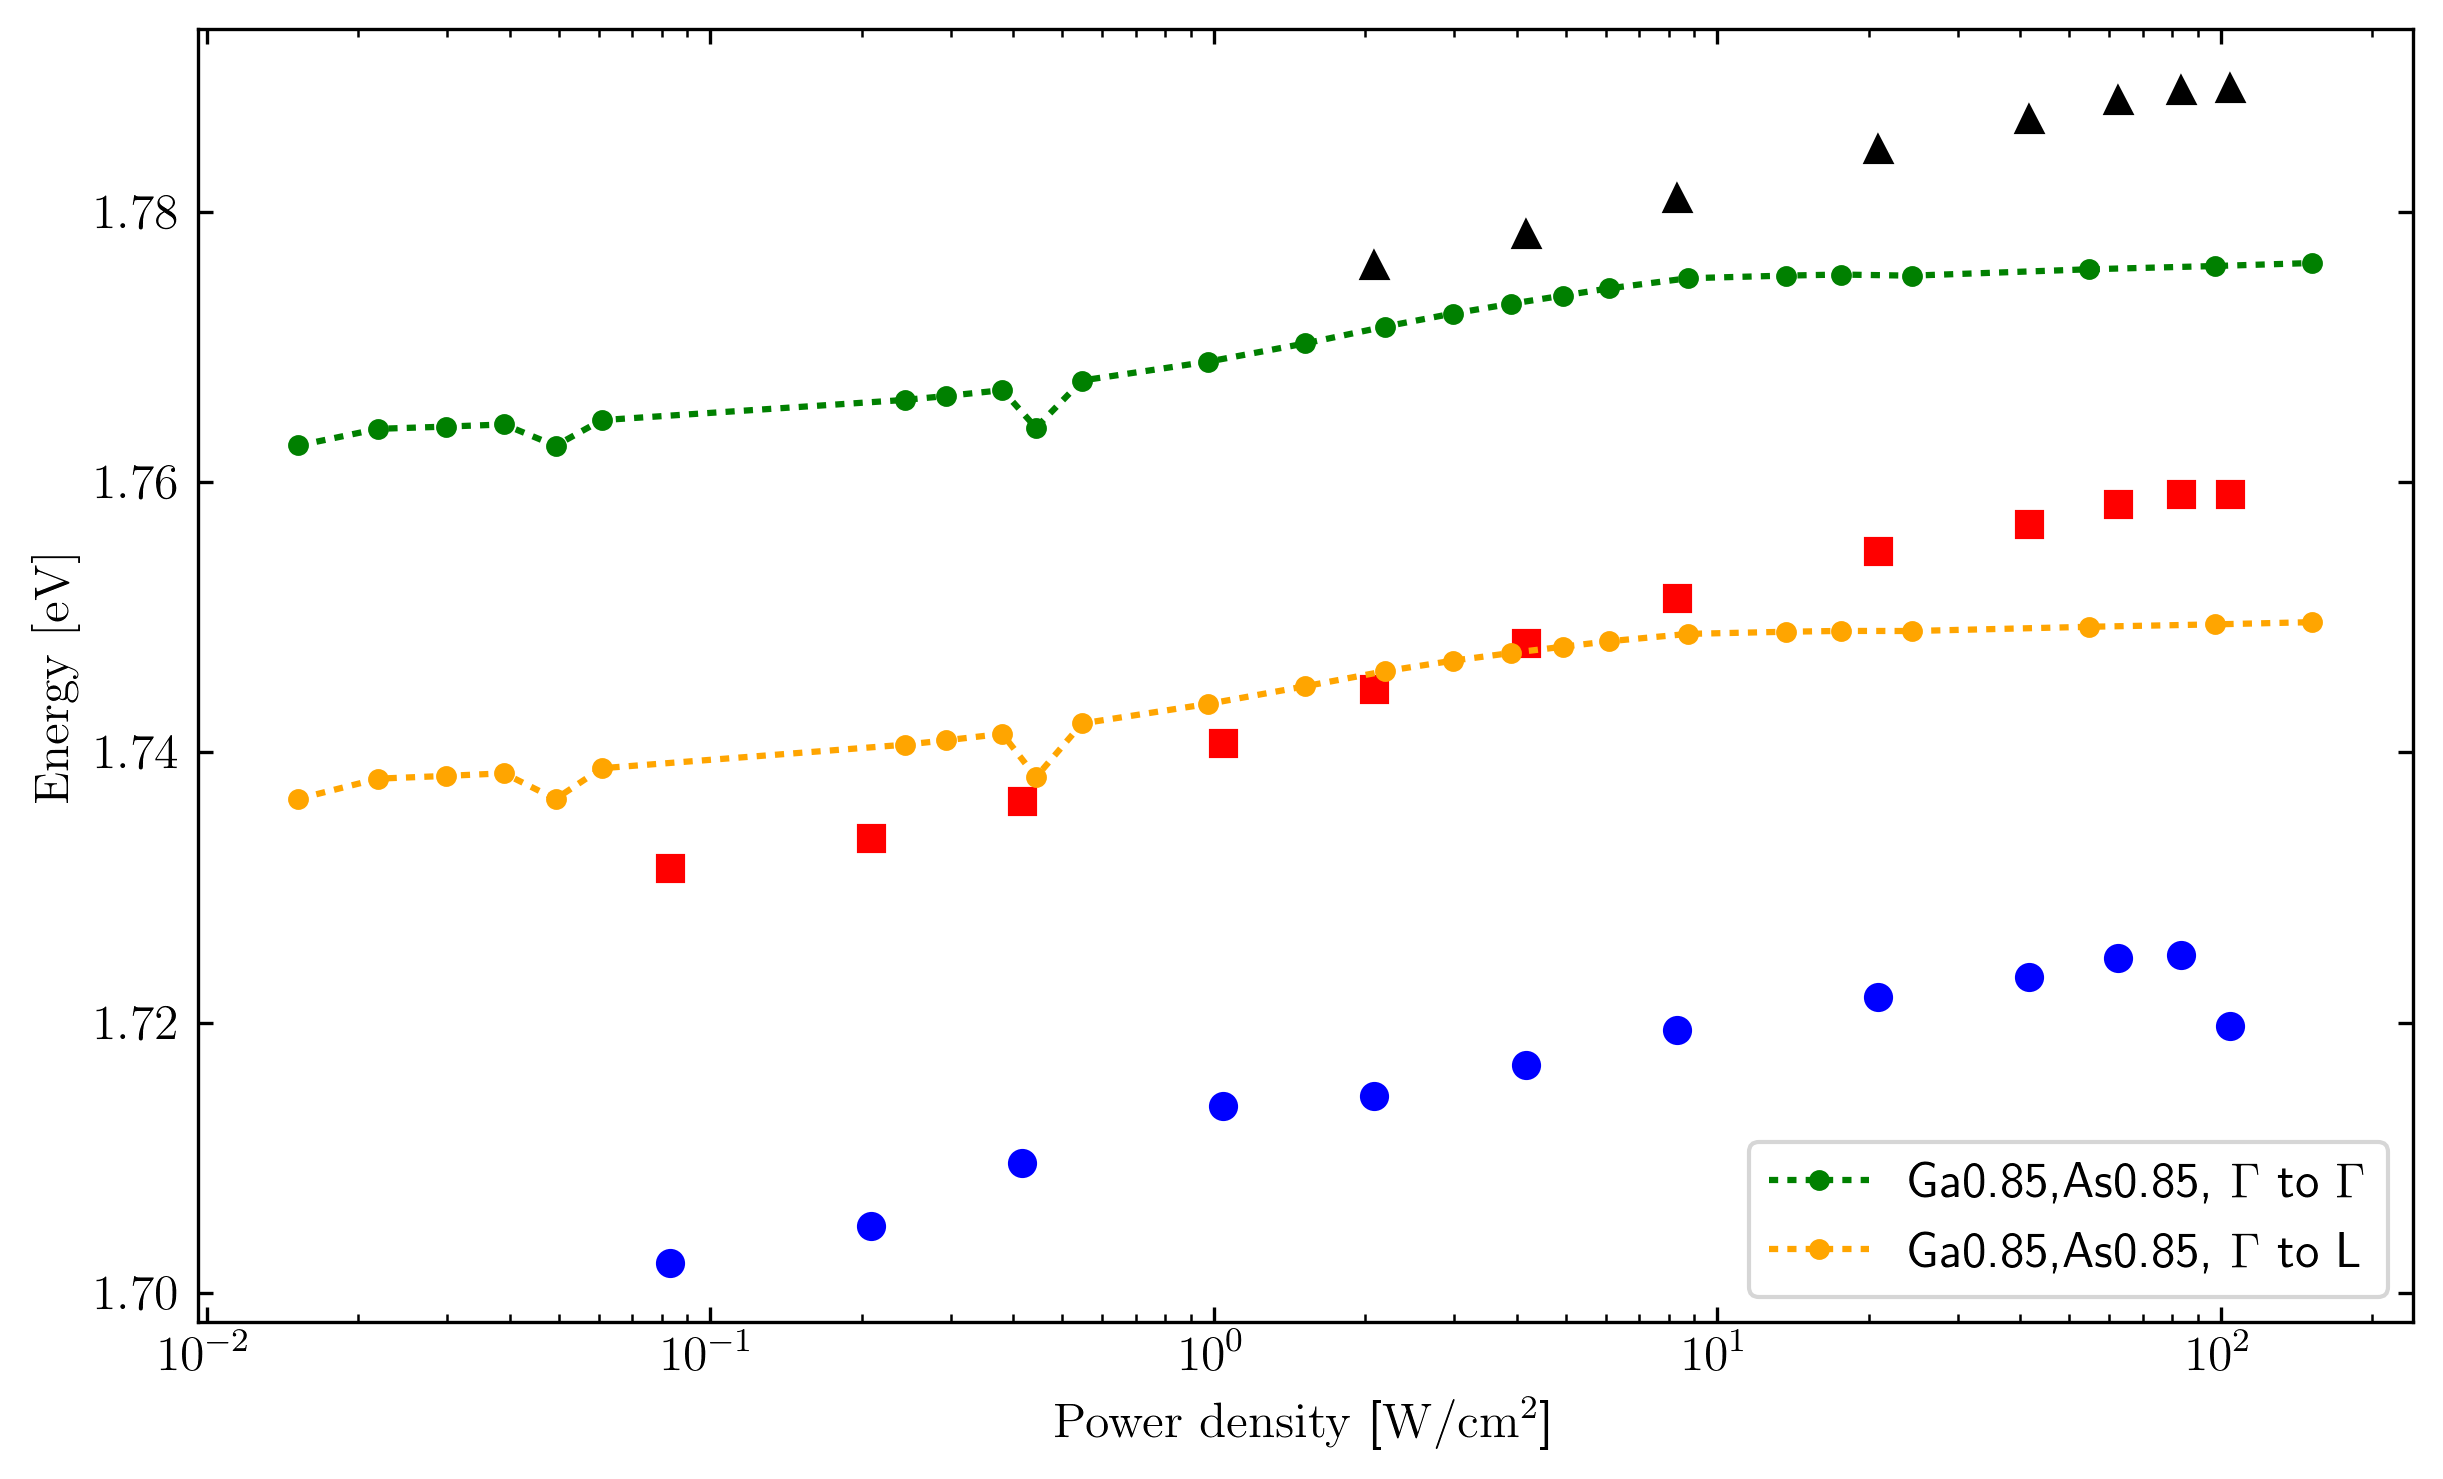
\includegraphics[width=0.9\linewidth]{/PL/intensity/S_cap_expvskpcalc}
	\caption{Emission energy evolution with excitation intensity predicted by SSCCI with single-particle bases calculated by $1\times8~\mathbf{k \cdot p}$ and $8\times8~\mathbf{k \cdot p}$, respectively (dotted curve). To compare experimental points are added.}
	\label{fig:QD_cap_int_expvstheory}
\end{figure}

\newpage
\subsection{Temperature dependent PL}
\label{Sec:temp_PL_TU}
The temperature dependences of the PL of the studied samples was fitted by three Gaussian profiles as in the excitation density investigation in Sec.~\ref{sec:intensity_PL_TU}. The fitted energies were examined using the Varshni-like model
%
\begin{equation}
E(T)=E_0-\frac{\alpha T^2}{T+\Theta_\mathrm{D}}-\frac{\sigma^2}{k_\mathrm{B}T}, \label{eq:Varshni-like}
\end{equation}
where $E_0$ is the energy at temperature $T=0~\mathrm{K}$, $\alpha$ and $\Theta_\mathrm{D}$ are the Varshni parameters, $k_\mathrm{B}$ is Boltzmann constant. The model provides the thermally dependent correction of the empirical Varshni model~\citep{Varshni} describing temperature effects to a band gap of an idealized bulk semiconductor. The estimation proposed by Eliseev~\citep{Eliseev_apl2003_PLtemp} to evaluate the correction is used, which assumes the Gaussian-type distribution of energy of the localized states with broadening parameter $\sigma$.

The mechanisms responsible for the temperature quenching of PL intensity can be accounted for by a Boltzmann model for excitonic recombination with two characteristic activation energies~\citep{Daly_prb1995, Alen_apl2011}
\begin{equation}
I_\mathrm{PL}(T)=\frac{I_0}{1+\tau_0\left[\Gamma_1\exp(-E_1/k_\mathrm{B}T)+\Gamma_2\exp(-E_2/k_\mathrm{B}T)\right]},               \label{eq:Arhenius}
\end{equation}
where $I_0$ is the intensity at 0~K, $\tau_0$ temperature-independent radiative recombination time at 15~K, $E_1$ and $E_2$ are the activation energies of the two quenching mechanisms with related scattering rates $\Gamma_1$ and $\Gamma_2$.%These parameters are representative of the average behaviour of the emissions bands, being the most important $\tau_0$, $E_1$ and $E_2$.
\newpage
\subsubsection*{Sample without QDs $\mathbf{S_\mathrm{w/o}}$}
%
Three recognized emission bands ($M_0^\mathrm{w/o}$, $M_1^\mathrm{w/o}$ and $M_2^\mathrm{w/o}$) in PL of ${S_\mathrm{w/o}}$ are individually investigated from 15~K to 220~K. In this range we can observe Varshni energy-shift of $M_1^\mathrm{w/o}$ and $M_2^\mathrm{w/o}$ described by parameters listed in Tab.~\ref{tab:Varshni}, see Fig.~\ref{fig:QD_wo_temp}(b). In Fig.~\ref{fig:QD_wo_temp}(c) intensity quenching through the temperature range evaluated by the Boltzmann model~(\ref{eq:Arhenius}) is depicted.
%
\begin{figure}
	\centering
	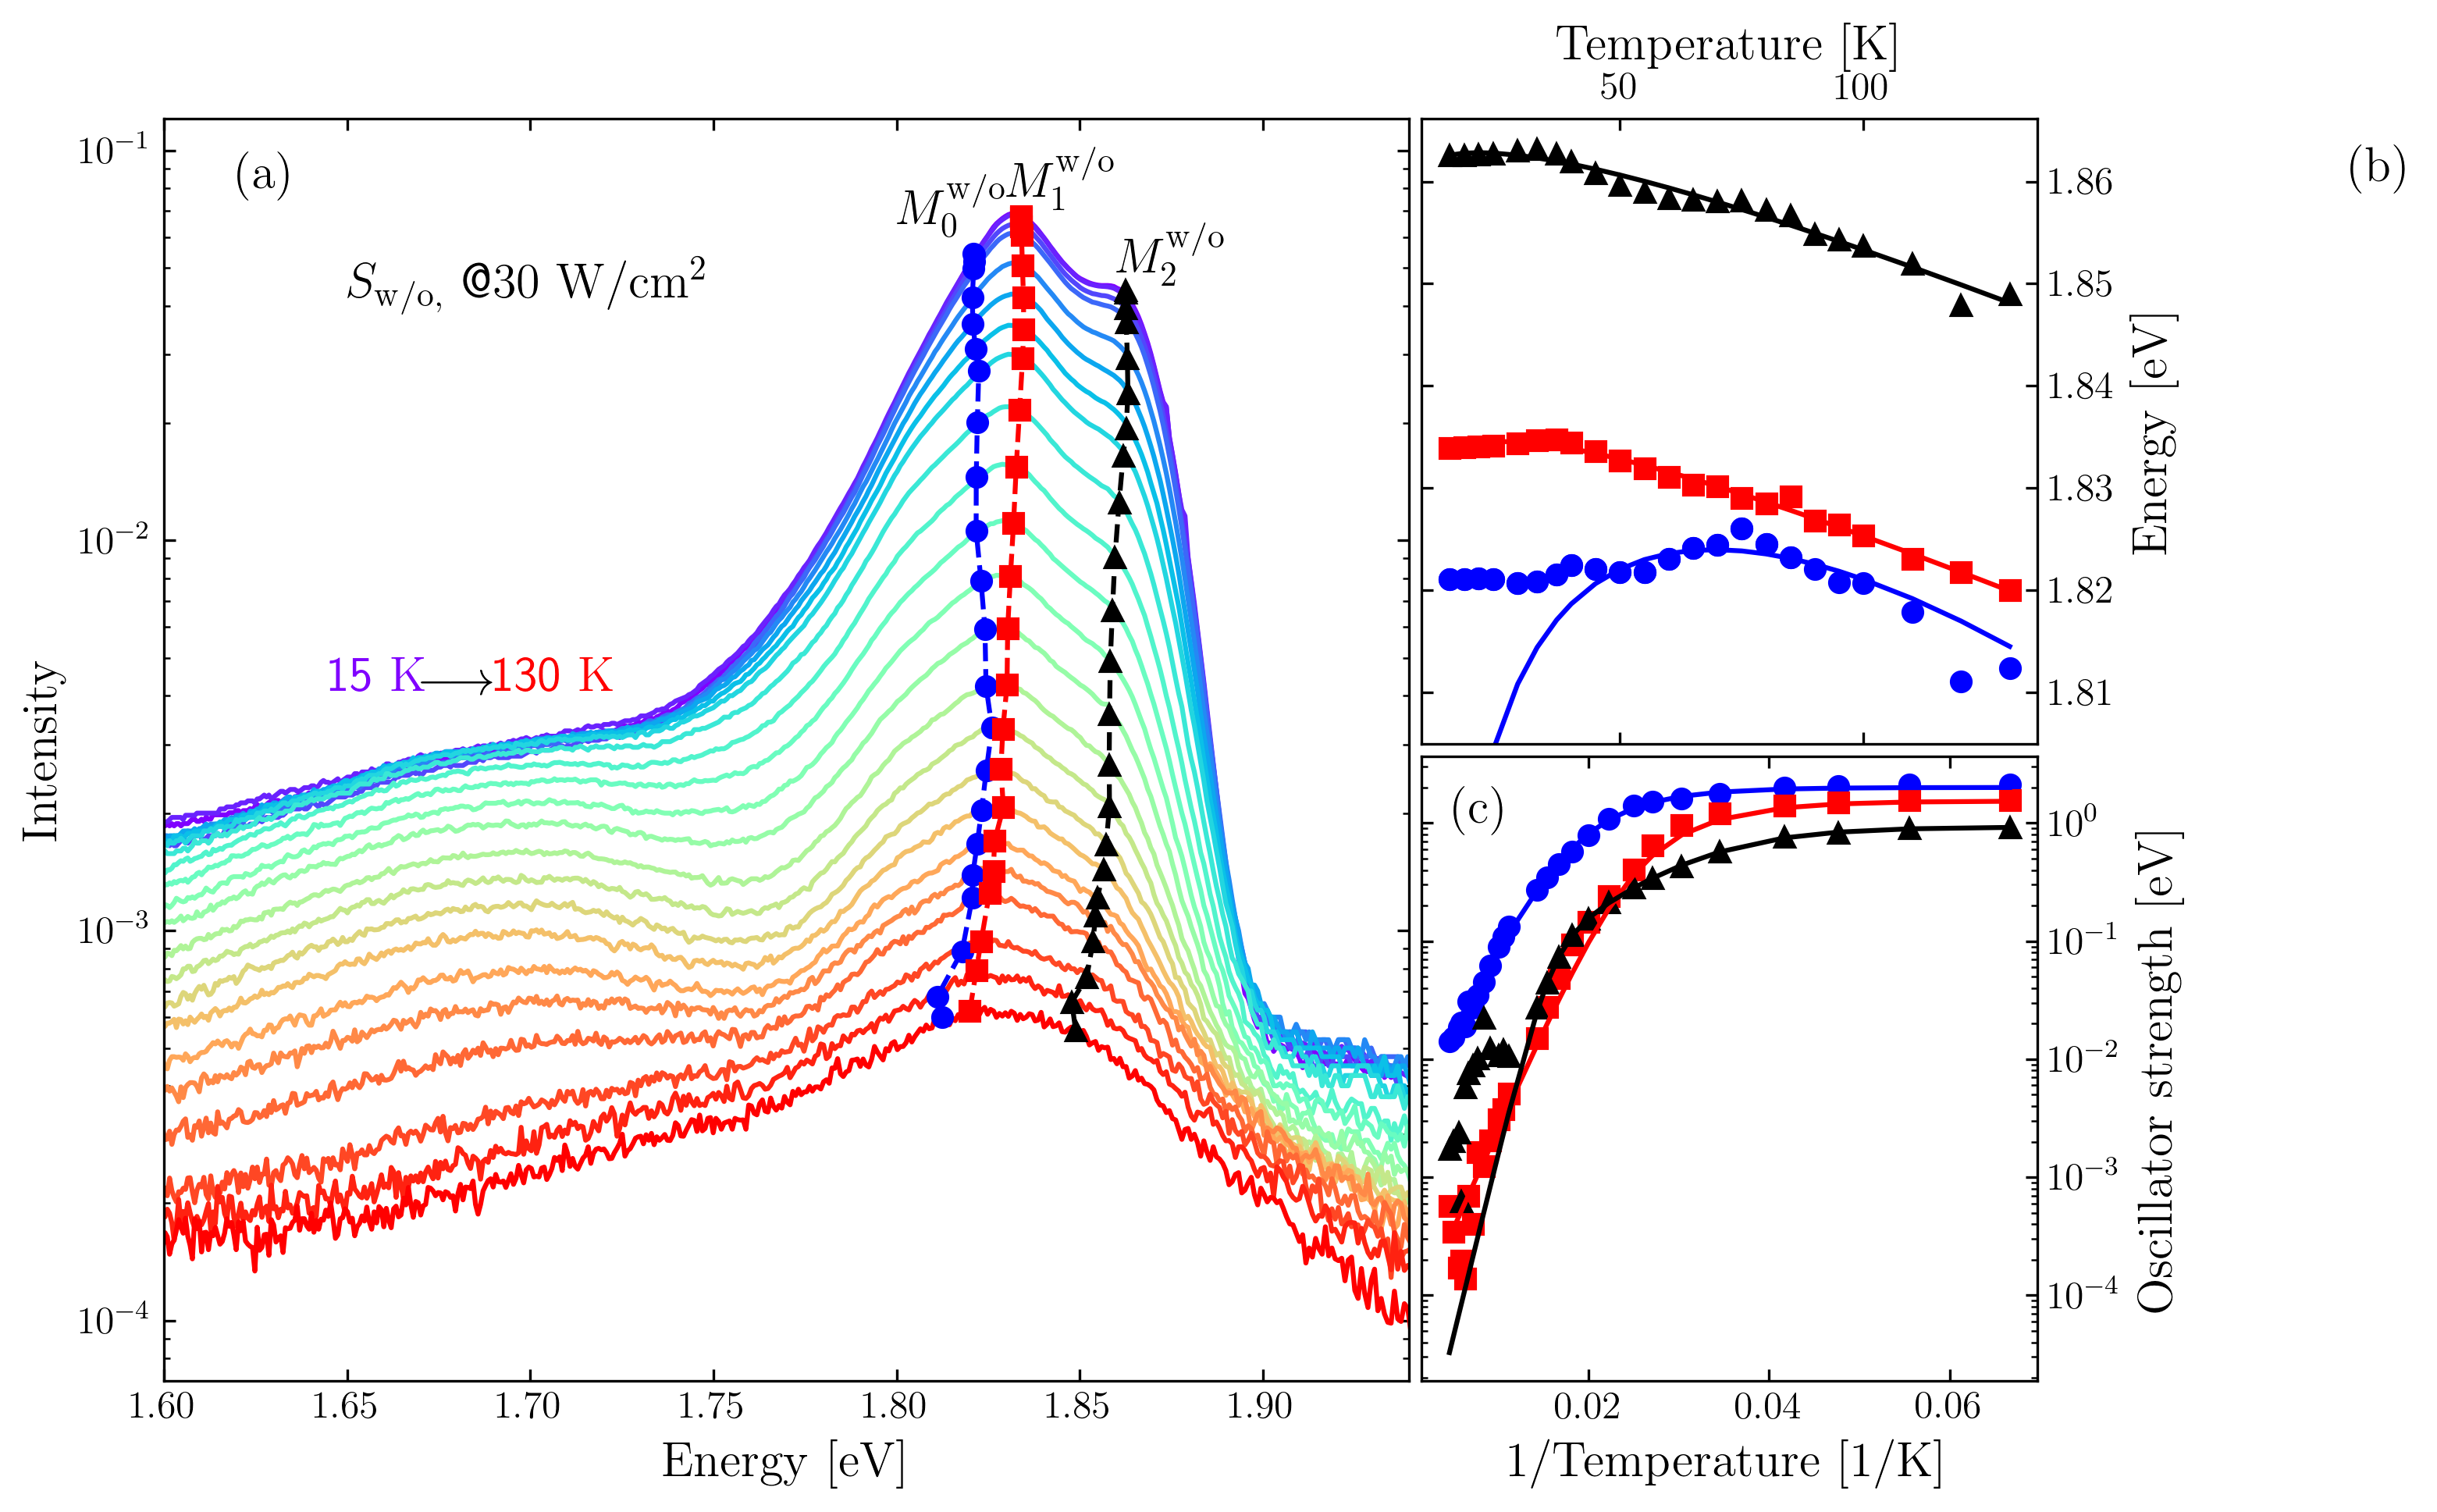
\includegraphics[width=0.9\linewidth]{/PL/temperature/12027_7mW_log_PL_int_without}
	\caption{(a) PL spectra of sample $S_\mathrm{w/o}$ measured at 30~W/cm$^2$ excitation density in 15-220~K temperature range. Each spectrum is fitted by a sum of three Gaussian profiles represented by symbols in panel (a): $M_0^\mathrm{w/o}$ blue circles, $M_1^\mathrm{w/o}$ red squares and $M_2^\mathrm{w/o}$ black triangles. The bands are similarly marked in panels (b) and (c) where also the experimental transition energies (symbols) and fits by the Varshni model~(\ref{eq:Varshni-like}) (lines), respectively, and the integrated PL intensity (symbols) fitted by the Boltzmann model~Eq.~(\ref{eq:Arhenius}) are presented. All fitting parameters are listed in Tabs.~\ref{tab:Varshni} and~\ref{tab:Arhenius}.}
	\label{fig:QD_wo_temp}
\end{figure}


\subsubsection*{Sample with QDs $\mathbf{S_\mathrm{with}}$}
%
In temperature range between 15 and 150~K we observe quenching of PL intensity of three optical transitions marked $M_0^\mathrm{w}$, $M_1^\mathrm{w}$ and $M_2^\mathrm{w}$, see Fig.~\ref{fig:QD_w_temp}(a). The transition energies (Fig.~\ref{fig:QD_w_temp}(b)) and the oscillator strengths (Fig.~\ref{fig:QD_w_temp}(c)) are fitted by the Varshni model~Eq.~(\ref{eq:Varshni-like}) and the Boltzmann model~Eq.~(\ref{eq:Arhenius}) in the whole measured temperature range.  
%
\begin{figure}
	\centering
	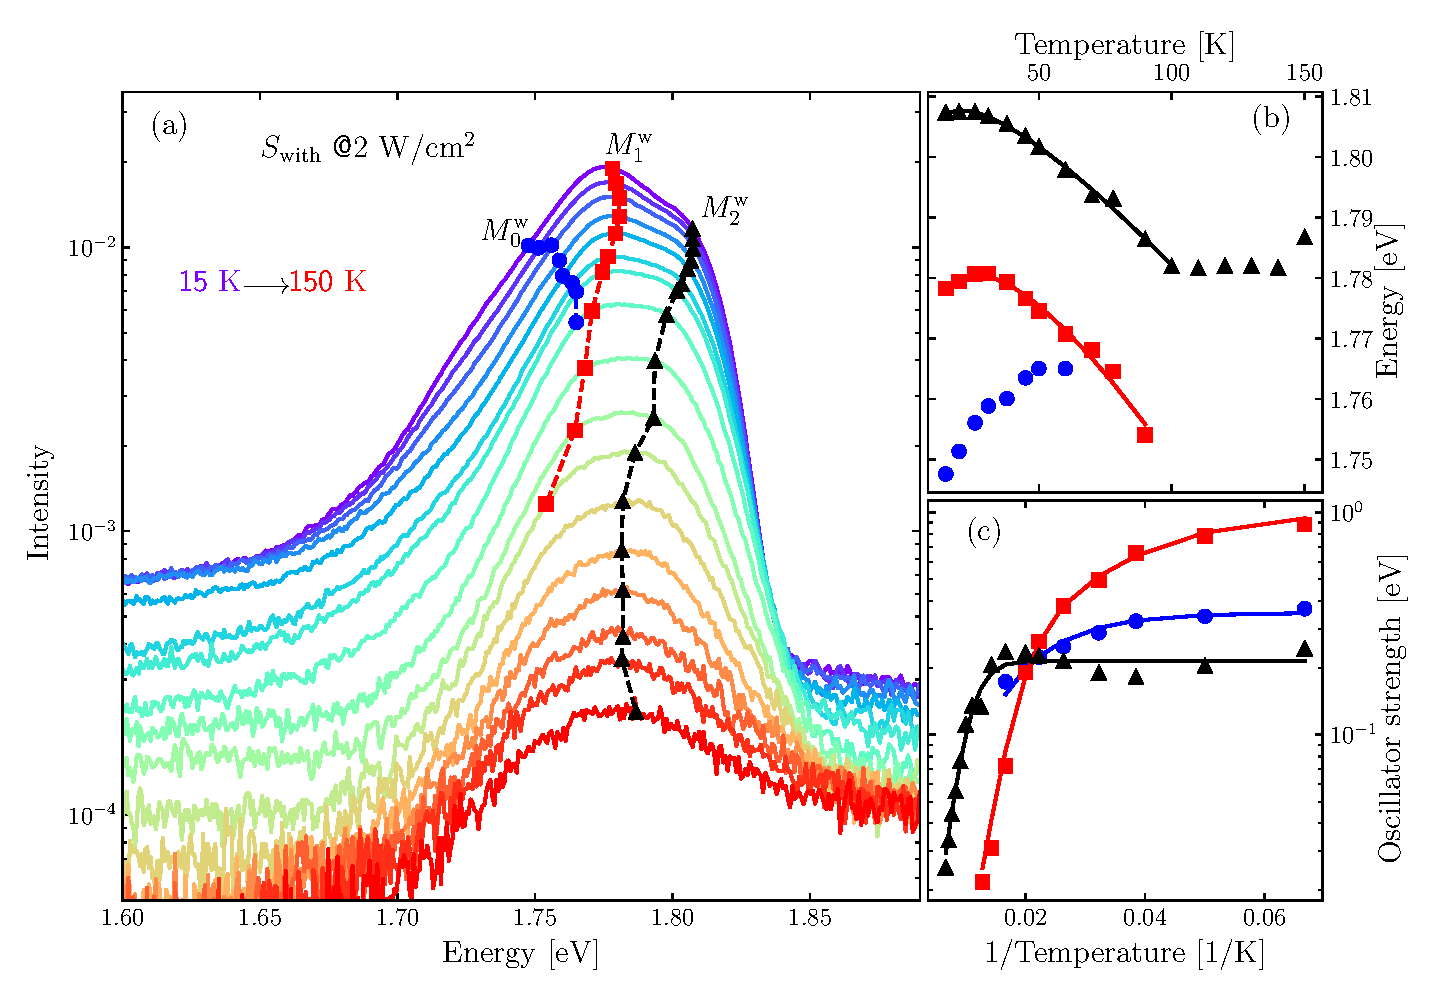
\includegraphics[width=0.9\linewidth]{/PL/temperature/12040_500uW_log_PL_int_Varshni}
	\caption{PL spectra of the sample ${S_\mathrm{with}}$ at 2~W/cm$^2$ between 15 and 150~K. The results are given in the same way as in Fig.~\ref{fig:QD_wo_temp}.}
	\label{fig:QD_w_temp}
\end{figure}

\newpage
\subsubsection*{Sample with capped QDs $\mathbf{S_\mathrm{cap}}$}
%
PL spectra of ${S_\mathrm{cap}}$ are deconvolved into three bands ($M_0^\mathrm{c}$, $M_1^\mathrm{c}$ and $M_2^\mathrm{c}$) and investigated in temperature range 15-110~K, see Fig.~\ref{fig:QD_c_temp}.
%
\begin{figure}[h]
	\centering
	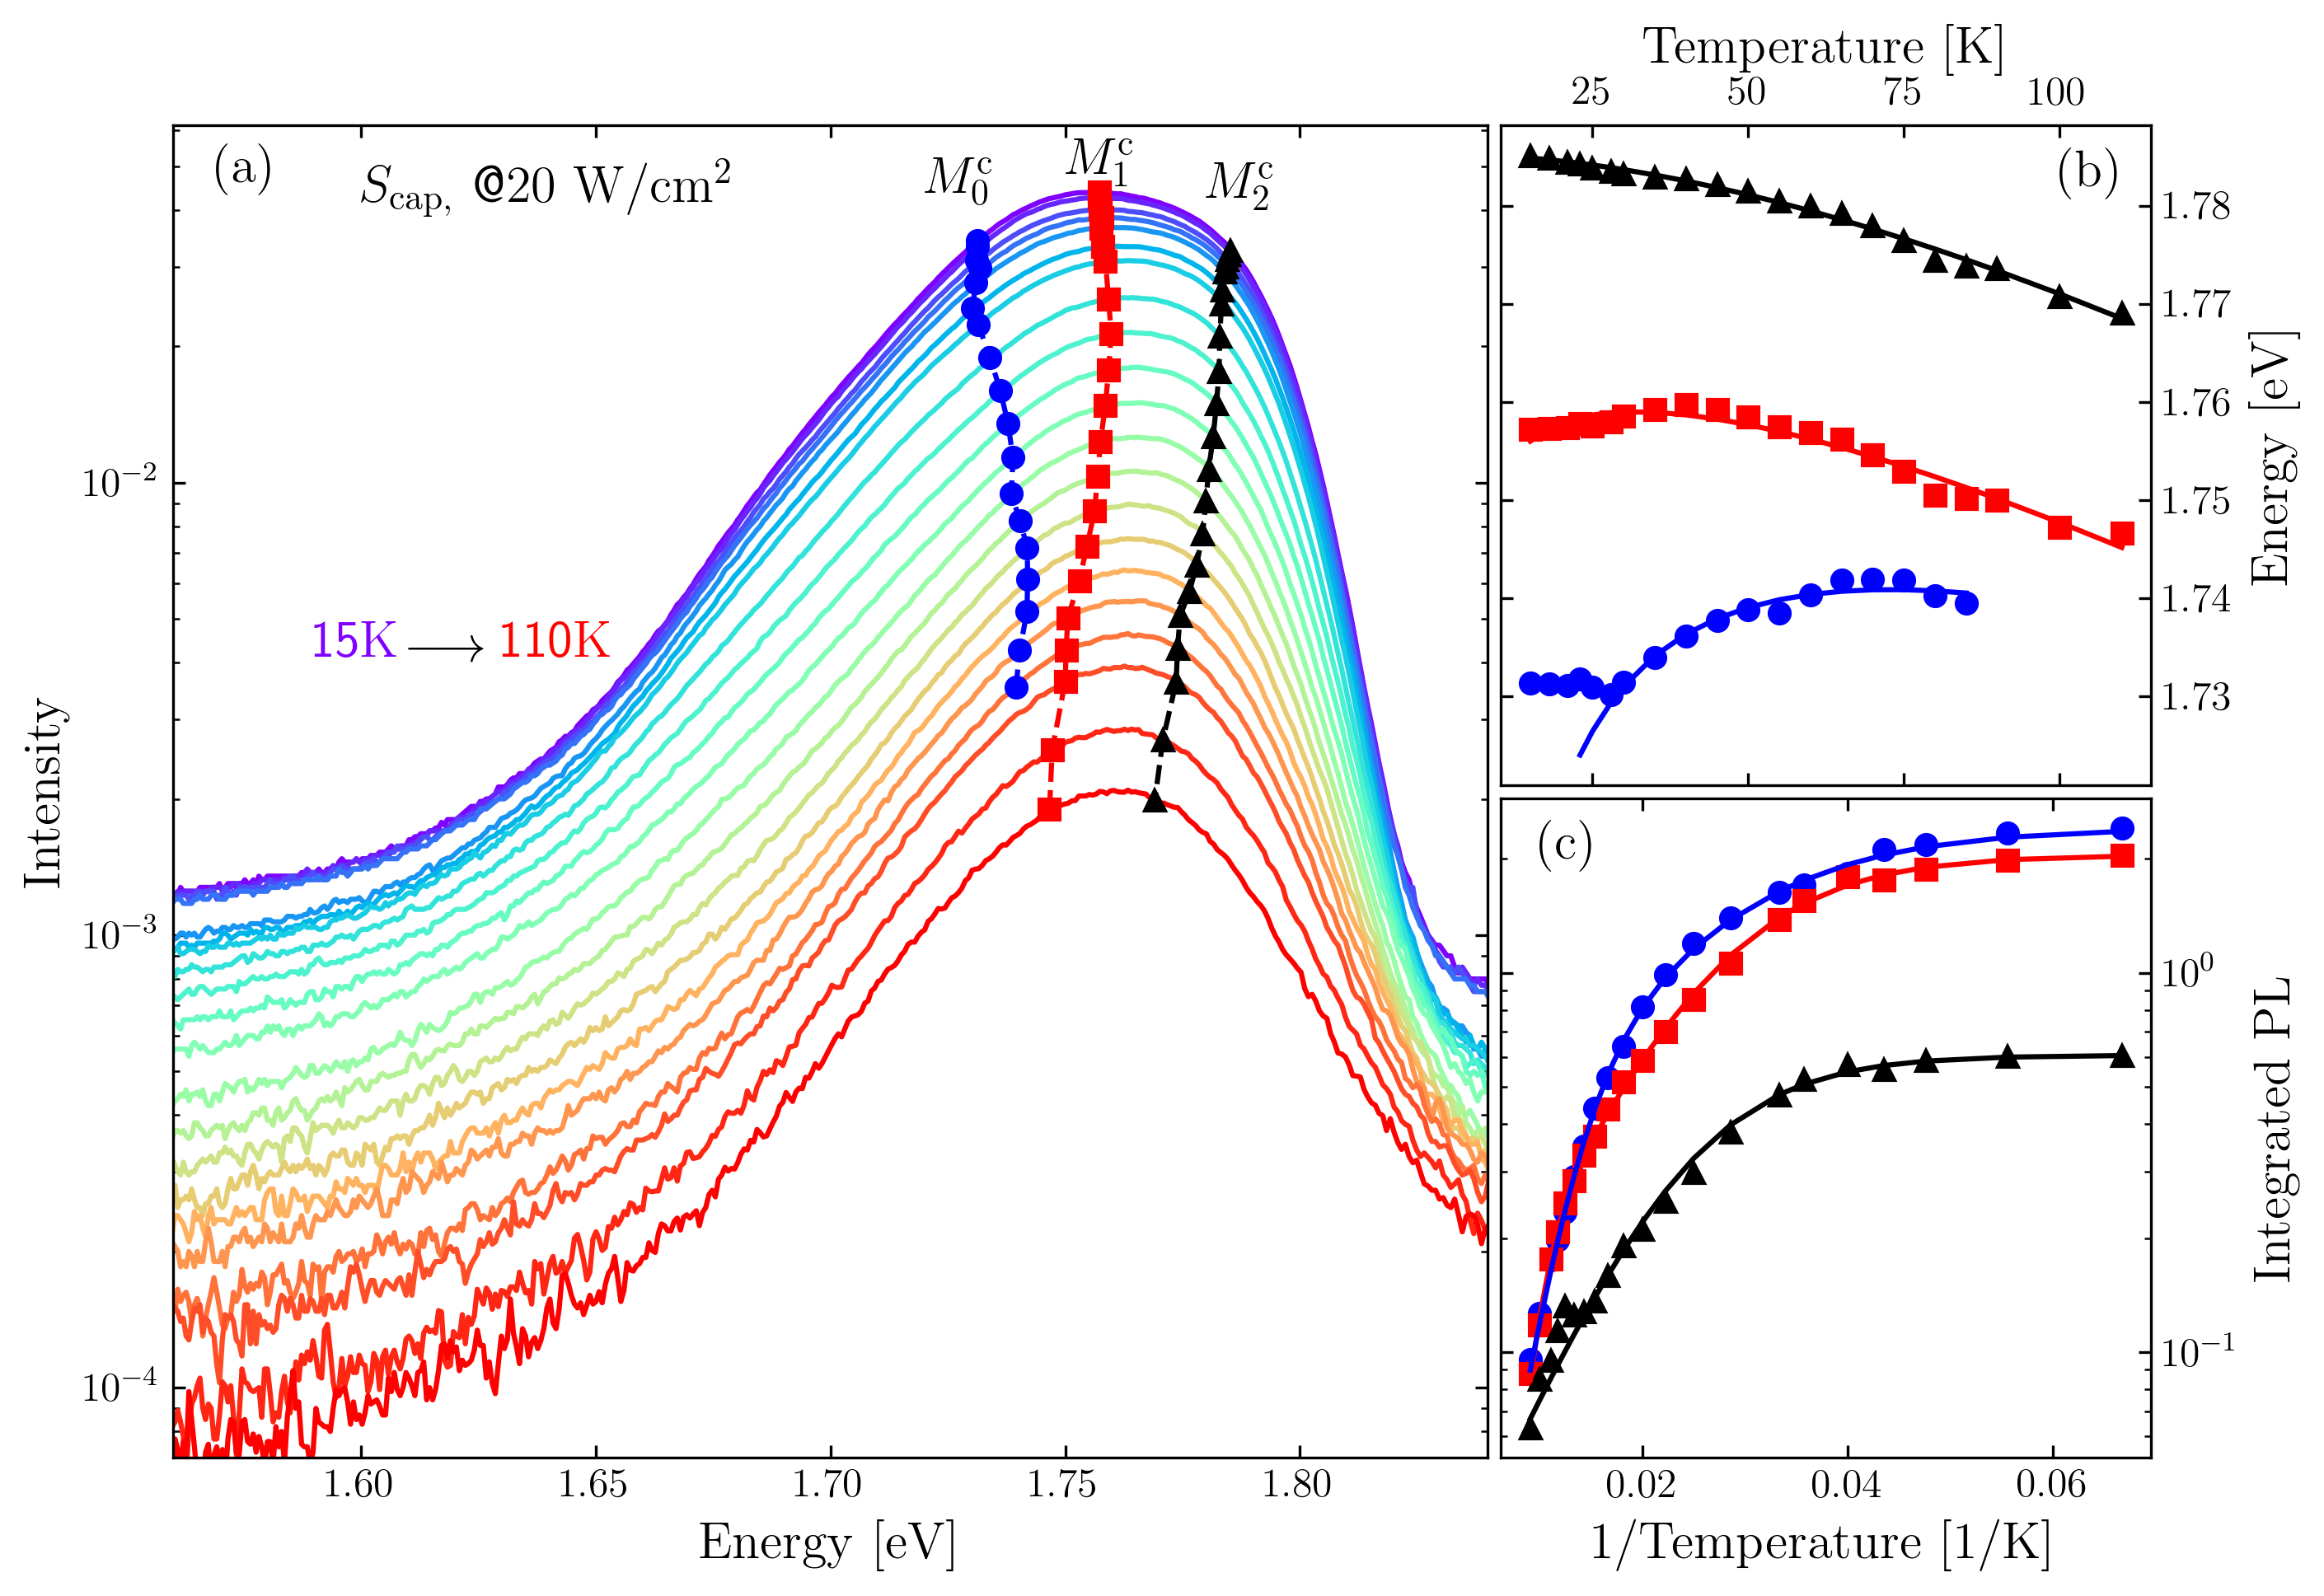
\includegraphics[width=0.9\linewidth]{/PL/temperature/12021_5mW_log_PL_int_Varshni}
	\caption{PL spectra of the sample ${S_\mathrm{cap}}$ measured at 20~W/cm$^2$ between 15 and 110~K. The results are given in the same nomenclature as in Fig.~\ref{fig:QD_wo_temp}.}
	\label{fig:QD_c_temp}
\end{figure}

\newpage
\subsubsection*{Discussion of temperature resolved PL results}
The value of $E_1$ (4--15~meV) is comparable for all samples and also for every PL bands. This low activation energy is determining the low-temperature quenching of the PL and it is usually associated to carrier recombination through impurities. The values of the high-temperature quenching $E_2$ (29--43~meV) are also similar across the samples except the deviation in $M_2^\mathrm{c}$ where we measured extremely small activation energy ($E_2=1$~meV) and $M_2^\mathrm{w/o}$ with $E_2$ twice larger than for other bands ($E_2=62$~meV).

\begin{figure}
	\centering
	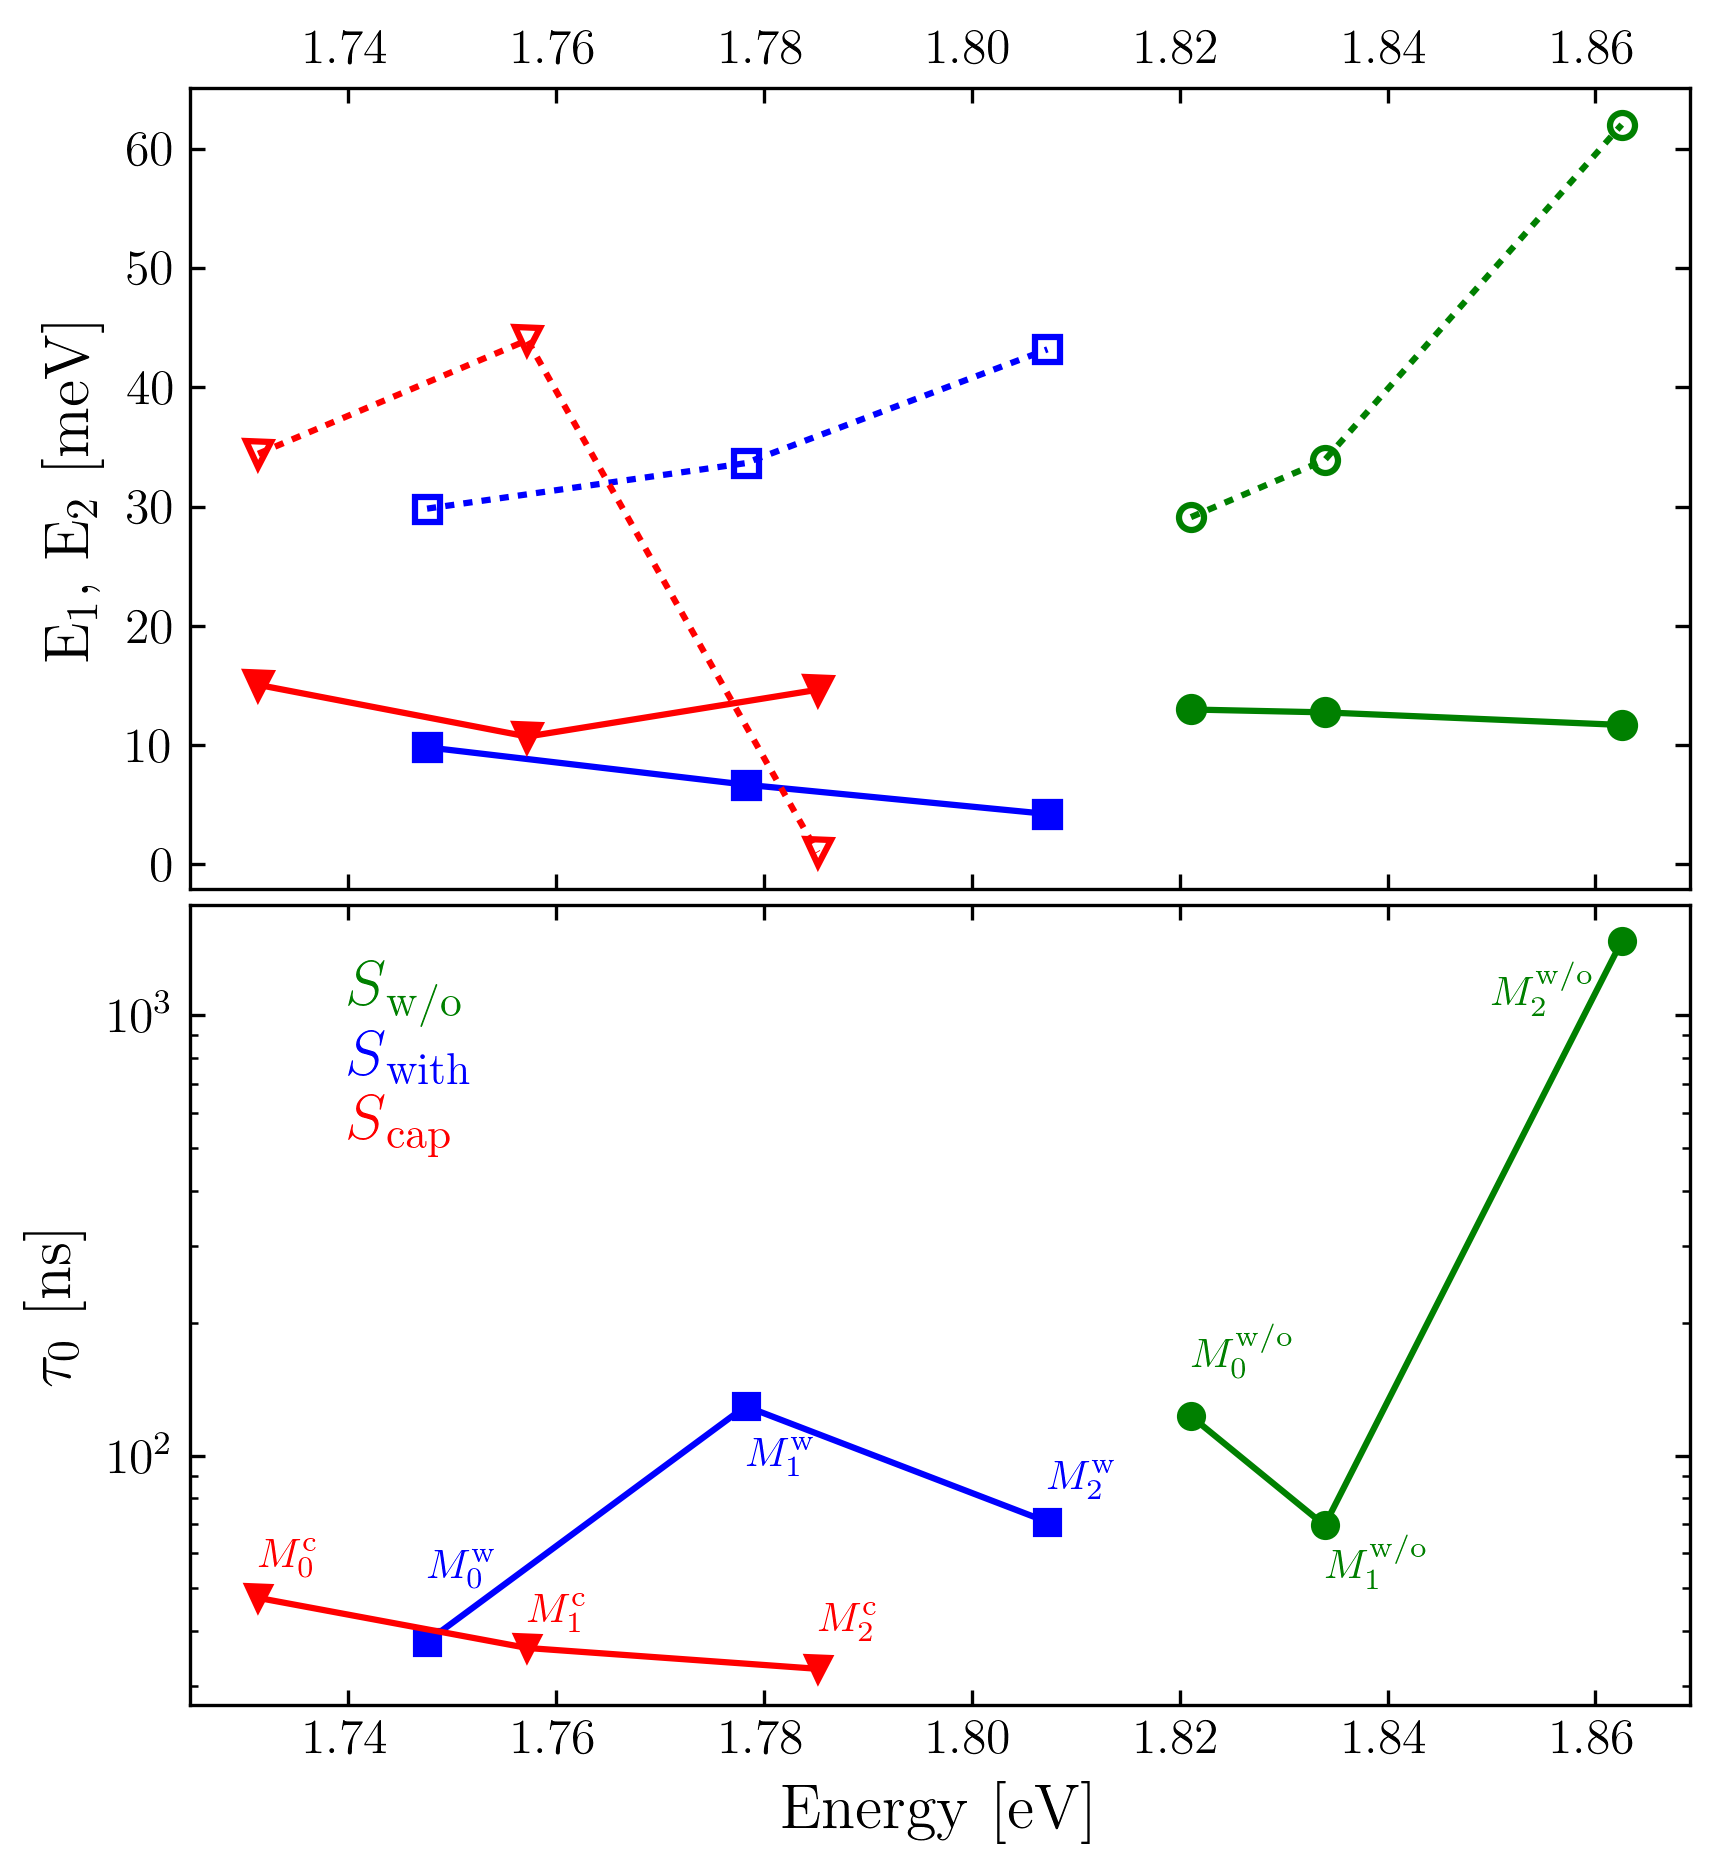
\includegraphics[width=0.75\linewidth]{/PL/temperature/all_Arhenius}
	\caption{Comparison of the Boltzmann fitting parameters for the studied samples. The upper panel depicts $E_1$ (empty symbols) and $E_2$ (full symbols), respectively, the bottom panel shows $\tau_0$. Samples are distinguished by the type and colour of symbols as in Fig.~\ref{fig:PL_homogenity}.}
	\label{fig:Arrhenius_all}
\end{figure}


\begin{table}
	\centering
	\caption{Summary of the Varshni-like fits. The accuracy of $E_0$ and $\alpha$ are better than $10^{-4}\%$, and better than 5~\% for $\Theta_\mathrm{D}$ and $\sigma$.}
	\begin{tabularx}{0.9\textwidth}{cCCcc}
		\toprule
		
		transition & $E_0$ [meV]& $\alpha$ [$10^{-4}~\mathrm{eVK^{-1}}$]& $\Theta_\mathrm{D}$ [K]& $\sigma$ [meV]\\ 	
		\midrule
		\midrule
		$M_0^\mathrm{w/o}$& - & -& -&-\\
		$M_1^\mathrm{w/o}$& $1841$ & $1.69$& $11.2$&$2.6$\\
		$M_2^\mathrm{w/o}$ & $1868$ & $1.61$& $11.6$& $2.5$\\ 
		
		\midrule
		$M_0^\mathrm{w}$& - & -& -&-\\
		$M_1^\mathrm{w}$& $1792$ & $9.99$& $150.1$&$4.0$\\
		$M_2^\mathrm{w}$ & $1815$& $5.49$& $74.5$& $2.8$\\ 
		
		\midrule
		$M_0^\mathrm{c}$& - & -& -&-\\
		$M_1^\mathrm{c}$& $1766$ & $4.03$& $144.5$& $3.4$\\
		$M_2^\mathrm{c}$ & $1785$ & $4.90$& $243.2$& $3.3\cdot 10^{-7}$\\
		
		\bottomrule
	\end{tabularx}\label{tab:Varshni}
\end{table}

\begin{table}
	\centering
	\caption{Summary of the Arhenius-like fits. The displayed values are obtained with accuracy better than $10^{-4}~\%$.}
	\begin{tabularx}{0.9\textwidth}{cCCcccc}
		\toprule
		
		%transition & $I_0$ & $\tau_0$ [ns]& $\Gamma_1$ [ns$^{-1}$]& $E_1$ [meV]& $\Gamma_2$ [ns$^{-1}$]& $E_2$ [meV]\\ 	
	%	\midrule
	%	\midrule
	%	$M_0^\mathrm{w/o}$& 7.65135744e-01&   65.2916823&   566.317577&  7.60337981&8.65963570&   27.3857198 \\
	%	$M_1^\mathrm{w/o}$& 4.38191968e-01&   92.4725944&   1.26183745&   15.1174840&   500.994206&   37.1135443\\
	%	$M_2^\mathrm{w/o}$ & 1.00415726e-11&   95.1667043&   34.0939008&   9.27548824&   96.6322136&   36.5620565\\ 
		
	%	\midrule
	%	$M_0^\mathrm{w}$& 3.53321027e-01&   37.8298857&   17.4314590&  9.81156539&   2.85772107 &  29.8347168\\
	%	$M_1^\mathrm{w}$& 9.99521298e-01 &  129.480243 &  864.188777 &  6.67625574&   39.7837356 &  33.6514094\\
	%	$M_2^\mathrm{w}$ & 2.15529619e-01&   70.7125983&   297.344867 &  4.21713415&   25.0223987 &  43.1983367\\ 
		
	%	\midrule
	%	$M_0^\mathrm{c}$& 2.40563456e+00&  47.5372923&   4.03965001&  34.4371546&   1.38672287&   15.0504481\\
	%	$M_1^\mathrm{c}$& 2.05316367e+00&   36.5787466&   81.4268881&   10.7120315&   19.2461237&  43.9676048\\
	%	$M_2^\mathrm{c}$ & 2.61200307e+00&   32.8025509 &  18.6448452 &  1.00000016&   5.01856897&  14.6371152\\
		
		
			transition & $I_0$ & $\tau_0$ [ns]& $\Gamma_1$ [ns$^{-1}$]& $E_1$ [meV]& $\Gamma_2$ [ns$^{-1}$]& $E_2$ [meV]\\ 	
			\midrule
			\midrule
			$M_0^\mathrm{w/o}$&  2.000 &  122.9&   13.17&  13.0&  4.62&   29.1 \\
			$M_1^\mathrm{w/o}$& 1.533&   69.5&  93.62&   12.7&   424.25&  33.9\\
			$M_2^\mathrm{w/o}$ &  0.925 &  1474.1 &  456.81 &  11.7&   506.20 &  62.1\\ 
			
			\midrule
			$M_0^\mathrm{w}$& 0.353&   37.8&   17.43&  9.8&   2.86 &  29.8\\
			$M_1^\mathrm{w}$& 0.999 &  129.5 &  864.19&  6.7&   39.78 &  33.7\\
			$M_2^\mathrm{w}$ & 0.216&   70.7&   297.34 &  4.2&   25.02&  43.2\\ 
			
			\midrule
			$M_0^\mathrm{c}$& 2.406&  47.5&   1.39&   15.0 &   4.04&  34.4\\
			$M_1^\mathrm{c}$& 2.053&   36.5&   81.43&   10.7&   19.25&  44.0\\
			$M_2^\mathrm{c}$ & 2.612&   32.8&   5.02&  14.6 &  18.65 &  1.0\\
			
		\bottomrule
	\end{tabularx}\label{tab:Arhenius}
\end{table}


\clearpage
\subsection{Polarization dependent PL }
In our experiments, both the excitation and the detected PL radiation propagate perpendicularly to the sample surface; the angle between the crystallographic direction~[110] and the polarization vector is denoted $\theta$. Because low degrees of polarization of the emitted light is expected, we visualize our experimental results in terms of the degree of polarization
%
\begin{equation}
C(\theta)=\frac{I(\theta)-I_\mathrm{min}}{I_\mathrm{max}+I_\mathrm{min}},
\end{equation}
%
where $I_\mathrm{min}$ and $I_\mathrm{max}$ are extremal values of $I(\theta)$. Note that for angle $\theta_\mathrm{max}$, such that $I(\theta_\mathrm{max})=I_\mathrm{max}$, the previous relation gives the maximum obtained degree of polarization $C(\theta_\mathrm{max})=C_\mathrm{max}$ (values in the polar graphs~\ref{fig:PL_pol_all}).

Non-polarized PL of GaAs layer on sample ${S_\mathrm{with}}$ is expected, therefore we are using degree of polarization of $M_1^\mathrm{w/o}$ to re-calibrate degree of polarization of other bands to eliminate the residual polarization of the whole setup. The calibrated $C(\theta)$ of individual bands are plotted in Fig.~\ref{fig:PL_pol_all}. Note that almost no polarization anisotropy is observed on sample ${S_\mathrm{w/o}}$.

The emission radiation of samples containing QDs is polarized along the [110]~crystallographic direction, in agreement with results on type-I InAs/GaAs QDs~\citep{HumPhysE} where the polarization anisotropy of $I(\theta)$ is dictated predominantly by the orientation of the wavefunction of hole states. Based on that noticing the results of Ref.~\citep{Klenovsky2015} we conclude that the studied samples are type-I.

 %The sample ${S_\mathrm{with}}$ has $C_\mathrm{max}$ around 0.04, which is typically observable value on InAs/GaAs QDs, where one-particle wavefunctions are precisely located in the same position in the QD. Sb from GaSb capping on ${S_\mathrm{cap}}$ causes that the wavefunctions move slightly toward each other therefore the polarization anisotropy grows up to almost 0.15.
  The sample ${S_\mathrm{with}}$ has $C_\mathrm{max}$ around 0.04, which is comparable to that for InAs/GaAs QDs where one-particle wavefunctions are located in the same position in the QD. Antimony from GaSb capping in sample ${S_\mathrm{cap}}$ causes that the wavefunctions of electrons and holes are positioned slightly further apart from each other therefore the polarization anisotropy grows up to almost 0.15.
  
\begin{figure}
	\centering
	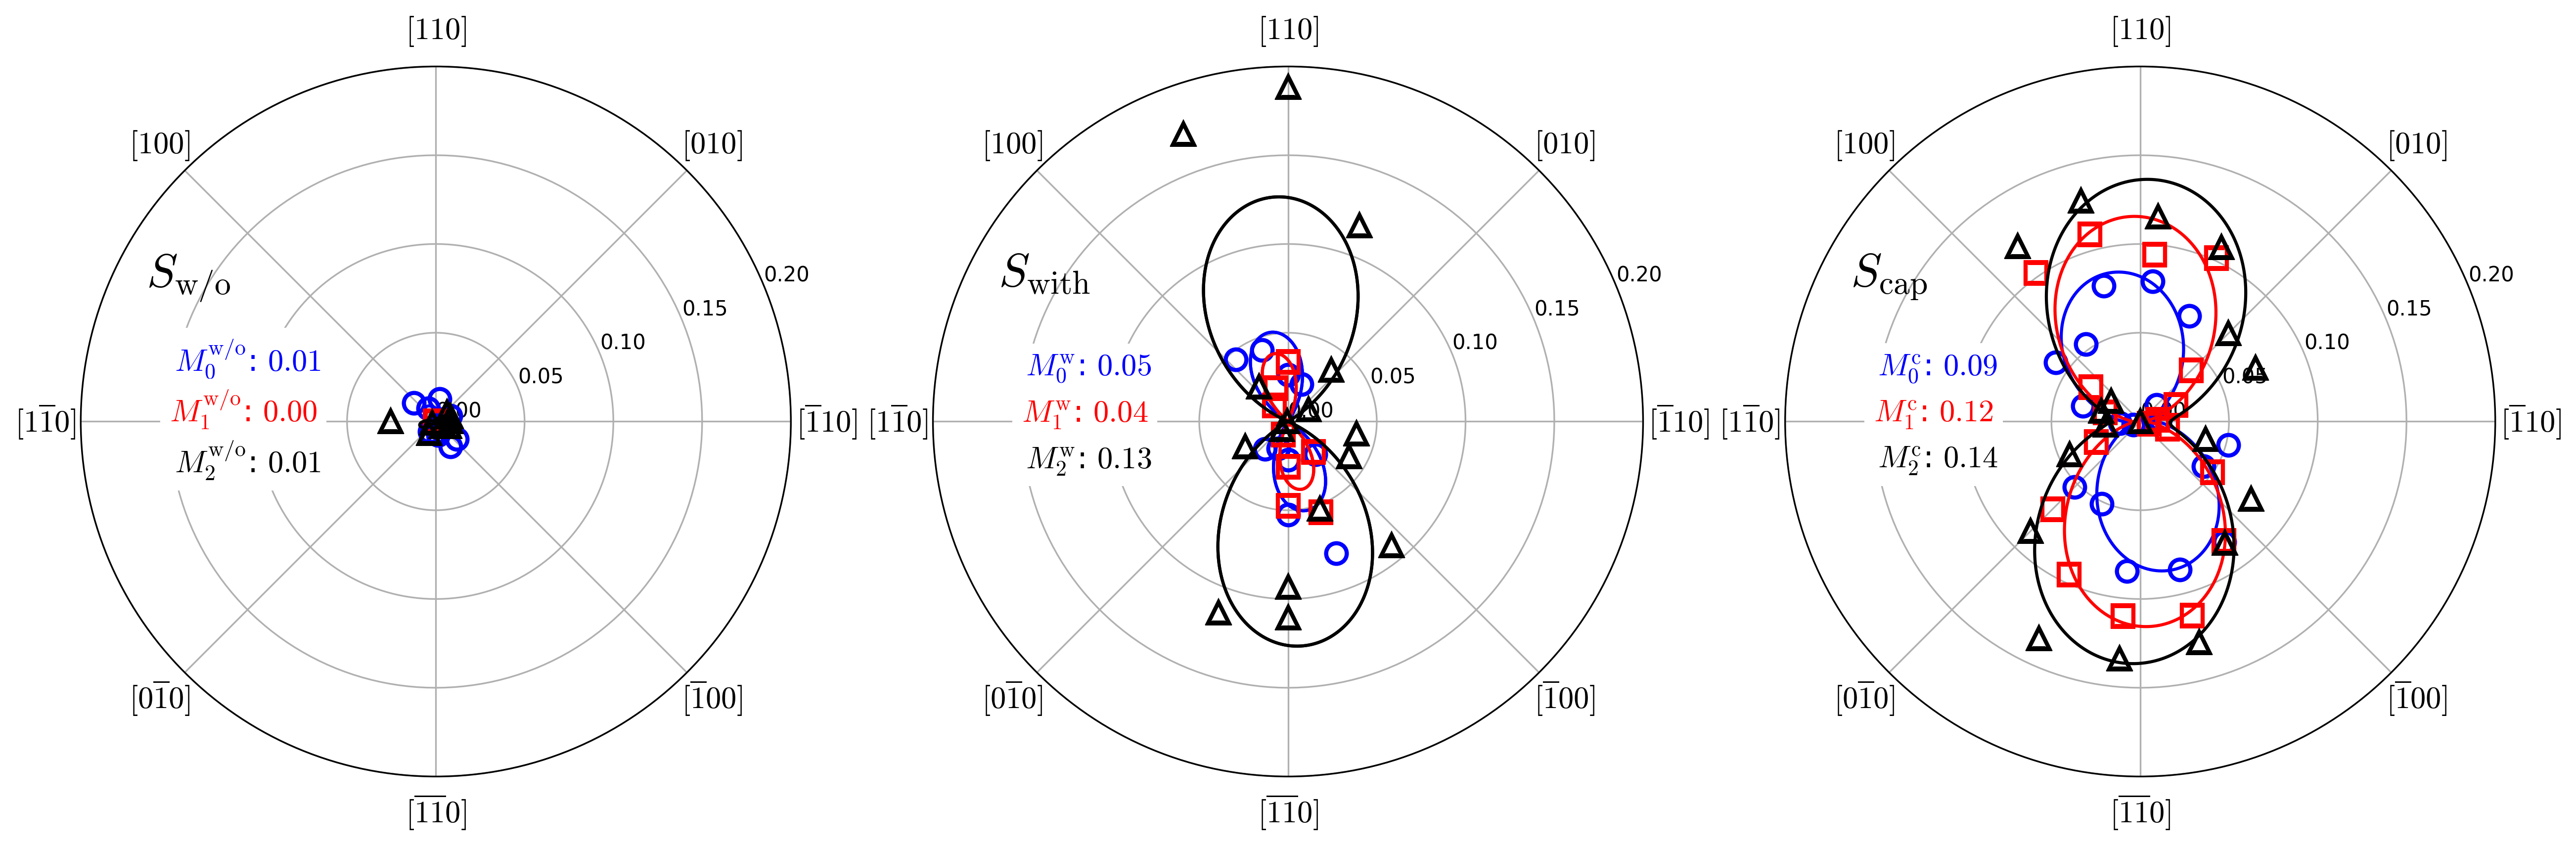
\includegraphics[width=1\linewidth]{/PL/polarization/POL_all}
	\caption{From left to right the polar graphs show $C(\theta)$ of sample ${S_\mathrm{w/o}}$, ${S_\mathrm{with}}$ and $\mathbf{S_\mathrm{cap}}$, respectively. Individual bands of PL spectra for each sample are represented by different symbols, consistently with previous labeling.}
	\label{fig:PL_pol_all}
\end{figure}

\newpage
\section{Time-resolved photoluminiscence}
%The measurements can be fitted to a double exponential decay function after convolution with the instrument response function (IRF) shown in the same graph
We have studied the dynamics of the recombination processes of our QD samples as a function of the emission energy, excitation density, and temperature. Each measured TRPL signal has been deconvoluted using a double mono-exponential (2ME) decay model
\begin{equation}
I(t)=A_1\exp(-t/\tau_1)+A_2\exp(-t/\tau_2),
\end{equation}
 characterized by the amplitude $A_1$ ($A_2$) and the decay time $\tau_1$ ($\tau_2$) for the slow (fast) decay process. In order to compare the samples we introduce characteristic PL decay time $\tau_\mathrm{PL}$ which corresponds to a decrease of PL intensity from its maximum value to the level of $1/\mathrm{e}$:
%
\begin{eqnarray}
\tau_\mathrm{PL}=w_1\tau_1+w_2\tau_2, \label{eq:average_time}
\end{eqnarray}
%
where $w_1$ and $w_2$ are weights (weight: $w_i={A_i\cdot \tau_i }/{(\sum A_i \cdot \tau_i)}$) defined by the 2ME fitting model.

Figure~\ref{fig:TRPL_int_all}(a) summarizes the average decay times measured under the same conditions as a function of the emission energy for all three samples. 
%
\begin{figure}
\centering
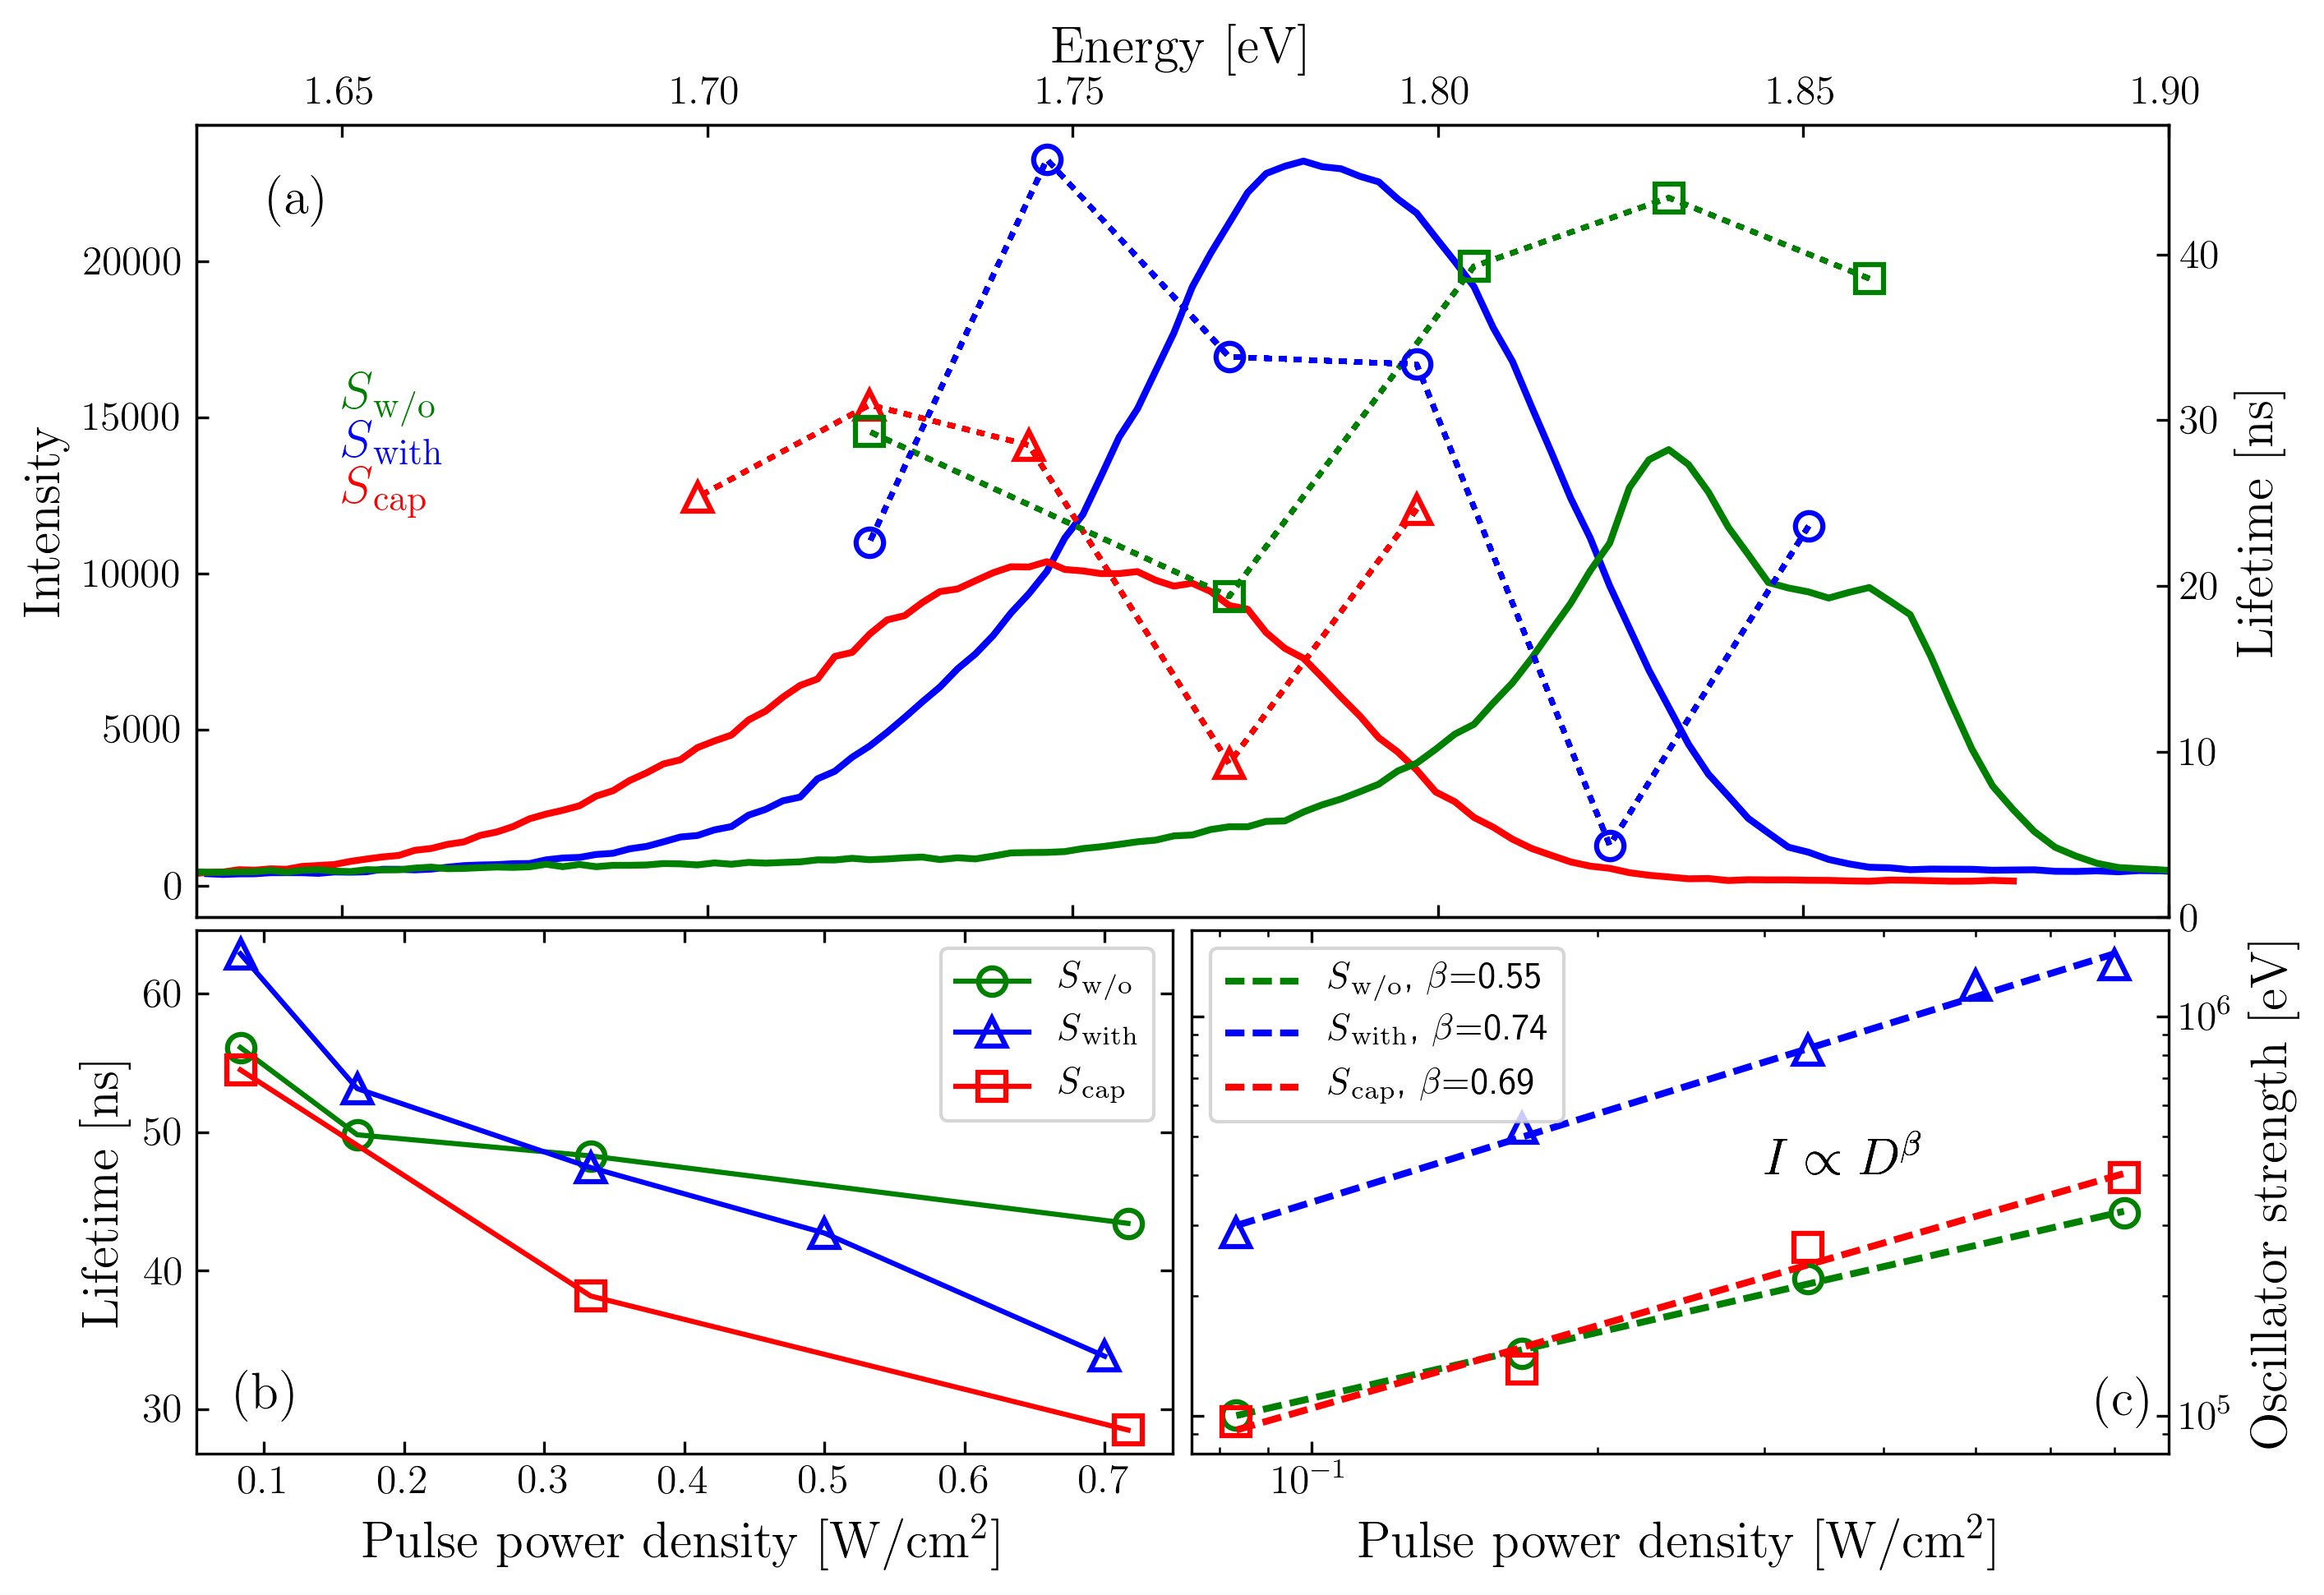
\includegraphics[width=1\linewidth]{/TRPL/intensity/porovnani_vzorku_maximum_int}
\caption{(a) Decay times $\tau_\mathrm{PL}$ (symbols) for the studied samples as a function of the emission energy measured at 15~K and 0.7~W/cm$^2$. Appropriate PL spectra (solid lines) are added for better orientation. Panel~(b) depicts $\tau_\mathrm{PL}$ in the maximum of the PL signal and panel~(c) $\tau_\mathrm{PL}$ for the integrated PL intensity in whole measured range as a function of excitation density for the samples.}
\label{fig:TRPL_int_all}
\end{figure}


\subsection{Excitation intensity dependent TRPL}
The excitation density of the pulse laser was varied in the range 0.08--0.7~W/cm$^2$ (the optical response was in linear regime in the whole varied excitation range for each sample, see Fig.~\ref{fig:TRPL_int_all}(c)), then the measured TRPL signal has been deconvoluted by 2ME decay model, e.~g., Fig.~\ref{fig:TRPL_int_w} depicts TRPL signal in the maximum of PL spectra of $S_\mathrm{with}$). 

We observe a decrease of the fast decay component with increasing excitation density as shown in Fig.~\ref{fig:TRPL_int_w}(b)--(c), which is in agreement with behaviour of type-II nanostructures observed elsewhere~\citep{Ledentsov_prb1995_intmodel,Gu_prb2005_TRPLtype2,Manna_apl2012_TRPLtype2,Zaitsev_prb2007}. At higher excitation intensity, a larger carrier concentration of the photogenerated electron-hole pairs results in band bending, hence a stronger overlap of electron-hole wave-functions, and thus a faster decay.
%

\begin{figure}
	\centering
	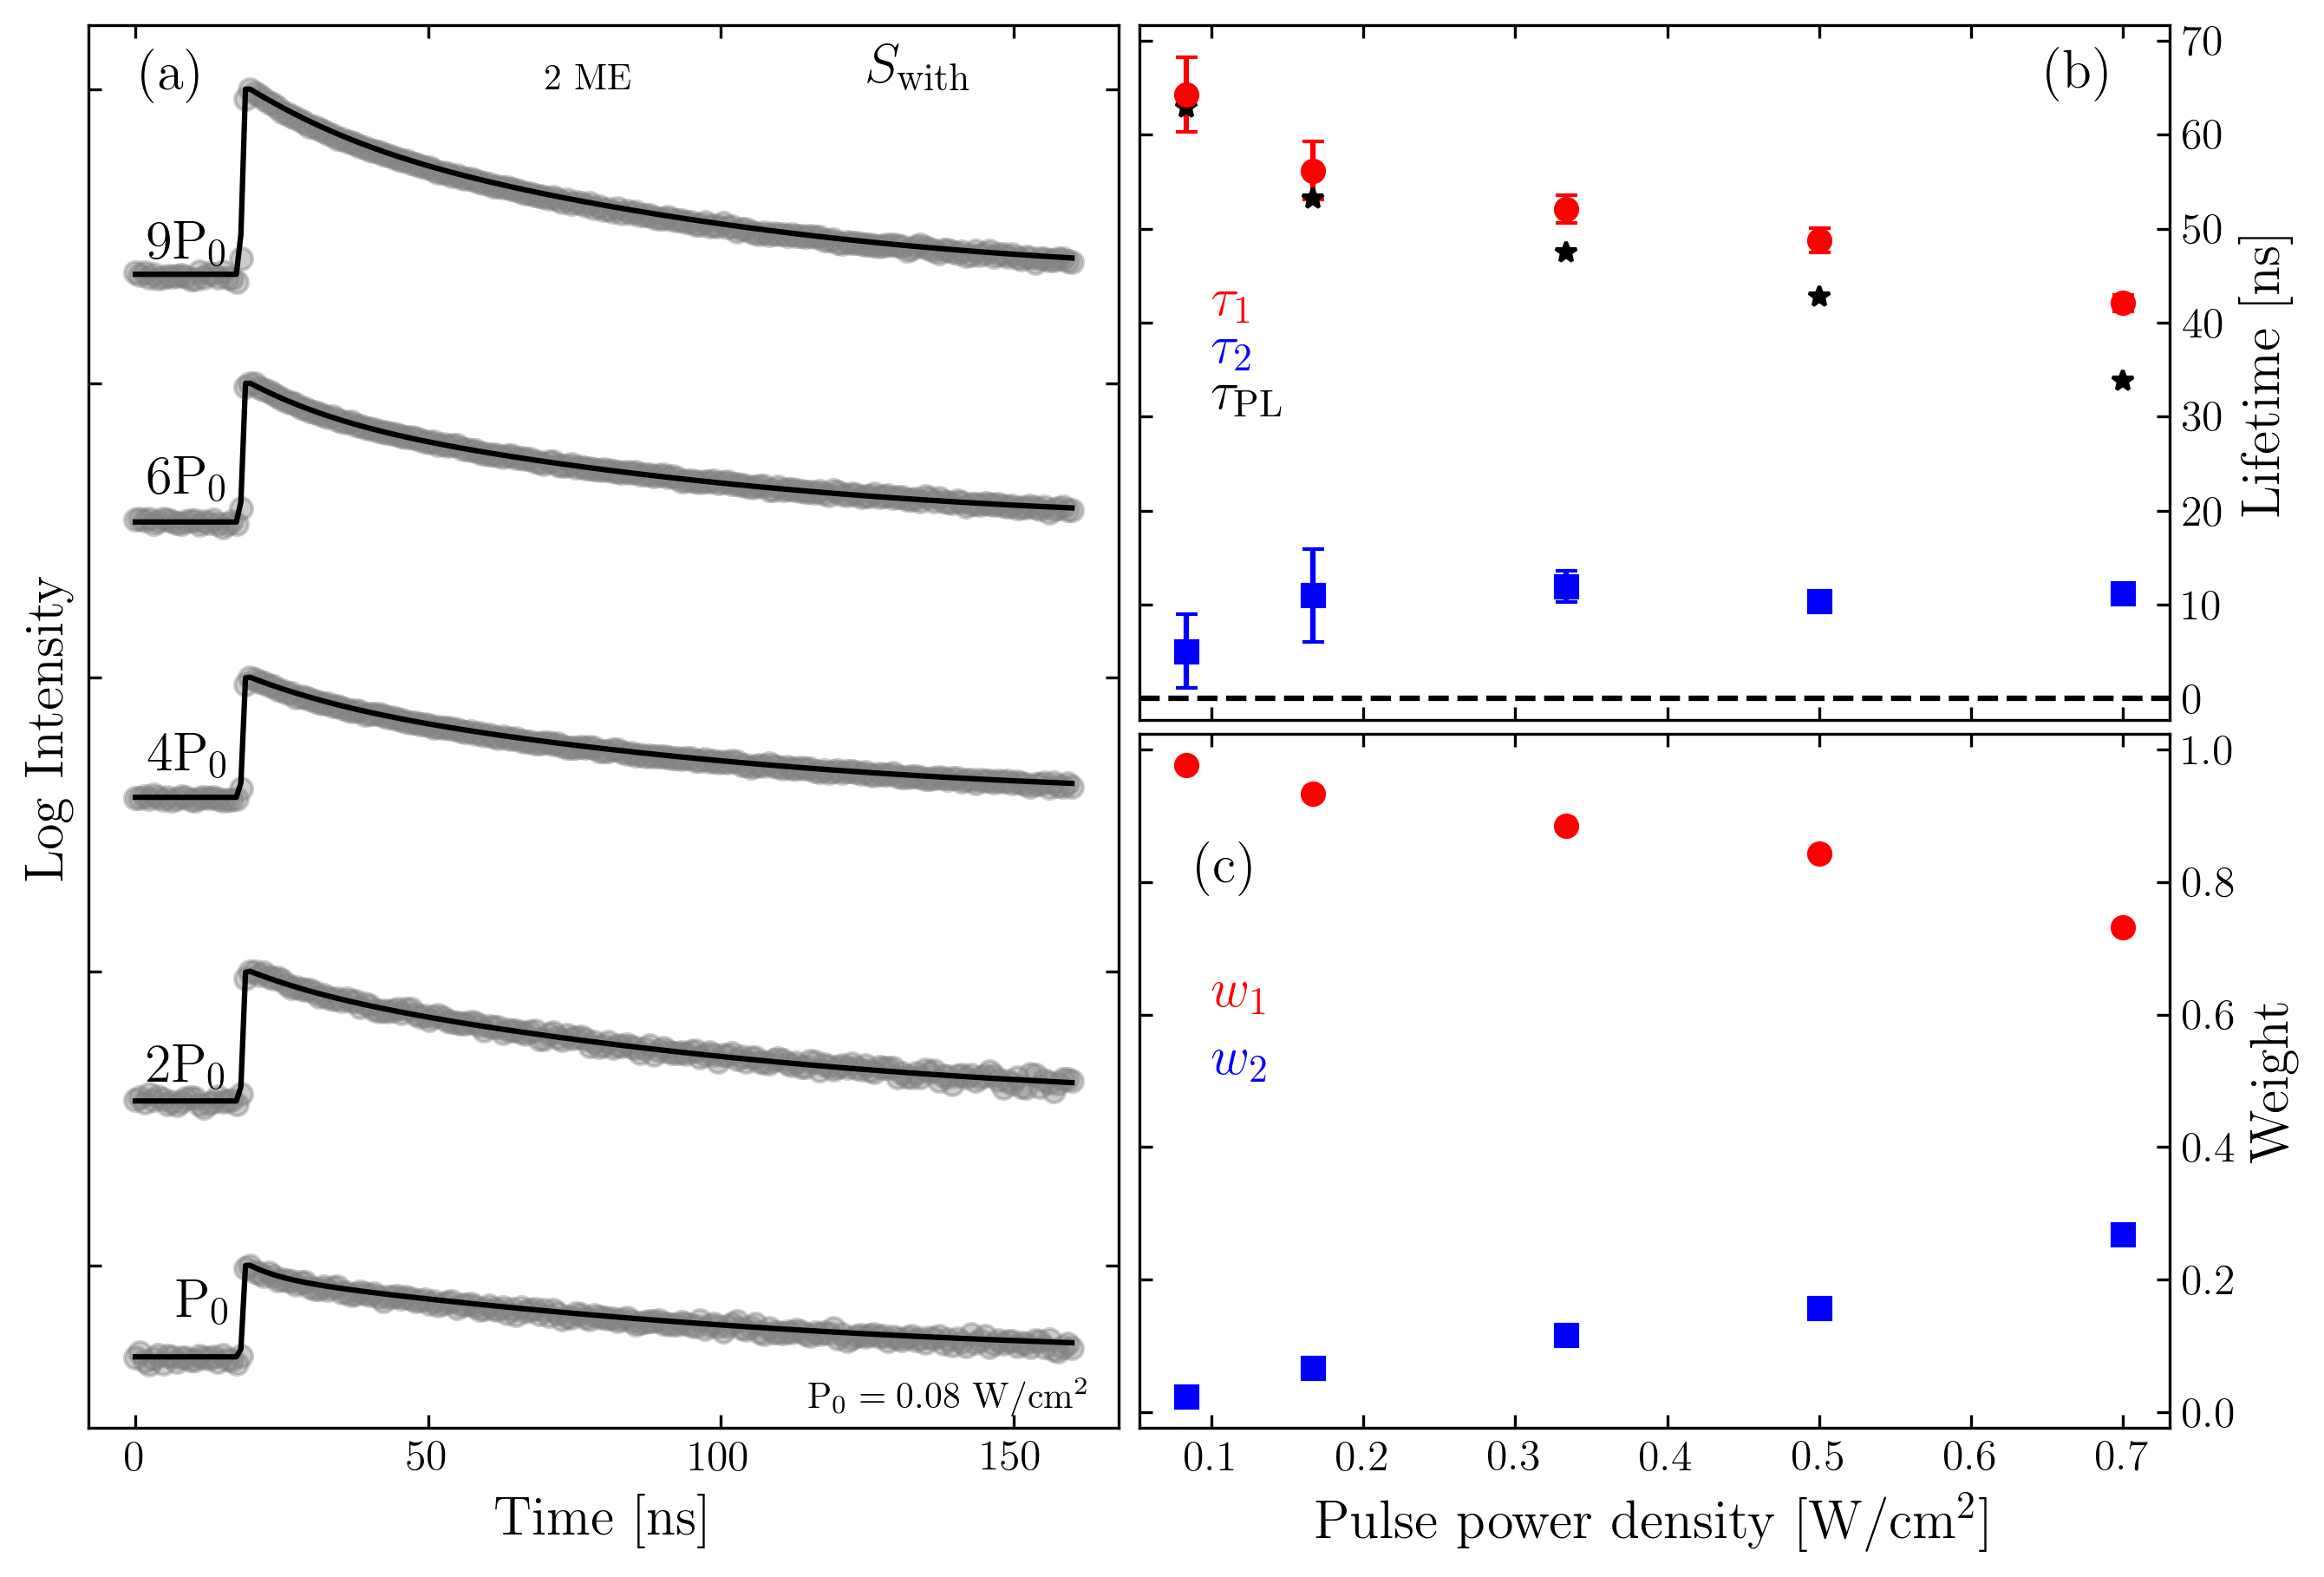
\includegraphics[width=1\linewidth]{/TRPL/intensity/12040_TRPL_Tfw0_int}
	\caption{(a) Experimental TRPL measured at 15~K as a function of excitation density (grey circles) and its deconvolution by 2ME model (solid lines) at the maximum of band $M_1^\mathrm{w}$ for sample $S_\mathrm{with}$. (b) Fitted decay times $\tau_1$ (red circles), $\tau_2$ (blue squares) and characteristic time $\tau_\mathrm{PL}$ (black stars) as a function of excitation density. Appropriate weights are shown in panel (c).}
	\label{fig:TRPL_int_w}
\end{figure}
Other samples given in appendix~\ref{chapter:appendix_TRPL_int} show similar behaviour and with comparable $\tau_\mathrm{PL}$ at low excitation power. However, $\tau_\mathrm{PL}$ of samples with QDs is approximately twice as small, see Fig.~\ref{fig:TRPL_int_all}(b).

\newpage
\subsection{Temperature dependent TRPL}
TRPL variations with temperature are shown in Figs.~\ref{fig:TRPL_temp_wo}-\ref{fig:TRPL_temp_c} and are deconvoluted again by 2ME model. As it can be seen in Fig.~\ref{fig:TRPL_temp_w}, the resulting decay times of sample $S_\mathrm{with}$ increase up to the temperature of 30~K and then progressively reduce which is characteristic of the appearance of thermally activated scape paths~\citep{Manna_apl2012_TRPLtype2}. Contrary to sample $S_\mathrm{with}$, on $S_\mathrm{w/o}$ and $S_\mathrm{cap}$ the reduction of the decay times begins at the lowest temperatures without an increase at the beginning.
%
\begin{figure}
	\centering
	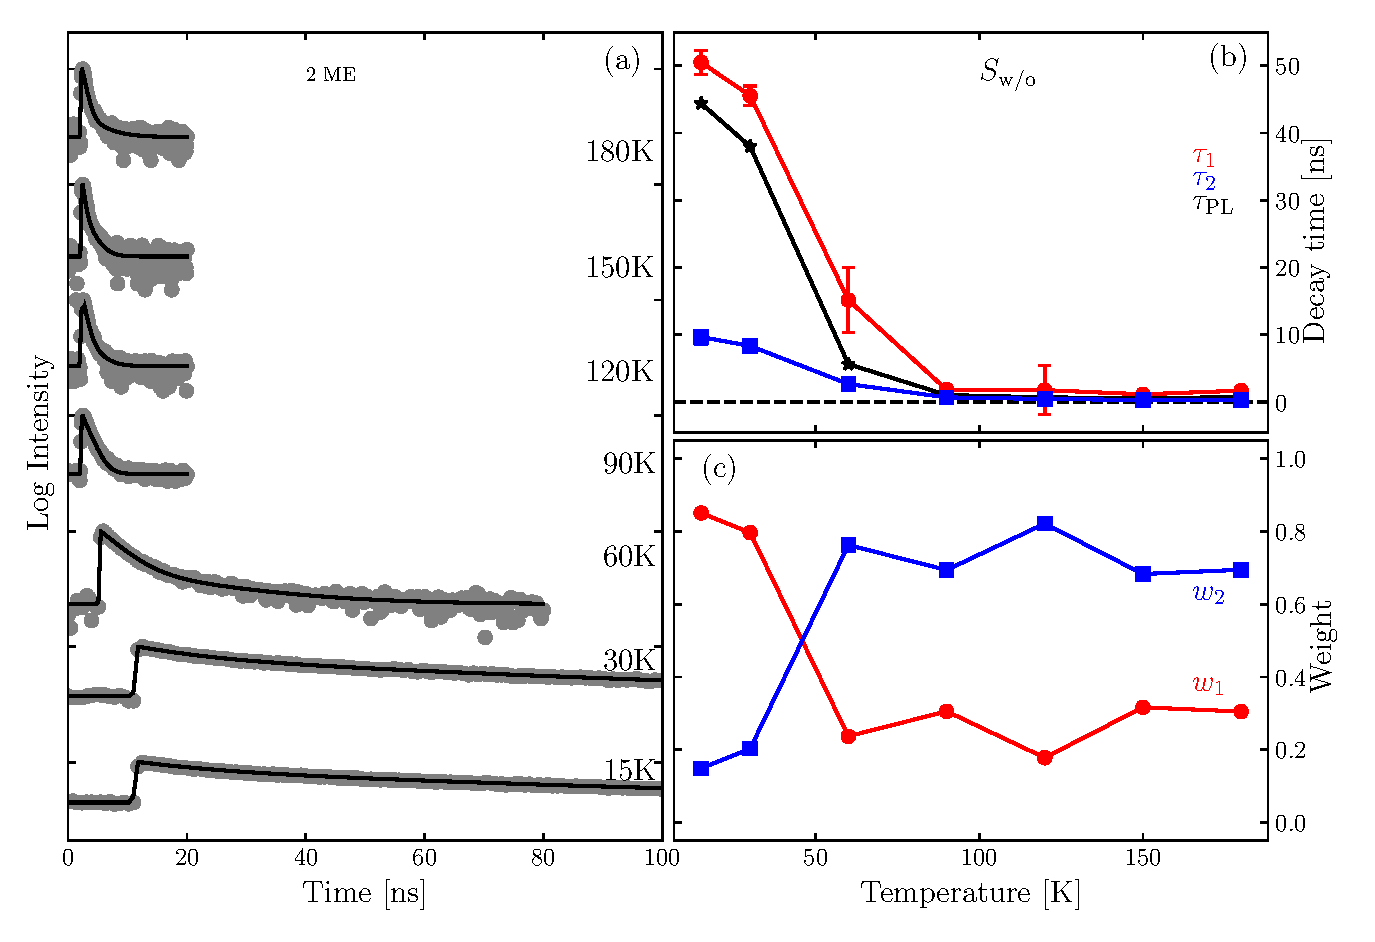
\includegraphics[width=0.9\linewidth]{/TRPL/temperature/12027_TRPL_max677_temp}
	\caption{(a) Experimental TRPL at pumping power of 0.3~W/cm$^2$ as a function of temperature (grey circles) and its deconvolution by 2ME model (solid black lines) at the maximum of PL signal in sample $S_\mathrm{w/o}$. (b) Deconvolved decay times ($\tau_1$: red circles; $\tau_2$: blue squares) and characteristic time $\tau_\mathrm{PL}$ (black stars) as a function of temperature. Corresponding weights are shown in panel (c).}
	\label{fig:TRPL_temp_wo}
\end{figure}
%
\begin{figure}
	\centering
	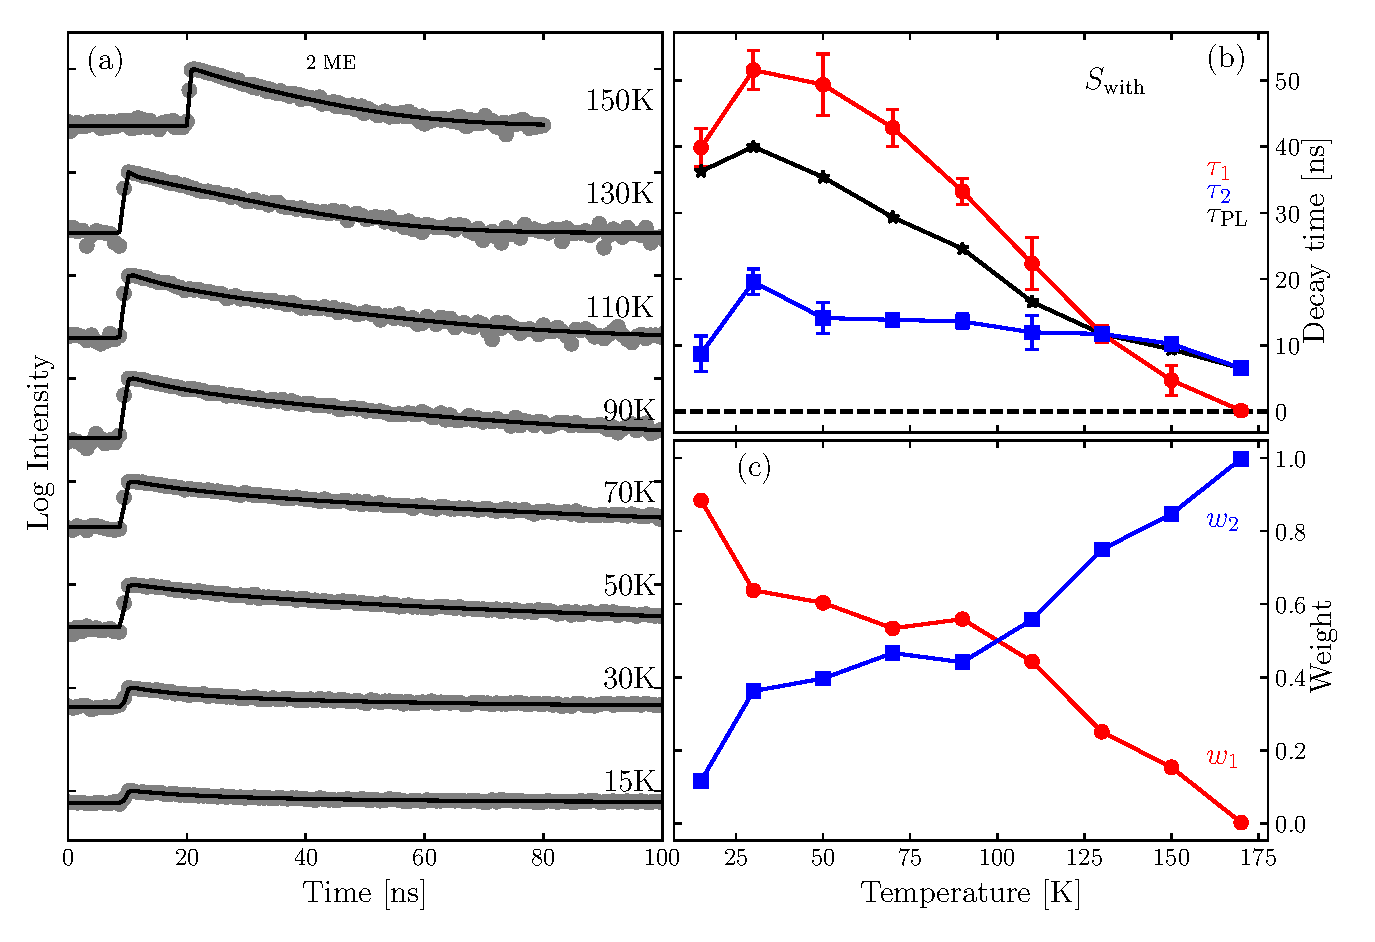
\includegraphics[width=0.9\linewidth]{/TRPL/temperature/12040_TRPL_700-710_temp}
	\caption{TRPL signal as a function of temperature at the maximum of PL in sample $S_\mathrm{with}$ similarly commented as in Fig.~\ref{fig:TRPL_temp_wo}.}
	\label{fig:TRPL_temp_w}
\end{figure}
%

If we assume similarly as in Ref.~\citep{t_alvarez} that at 15~K the only loss mechanism is radiative recombination, the radiative $\tau_\mathrm{R}$ and non-radiative $\tau_\mathrm{NR}$ decay times can be extracted from $\tau_\mathrm{PL}$ by
%
\begin{equation}
\tau_\mathrm{R}=\frac{I_0}{I_\mathrm{PL}(T)}\tau_\mathrm{PL} \label{eq:tau_R_fromPL}
\end{equation}
and
\begin{equation}
\frac{1}{\tau_\mathrm{PL}}=\frac{1}{\tau_\mathrm{R}} + \frac{1}{\tau_\mathrm{NR}}
\end{equation}
%
\begin{figure}
	\centering
	\includegraphics[width=0.9\linewidth]{/TRPL/temperature/12021_TRPL_690_temp}
	\caption{TRPL signal as a function of temperature at the maximum of PL in sample $S_\mathrm{cap}$ similarly commented as in Fig.~\ref{fig:TRPL_temp_wo}.}
	\label{fig:TRPL_temp_c}
\end{figure}
%

\noindent where $I_0$ and $I_\mathrm{PL}$ are the PL intensity at 15~K and that as a function of $T$, respectively. As can be seen in Fig.~\ref{fig:TRPL_temp_decon} $\tau_\mathrm{NR}$ decreases with temperature as is usually the case for thermally activated processes. Parameter $\tau_\mathrm{NR}$ can be fitted with two non-radiative processes 
%
\begin{equation}
\frac{1}{\tau_\mathrm{NR}}=\frac{1}{\tau_\mathrm{NR}^1}\exp{\left(\frac{-E_1}{k_\mathrm{B}T}\right)} + \frac{1}{\tau_\mathrm{NR}^2}\exp{\left(\frac{-E_2}{k_\mathrm{B}T}\right)} \label{eq:nonradiative}
\end{equation}
characterized by activation energies $E_1$ and $E_2$ and time constants $\tau_\mathrm{NR}^1$ and $\tau_\mathrm{NR}^2$, respectively.
Conversely, $\tau_\mathrm{R}$ increases exponentially with temperature
%
\begin{equation}
\tau_\mathrm{R} = \tau_\mathrm{R}^0 + \tau_\mathrm{R}^T \exp{\left(\frac{T}{T_C}\right)}, \label{eq:tau_R} 
\end{equation}
where $ \tau_\mathrm{R}^0$ ($ \tau_\mathrm{R}^T$) describes the temperature independent (dependent) part of the radiative decay and $T_C$ is the characteristic temperature corresponding to the energy of localized states. Inserting Eq.~(\ref{eq:tau_R_fromPL}) into Eq.~(\ref{eq:tau_R}) we can obtain an Arrhenius-like equation with an explicit dependence of the PL intensity on all the parameters derived from the TRPL analysis
%
\begin{equation}
I_\mathrm{PL}(T)=\frac{I_0}{1+\left[\tau_\mathrm{R}^0+\tau_\mathrm{R}^T\exp{\left(\frac{T}{T_C}\right)}\right] \times \left[\frac{1}{\tau_\mathrm{NR}^1}\exp{\left(\frac{-E_1}{k_\mathrm{B}T}\right)} + \frac{1}{\tau_\mathrm{NR}^2}\exp{\left(\frac{-E_2}{k_\mathrm{B}T}\right)}\right]}. \label{eq:TRPL_Arhenius}
\end{equation}
%
\begin{figure}
	\centering
	\includegraphics[width=1\linewidth]{/TRPL/temperature/decay_dekonvolution_all}
	\caption{Characteristic PL decay time $\tau_\mathrm{PL}$ as a function of temperature with the radiative and non-radiative components for all our samples. The radiative and non-radiative component are fitted by Eq.~(\ref{eq:tau_R}) and Eq.~(\ref{eq:nonradiative}), respectively.}
	\label{fig:TRPL_temp_decon}
\end{figure}

As it can be seen in Fig.~\ref{fig:Arrhenius_PLandTRPL}, this formula is equally good in reproducing experimental data as~Eq.~(\ref{eq:Arhenius}). 


\newpage

We now discuss the numerical results obtained in this analysis that are summarized in Tab.~\ref{tab:TRPL_params}. As can be seen in Fig.~\ref{fig:TRPL_temp_decon} the radiative decay time of $S_\mathrm{w/o}$ does not depend on temperature and is described only by $\tau_\mathrm{R}^0=39.6$~ns. On the contrary, the radiative decay time of samples with QDs exponentially grows with temperature and is proportional to similar value, i.~e., $\tau_\mathrm{R}^T=12.0$~ns for $S_\mathrm{with}$ and $11.5$~ns for $S_\mathrm{cap}$, respectively. 
The non-radiative process with smaller activation energy ($E_1$ between 6 and 18~meV) is probably associated with trapping of carriers by impurities or defects in the vicinity of QDs, as it has been also before for InAs/InP quantum wires~\citep{Alen_apl2011}. The other process is characterized by faster time constant $\tau_\mathrm{NR}^2$ ($\tau_\mathrm{NR}^1/\tau_\mathrm{NR}^2>5$) is close to the thermally activated capture of excitions by nonradiative defects in GaAs layer~\citep{Seravallo_apl2005,Kohki_apl1997}. 

The values obtained by fitting the dependencies by model in Eq.~(\ref{eq:TRPL_Arhenius}) are summarized in Tab.~\ref{tab:TRPL_params} and are comparable with parameters gained from the temperature dependence PL data shown in Sec.~\ref{Sec:temp_PL_TU}, which are equally well reproduced by Eq.~\ref{eq:Arhenius}, see the parameters resume in Tab.~\ref{tab:Arhenius}.

The previous temperature dependent TRPL and PL analysis of the samples allow us to draw simple scheme of the time evolution of the levels involved in the exciton dynamics, namely that of the recombining level \textbf{F} and three trap levels \textbf{N$_i$}, see Fig.~\ref{fig:Arrhenius_PLandTRPL}.
\begin{table}
	\centering
	\caption{Summary of the TRPL Arrhenius-like fits. The displayed values are obtained with accuracy better than $10^{-3}\%$.}
	\begin{tabularx}{0.9\textwidth}{cCCccccc}
		\toprule
		
		 & $E_1$ [meV]& $\tau_\mathrm{NR}^1$ [ns]& $E_2$ [meV]& $\tau_\mathrm{NR}^2$ [ns] & $\tau_\mathrm{R}^0$ [ns]& $\tau_\mathrm{R}^T$ [ns]& $T_C$ [K]\\ 	
		\midrule
		\midrule
		$S_\mathrm{w/o}$& 17.5&0.13&294.3 & 0.03& 39.55&0.00&8825.0\\
		$S_\mathrm{with}$&6.7 & 20.10& 47.2&0.30& 26.76&12.00&64.9\\
		$S_\mathrm{cap}$& 10.0&1.33&33.8 & 0.25& 13.32&11.48&76.9\\
		
		\bottomrule
	\end{tabularx}\label{tab:TRPL_params}
\end{table}



\begin{figure}
	\centering
	\includegraphics[width=0.9\linewidth]{/TRPL/temperature/models} %Arrhenius_PLandTRPL_all}
	\caption{The left panels (a)-(c) compare the integrated PL intensity and the corresponding fit for all our samples of the measurements performed with a CW (circles) and a pulsed (squares) laser. The right panels show levels involved in the exciton dynamics in our samples. The letters \textbf{0} and \textbf{F} in these sketches represent the vacuum end exciton state, respectively, \textbf{N$_i$} are three trap levels.}
	\label{fig:Arrhenius_PLandTRPL}
\end{figure}
\newpage 

%%% -------------------------------------------------------------
\appendix
\chapter{Material parameters used in 8-band $\bf{k \cdot p}$ calculations of InGaAs QDs} \label{app:material_params}

\begin{table*}[!ht]
	\caption{Values of the material parameters used in the calculations. The labeling is defined in Tab.~\ref{tDesc} and the references from which the parameters were taken are identified in the last column.\label{tSb2} 
		}
	\begin{center}
		\begin{tabular}{llccc}
			\hline \hline
			Parameter & Unit & InAs & GaAs & Ref.\\
			\hline
			$a$ & \AA & $6.0583$ & $5.6533$  & \cite{Vurgaftman}\\
			$a_{exp}$ & \AA /K& $2.74\times$10$^{-5}$ & $3.88\times$10$^{-5}$  & \cite{Vurgaftman}\\
			$C_{11}$ & GPa& $83.29$ & $122.1$  & \cite{Vurgaftman}\\
			$C_{12}$ & GPa& $45.26$ & $56.6$  & \cite{Vurgaftman}\\
			$C_{44}$ & GPa& $39.59$ & $60.0$ & \cite{Vurgaftman}\\
			$E_0$ & eV & $0.417$ & $1.519$ &  \cite{Vurgaftman}\\
			$\alpha$ & eV/K & $0.276\times$10$^{-3}$ & $0.541\times$10$^{-3}$ &  \cite{Vurgaftman}\\
			$\beta$ & K & $93$ & $204$ & \cite{Vurgaftman}\\
			$E_v$ & eV & $1.390$ & $1.346$ &  \cite{zunger}\\
			$\Delta_0$ & eV & $0.390$ & $0.341$ &  \cite{Vurgaftman}\\
			$a_c$ & eV & $-6.66$ & $-9.36$ & \cite{zunger}\\
			$a_v$ & eV & $-1.00$ & $-1.21$ & \cite{zunger}\\
			$a_{ub}$ & eV & $-1.8$& $-2.0$&  \cite{Vurgaftman}\\
			$a_{ud}$ & eV & $-3.6$& $-4.8$&  \cite{Vurgaftman}\\
			$S$ & -& $-4.80$ & $-2.88$ & \cite{Vurgaftman}\\
			$E_p$ & eV & $21.5$ & $28.8$ & \cite{Vurgaftman}\\
			$L$ & $\hbar^2/2m_0$ & $-15.695$ & $1.420$ & \cite{Vurgaftman}\\
			$M$ & $\hbar^2/2m_0$ & $-4.0$ & $-3.9$ & \cite{Vurgaftman}\\
			$N$ & $\hbar^2/2m_0$ & $-15.895$ & $0.056$ & \cite{Vurgaftman}\\
			\hline \hline
		\end{tabular}
	\end{center}
\end{table*}

% InAs  8x8kp-parameters                    = -10.4627d0 -4.0d0   -10.6627d0 ! L',M,N' [hbar^2/2m] (--> divide by hbar^2/2m)
%\newpage

\begin{table*}[!ht]
	\caption{Composition dependence of the input parameters of $\mathrm{In_xGa_{1-x}As}$ used in the calculations. The labeling of parameters is defined in Tab.~\ref{tDesc}. The references from which parameters were taken are identified in the last column. Those parameters whose reference is missing were provided by the parameter library of nextnano++~\cite{next}.\label{tSb3}
	}
	\begin{center}
		\begin{tabular}{llcc}
			\hline \hline
			Parameter & Unit & $\mathrm{In_xGa_{1-x}As}$ & Ref.\\
			\hline
			$a$ & \AA & linear & \\
			$a_{exp}$ & \AA /K & linear & \\
			$C_{11}$ & GPa& linear &  \\
			$C_{12}$ & GPa& linear &  \\
			$C_{44}$ & GPa& linear & \\
			%$e_{14}$ & C/m$^2$ & linear & \\
			$\varepsilon_{r}$ & -& linear & \\
			$E_0$ & eV & $0.417x+1.519(1-x)-0.477x(1-x)$ & \cite{Vurgaftman}\\
			$\alpha$ & eV/K & linear & \\
			$\beta$ & K & linear & \\
			$E_v$ & eV & $1.39x+1.346(1-x)+0.38x(1-x)$& \cite{Vurgaftman}\\
			$\Delta_0$ & eV & $0.39x+0.341(1-x)-0.15x(1-x)$& \cite{Vurgaftman}\\
			$a_c$ & eV & $-6.66x-9.36(1-x)-2.61x(1-x)$& \cite{Vurgaftman}\\
			$a_v$ & eV & linear & \\
			$a_{ub}$ & eV & linear& \\
			$a_{ud}$ & eV & linear& \\
			$S$ & -& $-4.80x-2.88(1-x)-3.54x(1-x)$& \cite{Vurgaftman}\\
			$E_p$ & eV & $21.5x+28.8(1-x)+1.48x(1-x)$& \cite{Vurgaftman}\\
			$L$ & $\hbar^2/2m_0$ & $-15.695x+1.420(1-x)+25.063x(1-x)$& \cite{Vurgaftman}\\
			$M$ & $\hbar^2/2m_0$ & $-4.0x-3.86(1-x)+1.141x(1-x)$& \cite{Vurgaftman}\\
			$N$ & $\hbar^2/2m_0$ & $-15.895x+0.056(1-x)+26.809x(1-x)$& \cite{Vurgaftman}\\
			\hline \hline
		\end{tabular}
	\end{center}
\end{table*}

\newpage 
\chapter{Derivation of the relation between in-plane stress in principal and Cartesian coordinates}
\label{app:principal_stress}

Any in-plane stress configuration can be described by three independent components of stress tensor ($\sigma_{xx}$, $\sigma_{yy}$, and $\sigma_{xy}$) or, equivalently, by two principal stresses $\sigma_\mathrm{max}$ and $\sigma_\mathrm{min}$ applied at an angle $\alpha$ with respect to the crystal axis. We now introduce the connection between the Cartesian and principal components.

We first rotate the basis of the stress components $\sigma_{xx}$, $\sigma_{yy}$ and $\sigma_{xy}$ by an angle $\theta$ to obtain components $\sigma_{xx}'$, $\sigma_{yy}'$ and $\sigma_{xy}'$ in the rotated basis which are related to the previous ones by
%
\begin{align}
\sigma_{xx}' &= \sigma_{xx}\cos^2{\theta}+\sigma_{yy}\sin^2{\theta}+2\sigma_{xy}\sin{\theta}\cos{\theta} , \\
\sigma_{yy}' &=\sigma_{xx}\sin^2{\theta}+\sigma_{yy}\cos^2{\theta}-2\sigma_{xy}\sin{\theta}\cos{\theta}, \\
\sigma_{xy}' &=\left(\sigma_{xx}-\sigma_{yy}\right)\sin{\theta}\cos{\theta}+\sigma_{xy}\left(\cos^2{\theta}-\sin^2{\theta}\right).
\end{align}
%
%
%
%
Principal stress orientation can be then computed by setting $\sigma_{xy}'=0$ in the last equation and solving
%
%
\begin{equation}
\sigma_{xx}\sin^2{\theta}+\sigma_{yy}\cos^2{\theta}-2\sigma_{xy}\sin{\theta}\cos{\theta}=0,
\end{equation}
%
%
for $\theta$. The result is the equation giving the principal stress angle which we denote $\alpha$
%
%
\begin{equation}
\tan{2\alpha}=\frac{2\sigma_{xy}}{\sigma_{xx}-\sigma_{yy}}\label{eq:principal_angle}.
\end{equation}
%
Inserting $\alpha$ back into the Eqs.~(1)--(3) we obtain the principal stress values $\sigma_\mathrm{max}$ and $\sigma_\mathrm{min}$
%
%
\begin{equation}
\sigma_\mathrm{max}, \sigma_\mathrm{min} = \frac{\sigma_{xx}+\sigma_{yy}}{2} \pm \sqrt{\left(\frac{\sigma_{xx}-\sigma_{yy}}{2}\right)^2+\sigma_{xy}^2}. \label{eq:princip_strain}
\end{equation}
%
%



We then express the sum and the difference of $\sigma_\mathrm{max}$ and $\sigma_\mathrm{min}$
%
\begin{align}
\sigma_{\mathrm{max}}+\sigma_{\mathrm{min}} &= \sigma_{xx}+\sigma_{yy}, \label{eq:plus}\\
\sigma_{\mathrm{max}}-\sigma_{\mathrm{min}} &= \sqrt{\left(\sigma_{xx}-\sigma_{yy}\right)^2+4\sigma_{xy}^2}.\label{eq:minus}
\end{align}
%
If we now combine equations (\ref{eq:princip_strain}) with (\ref{eq:minus}) we can write
%
%
\begin{equation}
\label{eq:nxyVSnprinc}
\sigma_{xy}=\frac{1}{2}\left(\sigma_{\mathrm{max}}-\sigma_{\mathrm{min}}\right)\sin{2\alpha}.
\end{equation}
%

\newpage 
\chapter{Slopes of dipole ${p}$ for stress-tuned InGaAs quantum dots}
\label{app:slopes_of_dipole}
	

	
	The dependencies of $1/e\times p \left( \sigma_\mathrm{max}+\sigma_\mathrm{min} \right)$ were fitted by linear function $ A^{\mathrm{QD}}\left(\sigma_\mathrm{max} + \sigma_\mathrm{min}\right) + b$. %The meaning of fitting parameters is $a=A^{\mathrm{QD}}$ and $b=A^{\mathrm{QD}}\sigma^{\mathrm{pre}}_{xy}$.
	%
	%Dependencies of $E_0$ (top panel) and $p/e$ (bottom panel) on $\sigma_{\mathrm{max}}+\sigma_{\mathrm{min}}$ experimentally obtained from $\mu$PL measurements of nine InGaAs QDs~\cite{Aberl:17} (broken curves) and that calculated for different values of dot height. Except of height the simulated QDs had the same properties as QD$_2$ including the value of $\sigma^{\mathrm{pre}}=200$~MPa. The letter $e$ denotes the elementary charge.
	%
	%
	
	\begin{table}[ht!]
		\centering
		\caption{Fitted slopes of $A^{\mathrm{QD}}$ for experimental data shown in Sec.~\ref{chap:2order_piezo}.}
		\label{tab:exp_slopes}
		\begin{tabular}{|c|c|c|}
			\hline
			& $A^{\mathrm{QD}}$  [nm/GPa]    & b   [nm]    \\ \hline
			\multirow{9}{*}{Experiment} & $-0.43$ $\pm$ $0.02$  & $-0.066$ $\pm$ $0.002$      \\ \cline{2-3}
			& $-0.46 \pm 0.01$  & $-0.039 \pm 0.002$      \\ \cline{2-3}
			& $-0.41 \pm 0.01$  & $-0.055 \pm 0.001$      \\ \cline{2-3}
			& $-0.42 \pm 0.01$  & $-0.123 \pm 0.001$      \\ \cline{2-3}
			& $-0.42 \pm 0.01$  & $-0.174 \pm 0.002$      \\ \cline{2-3}
			& $-0.47 \pm 0.04$  & $-0.094 \pm 0.004$      \\ \cline{2-3}
			& $-0.38 \pm 0.01$  & $-0.202 \pm 0.001$      \\ \cline{2-3}
			& $-0.46 \pm 0.02$  & $-0.171 \pm 0.002$      \\ \cline{2-3}
			& $-0.50 \pm 0.02$  & $-0.083 \pm 0.002$      \\ \hline
		\end{tabular}    
	\end{table} 
	
 		\begin{table}[ht!]
 			\centering
 			\caption{Fitted slopes of $A^{\mathrm{QD}}$ for different In concentration profiles, data are shown in Fig.~\ref{fig:TuningByConc}.}
 				\label{tab:conc_slopes}
 				\begin{tabular}{|c|c|c|c|}
 					\hline
 		In content (base--apex)	[$\%$]	& Piezo order	& $A^{\mathrm{QD}}$ [nm/GPa]    & b   [nm]    \\ \hline
 					\multirow{2}{*}{$0.25-0.65$} & $2^\mathrm{nd}$ piezo &$-0.430 \pm 0.003$  & $-0.0325 \pm 0.0003$      \\ \cline{2-4}
 			&	$1^\mathrm{st}$ piezo 	& $-0.065 \pm 0.001$  & $0.0951 \pm 0.0006$      \\ \hline
 			%
 			\multirow{2}{*}{$0.65-0.25$} & $2^\mathrm{nd}$ piezo &$-0.546 \pm 0.001$  & $-0.2616 \pm 0.0001$      \\ \cline{2-4}
 			&	$1^\mathrm{st}$ piezo 	& $-0.101 \pm 0.001$  & $-0.0945 \pm 0.0001$      \\ \hline
 			%
 			\multirow{2}{*}{$0.45-0.45$} & $2^\mathrm{nd}$ piezo &$-0.626 \pm 0.001$  & $-0.2038 \pm 0.0002$      \\ \cline{2-4}
 			&	$1^\mathrm{st}$ piezo 	& $-0.113 \pm 0.010$  & $-0.0087 \pm 0.0001 $     \\ \hline
 				\end{tabular}    
 			\end{table}
 			

 		\begin{table}[ht!]
 			\centering
 			\caption{Fitted slopes of $A^{\mathrm{QD}}$ for various height of QD, data shown in Fig.~\ref{fig:TuningByHeight}. The data were obtained with the expansion of the piezo-electric field up to second order in strain.}
 			\label{tab:height_slopes}
 			\begin{tabular}{|c|c|c|}
 				\hline
 				Height [nm]		& $A^{\mathrm{QD}}$ [nm/GPa]    & b   [nm]    \\ \hline
 			 $1.5$  &$-0.319 \pm 0.003$  & $-0.0764 \pm 0.0004$     \\ \hline
 			$2.0$	&$-0.313 \pm 0.003$  & $-0.0594 \pm 0.0006$      \\ \hline
 			 $2.5$  &$-0.353 \pm 0.003$  & $-0.0452\pm 0.0003$     \\ \hline
 			 $3.0$	&$-0.430 \pm 0.003$  & $-0.0325 \pm 0.0003$      \\ \hline
 			 $3.5$  &$-0.531 \pm 0.004$  & $-0.0149\pm 0.0004$     \\ \hline
 			 $4.0$	&$-0.658 \pm 0.005$  & $0.0047 \pm 0.0005$      \\ \hline
 				%
 			\end{tabular}    
 		\end{table}
 		

 		\begin{table}[ht!]
 			\centering
 			\caption{Fitted slopes of $A^{\mathrm{QD}}$ for various applied pre-stress, data shown in Fig.~\ref{fig:TuningByPrestress}. The data were obtained with the expansion of the piezo-electric field up to second order in strain.}
 			\label{tab:prestress_slopes}
 			\begin{tabular}{|c|c|c|}
 				\hline
 				Pre-stress $\sigma^\mathrm{pre}$ [MPa]		& $A^{\mathrm{QD}}$ [nm/GPa]    & b   [nm]    \\ \hline
 				$50$  &$-0.337 \pm 0.003$  & $0.1039 \pm 0.0003 $    \\ \hline
 				$100$	&$-0.334 \pm 0.003$  & $0.0846 \pm 0.0003 $     \\ \hline
 				$200$  &$-0.376 \pm 0.003$  & $0.0406\pm 0.0003 $    \\ \hline
 				$350$	&$-0.430 \pm 0.003$  & $-0.0325 \pm 0.0003$      \\ \hline
 				$400$  &$-0.446 \pm 0.003$  & $-0.0584 \pm 0.0003$    \\ \hline
 				$500$	&$-0.476 \pm 0.003$  & $-0.1210 \pm 0.0003$      \\ \hline
 				%
 			\end{tabular}    
 		\end{table}
 		
 		
 		
 		\begin{table}[ht!]
 			\centering
 			\caption{Fitted slopes of $A^{\mathrm{QD}}$ for different aspect of truncated dot (ratio of top and base radius), data shown in Fig.~\ref{fig:TuningByPrestress}.}
 			\label{tab:aspect_slopes}
 			\begin{tabular}{|c|c|c|}
 				\hline
 				Aspect (top/height) 	& $A^{\mathrm{QD}}$ [nm/GPa]    & b   [nm]    \\ \hline
 				1/4	&$-0.343\pm0.005$ &	$0.0546	\pm	0.0005$\\ \hline
 				2/4	&$-0.430\pm0.003$ &	$-0.0325 \pm		0.0003$\\ \hline
 				3/4	&$-0.518\pm0.003$ &	$-0.0928	\pm 0.0003$\\ \hline
 				%
 			\end{tabular}    
 		\end{table}
 		
 		\begin{table}[ht!]
 			\centering
 			\caption{Fitted parameters $A^{\mathrm{QD}}$ and $b$ for QD with various lateral dimension with respect ratio top/base radius of 1/2. Linear fits are presented in Fig.~\ref{fig:TuningByPrestress}.}
 			\label{tab:lateral_slopes}
 			\begin{tabular}{|c|c|c|}
 				\hline
 				Base radius [nm]	& $A^{\mathrm{QD}}$ [nm/GPa]    & b   [nm]    \\ \hline
			20&	$-0.341\pm0.003$&	$0.0333\pm		0.0003$\\ \hline
			30&	$-0.394\pm0.003$&	$-0.0046\pm	0.0003$\\ \hline
			40&	$-0.430\pm0.003$&	$-0.0325	\pm	0.0003$ \\ \hline
 				%
 			\end{tabular}    
 		\end{table}
 		
\newpage
\section*{Evolution of fitted parameters from dependency $p/e = A^\mathrm{QD} \left(\sigma_\mathrm{max}+\sigma_\mathrm{mix}\right) + b$}
%
\label{app:empirical_model}

 		
 		\begin{table}[ht!]
 			\centering
 			\caption{The parameters $A^\mathrm{QD}$ and $b$ can be expand into terms of $\sigma^\mathrm{pre}$: $A^\mathrm{QD}=a_1\sigma^\mathrm{pre}+a_0$ and $b=b_1\sigma^\mathrm{pre}+b_0$, respectively.}
 			\label{tab:prestress_fit}
 			\begin{tabular}{|c|c|c||c|c|}
 				\hline
 				$h$ [nm]		   & $a_1$   [nm GPa$^{-2}$]  &$a_0$ [nmGPa$^{-1}$] & $b_1$ [nmGPa$^{-1}$] & $b_0$ [nm] \\ \hline
 				%$3.0$   & -0.33 $\pm$ 0.02  &  -0.311 $\pm$ 0.006 & -0.48 $\pm$ 0.01 & 0.132$\pm$0.003 \\ \hline
 			$2.0$   & $-0.25 \pm 0.01$  &  $-0.223 \pm 0.002$ & $-0.34 \pm 0.01$ & $0.056\pm0.003$ \\ \hline % po pridani pre=0
 			%
 			$3.0$   & $-0.36 \pm 0.02$  &  $-0.302 \pm 0.004$ & $-0.47 \pm 0.01$ & $0.129\pm0.003$ \\ \hline % po pridani pre=0
 				%
 			$4.0$   & $-0.62 \pm 0.02$  &  $-0.436 \pm 0.004$ & $-0.72 \pm 0.02$ & $0.251\pm0.006$ \\ \hline % po pridani pre=0
 			\end{tabular}    
 		\end{table}
 		
 		
 		
 		\begin{table}[ht!]
 			\centering
 			\caption{The parameters $A^\mathrm{QD}$ and $b$ can be expand into terms of $h$: $A^\mathrm{QD}=a_2h^2+a_1h+a_0$ and $b=b_2h^2 + b_1h+b_0$, respectively.}
 			\label{tab:height_fit}
 			\begin{tabular}{|c|c|c|c|}
 				\hline
 				 $\sigma^\mathrm{pre}$ [MPa]		& $a_2$ [GPa$^{-1}$nm$^{-1}$]    & $a_1$   [GPa$^{-1}$]  &$a_0$ [nmGPa$^{-1}$] \\ \hline
 				$50$  &$-0.042 \pm 0.004$  & $0.13 \pm 0.02$  &  $-0.36 \pm 0.03$ \\ \hline
 				%
 				$200$  &$-0.050 \pm 0.004$  & $0.16 \pm 0.02$  &  $-0.39 \pm 0.03$ \\ \hline
 				%
 				$350$  &$-0.065 \pm 0.004$  & $0.22 \pm 0.02$  &  $-0.50 \pm 0.03$  \\ \hline
 				%
 				 $500$  &$-0.080 \pm 0.005$  & $0.29 \pm 0.03$  &  $-0.61 \pm 0.04$ \\ \hline
 				 %
 			 				\hline
 			 				$\sigma^\mathrm{pre}$ [MPa]	 & $b_2$ [nm$^{-1}$] & $b_1$ [-] & $b_0$ [nm] \\ \hline
 			 				$50$  &$0.021\pm0.001$ &$-0.039 \pm 0.001$ & $0.032\pm0.001$ \\ \hline
 			 				%
 			 				$200$   & $0.012\pm0.001$ &$-0.013 \pm 0.001$ & $-0.033\pm0.005$ \\ \hline
 			 				%
 			 				$350$  & $0.002\pm0.001$ &$-0.021 \pm 0.007$ & $-0.11\pm0.01$ \\ \hline
 			 				%
 			 				$500$  & $-0.011\pm0.002$ &$0.066 \pm 0.002$ & $-0.21\pm0.01$ \\ \hline
 			 				%
 			 			\end{tabular}   
 		\end{table}
 		


\chapter{Photoluminescence results on a variety of InAs/GaAsSb/GaAs samples}


\label{chapter:appendix_SciRep}
\begin{figure}
	\centering
	\includegraphics[width=0.72\linewidth]{/Sci_rep/suplament/osc}
	\caption{Summary of slopes $a_F$ of the linear fit of $F(P)$ for $X^0$ (blue circles), $X^-$ (red triangles), $XX^0$ (green squares), and that for the transition between bulk GaAs and CL (black pentagons). The data are shown for four samples with InGaAs/GaAsSb/GaAs QDs, marked as A through D on the horizontal axis and the sample with InAs/GaAs QDs marked by I; different numbers correspond to a different position on the corresponding sample. The slopes $a_{\rm F}$ were normalised so that $a_{\rm F}=1$ for $X^0$. The dotted vertical line divides QDs corresponding to type-II and type-I confinement, respectively. The horizontal lines mark the values of the slopes for free non-interacting exciton (dashed) and free non-interacting biexciton (dotted).}
	\label{fig:sup:osc_slope}
\end{figure}




\begin{figure}[!ht]
	\centering
	\includegraphics[width=0.72\linewidth]{/Sci_rep/suplament/mean_shift}
	\caption{Summary of the mean blue-shifts $\overline{\Delta E/\Delta P}$. The marking of the data is the same as in Fig.~\ref{fig:sup:osc_slope} except for the dashed horizontal line marking zero value and the dash-dotted horizontal one marking energy shift of $\overline{\Delta E/\Delta P}=0.007$ according to which we distribute the QD samples to those having type-I (or q-type-I) confinement and those presenting with type-II transition, respectively.}
	\label{fig:sup:mean_blueshift}
\end{figure}

\begin{figure}[!h]
	\centering
	\includegraphics[width=0.72\linewidth]{/Sci_rep/suplament/blue-shift}
	\caption{Summary of the mean exponents $\bar{a}_{\Delta E/\Delta P}$ of $\Delta E\propto P^a$ dependence used for fitting of the $E(P)$ data. The marking is the same as in Fig.~\ref{fig:sup:mean_a_blueshift}.}
	\label{fig:sup:mean_a_blueshift}
\end{figure}



\begin{figure}
	\centering
	\includegraphics[width=0.72\linewidth]{/Sci_rep/suplament/polar}
	\caption{Summary of the azimuth $\alpha_{\mathrm{max}}$ and degree $C_{\mathrm{max}}$ of the polarization anisotropy of the multi-particle bands. The marking of the data is the same as in Figs.~\ref{fig:sup:osc_slope}. For each complex the upper panel corresponds to $\alpha_{\mathrm{max}}$ and the lower one to $C_{\mathrm{max}}$.}
	\label{fig:sup:pol}
\end{figure}
\newpage 
\chapter{More information from TEM and EDX experiments}
\label{chapter:appendix_TEM}
We measured TEM together with EDX to get information on the chemical composition of sample S$_\mathrm{cap}$. The results shown in Fig.~\ref{fig:TEM_app} confirm the constituents given in Fig.~\ref{fig:TUstructure}.


\begin{figure}
	\centering
	\includegraphics[width=0.77\linewidth]{/TEM/TEM_appendix/TEM_12040}
	\caption{(a) TEM image measured under bright field conditions using the (200) reflection perpendicular to the growth direction. (b) EDX map in Al which is present only in Al$_{0.4}$GaP layer.}
	\label{fig:TEM_app}
\end{figure}

The emission EDX spectrum (Fig.~\ref{fig:EDX}) shows all elements present in S$_\mathrm{cap}$ sample, i.~e., Ga, P, In, As, Sb, Al; oxygen is detected due to degradation of the sample by oxidation processes; Co, Fe and Zr are typical compounds used in TEM objectives. In Fig.~\ref{fig:concentration_appendix} the distribution of the concentration in the vertical cut is shown, Al$_{0.4}$GaP layer and QD areas are located between 250 and 280$\,$nm and around 80$\,$nm, respectively.
\begin{figure}
	\centering
	\includegraphics[width=0.77\linewidth]{/TEM/TEM_appendix/EDX}
	\caption{EDX spectrum measured on S$_\mathrm{cap}$.}
	\label{fig:EDX}
\end{figure}


\begin{figure}
	\centering
	\includegraphics[width=0.77\linewidth]{/TEM/TEM_appendix/concentration}
	\caption{Atomic fraction as a function of position in the vertical cut (the zero position is associated with the surface of the sample).}
	\label{fig:concentration_appendix}
\end{figure}

\newpage 
\chapter{Time-resolved photoluminiscence of In$_{1-x}$Ga$_{x}$As$_y$Sb$_{1-y}$/GaAs/GaP QDs samples}

\section{Excitation density TRPL}
\label{chapter:appendix_TRPL_int}
\begin{figure}
	\centering
	\includegraphics[width=0.9\linewidth]{/TRPL/intensity/12027_TRPL_max677_int}
	\caption{(a) TRPL measured at 15~K as a function of excitation density (grey circles) and its deconvolution by 2~ME model (solid lines) at the maximum of band $M_1^\mathrm{w/o}$ in the sample $S_\mathrm{w/o}$. (b) Fitted decay times $\tau_1$ (red circles), $\tau_2$ (blue squares) and characteristic time $\tau_\mathrm{PL}$ (black stars) as a function of excitation density. Appropriate weights are visualized in panel (c).}
	\label{fig:TRPL_int_wo}
\end{figure}


\begin{figure}
	\centering
	\includegraphics[width=0.9\linewidth]{/TRPL/intensity/12021_TRPL_max710_int}
	\caption{TRPL spectra of the maximum of band $M_1^\mathrm{c}$ in sample $S_\mathrm{cap}$. The results are given in the same nomenclature as in Fig.~\ref{fig:TRPL_temp_wo}.}
	\label{fig:TRPL_int_c}
\end{figure}
\newpage 
%\chapter{Derivation of the relation between in-plane stress in principal and Cartesian coordinates}
\label{app:principal_stress}

Any in-plane stress configuration can be described by three independent components of stress tensor ($\sigma_{xx}$, $\sigma_{yy}$, and $\sigma_{xy}$) or, equivalently, by two principal stresses $\sigma_\mathrm{max}$ and $\sigma_\mathrm{min}$ applied at an angle $\alpha$ with respect to the crystal axis. We now introduce the connection between the Cartesian and principal components.

We first rotate the basis of the stress components $\sigma_{xx}$, $\sigma_{yy}$ and $\sigma_{xy}$ by an angle $\theta$ to obtain components $\sigma_{xx}'$, $\sigma_{yy}'$ and $\sigma_{xy}'$ in the rotated basis which are related to the previous ones by
%
\begin{align}
\sigma_{xx}' &= \sigma_{xx}\cos^2{\theta}+\sigma_{yy}\sin^2{\theta}+2\sigma_{xy}\sin{\theta}\cos{\theta} , \\
\sigma_{yy}' &=\sigma_{xx}\sin^2{\theta}+\sigma_{yy}\cos^2{\theta}-2\sigma_{xy}\sin{\theta}\cos{\theta}, \\
\sigma_{xy}' &=\left(\sigma_{xx}-\sigma_{yy}\right)\sin{\theta}\cos{\theta}+\sigma_{xy}\left(\cos^2{\theta}-\sin^2{\theta}\right).
\end{align}
%
%
%
%
Principal stress orientation can be then computed by setting $\sigma_{xy}'=0$ in the last equation and solving
%
%
\begin{equation}
\sigma_{xx}\sin^2{\theta}+\sigma_{yy}\cos^2{\theta}-2\sigma_{xy}\sin{\theta}\cos{\theta}=0,
\end{equation}
%
%
for $\theta$. The result is the equation giving the principal stress angle which we denote $\alpha$
%
%
\begin{equation}
\tan{2\alpha}=\frac{2\sigma_{xy}}{\sigma_{xx}-\sigma_{yy}}\label{eq:principal_angle}.
\end{equation}
%
Inserting $\alpha$ back into the Eqs.~(1)--(3) we obtain the principal stress values $\sigma_\mathrm{max}$ and $\sigma_\mathrm{min}$
%
%
\begin{equation}
\sigma_\mathrm{max}, \sigma_\mathrm{min} = \frac{\sigma_{xx}+\sigma_{yy}}{2} \pm \sqrt{\left(\frac{\sigma_{xx}-\sigma_{yy}}{2}\right)^2+\sigma_{xy}^2}. \label{eq:princip_strain}
\end{equation}
%
%



We then express the sum and the difference of $\sigma_\mathrm{max}$ and $\sigma_\mathrm{min}$
%
\begin{align}
\sigma_{\mathrm{max}}+\sigma_{\mathrm{min}} &= \sigma_{xx}+\sigma_{yy}, \label{eq:plus}\\
\sigma_{\mathrm{max}}-\sigma_{\mathrm{min}} &= \sqrt{\left(\sigma_{xx}-\sigma_{yy}\right)^2+4\sigma_{xy}^2}.\label{eq:minus}
\end{align}
%
If we now combine equations (\ref{eq:princip_strain}) with (\ref{eq:minus}) we can write
%
%
\begin{equation}
\label{eq:nxyVSnprinc}
\sigma_{xy}=\frac{1}{2}\left(\sigma_{\mathrm{max}}-\sigma_{\mathrm{min}}\right)\sin{2\alpha}.
\end{equation}
%

\newpage 

%\chapter{Causality}

%\lipsum[1-2]





\backmatter

%%% BIBLIOGRAPHY
%%% -------------------------------------------------------------


%\bibliography{example2}
%\bibliographystyle{plainnat}
%\bibliographystyle{alpha}
\bibliographystyle{unsrt}
\bibliography{dip_ps_ref}



%%% -------------------------------------------------------------
%publications
%
\chapter{List of publications}\label{chap:publications}

%\addcontentsline{toc}{chapter}{\bibname}
\section*{Published papers}
\begin{itemize}
	\item P. Klenovský, D. Hemzal, P. Steindl, M. Zíková, V. Křápek and J. Humlíček, \textit{Polarization anisotropy of the emission from type-II quantum dots}, Phys. Rev. B \textbf{92}, 241302 (2015).
	\item P. Klenovský, P. Steindl, D. Geffroy, \textit{Excitonic structure and pumping power dependent emission blue-shift of type-II quantum dots}, Scientific Reports \textbf{7}, 45568 (2017).
\end{itemize}

\section*{Poster presentations}
\begin{itemize}
	\item[1.]  P. Klenovský, D. Hemzal, P. Steindl, M. Zíková, V. Křápek and J. Humlíček, \textit{Polarization anisotropy of the emission from type-II quantum dots}, TWINFUSYON summerschool Advanced School on Modelling and Statistics for Biology, Biochemistry and Biosensing, Linz (Austria), 2016. 
	
	
	\item[2.] P. Steindl, P. Klenovský, \textit{Excitonic structure and pumping power dependent emission blue-shift of type-II quantum dots}, TWINFUSYON winterschool New Frontiers in 2D materials: Approaches \& Applications, Villard-de-Lans (France), 2017.
	
\item[3.] P. Steindl, P. Klenovský, D. Geffroy, \textit{Multi-excitonic structure of type-II quantum dots}, 81. Jahrestagung der DPG und DPG-Frühjahrstagung, Dresden (Germany), 2017. 

\item[4.] P. Steindl, P. Klenovský, D. Geffroy, \textit{Multi-excitonic structure of type-II quantum dots}, 16$^{\mathrm{th}}$ IUVSTA International Summer School on Physics at Nanoscale, Milovy (Czech Republic), 2017.	

\item[5.] P. Steindl, P. Klenovský, D. Geffroy, \textit{Multi-excitonic structure of type-II quantum dots}, 46$^{\mathrm{th}}$ International School \& Conference on the Physics of Semiconductors ``Jaszowiec 2017'', Szczyrk (Poland), 2017. 

\item[6.] P. Steindl, P. Klenovský, E.~M. Sala, B. Alén, D. Bimberg, \textit{Identification of individual transitions in InGaAsSb/GaP quantum dot by power and temperature dependent photoluminescence}, 82. Jahrestagung der DPG und DPG-Frühjahrstagung, Berlin (Germany), 2018.


\item[7.] P. Steindl, P. Klenovský, E.~M. Sala, B. Alén, D. Bimberg, \textit{Recombination dynamics of InGaAsSb/GaP quantum dots}, 82. Jahrestagung der DPG und DPG-Frühjahrstagung, Berlin (Germany), 2018.




\end{itemize}
\newpage 
\chapter{List of publications}\label{chap:publications}

%\addcontentsline{toc}{chapter}{\bibname}
\section*{Published papers}
\begin{itemize}
	\item P. Klenovský, D. Hemzal, P. Steindl, M. Zíková, V. Křápek and J. Humlíček, \textit{Polarization anisotropy of the emission from type-II quantum dots}, Phys. Rev. B \textbf{92}, 241302 (2015).
	\item P. Klenovský, P. Steindl, D. Geffroy, \textit{Excitonic structure and pumping power dependent emission blue-shift of type-II quantum dots}, Scientific Reports \textbf{7}, 45568 (2017).
\end{itemize}

\section*{Poster presentations}
\begin{itemize}
	\item[1.]  P. Klenovský, D. Hemzal, P. Steindl, M. Zíková, V. Křápek and J. Humlíček, \textit{Polarization anisotropy of the emission from type-II quantum dots}, TWINFUSYON summerschool Advanced School on Modelling and Statistics for Biology, Biochemistry and Biosensing, Linz (Austria), 2016. 
	
	
	\item[2.] P. Steindl, P. Klenovský, \textit{Excitonic structure and pumping power dependent emission blue-shift of type-II quantum dots}, TWINFUSYON winterschool New Frontiers in 2D materials: Approaches \& Applications, Villard-de-Lans (France), 2017.
	
	\item[3.] P. Steindl, P. Klenovský, D. Geffroy, \textit{Multi-excitonic structure of type-II quantum dots}, 81. Jahrestagung der DPG und DPG-Frühjahrstagung, Dresden (Germany), 2017. 
	
	\item[4.] P. Steindl, P. Klenovský, D. Geffroy, \textit{Multi-excitonic structure of type-II quantum dots}, 16$^{\mathrm{th}}$ IUVSTA International Summer School on Physics at Nanoscale, Milovy (Czech Republic), 2017.	
	
	\item[5.] P. Steindl, P. Klenovský, D. Geffroy, \textit{Multi-excitonic structure of type-II quantum dots}, 46$^{\mathrm{th}}$ International School \& Conference on the Physics of Semiconductors ``Jaszowiec 2017'', Szczyrk (Poland), 2017. 
	
	\item[6.] P. Steindl, P. Klenovský, E.~M. Sala, B. Alén, D. Bimberg, \textit{Identification of individual transitions in InGaAsSb/GaP quantum dot by power and temperature dependent photoluminescence}, 82. Jahrestagung der DPG und DPG-Frühjahrstagung, Berlin (Germany), 2018.
	
	
	\item[7.] P. Steindl, P. Klenovský, E.~M. Sala, B. Alén, D. Bimberg, \textit{Recombination dynamics of InGaAsSb/GaP quantum dots}, 82. Jahrestagung der DPG und DPG-Frühjahrstagung, Berlin (Germany), 2018.
	
\end{itemize}
\newpage 



\end{document}